
\documentclass[pdftex,10pt,a4paper,twoside]{report}

\usepackage{necta}

\begin{document}

\begin{titlepage}
% title section
\begin{center}
	\textsc{{\Huge NECTA Manual}}\\[0.4cm]
	\textbf{{\huge Version 1.0 TZ}}\\[1.5cm]
	\HRule\\[0.4cm]
	\textsc{{\Large NECTA Resource Manual}}\\[0.4cm]
	\textsc{{\Large Tanzania}}\\[0.4cm]
	\HRule\\[0.5cm]
\end{center}

\vfill
% date at bottom
\begin{center}
	{\large \today}
\end{center}
\end{titlepage}


\begin{center}
{\Huge Questions or Comments?}\\[12pt]
Thank you for using the \textit{Shika na Mikono} manual! If you have any questions, comments, or would like to request a copy of this manual, please use the contact information given below.\\[20pt]
\textbf{Shika na Mikono Primary Contact (shika.mikono.tz@gmail.com)}\\[20pt]
You may also contact any of the current members of the Shika na Mikono team directly using the following contact information.\\[18pt]
\textbf{Ed. 2017}\\
Kyle Golden (kylegldn@gmail.com)\\
Kayla Huffman (kaylarhuffman@gmail.com)\\
Iain Laufer (iainlaufer360@gmail.com)\\
Mara McKown (marasmckown@gmail.com)\\
Brandi Rajala (brajala@mtu.edu)\\
Emily Slater (eslater6@gatech.edu)\\
\vspace{12pt}
\textbf{Ed. 2016}\\
Kalvin Croto (kmcroto@gmail.com)\\
Marguerite Daw (margueritedaw@gmail.com)\\
Katharine Kobylt (kat.kobylt@gmail.com)\\
Jonathan McClure (jonathanmcclure37@gmail.com)\\
Cailin McLaughlin (cailin\_mac@yahoo.com)\\
Paige Van de Vuurst (paigevandevurrst29@gmail.com)\\

\end{center}
\vfill
To download a digital version of this manual, please visit the \href{http://pctanzania.org/shika}{digital download page} at the following address: \url{http://pctanzania.org/shika}\\

\noindent Feedback and requests for revisions to the content of any of the manuals can be made using the primary contact information above, or by visiting the \href{https://github.com/shikamikonotz/}{Shikamikonotz Project Page} at GitHub: \url{https://github.com/shikamikonotz/}
\setcounter{page}{2} 

\chapter{About This Book}

%\input{./tex/intro}

\tableofcontents
\thispagestyle{empty}

%\chapter{General Advice for Math Teachers}
Every school, site, and volunteer experience is different. Variables such as class\slash school size, quality and quantity of past math teachers, available resources, location (rural\slash urban) and school type (day\slash boarding, government\slash private) can all influence a volunteer's teaching approach and experience, so take the tips in this book as a guide only, and not a recipe for teaching success. It is advisable to take plenty of time and lots of observation of your school, classrooms, and students to see what works best for you and your students.
\section{Assessment}
Upon arriving at your school, you may find it helpful to do an overall assessment of the ``math situation'' present. It's good to get a feel for the current status of your school's math department, as well as the attitudes towards mathematics from the students' and teachers' perspectives.

You may come to a school that has never had a math teacher, or hasn't had a math teacher in a few years, or has a math teacher that has not taught regularly. As a result, many of your students may be behind in the syllabus, and it is helpful for you to know what they have and have not learned (or have and have not retained).

Before you start teaching, it may be helpful to test all of your students to see where their math skills are. For example, test your Form I's for basic math skills they should have obtained in primary school. For Form II's, give them questions from their Form I math textbook, and so on. Make the test short and simple, as it will likely take them much more time to complete than you expect! The results will show, in the very least, what topics you will need to spend time reviewing. 

If you are teaching Form III's and IV's, it may also be helpful to look at math scores on the Form II NECTA exam. These will be helpful both in identifying students with strong math skills as well as the weaker students, and will give you a baseline to monitor student improvement later on. This may also show if there are opportunities for you to tailor your classes to the students' pace and ability. For example, if your school has more than one stream, ask your headmaster if they can be separated based on math ability; this will allow you to move at a faster pace with students that are good at math and spend more time with those that pick up concepts more slowly. If students are very far behind and it is possible to redistribute them out of form for math lessons, that can also be effective (although this requires a lot more effort to rework the school timetable). 
	
\section{Time, Time, Time}
You cannot expect Tanzanian students to work as quickly or efficiently as you would hope. Many of them do not have times tables well memorized or basic math in their heads. Unless you plan on drilling them to work on speed, give students plenty of time to write notes, answer questions, and solve problems. They need additional time to translate an answer in their heads from Kiswahili to English, so be patient when you ask a question in class (wait several seconds). Also be very conscious of length when writing an exam. Pre-testing your students is also helpful in gauging how long they take to solve problems before giving your first real exam.
\section{Board Work}
Students love to answer questions they know! You will probably find that they are excited to raise their hands and come solve a problem on the board, but only if they are confident and know the answer. So start with easier questions to build their confidence before going on to more challenging problems. Learn their names, who the bright and weak students are, and call on a variety of them to solve problems. This will also help them stay awake and focused, if they know that they may be called on to solve a problem at any time. Be sure to offer plenty of praise for correctness and help a student work through a problem if they are struggling. You may wish to use your better students to walk through an example on the board in Kiswahili after you've explained it in English. This can be helpful in getting the students to understand a concept, but be cautious of the likely possibility that they will soon stop listening to you and just wait for the Kiswahili explanation! In addition, board races between students are really fun for the students and also a great way to reinforce a topic and increase their problem-solving speed.
\section{Group Work}
The importance of group work cannot be stressed enough! You cannot lecture all period (especially during double periods) and hope to keep their attention. Try to finish the lecture early and give the rest of the class period to work on exercises. Groups of 2-4 students are usually best, and you can count off students to divide them into random groups. It can take time and be chaotic in larger classes as students move to form groups, so try to make a silent game out of it: students race to find and form their group using only hand gestures and mouthing words. 

Group work can be very helpful with the language barrier, as students can discuss and work through problems together in Kiswahili. It is truly exciting to observe a class where several groups are working together and solving problems. Your stronger students can help explain concepts to the slower students, and if one group finishes early, they can go help other groups. You are also there to walk around and help students and check their answers. Many groups will have the same errors, so this is a great time to gauge what topics students understand well or struggle with, and you can help clarify concepts on the board.
\section{Homework}
Your decision of whether or not to assign homework will likely depend on the time available after class for you and your students. If you are teaching at a boarding school, students may have ample time to complete homework in the evenings, but students at day schools (especially girls) may have a lot of work around the house to attend to after school. In addition, your own teaching schedule may or may not permit you to dedicate the time necessary to grade all of the students' notebooks on a regular basis.

As an alternative to assigning homework, you may elect to give students time at the end of class to finish in-class exercises on their own and then go over the answers at the beginning of the next class. Often what you may find after marking an entire class's homework assignment is that the majority of the students either did not bother to complete the assignment or have simply copied answers from one another, which does not give you meaningful feedback as a teacher. Thus, you may find it more effective to be present when giving students exercises to work on, and to gauge student progress and understanding from group work or quizzes and tests.

Whatever you decide in terms of assigning homework, remember: math $=$ practice! The only way for students to gain confidence and succeed in math is to get practice doing exercises \textit{by themselves}! Group work is a great method for improving students' understanding, but they will not have anyone to hold their hands during the NECTA exam, and eventually must be comfortable with their own individual math abilities.

\section{Critical Thinking}
Mathematics is the best subject to teach the process of thinking since math is very logical. Logic is a step
by step process to take given data and to produce the desired results. The step by step process needs to be
taught to the students. If it is taught to students early on in mathematical studies, the students will experience
success in mathematics. Math should not be memorized but processed through thinking. When thinking and processing data, math can be easy and fun.

Critical thinking is basic to real learning, as opposed to pure memorization. It begins early as students understand
that 3 is greater than 2. The student should use a number line or objects to understand this relational concept. The student progresses in critical thinking to more complex problems. Thus, the student can more easily compare or contrast in other subjects if she or he learns to reason in mathematics. There are many math games and races to increase math thinking skills. The process does in fact  need to be taught! Lessons need to be developed that teach students a step by step process of thinking.
%\chapter{Challenges Facing Math Teachers and Strategies for Success}

\section{The Actual Teaching Part}
During a volunteer's service, he or she may encounter a variety of challenges specific to teaching mathematics in Tanzania. Of course, the strategies for meeting these challenges depends entirely on the individual, but given here are some possible approaches based on the experiences of previous volunteers.

\subsection{Language Barriers}
All Tanzanian secondary schools are supposed to be taught in an English medium. Nonetheless, almost all students are learning English as a second or third language, and therefore struggle to understand an English-speaking volunteer. This frustration can lead students to quickly give up, especially in a subject that they already deem to be difficult such as mathematics.\\

\textbf{Strategies:}
\begin{itemize}
\item\emph{Keep at it!}: It may seem that, even after a long time, students are not catching on to English and don't understand a word of what you are saying. Repeated poor test scores may encourage you to give up on using English and resort to teaching in Kiswahili. Depending on the situation, this may be the best option, but before dropping English with your students, remember that learning is a very long process. The only way for them to improve their English skills is to hear and speak it everyday, and your class may be the only opportunity for them to practice. Simply showing your students that you are not willing to give up on them but rather continue to challenge them to learn English can be an inspiration and possibly motivate them to follow your example and not give up on themselves. Besides, you may find that whether you speak in English or Kiswahili, the students who want to learn will continue to make an effort, while those who are unmotivated will not become extremely studious just because you are speaking their language.

\item\emph{Show, don't tell}: Mathematics can be thought of as a universal language of its own. When it comes to teaching math (especially to Form I students), observation and practice can be much more beneficial tools for learning than lecturing. However, many students have developed a tendency to learn by rote memorization, so it is very important to use as many examples as possible in class to illustrate all of the distinctions in a new topic or principle.

\item\emph{Use student helpers}: Having well-performing students assist you in explaining a concept in Kiswahili can help others to understand more clearly, although if used too much, this strategy can lead students to stop listening to you altogether if they know a Kiswahili explanation is on the way.

\item\emph{Group work}: Getting students to work in groups gives them a forum to discuss problems and ask each other questions in their own language. As a teacher, you need to be present during this time to offer additional help and to make sure the students stay on task.
\end{itemize}

\subsection{Slow learners / Unmotivated students}
You will almost certainly find that your students have a wide range of math abilities, and that there are many who struggle to move at a pace you would like. This may be due to several factors: they never had a math teacher in primary school, they have problems at home interfering with their studies, they are just lazy, etc. Regardless of the reason, you will need to decide how to manage a class full of students moving at very different speeds.\\

\textbf{Strategies:}
\begin{itemize}
\item\emph{Practice, Practice, Practice}: The content of mathematical concepts builds upon itself. First a child needs an awareness of numbers (e.g. the child has 2 brothers). Then a student learns operations on numbers, which builds off of number awareness, and so on. The student uses what he or she knows to understand new mathematical concepts.

Therefore, it is so important to reinforce what is being taught. The student needs to practice all types of problems related to new knowledge learned. The teacher must drill, drill, drill: short quizzes or quick games are very helpful to ensure the progression of learning math skills.

As the math student progresses, he or she will be able to do more complex problems using many concepts taught in previous math classes. The student will be successful and enjoy math in school and in daily life.

\item\emph{REVIEW!}: Every class period should begin with a review from the previous class. This helps to reinforce every topic, allows students who were absent a chance to see what they missed, and provides a great opportunity to engage the students at the start of class with a board race or review game to get them excited for the day's math lesson.

\item\emph{Stream by ability}: If your school uses multiple streams, you may want to suggest streaming each form by student ability. That way, you can move more quickly with the fast learners and spend more time with the slow learners to accommodate each student's ability in math.

\item\emph{Focus on motivated students}: If you have a large number of students or classes to teach, you may find it in your best interest to focus your attention on the students who are very motivated to learn mathematics. You may find that many students are not willing to make the effort required to improve their own abilities. It's true that you are their teacher and may want to help every student, but at the same time you cannot force them to put forth an effort, and even if you could, doing so would not help them to take responsibility for their own education. You only have so much time to dedicate towards such a large number of students, so you must decide how to best utilize the time you have. 
\end{itemize}

\subsection{Ongoing assessment}
It can be difficult to monitor student progress with such large class sizes and limited class time. However, receiving continuous feedback from your students is necessary to your success as a teacher.\\

\textbf{Strategies:}
\begin{itemize}
\item\emph{Homework}: Homework may or may not be a feasible option at your school depending on what the students' after-school schedules are like. They may have a large number of domestic responsibilities after classes that eat up their time, but if not, homework assignments can be a great way to give students additional practice and can help you to identify how well the class has understood a concept. Marking hundreds of notebooks can be a daunting task for the teacher as well, so be sure to take your own time into account when assigning homework. If possible, try to give students at least 2 problems to work on by themselves after each new topic: one simple question to check for understanding, and one question to challenge them on something you didn't explicitly go over in class.

\item\emph{Pre- and post-tests}: For each chapter, give the students a pre-test to see if they already know a certain concept and you don't have to go over it in as much detail in class. Then at the end of the chapter give a post-test to see how much they improved from before your teaching. Show the results side by side to the students so they can see the progress they are making! A great motivation for the students and for you as a teacher!

\item\emph{Review games}: Games can be a wonderful way to engage students while getting useful feedback on what they have learned. Competitive games (especially boys vs. girls) will ensure that the students are trying their hardest to solve problems, so you can test them with questions of varying difficulty to see where they need improvement as a class.\\
For more ideas, see \nameref{cha:gamesandactivities}.

\item\emph{In-class assessment}: The size of your classes may dictate whether or not this is feasible on a regular basis, but assigning problems and checking answers in class is helpful in that you have immediate feedback on a topic that is fresh in the students' minds. You also are able to watch the students to see if they are copying off one another, and you may get an idea for who the fast learners are by the students who consistently are the first to finish.

\item\emph{Pop quizzes}: This can be helpful if you are concerned that only a small number of your students are paying attention and doing their work. Students will be more likely to pay attention every day if they know there is the possibility of having a pop quiz on the topic at any time. Nothing like striking fear into the hearts of children to motivate math learning!
\end{itemize}

\subsection{Class size / management}
Tanzanian classes can typically run upwards of 60-80 students, if not more. Regardless of your teaching background, you will likely need to develop new strategies for managing such a large class in order to utilize your time effectively. Large class sizes can make it difficult to accomplish certain tasks like grading homework and in-class assignments, keeping track of attendance, and making sure every student is taking notes during class.\\

\textbf{Strategies:}
\begin{itemize}
\item\emph{Group work}: There are many thinking styles of different students. Using group work helps to assist various patterns of learning, and so large classes can actually facilitate more learning if group work is used. The students need to be taught to work together as a team, though each student should write to facilitate individual learning. Math can not be discussion only, but the step by step thought process must be written by each student. The students should work as a team to accomplish their math calculations. When a group is finished, the answer is written on board and explained by a student. Questions are asked and the problem is discussed by the class.

As the teacher moves around the large classroom, he or she is reinforcing good behavior. Also the teacher can mark or write a motivating comment in the exercise book. Student love this! If a group needs help, frequently a neighboring student can be asked to teach the group who needs help. This technique can be very helpful in a large classroom.

\item\emph{Utilize class monitors}: Each class should have a monitor and a monitress, who should be responsible for keeping track of attendance in class everyday. You can use these students to help you track who is or is not coming to class on a regular basis, and also to bring student notebooks to and from your office for grading assignments.
\end{itemize}

\subsection{Teaching methodology}
Every teacher has different preferred teaching methods. Yours will likely result from trial and error and seeing what works best for your students.\\

\textbf{Strategies:}
\begin{itemize}
\item\emph{Discovery}: One of the best mathematics teaching techniques is to teach the students to discover formulas that are being learned by guided questions. For example, they can work many examples by picture to find perimeter of a rectangle. After adding length, width, length and width many times to find perimeter, the students can be guided by questions to discover $2l + 2w = P$. In this method of math teaching, the student will understand and remember the formula rather than memorizing. All formulas can be discovered because the formula does work, so it must have meaning. If the teacher is consistent in teaching through discovery, the teacher will be delighted with questions and discovery of his or her students. Learning is happening!! Teaching is successful!! 

Math learning is increased when senses are used. To use Math Tools, the students are using sight and
touch. To use a cylinder 3-D object, the students can discover the formula for surface area. This area is
found by taking the area of a rectangle around the cylinder and the areas of 2 circles (top and bottom). Again, this is a great method to teach and to learn!!

\item\emph{Balancing theory and examples}: Math is a subject learned by doing practice, but don't forget to include some of the theory and reasoning behind the math, or students will turn to simply memorizing formulas without realizing how to properly apply what they have learned. This is where review becomes helpful also, so that students can internalize which concepts are related to which topics.

You can also teach students about the history of math by, for example, briefly showcasing a Scientist of the Week. Because there is such a variety of thinking styles among students, perhaps teaching it from a historical point of view will really appeal to some students who otherwise would have been completely disinterested in math. Give some information about the lives of Pythagoras, Newton, Descartes, or other scientists and mathematicians that they may hear about in their theorems and principles. Show students that these are real people who made great contributions to our current understanding of math, and now we need new mathematicians to continue their work. Allow students to do a group project to research a scientist using Encarta or other textbooks and give a short presentation to the class. They will internalize this information because they took ownership of the project and did their own independent learning.

\item\emph{I do, we do, you do}: A math teacher must show students how to properly solve problems, but also give them the freedom to take concepts to the next level on their own. A simple example is done as a demonstration for the class, followed by a slightly more complex problem done together, and finally students work on their own to solve problems of varying complexity. This hierarchy, if kept consistent, can develop a sense of trust between teacher and student and can instill a logical progressive mental approach for students.
\end{itemize}

\subsection{Teaching towards the test}
You may find that there simply isn't enough time in the school year to teach every topic in the syllabus with the time required for student understanding. In addition, from analyzing past exams, you may see that certain topics rarely if ever make their way onto a NECTA exam, and that certain topics are more heavily weighted than others. So, do you skip the less-used topics to save time for the topics that they will actually be tested on, or continue to cover each topic to develop a more thorough math education?\\

\textbf{Strategies:}
\begin{itemize}
\item\emph{Skip the unused topics}: The students (namely Form III's and IV's) are aware of the fact that their entire 4-year education essentially boils down to a couple weeks of NECTA testing at the end of Form IV. They may even encourage you to move on to the topics that are more heavily weighted on the exams to help increase their performance. So you may decide it is in the students' best interest to properly prepare them for their exams by teaching towards the test.

\item\emph{Comprehensive learning}: Another option is to forget about the NECTA exam and focus on developing logical minds and a thorough understanding of mathematics within the students. Even if you were to teach strictly towards the exam, there are many factors affecting the results that are outside of your control, such as each student's preparation, the difficulty of the problems given on the exam, and the diligence of the graders in marking the exams (who are often paid by the number of tests they complete and may not have as much of a vested interest in your students' results as you do). So you may find it more beneficial to the students in the long term to try to focus on teaching them a problem-solving approach to use in life, rather than just making sure they get enough points on a test.
\end{itemize}


\subsection{USA/TZ different learning methods (GCF, LCM, etc.)}
Students learn certain topics in primary school differently than they are typically taught in America. They may have an instilled method of solving problems like finding GCF and LCM of a set of numbers, and if you are not careful, you may end up really confusing them by introducing a method they have never seen before.\\

\textbf{Strategies:}
\begin{itemize}
\item\emph{Ask the students}: Ask your students how they would solve a problem that they may have learned in primary school. Does it match the way you learned it or how the textbook explains it? Giving students a pre-test before each chapter can help you to identify Tanzanian methods of solving problems.

\item\emph{Utilize Tanzanian teachers}: Ask a fellow math or science teacher how they learned a topic when they were in school. If necessary, ask for their help in teaching a particular topic using a method that you are not familiar with.
\end{itemize}

\subsection{Prepping for NECTA exam}
Whether or not you decide to cater your teaching towards the NECTA exam, you can still help students prepare for the test early on. Whichever forms you are teaching, but especially Forms II and IV, which have NECTA exams at the end of the year, you can help the students get ready mentally for their tests throughout the school year so that they are more prepared and less worried come NECTA time.\\
For more on the format of the math NECTA exam, see \nameref{cha:nectaformat}.\\

\textbf{Strategies:}
\begin{itemize}
\item\emph{Use NECTA format when making exams}: All of your midterm and terminal exams can be written in the same format of NECTA in order to familiarize students with the layout, number of questions, and how to properly manage their time during the exam. Give them less time than they would normally get to challenge their speed as well! They may hate you for making such difficult exams at first, but better to be taken out of their comfort zone earlier rather than being shell-shocked on the actual NECTA exam.

\item\emph{Use old test papers for in-class problems}: Before starting a new topic, quickly browse some of the previous years' NECTA exams to see what kind of questions they are using for that topic. If you can get students comfortable with the wording and language of common exam problems while teaching the topic, then why not do it? NECTA exams often repeat problems or use very similar ones from year to year, so exposing students to a particular style of problems from a topic could be a great help to them later on.

\item\emph{Offer additional practice exams}: Use a previous year's NECTA exam or create your own to give to interested students as practice. Even the best students may be very comfortable with the math content, but also need to know how to work quickly and efficiently on the exam in order to score an A. Give them a Lightning Round of Section A questions, then Section B, then Section A again. Make it like a sports training drill. Don't just practice until they get it right, practice until they can't get it wrong! This is the level of comfort and confidence students must have in order to succeed on the NECTA exam. Confidence comes from experience!

\item\emph{Show students the math NECTA ``formula''}: The format of the math NECTA exam is very predictable! Section A topics carry only 3 or 6 points, whereas a single Section B topic (Accounts, Statistics, Linear Programming) can carry 10 marks. Students only have to choose 4 of the 6 questions from Section B, so they should decide which topics they are most comfortable with among these. 

Help students with their time management by breaking down how much time they should spend on each problem. For example, spend 10 minutes on each of the 10 problems from Section A (for 100 minutes), and 20 minutes on each of the 4 Section B problems (for 80 minutes) for a total of 180 minutes, or 3 hours. Then drill them with individual practice questions, giving only 8 minutes for Section A problems and only 15 minutes for Section B problems.
\end{itemize}

\subsection{What to do when everyone fails}
So now you've put in a ton of effort inside and outside of the classroom for a long time, given practice problems, graded homework, played games, done review, and guess what? They all still failed your exam. Now what? You may not want to show them the results in the fear that they will all become discouraged and hate math. Will you make future tests easier to try and build their confidence, or continue to turn on the heat to challenge them and show them what the NECTA exam will be like?\\

\textbf{Strategies:}
\begin{itemize}
\item\emph{Remain Positive!}: Even if your students did not perform as well as you would have liked on an exam, remember that your attitude towards math strongly influences those of your students. If you get frustrated and give up, how can you expect them to stay motivated? Search for more ways that you can help, what else can you do? Get feedback from the students - what is helpful for them and what isn't? Remember to always praise good performance rather than just punishing the bad, and let the students know when they have done something right. Tanzanian students do not often get positive encouragement at school or at home, so don't forget to give credit wherever it is deserved.

\item\emph{Focus on improvement}: Even if the entire class got a zero on your exam, that just means there is more room for improvement. Tell students to each try and increase their scores by 5 points for the next quiz. Start slow and take baby steps. Your successes as a teacher and their successes as students will not be seen overnight.

\item\emph{Go easy to build confidence}: Truly, you don't want to discourage students from studying mathematics, so it can be very helpful to start out slow, especially for struggling students, and give them time to develop confidence in a particular topic before moving on to the next. Also, as your teaching style will likely be very different from what they have been used to, it will probably take a while for students to become comfortable in the learning environment that you are creating. But at some point, you will still need to challenge them and take them out of their comfort zones, or their progress will become very limited.

\item\emph{Keep it challenging}: It can be greatly beneficial to hold students to high standards of performance and to make them aware of the level of difficulty present in the national exams and the effort required for success. However, this strategy may be best utilized in a gradual way. Giving students reasonable challenges in their math learning over time, and steadily increasing the level of difficulty of your exams may allow students to more easily adapt to your teaching methods and enjoy the challenges you present, rather than become discouraged by them. 
\end{itemize}



\section{Creating a Positive Math Culture}
In addition to the day-to-day teaching challenges faced by volunteer math teachers in Tanzania, it can also be difficult to change pre-conceived negative sentiments towards mathematics that have been instilled in students and teachers alike. Getting students to believe that they can succeed in mathematics will likely prove to be a much greater challenge than simply teaching them the material, and indeed this is a challenge that is felt across Tanzania and even in many developed parts of the world. Provided here are some common challenges and myths perpetuated by a negative math culture, along with some suggested strategies for combating them.

\subsection{Students don't like math / Math is hard / Ugonjwa wa taifa}
You may hear the term ``Ugonjwa wa taifa'' (National disease) being thrown around by fellow teachers and students regarding the state of mathematics in Tanzania. This pretty accurately sums up the general sentiment held by many Tanzanians that math is difficult and a lost cause for students to learn.

\emph{But this is not true!!!} There is no disease preventing students in this country from learning math, only a negative attitude and a laundry list of excuses! The best combatant towards a negative attitude is a positive attitude, and it can be just as contagious with the proper inspiration from even a single dedicated individual. Do not allow your students to buy into the idea that they are incapable of doing math. It is this culture of mathematics that must be changed first if any changes in academic performance are to be expected in Tanzania.\\

\textbf{Strategies:}
\begin{itemize}
\item\emph{Math Day}: Choose a Saturday to have Math Day at your school. Promote math, have a local guest speaker, (other teachers at your school) come to talk about the importance of studying math. Show some of the many daily life and career applications of math. Have a school-wide competition using math puzzles and games (see \nameref{cha:gamesandactivities}). Give out prizes and awards. Make math fun for students and show them that you and the rest of the school are not giving up on mathematics!

\item\emph{Mathletes\slash Hisaba-Team}: Start a Mathletes  club in your class or for the whole school. Divide students up into teams and give everyone a short 5-question quiz on a given Topic of the Week. The team with the highest average score wins! If you can keep the teams consistent, have weekly head-to-head match-ups among the teams, and keep a running standings board for the whole school to see. The students will enjoy the comparisons to football standings, and will love it even more if they can pick their own team names! Because it is a team effort and every score counts, students will encourage and help each other study for the coming week's topic.

\item\emph{Math practicals and projects}: Just because there is no practical component to the NECTA exam, that doesn't mean math isn't a practical subject. Have students build and use a \nameref{clinometer} to apply principles of trigonometry to find the height of a building. Assign a \nameref{statistics} project for the class to collect, organize and present data. Stress the use of the Scientific Method.

As an introduction to statistics, the students can be asked to collect data for the ages of 20 students in school. The students then will organize the data by tallying the results. Then a distribution table can be created with a histogram. This project is a great way to begin Statistics in Form 3. The components of data collection, organizing data in a table and graphing the results in a histogram are made clear in the project.

Projects can also assess the learning of a topic. Students can be asked to create 3-D objects and to demonstrate the formulas for surface area and volume. Students love to create these 3-D objects! This reinforcement helps the students to maintain formulas and processes to find surface area and volume for the NECTA examination.

\item\emph{GAMES!}: Using in-class review games such as \nameref{jeopardy} are a fantastic way to keep kids excited about math during class and can also provide great feedback leading up to a test.

\item\emph{Reward good performance}: Give students an incentive to come to class, do homework, ask for additional practice problems and study for tests by creating a school store and points reward system. For every extra problem they complete, they get one point to be used towards prizes like pens, pencils, erasers, math sets, four figure books, English dictionaries, etc. Get donations from friends and family back home to supply your store! You can even keep a leaderboard of the students with the most points in class to encourage others to catch up.

Or, if your school has a projector (or even your own laptop computer), offer tickets to Movie Nights on the weekends for well-performing students from that week. Every time a student does something positive, their name goes in the Movie jar. Every time they get in trouble, their name goes in the Kazi (Work) jar. At the end of the week randomly draw names from the jars to see who gets to watch Spiderman and who has to clean your toilet!

Recognize your bright students by announcing the top performers on each test. Give them stickers and write nice remarks on their papers. Allow them to receive recognition from all of their peers for their hard work. Give regular Student of the Month awards to the best boy and girl at the morning assembly so that the teachers can notice them as well. Once students start to see the positive benefits of studying math, more will follow in their footsteps. Success is contagious!

\item\emph{Math Conferences\slash Seminars}: Many volunteers get involved in regional Boys and Girls Conferences to educate students about HIV\slash AIDS, malaria, and other health issues. Organize a Math and Science Conference in your region to promote math! Bring your best students and give them a chance to meet and compete with the best students from nearby schools. They will return to your school and tell the other students all about how much fun it was and how they got to see the big city and meet students from other schools. The others will try to work harder so they can go next time.

It may be difficult to secure funding for this kind of a seminar, since the majority of grant funding tends to come from organizations supporting HIV\slash AIDS and malaria initiatives (PEPFAR is a major funding source for these conferences). So include these sessions in your conference and relate the topics to math and science! Have kids work on a project to organize and present the statistics on HIV\slash AIDS and malaria in their communities. What is the probability of a person living with either one? How many 3-D objects can you make out of a bed net to cover your bed at night? Which one uses the least surface area? What is the biology behind these illnesses? Students will learn that they can use math and science to help study and find solutions to these problems in their communities.

\end{itemize}

\subsection{Older students have given up on math (Form III, IV)}
You may encounter a good number of Form III and IV students who have already checked out of math because they are certain they will fail the math NECTA exam. They may reason that they never learned math throughout primary school or the first few years of secondary school, so why should they start now? It's too late, so might as well just quit now, right?

WRONG! Just because a student has struggled in the past does not mean they should give up. Sure, they were never successful learning math before, but they never had YOU as a math teacher before. You can still help these students to have success in mathematics and gain confidence in themselves.\\

\textbf{Strategies:}
\begin{itemize}
\item\emph{Extra Help}: Many students who give up on math do so because of some particular topic in their past learning that they got hung up on and did not understand very well, and after that they could never keep up with the new material and fell farther and farther behind. For many Tanzanian students, these can be topics such as counting, adding and subtracting. They have the capability to do it, but they've never been able to move at the pace of learning that they need to understand. Spending extra time with your slow learners and showing them that they are capable of doing mathematics when they put forth an effort can make a huge difference in their lives and give them a confidence and sense of accomplishment that they've never known before.

\item\emph{Non-math critical thinking and problem-solving}: So maybe a student doesn't enjoy doing math problems, but they can still be a logical and critical thinker! Get them to do puzzles and logic games (see \nameref{sudoku}) to improve their critical thinking and problem-solving skills.

\end{itemize}

\subsection{Math isn't useful / Don't use math in real life}
If you ask students why they don't like to study math, a common response you may get is that they never use math in their lives. Civics and History are practical, they may say, for learning about the government and social practices, but they will never use math, so why do they need to learn it? In order to give students the proper self-motivation to want to learn math, you must show them that they are very, very wrong about this assumption, and in fact math is used in nearly \emph{every} facet of their lives.\\

\textbf{Strategies:}
\begin{itemize}
\item\emph{World of science and technology}: We live in a world of science and technology. Even in Tanzania, nearly everyone has a cell phone, many people use computers and access the internet, and villagers are implementing solar power to provide electricity in rural areas. In order to keep up with the rapid pace at which the world is moving in terms of globalization and advancing technology, it is essential for all students to have at least a basic understanding of math and science.

\item\emph{Math in every subject}: Math is used in all other subjects: geography in statistics, civics in population, biology in genetics, physics in vectors, language in counting, chemistry to balance equations\ldots the list is limitless. Therefore, to succeed in other subjects, the student must understand mathematical concepts.

\item\emph{Everyday life applications}: Math is used during any money transaction: every time you go to the market or a store, you are using math. A business owner must be proficient in math to ensure she or he is making a profit. Even cooking requires knowledge of the proper ratios of items to mix. If you use these applications in your example problems, it will be easier for students to understand math concepts.

\item\emph{Math in many professions}: Math is used in many professions: Tailors use math to make clothes, carpenters use measurements to build furniture, engineers use math to plan roads, shop owners use math to operate his business
and to exchange goods for cash, school accountants use math to assess the school budget\ldots Every professional uses math in some area to be successful in his or her career.

\end{itemize}

\subsection{Girls can't do math}
A common myth in Tanzanian secondary schools is that girls cannot do math as well as boys. This attitude tends to reveal itself through test results, and if you are at a co-ed school, you may see a similar trend. One possible explanation is that when growing up, girls are often given a heavier work load around the house and in the farm than boys, so they may not have the same opportunities for studying or even attending primary school. But it is not acceptable to say that girls are less capable of learning mathematics then boys. With the proper attitude and motivation, any student can excel in math.\\

\textbf{Strategies:}
\begin{itemize}
\item\emph{Girls Conferences}: If your region is holding a Girls Conference, be sure to include some sessions on math and science. Teach girls the importance of learning math and the need for female scientists, mathematicians and engineers in Tanzania and the around the world. Have a female businessperson or accountant or doctor come to speak to the girls to reinforce this point from a successful Tanzanian woman's perspective. Give the girls a forum to play math games, enjoy math, and have the freedom to ask any questions they may not feel comfortable asking at school.

\item\emph{Role models}: Teach girls about role models; they should think of someone who they look up to in life and write down all of the characteristics about that person that they want to have themselves. Discuss what characteristics are undesirable in other adults and should not be replicated.

\end{itemize}

\subsection{Teachers give up / No motivation for math teachers}
After years and years of poor test performance in math by students, other math teachers at your school may become discouraged and claim that there is no motivation for math teachers in Tanzania. Do not let them give up so easily! There are always ways to have a positive impact on the students' lives and make improvements in math.\\

\textbf{Strategies:}
\begin{itemize}
\item\emph{Secondary activities}: Involve your fellow math teachers in secondary activities, such as Math Club, Math Day and Math Conferences and Seminars. Let them see the enjoyment students can get from doing math-related games and activities so they can see the benefits that a teacher can have on students' lives.

\item\emph{Recognition for good teachers}: You can also suggest that your school give recognition to good teachers. Have students vote for a Teacher of the Month or Year, based on making an extra effort or trying out alternative teaching methods. You can prepare a certificate to give to these teachers in recognition of their efforts. Again, positive attitudes can be just as contagious as negative ones!

\end{itemize}

%--------------------------------------------------------------------------------------------------
\part{NECTA Problems}
%%%%%%%% Biology %%%%%%%%%%
\chapter{Biology}
% Format
\section{NECTA Biology Exam Format}
\label{sec:biology-format}

%%%%%%%%%%%%%%%%%%%%%%%%%%%%%
%-----------------------------Form II------------------------------------
%%%%%%%%%%%%%%%%%%%%%%%%%%%%%
\subsection{Form II}
\noindent The following format for the Form Two National Assessment (FTNA) is based on the revised version of the Biology Syllabus for Ordinary Secondary Education of 2005. The exam is intended to assess the competences acquired by the students after two years of study. The following information was taken from The National Examinations Council of Tanzania - Form Two National Assessment Formats %CITE!!!!!!!!!!!!!!!!!!

\subsubsection{General Objectives}
\noindent The general objectives of the Biology assessment are to test students' ability to:
\begin{enumerate}[topsep=1ex,itemsep=0ex,partopsep=1ex,parsep=1ex]
	\item Evaluate the role, influence and importance of biological science in everyday life
	\item Demonstrate the capacity to improve and maintain their health, families and the community
	\item Apply scientific skills and procedures in interpreting various biological data
	\item Apply basic biological knowledge and appropriate skills in combating problems related to environment, health disorders and diseases such as HIV/AIDS, STIs, etc. 
	\item Demonstrate necessary biological practical skills
\end{enumerate}

\subsubsection{General Competences}
\noindent The FTNA will specifically test the students' ability to:
\begin{enumerate}[topsep=1ex,itemsep=0ex,partopsep=1ex,parsep=1ex]
	\item Apply scientific procedures and practical skills in studying Biology
	\item Demonstrate the appropriate use of biological knowledge, concepts, principles and skills in everyday life
	\item Demonstrate preventive measures and precautions against common accidents and other related health problems
	\item Apply biological knowledge in combating health related problems such as HIV/AIDS, STIs, malaria, cholera and other communicable diseases
	\item Apply biological knowledge, skills and scientific principles to improve and maintain their own health, the health of the families and the community
	\item Demonstrate biological skills in writing scientific procedures, observations and report writing
	\item Analyze groups of organisms according to their similarities and differences
	\item Preserve nature and ensure sustained interaction of organisms in the natural environment
	\item Evaluate roles of various physiological processes, construct diagrams of biological structures and systems and indicate their functions in plants and animals
\end{enumerate}

\subsubsection{Assessment Rubric}
\noindent The assessment consists of \textbf{one (1)} theory paper. The duration of the exam is \textbf{2 hours and 30 minutes}. The paper consists of \textbf{eleven (11)} questions categorized into sections A, B, and C. The students are required to attempt \textbf{all} questions from sections A and B and \textbf{one} question from section C. 
\begin{enumerate}
	\item \textbf{Section A} \\
	This section has \textbf{four (3)} objective questions. This section weighs a total of \textbf{thirty (30)} marks.
	\begin{enumerate}
		\item Question 1 is composed of 10 multiple choice items derived from various topics (10 marks)
		\item Question 2 is composed of 10 true and false questions derived from various topics (10 marks)
		\item Question 3 is composed of 5 matching items derived from one of the topics (5 marks)
		\item Question 4 is composed of 5 filling in the blanks derived from one of the topics (5 marks)
	\end{enumerate}
	
	\item \textbf{Section B} \\
	This section has \textbf{five (5)} short answer questions (10 marks each). This section weighs a total of \textbf{fifty (50)} marks.
	
	\item \textbf{Section C} \\
	This section has \textbf{two (2)} essay questions (20 marks each). This section weighs a total of \textbf{twenty (20)} marks. 
\end{enumerate}

\subsubsection{Assessment Topics}
\noindent The following table shows the topics assessed in the FTNA as well as the percentage they have appeared in past examinations. 
\begin{center}
	\begin{tabular}{|c|l|c|} \hline
		Form & \multicolumn{1}{|c|}{Topic} & Percentage [\%] \\ \hline
		\multirow{5}{*}{I} 	& Introduction to Biology					& \\ \cline{2-3}
						& Safety in Our Environment				& \\ \cline{2-3}
						& Health and Immunity					& \\ \cline{2-3}
						& Cell Structure and Organization			& \\ \cline{2-3}
						& Classification of Living Things			& \\ \hline
		\multirow{5}{*}{II} 	& Classification of Living Things			& \\ \cline{2-3}
						& Nutrition						 		& \\ \cline{2-3}
						& Balance of Nature						& \\ \cline{2-3}
						& Transport of Materials in Living Things		& \\ \cline{2-3}
						& Gaseous Exchange and Respiration		& \\ \hline
	\end{tabular}
\end{center}

%%%%%%%%%%%%%%%%%%%%%%%%%%%%%
%-----------------------------Form IV------------------------------------
%%%%%%%%%%%%%%%%%%%%%%%%%%%%%
\subsection{Form IV}
\noindent The following format for the Form Four Certificate of Secondary Education (CSEE) is based on the revised version of the Biology Syllabus for Ordinary Secondary Education of 2005. The exam is intended to assess the competences acquired by the students after four years of study. The following information was taken from The National Examinations Council of Tanzania - Certificate of Secondary Education Examination Formats %CITE!!!!!!!!!!!!!!!!!!

\subsubsection{General Objectives}
\noindent The general objectives of the Biology examination are to test students' ability to:
\begin{enumerate}[topsep=1ex,itemsep=0ex,partopsep=1ex,parsep=1ex]
	\item Evaluate the role, influence and importance of biological science in everyday life
	\item Develop the capacity to improve and maintain their own health, of families and the community
	\item Develop mastery of fundamental concepts, principles, and skills of biological science and related fields, such as agriculture, medicine, pharmacy and veterinary
	\item Develop necessary biological practical skills
	\item Ability to demonstrate scientific skills and procedures in interpreting various biological data
	\item Acquire basic knowledge and apply appropriate skills in combating problems related to HIV/AIDS/STIs, gender, population, environment, drug/substance abuse, sexual and reproductive health
	\item Develop the ability and desire for self-study, self-confidence and self-advancement in biological sciences and related fields
\end{enumerate}

\subsubsection{General Competences}
\noindent The CSEE will specifically test the students' ability to:
\begin{enumerate}[topsep=1ex,itemsep=0ex,partopsep=1ex,parsep=1ex]
	\item Make appropriate use of biological knowledge, concepts, skills and principles in solving various problems in daily life
	\item Record, analyze and interpret data from scientific investigations, using appropriate methods and technology to generate relevant information in biological science
	\item Demonstrate knowledge and skills in combating health related problems such as HIV/AIDS, drugs and drug abuse, sexual and reproductive health
	\item Access relevant information on biological science and related fields for self-study and life-long learning
\end{enumerate}

\subsubsection{Examination Rubric}
\noindent The examination consists of \textbf{two (2)} papers. The first paper focuses on theory while the second focuses on practicals. This section will discuss the format for the Biology theory paper. To see the format of the Biology practical paper, please refer to Section \ref{bio-practical-format}. \\

\noindent The duration of the exam is \textbf{3 hours}. The paper consists of \textbf{thirteen (13)} questions categorized into sections A, B, and C. The students are required to attempt \textbf{all} questions from sections A and B and \textbf{one} question from section C. 
\begin{enumerate}
	\item \textbf{Section A} \\
	This section has \textbf{two (2)} objective questions (10 marks each). This section weighs a total of \textbf{twenty (20)} marks.
	
	\item \textbf{Section B} \\
	This section has \textbf{eight (8)} structured short answer questions. Each question will be divided into two parts. This section weighs a total of \textbf{sixty (60)} marks. Mark allocation will be indicated at the end of each question. 
	
	\item \textbf{Section C} \\
	This section has \textbf{three (3)} long answer\slash essay questions (20 marks each). The answer for this question will have to be comprehensive and include as many points as possible. This section weighs a total of \textbf{twenty (20)} marks. 
\end{enumerate}


\subsubsection{Examination Topics}
\noindent The following table shows the topics assessed in the CSEE as well as the percentage they have appeared in past examinations. 
\begin{center}
	\begin{tabular}{|c|l|c|} \hline
		Form & \multicolumn{1}{|c|}{Topic} & Percentage [\%] \\ \hline
		\multirow{5}{*}{I} 	& Introduction to Biology					& \\ \cline{2-3}
						& Safety in Our Environment				& \\ \cline{2-3}
						& Health and Immunity					& \\ \cline{2-3}
						& Cell Structure and Organization			& \\ \cline{2-3}
						& Classification of Living Things			& \\ \hline
		\multirow{5}{*}{II} 	& Classification of Living Things			& \\ \cline{2-3}
						& Nutrition						 		& \\ \cline{2-3}
						& Balance of Nature						& \\ \cline{2-3}
						& Transport of Materials in Living Things		& \\ \cline{2-3}
						& Gaseous Exchange and Respiration		& \\ \hline
		\multirow{6}{*}{III}	& Classification of Living Things 			& \\ \cline{2-3}
						& Movement 							& \\ \cline{2-3}
						& Coordination 							& \\ \cline{2-3}
						& Excretion							& \\ \cline{2-3}
						& Regulation							& \\ \cline{2-3}
						& Reproduction							& \\ \hline
		\multirow{5}{*}{IV}	& Growth								& \\ \cline{2-3}
						& Genetics 							& \\ \cline{2-3}
						& Classification of Living Things			& \\ \cline{2-3}
						& Evolution							& \\ \cline{2-3}
						& HIV/AIDs and STIs						& \\ \hline
	\end{tabular}
\end{center}

\vfill
% Form I
\section{Form I Topics}
\subsection{Introduction to Biology}
\subsection{Safety in our Environment}
\subsection{Health and Immunity}
\subsection{Cell Structure and Organization}
\subsection{Classification of Living Things}

% Form II
\section{Form II Topics}
\subsection{Classification of Living Things}
\subsection{Nutrition}
\subsection{Balance of Nature}
\subsection{Transportation of Materials in Living Things}
\subsection{Gaseous Exchange and Respiration}

% Form III
\section{Form III Topics}
\subsection{Classification of Living Things}
\subsection{Movement}
\subsection{Coordination}
\subsection{Excretion}
\subsection{Regulation}
\subsection{Reproduction}

% Form IV
\section{Form IV Topics}
\subsection{Growth}
\subsection{Genetics}
\subsection{Classification of Living Things}
\subsection{Evolution}
\subsection{HIV/AIDs and Sexually Transmitted Infections (STIs)}

% Form V and VI
%\section{Advance Level Topics}
%\subsection{Cytology}
%\subsection{Principles of Classification}
%\subsection{Comparative Study of Natural Groups of Organisms}
%\subsection{Coordination}
%\subsection{Nutrition}
%\subsection{Gaseous Exchange and Respiration}
%\subsection{Regulation (Homeostasis)}

%\subsection{Transportation}
%\subsection{Growth and Development}
%\subsection{Reproduction}
%\subsection{Genetics}
%\subsection{Theories on the Origin of Life}
%\subsection{Ecology}

\section{Form VI NECTA Biology Exam - 2017}

%%%%%%%% Chemistry %%%%%%%%%
\chapter{Chemistry}
% Format
\section{NECTA Chemistry Exam Format}
\label{sec:chemistry-format}

%%%%%%%%%%%%%%%%%%%%%%%%%%%%%
%-----------------------------Form II------------------------------------
%%%%%%%%%%%%%%%%%%%%%%%%%%%%%
\subsection{Form II}
\noindent The following format for the Form Two National Assessment (FTNA) is based on the revised version of the Chemistry Syllabus for Ordinary Secondary Education of 2010. The exam is intended to assess the competences acquired by the students after two years of study. The following information was taken from The National Examinations Council of Tanzania - Form Two National Assessment Formats. %CITE!!!!!!!!!!!!!!!!!!

\subsubsection{General Objectives}
\noindent The general objectives of the Chemistry assessment are to test students' ability to:
\begin{enumerate}
	\item Apply Chemistry knowledge and skills to solve daily life problems
	\item Understand nature and properties of matter
	\item Apply Chemistry knowledge and skills in proper use and management of the environment
	\item Apply Chemistry knowledge and skills in performing various activities in the laboratory
\end{enumerate}

\subsubsection{General Competences}
\noindent The FTNA will specifically test the students' ability to:
\begin{enumerate}
	\item Demonstrating Chemistry knowledge and skills in solving daily life problems
	\item Identifying various Chemistry apparatus and its uses
	\item Applying basic principles of scientific procedure
	\item Using fuels efficiently, treating and purifying water with environment consideration
	\item Explaining regulation and rules guiding proper use of laboratory
	\item Explaining various concepts related to nature and matter
\end{enumerate}

\subsubsection{Assessment Rubric}
\noindent The assessment consists of \textbf{one (1)} theory paper. The duration of the exam is \textbf{2 hours and 30 minutes}. The paper consists of \textbf{ten (10)} questions categorized into sections A and B. The students are required to attempt \textbf{all} questions from \textbf{all} sections. 
\begin{enumerate}
	\item \textbf{Section A} \\
	This section has \textbf{two (2)} objective questions. This section weighs a total of \textbf{twenty (20)} marks.
	\begin{enumerate}
		\item Question 1 is composed of 10 multiple choice items derived from various topics (10 marks)
		\item Question 2 is composed of 10 matching or filling in the blank questions derived from various topics (10 marks)
	\end{enumerate}
	
	\item \textbf{Section B} \\
	This section has \textbf{eight (8)} short answer questions (10 marks each) derived from various topics. This section weighs a total of \textbf{eighty (80)} marks.
\end{enumerate}

\subsubsection{Assessment Topics}
\noindent The following table shows the topics assessed in the FTNA as well as the percentage they have appeared in past examinations. 
\begin{center}
	\begin{tabular}{|c|l|c|} \hline
		Form & \multicolumn{1}{|c|}{Topic} & Percentage [\%] \\ \hline
		\multirow{6}{*}{I} 	& Introduction to Chemistry				& \\ \cline{2-3}
						& Laboratory Techniques and Safety 		& \\ \cline{2-3}
						& Heat Sources and Flames				& \\ \cline{2-3}
						& The Scientific Procedure				& \\ \cline{2-3}
						& Matter							 	& \\ \cline{2-3}
						& Air Combustion, Rusting and Fire Fighting	& \\ \hline
		\multirow{7}{*}{II} 	& Oxygen			 					& \\ \cline{2-3}
						& Hydrogen					 		& \\ \cline{2-3}
						& Water								& \\ \cline{2-3}
						& Fuels and Energy						& \\ \cline{2-3}
						& Atomic Structure					 	& \\ \cline{2-3}
						& Periodic Classification		 			& \\ \cline{2-3}
						& Formula, Bonding and Nomenclature		& \\ \hline
	\end{tabular}
\end{center}

%%%%%%%%%%%%%%%%%%%%%%%%%%%%%
%-----------------------------Form IV------------------------------------
%%%%%%%%%%%%%%%%%%%%%%%%%%%%%
\subsection{Form IV}
\noindent The following format for the Form Four Certificate of Secondary Education (CSEE) is based on the revised version of the Chemistry Syllabus for Ordinary Secondary Education of 2007. The exam is intended to assess the competences acquired by the students after four years of study. The following information was taken from The National Examinations Council of Tanzania - Certificate of Secondary Education Examination Formats. %CITE!!!!!!!!!!!!!!!!!!

\subsubsection{General Objectives}
\noindent The general objectives of the Chemistry examination are to test students' ability to:
\begin{enumerate}
	\item Apply Chemistry knowledge, skills and principles in everyday life activities
	\item Design and perform experiments
	\item Understand symbols, formulae and equations to communicate in Chemistry
	\item Apply the scientific principles and knowledge in exploitation of natural resources with conservation of the environment
\end{enumerate}

\subsubsection{General Competences}
\noindent The CSEE will specifically test the students' ability to:
\begin{enumerate}
	\item Ability to demonstrate Chemistry knowledge, skills and principles in solving daily life problems
	\item Developing knowledge on Chemistry by doing various activities and/or experiments
	\item Ability to demonstrate chemical symbols, formulae and equations to communicate in Chemistry
	\item Using science and technological skills in conserving and making sustainable use of the environment
\end{enumerate}

\subsubsection{Examination Rubric}
\noindent The examination consists of \textbf{two (2)} papers. The first paper focuses on theory while the second focuses on practicals. This section will discuss the format for the Chemistry theory paper. To see the format of the Chemistry practical paper, please refer to Section \ref{chem-practical-format}. \\

\noindent The duration of the theory exam is \textbf{3 hours}. The paper consists of \textbf{thirteen (13)} questions categorized into sections A and B. The students are required to attempt \textbf{all} questions from \textbf{all} sections. 
\begin{enumerate}
	\item \textbf{Section A} \\
	This section has \textbf{two (2)} objective questions. This section weighs a total of \textbf{twenty (20)} marks.
	\begin{enumerate}
		\item Question 1 is composed of 10 multiple choice items derived from various topics (10 marks)
		\item Question 2 is composed of 10 matching questions derived from various topics (10 marks)
	\end{enumerate}
	
	\item \textbf{Section B} \\
	This section has \textbf{nine (9)} short answer questions (6 marks each) derived from various topics. Each question will have \textbf{two (2)} items. This section weighs a total of \textbf{fifty-four (54)} marks.
	
	\item \textbf{Section C} \\
	This section has \textbf{two (2)} essay questions without items derived from various topics. This section weighs a total of \textbf{twenty-six (26)} marks. 

\end{enumerate}
	
	
\subsubsection{Examination Topics}
\noindent The following table shows the topics assessed in the CSEE as well as the percentage they have appeared in past examinations. 
\begin{center}
	\begin{tabular}{|c|l|c|} \hline
		Form & \multicolumn{1}{|c|}{Topic} & Percentage [\%] \\ \hline
		\multirow{6}{*}{I} 	& Introduction to Chemistry				& \\ \cline{2-3}
						& Laboratory Techniques and Safety 		& \\ \cline{2-3}
						& Heat Sources and Flames				& \\ \cline{2-3}
						& The Scientific Procedure				& \\ \cline{2-3}
						& Matter							 	& \\ \cline{2-3}
						& Air Combustion, Rusting and Fire Fighting	& \\ \hline
		\multirow{7}{*}{II} 	& Oxygen			 					& \\ \cline{2-3}
						& Hydrogen					 		& \\ \cline{2-3}
						& Water								& \\ \cline{2-3}
						& Fuels and Energy						& \\ \cline{2-3}
						& Atomic Structure					 	& \\ \cline{2-3}
						& Periodic Classification		 			& \\ \cline{2-3}
						& Formula, Bonding and Nomenclature		& \\ \hline
		\multirow{9}{*}{III}	& Chemical Equations					& \\ \cline{2-3}
						& Hardness of Water 					& \\ \cline{2-3}
						& Acids, Bases and Salts					& \\ \cline{2-3}
						& The Mole Concept and Related Calculations	& \\ \cline{2-3}
						& Volumetric Analysis					& \\ \cline{2-3}
						& Ionic Theory and Electrolysis				& \\ \cline{2-3}
						& Chemical Kinetics, Equilibrium and Energetic & \\ \cline{2-3}
						& Extraction of Metals					& \\ \cline{2-3}
						& Compounds of Metals					& \\ \hline
		\multirow{5}{*}{IV}	& Non-metals and their Compounds 			& \\ \cline{2-3}
						& Organic Chemistry						& \\ \cline{2-3}
						& Soil Chemistry						& \\ \cline{2-3}
						& Pollution							& \\ \cline{2-3}
						& Qualitative Analysis					& \\ \hline
	\end{tabular}
\end{center}





















% Form I
\section{Form I Topics}
\subsection{Introduction to Chemistry}

\begin{enumerate}
	\item Define the term Chemistry
	
	\item Which statement gives clear meaning of Chemistry?
	\begin{enumerate}[topsep=0ex,itemsep=0ex,partopsep=1ex,parsep=1ex]
		\item[(A)] The study of matter in relation to energy
		\item[(B)] The study of nature and properties of matter
		\item[(C)] The study of matter and arrangement of particles
		\item[(D)] The study of matter and chemical reactions
	\end{enumerate}

\end{enumerate}
\subsection{Lab Techniques and Safety}

\begin{enumerate}
	\item The apparati used for grinding granular chemicals is the laboratory include:
	\begin{enumerate}[topsep=0ex,itemsep=0ex,partopsep=1ex,parsep=1ex]
		\item[(A)] Crucible and watch glass
		\item[(B)] Mortar and pestle
		\item[(C)] Pestle and pair of tongs
		\item[(D)] Spatula and basin
	\end{enumerate}
	
	\item The part of the Bunsen burner that controls the amount of air coming in is called:
	\begin{enumerate}[topsep=0ex,itemsep=0ex,partopsep=1ex,parsep=1ex]
		\item[(A)] Air hole
		\item[(B)] Barrel
		\item[(C)] Collar
		\item[(D)] Jet
	\end{enumerate}
	
	\item Air entering the Bunsen burner barrel can be controlled by:
		\begin{enumerate}[topsep=0ex,itemsep=0ex,partopsep=1ex,parsep=1ex]
		\item[(A)] Metal ring
		\item[(B)] Air hole
		\item[(C)] Metal jet
		\item[(D)] Air ring
	\end{enumerate}
	
	\item What do you understand of the following term: Bunsen Burner
	
	\item What do you understand of the following term: Laboratory
	
	\item Define the following term: First Aid
	
	\item List two components of a first aid kit
	
	\item Give the use of each of the following components which are found in the First Aid kit: plaster, a pair of scissors, cotton wool, gloves
	
	\item Draw and state one function of each of the following apparatuses: Burette, Filter funnel, Beaker
\end{enumerate}
\subsection{Heat Sources}

\begin{enumerate}
	\item List four properties of each of the following: A luminous flame, A non-luminous flame
	
	\item A non-luminous flame is obtained if the air hole is:
	\begin{enumerate}[topsep=0ex,itemsep=0ex,partopsep=1ex,parsep=1ex]
		\item[(A)] Fully opened
		\item[(B)] Partially open
		\item[(C)] Closed
		\item[(D)] Half opened
	\end{enumerate}
	
	\item Fill in the blanks: A flame is a zone burning gas that produces \rule{1.5cm}{0.15mm} and \rule{1.5cm}{0.15mm}.

	\item Why a flame produced by a "spirit lamp`` may not be good for heating in the laboratory? Give two reasons.
	
	\item Name the type of flame produced by a spirit lamp.
%%%%%%%%%%%%%%%%%%%%%%%%%%%%%%%%%%%%%%%%%%%%%%%%%%%%%%%%%%%	
	\item Technicians prefer to use blue flame in welding because:
	\begin{enumerate}[topsep=0ex,itemsep=0ex,partopsep=1ex,parsep=1ex]
		\item[(A)] It is bright and non-sooty
		\item[(B)] It is light and non-sooty
		\item[(C)] It is very hot and large
		\item[(D)] It is very hot and non-sooty
		\item[(E)] It is not expensive
	\end{enumerate}
\end{enumerate}
\subsection{The Scientific Procedure}

\begin{enumerate}
	\item The second step in the scientific procedure is:
	\begin{enumerate}[topsep=0ex,itemsep=0ex,partopsep=1ex,parsep=1ex]
		\item[(A)] Data collection and alaysis
		\item[(B)] Datainterpretation
		\item[(C)] Experimentation and observation
		\item[(D)] Hypothesis formulation
	\end{enumerate}
\end{enumerate}
\subsection{Matter}

\begin{enumerate}
	\item Categorize the following changes as either chemical or physical: Freezing of juice in a bottle, Rusting of iron, Burning of wood, Drying of wet clothes
	
	\item Give three difference between the following: Compound and mixture, Suspension and solution
	
	\item The figure below shows the relationship among three states of matter. Name the processes involved in A, B, C, and D.
	\vspace*{-7mm}
	\begin{center}
		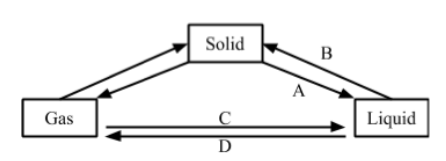
\includegraphics[width=0.6\textwidth]{./img/chem_I_matter_1.png}
	\end{center}
	
	\item Match each item in List A with the correct response in List B
	\begin{center}
		\begin{tabular}{|cp{8cm}|cp{3cm}|} \hline
			\multicolumn{2}{|c|}{List A} & \multicolumn{2}{|c|}{List B} \\ \hline
			I) & A process of separating a mixture of sodium chloride & A & Evaporation \\ 
			&  and ammonium chloride & B & Filtration \\
			II) & A method used to separate oil and water & C & Boiling \\
			III) & A method by which coloured substances are & D & Chrmoatography \\
			&  separated and identified & E & Distillation \\
			IV) & A method by which salt and water can be separated & F & Layer separation \\
			V) &  A method used to get the solvent from the solution & G & Decantation \\ 
			&  mixture & H & Sublimation \\ \hline
		\end{tabular}
	\end{center}
	
	\item Define matter
	
	\item Tell whether the following is a chemical change or physical change: Rotting of mango; Clouds changing into rain; Decaying of teeth
	
	\item State four difference between a chemical change and physical change
	
	\item The following figure shows the apparatus that can be used to separate three liquids: cooking oil, kerosene and water with density 0.92 g/cm$^3$, 0.65 g/cm$^3$, and 1.00 g/cm$^3$ respectively. \\
	\begin{center}
		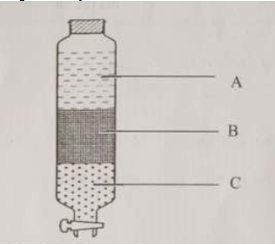
\includegraphics[width=0.5\textwidth]{./img/chem_I_matter_2.png}
	\end{center}
	Name the apparatus shown by the given figure. Giving a reason, identify liquids A and C. 
	
%%%%%%%%%%%%%%%%%%%%%%%%%%%%%%%%%%%%%%%%%%%%%%%%%%%%%%%%%%%%		
	\item Which method could be used to separate the products in the following equation? 
	\begin{center}
	Pb(NO$_3$)$_{2 (aq)}$ + 2KI$_{(aq)}$ $\rightarrow$ PbI$_{2 (S)}$ + 2KNO$_{3 (aq)}$ \\
	\textbf{colourless} \hspace*{2mm} \textbf{colourless} \hspace*{2mm} \textbf{yellow} \hspace*{2mm} \textbf{colourless}
	\end{center}
	\begin{enumerate}[topsep=0ex,itemsep=0ex,partopsep=1ex,parsep=1ex]
		\item[(A)] Chromatography
		\item[(B)] Crystallization
		\item[(C)] Distillation
		\item[(D)] Filtration
		\item[(E)] Condensation
	\end{enumerate}
	
	\item Briefly explain why the mixture with equal boiling point cannot be separated by simple fractional distillation
	
	\item Hygroscopic and deliquescent substances can be used as:
	\begin{enumerate}[topsep=0ex,itemsep=0ex,partopsep=1ex,parsep=1ex]
		\item[(A)] Oxidizing agents
		\item[(B)] Drying agents
		\item[(C)] Reducing agents
		\item[(D)] Weak electrolytes
		\item[(E)] Catalyst
	\end{enumerate}
	
	\item Water can be obtained from a solution of common salt by:
	\begin{enumerate}[topsep=0ex,itemsep=0ex,partopsep=1ex,parsep=1ex]
		\item[(A)] Evaporation
		\item[(B)] Simple distillation
		\item[(C)] Filtration
		\item[(D)] Condensation
		\item[(E)] Fractional distillation
	\end{enumerate}
	
	\item Suggest one best method for separating each of the following mixtures:
	\begin{enumerate}[topsep=0ex,itemsep=0ex,partopsep=1ex,parsep=1ex]
		\item[i)] Common salt and water
		\item[ii)] Iodine and sand
		\item[iii)] Pieces of iron and sand
	\end{enumerate}
\end{enumerate}


















\subsection{Air Combustion, Rusting and Fire Fighting}

\begin{enumerate}
	\item The substances that can be used to extinguish fire are:
	\begin{enumerate}[topsep=0ex,itemsep=0ex,partopsep=1ex,parsep=1ex]
		\item[(A)] Carbon dioxide and sand
		\item[(B)] Carbon dioxide and sugar
		\item[(C)] Nitrogen and sand
		\item[(D)] Nitrogen and water
	\end{enumerate}
	
	\item Flammable chemicals are those which:
		\begin{enumerate}[topsep=0ex,itemsep=0ex,partopsep=1ex,parsep=1ex]
		\item[(A)] Burn skin
		\item[(B)] Catch fire easily
		\item[(C)] Explode
		\item[(D)] Extinguish fire
	\end{enumerate}
	
	\item What do you understand by the following term: Flame
	
	\item The appropriate extinguisher used to put off fire caused by cooking oil is:
		\begin{enumerate}[topsep=0ex,itemsep=0ex,partopsep=1ex,parsep=1ex]
		\item[(A)] Water extinguisher
		\item[(B)] Carbon extinguisher
		\item[(C)] Wet chemical extinguisher
		\item[(D)] Dry air extinguisher
	\end{enumerate}
	
	\item Fill in the blanks: Three components of the fire triangle are heat, fuel and \rule{1.5cm}{0.15mm}.
	
	\item By using locally available materials in your school, state how the fire can be extinguished in the following situations: Kerosene spilled on the floor catches fire; Friend's clothes catch fire which gets out of her control
	
	\item Suggest the suitable method of preventing rust in the following: Moving parts of machines e.g. motorcycle chain; Motor vehicle (car) bodies
	
	\item Which gas is the least abundant gas in the air?
		\begin{enumerate}[topsep=0ex,itemsep=0ex,partopsep=1ex,parsep=1ex]
		\item[(A)] Nitrogen
		\item[(B)] Oxygen
		\item[(C)] Neon
		\item[(D)] Carbon dioxide
	\end{enumerate}
	
%%%%%%%%%%%%%%%%%%%%%%%%%%%%%%%%%%%%%%%%%%%%%%%%%%%%%%%%%%%%%%
	\item Which type of a fire is associated with electrical equipment?
	\begin{enumerate}[topsep=0ex,itemsep=0ex,partopsep=1ex,parsep=1ex]
		\item[(A)] Class E
		\item[(B)] Class C
		\item[(C)] Class F
		\item[(D)] Class B
		\item[(E)] Class A
	\end{enumerate}
	
	\item Which of the following is NOT among the composition of air?
	\begin{enumerate}[topsep=0ex,itemsep=0ex,partopsep=1ex,parsep=1ex]
		\item[(A)] Noble gases
		\item[(B)] Carbon dioxide
		\item[(C)] 
		\item[(D)] Hydrogen
		\item[(E)] Water vapor
	\end{enumerate}
	
	\item 
	\begin{enumerate}[topsep=0ex,itemsep=0ex,partopsep=1ex,parsep=1ex]
		\item[i)] State two conditions required for iron to rust
		\item[ii)] List two methods which are used to prevent rusting of iron
	\end{enumerate}
	
\end{enumerate}
























% Form II
\section{Form II Topics}
\subsection{Oxygen}

\begin{enumerate}
	\item Write a word equation for each of the following reaction: Calcium burns in oxygen
	
	\item Mention four chemical properties of Oxygen
	
	\item Write the names and formulae of the two chemicals that can be used in the preparation of oxygen gas
	
	\item State an appropriate method of collecting oxygen gas based on solubility and density of the gas in water
	
	\item How can oxygen gas be tested?
	
	\item List four uses of oxygen gas

%%%%%%%%%%%%%%%%%%%%%%%%%%%%%%%%%%%%%%%%%%%%%%%%%%%%%%%%
	\item Give the names or formula of the two chemicals that would be used in the laboratory to make each of the following gas. State a simple test that could be used to identify the gas. 
	\begin{enumerate}
		\item[i)] Oxygen
	\end{enumerate}
\end{enumerate}














\subsection{Hydrogen}

\begin{enumerate}
	\item Fill in the blank: A substance that speeds up a chemical reaction but remains chemically unchanged is called \rule{1.5cm}{0.15mm}.
	
	\item Hydrogen gas is prepared in the laboratory by reacting dilute hydrochloric acid and zinc granules
	\begin{enumerate}[topsep=0ex,itemsep=0ex,partopsep=1ex,parsep=1ex]
		\item[a.] Write an alternative acid that can be used to prepare hydrogen instead of dilute hydrochloric acid
		\item[b.] Give two physical and two chemical properties of hydrogen
	\end{enumerate}
	
	\item What will happen if a burning wooden splint is lowered in a test tube containing hydrogen gas?
	
	\item Give two uses of hydrogen gas in daily life
	
%%%%%%%%%%%%%%%%%%%%%%%%%%%%%%%%%%%%%%%%%%%%%%%%%%%%%	
	\item Give the names or formula of the two chemicals that would be used in the laboratory to make each of the following gas. State a simple test that could be used to identify the gas. 
	\begin{enumerate}
		\item[i)] Hydrogen
	\end{enumerate}

\end{enumerate}















\subsection{Water}

\begin{enumerate}
	\item When sugar is dissolved in water, a uniform mixture is formed. The resulting mixture is called a:
		\begin{enumerate}[topsep=0ex,itemsep=0ex,partopsep=1ex,parsep=1ex]
		\item[(A)] Solute
		\item[(B)] Solution
		\item[(C)] Solvent
		\item[(D)] Suspension
	\end{enumerate}

	\item Write a word equation for each of the following reactions: Sodium reacts with water
	
	\item What do you understand by the following terms: Water treatment; Water purification
	
	\item Mention six uses of water in economic activities
	
	\item How many atoms are their in a water molecule?

%%%%%%%%%%%%%%%%%%%%%%%%%%%%%%%%%%%%%%%%%%%%%%%%%%%%%%%
	\item State three main physical properties of water and show the usefulness of each property

\end{enumerate}
















\subsection{Fuels and Energy}

\begin{enumerate}
	\item Which of the following can be classified as a renewable source of energy? 
	\begin{enumerate}[topsep=0ex,itemsep=0ex,partopsep=1ex,parsep=1ex]
		\item[(A)] Biomass
		\item[(B)] Coal
		\item[(C)] Coke
		\item[(D)] Petroleum
	\end{enumerate}
		
	\item The process which produces energy in form of heat and light is called:
	\begin{enumerate}[topsep=0ex,itemsep=0ex,partopsep=1ex,parsep=1ex]
		\item[(A)] Decomposition
		\item[(B)] Combustion
		\item[(C)] Distillation
		\item[(D)] Sublimation
	\end{enumerate}
	
	\item Fill in the blank: A type of gas fuel derived from decomposing biological waste is called \rule{1.5cm}{0.15mm}.
	
%%%%%%%%%%%%%%%%%%%%%%%%%%%%%%%%%%%%%%%%%%%%%%%%%
	\item Give three examples in each of the following: 
	\begin{enumerate}
		\item[i)] Solid fuel
		\item[ii)] Gaseous fuel
	\end{enumerate}
	
\end{enumerate}















\subsection{Atomic Structure}

\begin{enumerate}
	\item Define the following term: Element
	
	\item The mass number of an atom is determined by:
	\begin{enumerate}[topsep=0ex,itemsep=0ex,partopsep=1ex,parsep=1ex]
		\item[(A)] Protons and neutrons
		\item[(B)] Protons and electrons
		\item[(C)] Neutrons and electrons
		\item[(D)] Protons alone
	\end{enumerate}
	
	\item Fill in the blank: The arrangement of electrons in different shells in the atom is called \rule{1.5cm}{0.15mm}.
	
%%%%%%%%%%%%%%%%%%%%%%%%%%%%%%%%%%%%%%%%%%%%%%%%%%%%%%%
	\item An atom M has an atomic number 14 and mass number 28.
	\begin{enumerate}
		\item[i)] What is the number of protons and neutrons?
		\item[ii)] Write the electronic configuration of atom M
	\end{enumerate}

	\item The mass number of a carbon atom that contains six protons, eight neutrons, and six electrons is:
	\begin{enumerate}[topsep=0ex,itemsep=0ex,partopsep=1ex,parsep=1ex]
		\item[(A)] 6
		\item[(B)] 14
		\item[(C)] 8
		\item[(D)] 12
		\item[(E)] 20
	\end{enumerate}
	
	\item Protons, neutrons and electrons particles are located in the atoms; fill in the missing information in below table about these particles. 
	\begin{center}
		\begin{tabular}{|c|c|c|c|} \hline
			\textbf{Particles} & \textbf{Relative Mass} & \textbf{Relative Charge} & \textbf{Location} \\ \hline
			Proton & & & \\ \hline
			Electron & $\frac{1}{1840}$ & & \\ \hline
			Neutron & & 0 & In the nucleus \\ \hline
		\end{tabular}
	\end{center}
	
\end{enumerate}









\subsection{Periodic Classification}

\begin{enumerate}
	\item An element X with atomic number 16 belongs to:
	\begin{enumerate}[topsep=0ex,itemsep=0ex,partopsep=1ex,parsep=1ex]
		\item[(A)] period 3, group III, valency of 2
		\item[(B)] period 3, group VI, valency of 2
		\item[(C)] period 3, group VI, valency of 6
		\item[(D)] period 6, group VI, valency of 6
	\end{enumerate}
	
	\item Which of the following electron configurations are of metals?
	\begin{enumerate}[topsep=0ex,itemsep=0ex,partopsep=1ex,parsep=1ex]
		\item[(A)] 2:8:1 and 2:5
		\item[(B)] 2:8:2 and 2:6
		\item[(C)] 2:8:3 and 2:8:8:1
		\item[(D)] 2:8:6 and 2:8:8:7
	\end{enumerate}
	
	\item Which of the following is a metal?
	\begin{enumerate}[topsep=0ex,itemsep=0ex,partopsep=1ex,parsep=1ex]
		\item[(A)] Water
		\item[(B)] Chlorine
		\item[(C)] Sodium
		\item[(D)] Nitrogen
	\end{enumerate}
	
	\item Which neutral atom has the same number of electrons as Mg$^{2+}$?
	\begin{enumerate}[topsep=0ex,itemsep=0ex,partopsep=1ex,parsep=1ex]
		\item[(A)] Magnesium
		\item[(B)] Sodium
		\item[(C)] Neon
		\item[(D)] Argon
	\end{enumerate}
	
%%%%%%%%%%%%%%%%%%%%%%%%%%%%%%%%%%%%%%%%%%%%%%%%%%
	\item Which of the following is the electronic configuration of an element Y found in period 3 and group II of the periodic table?
	\begin{enumerate}[topsep=0ex,itemsep=0ex,partopsep=1ex,parsep=1ex]
		\item[(A)] 2:8
		\item[(B)] 2:8:2
		\item[(C)] 2:6
		\item[(D)] 2:8:8:2
		\item[(E)] 2:8:4
	\end{enumerate}

	\item Use the knowledge of the periodic table to complete the table below. 
	\begin{center}
		\begin{tabular}{|cp{9.5cm}|cp{2cm}|} \hline
			\multicolumn{2}{|c|}{List A} & \multicolumn{2}{|c|}{List B} \\ \hline
			(i) & Its hydroxide is used in soil treatment & A & Barium \\ 
			(ii) & It is obtained from its ore in the blast furnace & B & Lithium \\ 
			(iii) & It gives a lilac colour when placed in a non-luminous flame & C & Iron \\
			(iv) & It forms an insoluble sulphate & D & Potassium \\
			(v) & It is in the same group in the periodic table with nitrogen & E & Oxygen \\
			(vi) & It reacts with hydrogen to form a compound which is a liquid & F & Fluorine \\
			& at room temperature & G & Sulphur \\
			(vii) & It is used in filament lamps & H & Argon \\
			(viii) & It is the strongest oxidizing agent among the halogens & I & Phosphorus \\
			(ix) & It exists in three main forms & J & Sodium \\
			(x) & Its chloride is added to food in order to give taste & K & Magnesium \\
			& & L & Carbon \\
			& & M & Neon \\
			& & N & Silicon \\
			& & O & Calcium \\ \hline
		\end{tabular}
	\end{center}
	
\end{enumerate}













\subsection{Formula Bonding and Nomenclature}

\begin{enumerate}
	\item The simplest formulas of a compound formed when combining 13g of aluminium and 17g of chlorine is
	\begin{enumerate}[topsep=0ex,itemsep=0ex,partopsep=1ex,parsep=1ex]
		\item[(A)] AlCl
		\item[(B)] Al$_2$Cl
		\item[(C)] Al$_3$Cl$_2$
		\item[(D)] AlCl$_3$
	\end{enumerate}
	
	\item A certain compound K contains 15.8\% carbon and 84.2\% sulphur. The molar mass of K is 76 g/mol. Determine its:
	\begin{enumerate}[topsep=0ex,itemsep=0ex,partopsep=1ex,parsep=1ex]
		\item[i)] simplest formula
		\item[ii)] molecular formula
	\end{enumerate}	
	
	\item Write the chemical formula for each of the following compounds:
	\begin{itemize}[topsep=0ex,itemsep=0ex,partopsep=1ex,parsep=1ex]
		\item[i)] Sodium carbonate
		\item[ii)] Calcium nitrate
		\item[iii)] Ammonium chloride
	\end{itemize}
	
	\item State the valency of the following atoms: Aluminium, Neon, Sulphur, Potassium
	
	\item Give the chemical formula for the combination of the following sets of ions: Mg$^{2+}$, PO$_4^{3+}$; Fe$^{3+}$, SO$_4^{2-}$
	
	\item Find the oxidation number of each of the underlined elements in the following: K\underline{Cl}O$_3$; \underline{Cr$_2$}O$_7^{2-}$
	
	\item Use the IUPAC system to name each of the following chemical compounds: CuO, CaSO$_4$, HNO$_3$, ZnCl$_2$
	
	\item Ability of an atom to gain or attract electrons towards itself \rule{1.5cm}{0.15mm}
	
	\item Write the names of the following radicals: SO$_3^{2-}$; ClO$_3^-$; PO$_4^{3-}$
	
	\item Calculate the oxidation state of the underlined element in the following compounds: NH$_4$\underline{Cl}; Al$_2$\underline{O$_3$}; Na$_2$\underline{S}O$_4$; \underline{Ca}(NO$_3$)$_2$

	\item The following table shows the name and the chemical formula of the product formed when ions combine together. Complete filling the table.
	\begin{center}
		\begin{tabular}{|p{3cm}|p{3cm}|p{3cm}|p{3cm}|} \hline
			Ion & Ion & Name & Formula \\ \hline
			Ca$^{2+}$ & Cl$^-$ & Calcium chloride & \\ \hline
			Al$^{3+}$ & SO$_4^{2-}$ & & Al$_2$(SO$_4$)$_3$ \\ \hline
			H$^+$ & & Hydrogen sulphate & \\ \hline
		\end{tabular}
	\end{center}
	
%%%%%%%%%%%%%%%%%%%%%%%%%%%%%%%%%%%%%%%%%%%%%%%%%%%%%%%%%%%%%	
	\item Chlorine ion, Cl$^-$ differs from chlorine atom because it has:
	\begin{enumerate}[topsep=0ex,itemsep=0ex,partopsep=1ex,parsep=1ex]
		\item[(A)] More protons
		\item[(B)] Less protons
		\item[(C)] More electrons
		\item[(D)] Less electrons
		\item[(E)] More neutrons
	\end{enumerate}
	
	\item 
	\begin{enumerate}[topsep=0ex,itemsep=0ex,partopsep=1ex,parsep=1ex]
		\item[i)] What type of a chemical bond is found between fluorine atoms in a fluorine molecule?
		\item[ii)] Name other type(s) of chemical bond formed by fluorine with other elements. Give an example of a compound in which fluorine form this type of bond.
	\end{enumerate}
	
\end{enumerate}















% Form III
\section{Form III Topics}
\subsection{Chemical Equations}

\begin{enumerate}
	\item Calculate the volume of water which was produced when 1,120 cm$^3$ of oxygen at s.t.p. was liberated during the decomposition of hydrogen peroxide. The density of water = 1.0 g/cm$^3$.

\end{enumerate}














\subsection{Hardness of Water}

\begin{enumerate}
	\item With the aid of a chemical equation, briefly explain how
	\begin{enumerate}[topsep=0ex,itemsep=0ex,partopsep=1ex,parsep=1ex]
		\item[i)] temporary hardness of water can be removed by boiling
		\item[ii)] permanent hardness of water can be removed by chemical means
	\end{enumerate}
	
	\item A student tested four samples of water, each 5 cm$^3$ from different areas of Kahama district by shaking with 3 drops of soap solution. The experiment was repeated by boiling each sample of water (5 cm$^3$) with 3 drops of soap solution. The observations were recorded in below table.
	\begin{center}
		\begin{tabular}{|c|c|c|} \hline
			\multirow{2}{*}{\textbf{Sample}} & \multirow{2}{*}{\textbf{Observation with Soap Solution}} & \textbf{Observation for Boiled Sample} \\ 
			& & \textbf{with Soap Solution} \\ \hline
			A & No lather & Lather \\ \hline
			B & Lather & Lather \\ \hline
			C & Lather & Lather \\ \hline
			D & No lather & No lather \\ \hline
		\end{tabular}
	\end{center}
	\begin{enumerate}[topsep=0ex,itemsep=0ex,partopsep=1ex,parsep=1ex]
		\item[i)] Which samples contain hard water?
		\item[ii)] Which sample contains temporary hard water? Give a reason. 
	\end{enumerate}
	
\end{enumerate}









\subsection{Acids, Bases and Salts}

\begin{enumerate}
	\item Using four examples, explain how the process of neutralization is important in day to day life. 
	
	\item A solution of pH 1.6 is best described as:
	\begin{enumerate}[topsep=0ex,itemsep=0ex,partopsep=1ex,parsep=1ex]
		\item[(A)] Weak acid
		\item[(B)] Strong base
		\item[(C)] Weak base
		\item[(D)] Strong acid
		\item[(E)] Neutral solution
	\end{enumerate}
	
	\item Give three applications of the process of neutralization in daily life.
	
\end{enumerate}









\subsection{The Mole Concept and Related Calculations}

\begin{enumerate}
	\item A student attempted to prepare hydrogen gas by reacting zinc metal with dilute sulphuric acid. In this experiment zinc metal granules of about 0.5 cm diameter and 0.20 moles of acid were used. The rate of formation of hydrogen gas was found to be slow. 
	\begin{enumerate}[topsep=0ex,itemsep=0ex,partopsep=1ex,parsep=1ex]
		\item[i)] Explain three ways in which the rate of formation of hydrogen gas could be increased.
		\item[ii)] If the student wanted 36 cm$^3$ of hydrogen gas at s.t.p., what amount of the acid would be required?
	\end{enumerate}
	
	\item How many moles of oxygen are required for the complete combustion of 2.2 g of C$_3$H$_8$ to form carbon dioxide and water?
		\begin{enumerate}[topsep=0ex,itemsep=0ex,partopsep=1ex,parsep=1ex]
		\item[(A)] 0.050 moles
		\item[(B)] 0.15 moles
		\item[(C)] 0.25 moles
		\item[(D)] 0.50 moles
		\item[(E)] 0.025 moles
	\end{enumerate}
	
	\item Compound X contains 24.24\% carbon, 4.04\% hydrogen and 71.72\% chlorine. Given that, the vapour density of X is 49.5.
		\begin{enumerate}[topsep=0ex,itemsep=0ex,partopsep=1ex,parsep=1ex]
		\item[i)] Calculate the molecular formula of the compound X
		\item[ii)] Draw and name the displayed\slash open structure formula of the possible isomer(s) from the molecular formula determined.
	\end{enumerate}
	
\end{enumerate}










\subsection{Volumetric Analysis}

\begin{enumerate}
	\item Suggest a suitable indicator for the following titrations:
		\begin{enumerate}[topsep=0ex,itemsep=0ex,partopsep=1ex,parsep=1ex]
		\item[i)] Hydrochloric acid against ammonia solution
		\item[ii)] Sulphuric acid against sodium hydroxide solution
		\item[iii)] Ethanoic acid against potassium hydroxide solution
	\end{enumerate}
\end{enumerate}








\subsection{Ionic Theory and Electrolysis}

\begin{enumerate}
	\item State three industrial applications of electrolysis
	
	\item How long a current of 5A should be passed through a solution of silver chloride in order to deposit 3.24 g of silver metal at the cathode? Given that, the electrochemical equivalent of silver = 1.118 $\times$ 10$^{-3}$ ge$^{-1}$. 
	
	\item A steady current of 2A was passed through a solution containing ions of a metal (X$^{2+}$) for nine minutes. The mass of metal X that was liberated were 0.3552 g. Calculate the molar mass of metal X. 
	
\end{enumerate}










\subsection{Chemical Kinetics, Equilibrium and Energetics}

\begin{enumerate}
	\item Hydrogen peroxide breaks down slowly to form water and oxygen; the reaction can be speed up by using a catalyst.
		\begin{enumerate}[topsep=0ex,itemsep=0ex,partopsep=1ex,parsep=1ex]
		\item[i)] How does the catalyst speed up the rate of reaction?
		\item[ii)] Name a possible catalyst that can be used to speed up the reaction.
		\item[iii)] Show that the catalyst always remains unchanged at the end of the reaction.
	\end{enumerate}
	
	\item Complete the following equations and determine the type of chemical reaction involved in each case.
		\begin{enumerate}[topsep=0ex,itemsep=0ex,partopsep=1ex,parsep=1ex]
		\item[i)] Zn$_{(S)}$ + H$_2$SO$_{4 (aq)} \rightarrow$
		\item[ii)] AgNO$_{3 (aq)}$ + NaCl$_{(aq)} \rightarrow$
		\item[iii)] N$_{2 (g)}$ + H$_{2 (g)} \rightarrow$
	\end{enumerate}
	
	\item In the graph below, curve 1 was obtained from the decomposition of 100 cm$^3$ of 1.0M hydrogen peroxide solution catalysed by manganese (IV) oxide, 2H$_2$O$_2 \rightarrow$ 2H$_2$O + O$_2$ \\
	\begin{center}
		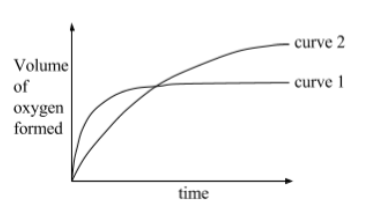
\includegraphics[width=0.5\textwidth]{./img/chem_III_kinetics_1.png}
	\end{center}
	Which alteration\slash change to the original experimental conditions would produce curve 2?
	\begin{enumerate}[topsep=0ex,itemsep=0ex,partopsep=1ex,parsep=1ex]
		\item[(A)] Lowering the temperature
		\item[(B)] Using less manganese (IV) oxide
		\item[(C)] Increasing the temperature
		\item[(D)] Adding some 0.1M H$_2$O$_2$ 
		\item[(E)] Using a different catalyst
	\end{enumerate}

	\item The reaction which produces methanol from carbon monoxide and hydrogen is represented by the equation CO$_{(g)}$ + 2H$_{2 (g)} \leftrightarrow$ CH$_3$OH$_{(g)}$ $\Delta$H = -94kJmol$^{-1}$. The reaction is carried out at high pressure to give a good yield of methanol
		\begin{enumerate}[topsep=0ex,itemsep=0ex,partopsep=1ex,parsep=1ex]
		\item[i)] Explain why increase in pressure gives a better yield of methanol
		\item[ii)] The value of $\Delta$H is negative. What does this tell about the reaction?
		\item[iii)] With a reason, state whether a high temperature or low temperature will give a better yield of methanol. 
	\end{enumerate}

\end{enumerate}










\subsection{Extraction of Metals}

\begin{enumerate}
	\item State four steps employed in the extraction of moderate reactive metals
	
	\item Copper can be obtained from the ore, copper pyrites (CuFeS$_2$). The ore is heated in a limited amount of air giving the following reaction:
	\begin{center}
		4CuFeS$_2$ + 11O$_2$ $\rightarrow$ 4Cu + 2Fe$_2$O$_3$ + 8SO$_2$
	\end{center}
	\begin{enumerate}[topsep=0ex,itemsep=0ex,partopsep=1ex,parsep=1ex]
		\item[i)] Calculate the maximum mass of copper that can be obtained from 367 kg of copper pyrites
		\item[ii)] State why the gaseous product from this reaction must not be allowed to escape into the atmosphere
	\end{enumerate}
	
	\item How long must a current of 4.00 A be applied to a solution of Cu$^{2+}$ (aq) to produce 2.0 grams of copper metal?
	\begin{enumerate}[topsep=0ex,itemsep=0ex,partopsep=1ex,parsep=1ex]
		\item[(A)] 2.4 $\times$ 10$^4$ s
		\item[(B)] 1.5 $\times$ 10$^3$ s
		\item[(C)] 7.6 $\times$ 10$^2$ s
		\item[(D)] 3.8 $\times$ 10$^2$ s
		\item[(E)] 12 $\times$ 10$^4$ s
	\end{enumerate}
	
	\item State three properties that make aluminium useful in overhead cables
	
	\item 
	\begin{enumerate}[topsep=0ex,itemsep=0ex,partopsep=1ex,parsep=1ex]
		\item[i)] Explain, in terms of electronic configurations, why sodium and potassium elements have similar chemical properties.
		\item[ii)] State the trend in reactivity of group I elements in the Periodic Table and give reasons for it.
	\end{enumerate}
	
	\item Describe the extraction of iron from the haematite ore and write all the chemical equations for the reactions involved in each stage of extraction.

\end{enumerate}









\subsection{Compounds of Metals}

\begin{enumerate}
	\item The metal nitrate which will NOT give a metal oxide on heating is:
	\begin{enumerate}[topsep=0ex,itemsep=0ex,partopsep=1ex,parsep=1ex]
		\item[(A)] Calcium nitrate
		\item[(B)] Silver nitrate
		\item[(C)] Lead nitrate
		\item[(D)] Copper nitrate
		\item[(E)] Zinc nitrate
	\end{enumerate}

	\item Find the oxidation state of sulphur in the sulphate ion, SO$_4^{2-}$
	
	\item List two classes of oxides. Give one example in each case.
	
	\item Briefly explain what will happen when
	\begin{enumerate}[topsep=0ex,itemsep=0ex,partopsep=1ex,parsep=1ex]
		\item[i)] iron (II) sulphate is exposed to air for a long time?
		\item[ii)] a bottle containing AgNO$_3$ is left open?
	\end{enumerate}
	
	\item Which of the following pairs of compounds can be used in the preparation of calcium sulphate?
	\begin{enumerate}[topsep=0ex,itemsep=0ex,partopsep=1ex,parsep=1ex]
		\item[(A)] Calcium carbonate and sodium sulphate
		\item[(B)] Calcium chloride and ammonium sulphate
		\item[(C)] Calcium hydroxide and barium sulphate
		\item[(D)] Calcium nitrate and lead (II) sulphate
		\item[(E)] Calcium chloride and barium sulphate
	\end{enumerate}

\end{enumerate}








% Form IV
\section{Form IV Topics}
\subsection{Nonmetals and their Compounds}

\begin{enumerate}
	\item Which of the following sets of elements is arranged in order of increasing electronegativity?
	\begin{enumerate}[topsep=0ex,itemsep=0ex,partopsep=1ex,parsep=1ex]
		\item[(A)] Chlorine, fluorine, nitrogen, oxygen, carbon
		\item[(B)] Fluorine, chlorine, oxygen, nitrogen, carbon
		\item[(C)] Carbon, nitrogen, oxygen, chlorine, fluorine
		\item[(D)] Nitrogen, oxygen, carbon, fluorine, chlorine
		\item[(E)] Fluorine, nitrogen, oxygen, chlorine, carbon
	\end{enumerate}
	
	\item Write balanced chemical equations to show how chlorine reacts with the following:
	\begin{enumerate}[topsep=0ex,itemsep=0ex,partopsep=1ex,parsep=1ex]
		\item[i)] water
		\item[ii)] aqueous iron (II) chloride solution
		\item[iii)] hydrogen sulphide
	\end{enumerate}
	
	\item Write the chemical formula of tetrachloromethane and state the type of bond that exists.
	
	\item The preparation of ammonia in the laboratory is done by heating any ammonium salt with an alkali.
	\begin{enumerate}[topsep=0ex,itemsep=0ex,partopsep=1ex,parsep=1ex]
		\item[i)] Write a balanced chemical equation for the preparation of ammonia gas.
		\item[ii)] State two uses of ammonia.
	\end{enumerate}
	
	\item Which among the following equations correctly shows the reaction between chlorine gas and water?
	\begin{enumerate}[topsep=0ex,itemsep=0ex,partopsep=1ex,parsep=1ex]
		\item[(A)] Cl$_{2 (g)}$ + H$_2$O$_{(l)}$ $\rightarrow$ Cl$_{2 (g)}$
		\item[(B)] 2Cl$_{2 (g)}^-$ + 2H$_2$O$_{(l)}$ $\rightarrow$ 4Cl$_{(aq)}$ + O$_{2 (g)}$ + 2H$_{2 (g)}$
		\item[(C)] Cl$_{2 (g)}$ + H$_2$O$_{(l)}$ $\rightarrow$ HCl$_{(aq)}$ + HOCl$_{(aq)}$
		\item[(D)] 2Cl$_{2 (g)}$ + 2H$_2$O$_{(l)}$ $\rightarrow$ 2HOCl$_{2 (aq)}$ + H$_{2 (aq)}$
		\item[(E)] 2Cl$_{2 (g)}$ + 3H$_2$O$_{(l)}$ $\rightarrow$ Cl$_{2 (g)}$ + 2H$_3$O$^+$
	\end{enumerate}
	
	\item Which among the following pair of substances are allotropes?
	\begin{enumerate}[topsep=0ex,itemsep=0ex,partopsep=1ex,parsep=1ex]
		\item[(A)] H$_2$O and H$_2$O$_2$
		\item[(B)] $^12$C and $^14$C
		\item[(C)] P$_4$ and P$_8$
		\item[(D)] H$_2$ and 2H$^+$
		\item[(E)] H$^+$ and H$_3$O
	\end{enumerate}
	
	\item Briefly explain what will happen when 
	\begin{enumerate}[topsep=0ex,itemsep=0ex,partopsep=1ex,parsep=1ex]
		\item[i)] concentrated sulphuric acid is exposed to the atomosphere.
	\end{enumerate}

\end{enumerate}








\subsection{Organic Chemistry}

\begin{enumerate}
	\item Which of the following compounds does NOT belong to the alkane homologous series?
	\begin{enumerate}[topsep=0ex,itemsep=0ex,partopsep=1ex,parsep=1ex]
		\item[(A)] C$_2$H$_4$
		\item[(B)] CH$_4$
		\item[(C)] C$_4$H$_{10}$
		\item[(D)] C$_3$H$_8$
		\item[(E)] C$_5$H$_{12}$
	\end{enumerate}
	
	\item You are provided with CH$_3$CH$_2$OH, CH$_3$CH$_2$CH$_3$, CH$_3$COOH, and CH$_2$=CH$_2$. 
	\begin{enumerate}[topsep=0ex,itemsep=0ex,partopsep=1ex,parsep=1ex]
		\item[i)] Which compounds are gases at room temperature? 
		\item[ii)] How can you distinguish compound CH$_3$CH$_2$CH$_3$ and CH$_2$=CH$_2$?
		\item[iii)] Which compound would react with sodium carbonate? Write the balanced chemical equation for the reaction. 
	\end{enumerate}
	
	\item Which of the following hydrocarbons does NOT belong to the same homologous series as the others?
	\begin{enumerate}[topsep=0ex,itemsep=0ex,partopsep=1ex,parsep=1ex]
		\item[(A)] CH$_4$
		\item[(B)] C$_3$H$_8$
		\item[(C)] C$_4$H$_{10}$
		\item[(D)] C$_6$H$_{12}$
		\item[(E)] C$_2$H$_{12}$
	\end{enumerate}
	
	\item Give the names or formula of the two chemicals that would be used in the laboratory to make each of the following gas. State a simple test that could be used to identify the gas. 
	\begin{enumerate}[topsep=0ex,itemsep=0ex,partopsep=1ex,parsep=1ex]
		\item[i)] Carbon dioxide
	\end{enumerate}
	
	\item Name the following compounds according to the IUPAC system
	\begin{enumerate}[topsep=0ex,itemsep=0ex,partopsep=1ex,parsep=1ex]
		\item[i)] 
		\item[ii)]
		\item[iii)] 
	\end{enumerate}
	
\end{enumerate}











\subsection{Soil Chemistry}

\begin{enumerate}
	\item Define the following terms:
	\begin{enumerate}[topsep=0ex,itemsep=0ex,partopsep=1ex,parsep=1ex]
		\item[i)] Soil
		\item[ii)] Leaching
		\item[iii)] Denitrification
	\end{enumerate}
	
	\item The table indicates the pH values of soil for some crops to grow
	\begin{center}
		\begin{tabular}{|c|c|} \hline
			\textbf{Crops} & \textbf{Soil pH} \\ \hline
			Tomato & 7.0 \\ \hline
			Bean & 6.0 \\ \hline
			Cabbage & 5.4 \\ \hline
			Cauliflower & 5.6 \\ \hline
			Celery & 6.3 \\ \hline
			Lettuce & 6.1 \\ \hline
			Onions & 5.7 \\ \hline
			Swede & 5.3 \\ \hline
			Parsley & 5.1 \\ \hline
		\end{tabular}
	\end{center}
	Which crop grows best in the:
	\begin{enumerate}[topsep=0ex,itemsep=0ex,partopsep=1ex,parsep=1ex]
		\item[i)] Most acidic soil?
		\item[ii)] Least acidic soil?
		\item[iii)] Neutral soil?
	\end{enumerate}
	
	\item Addition of inorganic fertilizers in the farm is not as important as addition of organic manure. Discuss the correctness of this statement in four points. 
	
\end{enumerate}










\subsection{Pollution}

\begin{enumerate}
	\item Explain five methods to prevent terrestrial pollution. 
	
\end{enumerate}




%\subsection{Qualitative Analysis}
\subsection{Multiple Topics}

\begin{enumerate}
	\item Match the items in List A with the responses in List B
	\begin{center}
		\begin{tabular}{|cp{9.5cm}|cp{2cm}|} \hline
			\multicolumn{2}{|c|}{List A} & \multicolumn{2}{|c|}{List B} \\ \hline
			(i) & An element with electronic configuration of 2:8 & A & Flourine \\
			(ii) & An element in which its oxide can be prepared by the action & B & Rhombic \\
			& of nitric acid and heat & C & Amorphous \\
			(iii) & An element which acts as an oxidant or reductant & D & Diamond \\
			(iv) & A gas that explodes when a flame is applied in the presence of & E & Argon \\
			& air & F & Zinc \\
			(v) & A gas which is prepared in the laboratory by isolation from air & G & Phosphorus \\
			(vi) & An element with atomic mass of 40 & H & Nitrogen \\
			(vii) & An element which reacts with water to produce hydroxide and & I & Hydrogen \\
			& hydrogen gas & J & Mercury \\
			(viii) & An element which is used in making jewellers & K & Neon \\
			(ix) & An element which is an allotrope of sulphur & L & Sulphur \\
			(x) & The most electronegative element & M & Oxygen \\
			& & N & Potassium \\
			& & O & Chlorine \\ \hline 
		\end{tabular}
	\end{center}
	
	\item Match the items in List A with the responses in List B
	\begin{center}
		\begin{tabular}{|cp{9.5cm}|cp{2cm}|} \hline
			\multicolumn{2}{|c|}{List A} & \multicolumn{2}{|c|}{List B} \\ \hline
			(i) & Its hydroxide is used in soil treatment & A & Barium \\
			(ii) & It is obtained from its ore in the blast furnace & B & Lithium \\
			(iii) & It gives a lilac colour when placed in a non-luminous flame & C & Iron \\
			(iv) & It forms an insoluble sulphate & D & Potassium\\
			(v) & It is in the same group in the periodic table with nitrogen & E & Oxygen\\
			(vi) & It reacts with hydrogen to form a compound which is a liquid & F & Fluorine \\
			& at room temperature & G & Sulphur \\
			(vii) & It is used in filament lamps & H & Argon \\
			(viii) & It is the strongest oxidizing agent among the halogens & I & Phosphorus \\
			(ix) & It exists in three main forms & J & Sodium \\
			(x) & Its chloride is added to food in order to give taste & K & Magnesium \\
			& & L & Carbon \\
			& & M & Neon \\
			& & N & Silicon \\
			& & O & Calcium \\ \hline
		\end{tabular}
	\end{center}

\end{enumerate}










% Form V and VI
%\section{Advance Level Topics}
%\subsection{The Atom}
%\subsection{Chemical Bonding}
%\subsection{Gases}
%\subsection{Relative Molecular Masses in Solution}
%\subsection{Two Component Liquids Systems}
%\subsection{Energetics}
%\subsection{Selected Compounds of Metals}
%\subsection{Transition Elements}
%\subsection{Aliphatic Hydrocarbons}
%\subsection{Aromatic Hydrocarbons}
%\subsection{Halogen Derivatives of Hydrocarbons}
%\subsection{Hydroxyl Compounds}
%\subsection{Carbonyl Compounds}

%\subsection{Chemical Equilibrium}
%\subsection{Chemical Kinetics}
%\subsection{Electrochemistry}
%\subsection{Acids, Bases and Salts}
%\subsection{Solubility, Solubility Product and Ionic Product}
%\subsection{Extraction of Metals}
%\subsection{Amines}
%\subsection{Polymers}
%\subsection{Environmental Chemistry}
%\subsection{Soil Chemistry}
%\subsection{Chemical Analysis}

\section{Form VI NECTA Chemistry Exam - 2017}

%%%%%%%% Mathematics %%%%%%%%
\chapter{Mathematics}
% Format
\section{NECTA Mathematics Exam Format}
\label{sec:math-format}

%%%%%%%%%%%%%%%%%%%%%%%%%%%%%
%-----------------------------Form II------------------------------------
%%%%%%%%%%%%%%%%%%%%%%%%%%%%%
\subsection{Form II}
\noindent The following format for the Form Two National Assessment (FTNA) is based on the revised version of the Basic Mathematics Syllabus for Ordinary Secondary Education of 2005. The exam is intended to assess the competences acquired by the students after two years of study. The following information was taken from The National Examinations Council of Tanzania - Form Two National Assessment Formats %CITE!!!!!!!!!!!!!!!!!!

\subsubsection{General Objectives}
\noindent The general objectives of the Basic Mathematics assessment are to test students' ability to:
\begin{enumerate}[topsep=1ex,itemsep=0ex,partopsep=1ex,parsep=1ex]
	\item Perform computations on numbers, algebraic terms and radicals
	\item Use approximations in solving simple problems
	\item Convert and do computations on basic units, decimals, percentages and fractions
	\item Construct and draw geometrical figures as well as finding angles, perimeters and areas of simple geometrical figures
	\item Compute ratios, profit and loss
	\item Draw graphs of linear equations, solve linear equations in one or two unknowns, solve linear inequalities in one unknown, solve quadratic equations and transpose formulae
	\item Derive and apply the laws of exponents and logarithms
	\item Do calculations using mathematical tables
	\item Prove and apply congruence and similarity of figures
	\item Represent reflections, rotations, translations and enlargement geometrically
	\item Determine sine, cosine and tangent of angles and hence apply them in solving problems
	\item Represent and interpret statistical data collected from real life situations
	\item Perform operations on sets and apply sets to solve problems
\end{enumerate}

\subsubsection{General Competences}
\noindent The FTNA will specifically test the students' ability to:
\begin{enumerate}[topsep=1ex,itemsep=0ex,partopsep=1ex,parsep=1ex]
	\item Distinguish different types of numbers
	\item Estimate and compute numbers accurately
	\item Convert units, decimals, percentages and fractions
	\item Handle mathematical instruments in constructing and drawing geometrical figures
	\item Solve problems on geometry, ratio, profit and loss
	\item Draw graph and interpret linear equations
	\item Find perimeters and areas of simple geometrical figures
	\item Find relationships among logarithms, exponents, radicals, right angled triangles and trigonometric ratios
	\item Use mathematical tables in computations
	\item Verify laws and prove theorems
	\item Do scale drawing and geometrical transformations
	\item Solve problems on quadratic equations
	\item Organize and interpret data
	\item Apply set operations in solving problems
\end{enumerate}

\subsubsection{Assessment Rubric}
\noindent The assessment consists of \textbf{one (1)} theory paper. The duration of the exam is \textbf{2 hours and 30 minutes}. The paper consists of \textbf{ten (10)} short-response questions (10 marks each). The students are required to attempt \textbf{all} questions, showing all work clearly.  

\subsubsection{Assessment Topics}
\begin{center}
\begin{tabular}{cl|c|c|c|} \\ \hline
\multicolumn{1}{|c|}{\textbf{S\slash n}} & \multicolumn{1}{c|}{\textbf{Topic(s)}} & \textbf{Form(s)} & \textbf{Pts} & \textbf{Total} \\ \hline \hline
\multicolumn{1}{|c|}{1} &  & I & 10 & \multirow{10}{*}{100} \\ \cline{1-4}
\multicolumn{1}{|c|}{2} &  & II & 10 & \\ \cline{1-4}
\multicolumn{1}{|c|}{3} &  & II & 10 & \\ \cline{1-4}
\multicolumn{1}{|c|}{4} &  & IV & 10 & \\ \cline{1-4}
\multicolumn{1}{|c|}{5} &  & I\slash II & 10 & \\ \cline{1-4}
\multicolumn{1}{|c|}{6} &  & I\slash III & 10 & \\ \cline{1-4}
\multicolumn{1}{|c|}{7} &  & I & 10 & \\ \cline{1-4}
\multicolumn{1}{|c|}{8} &  & III & 10 & \\ \cline{1-4}
\multicolumn{1}{|c|}{9} &  & II\slash IV & 10 & \\ \cline{1-4}
\multicolumn{1}{|c|}{10} &  & II & 10 & \\ \hline
\end{tabular}
\end{center}

%\subsubsection{Assessment Topics}
%\noindent The following table shows the topics assessed in the FTNA as well as the percentage they have appeared in past examinations. 
%\begin{center}
%	\begin{tabular}{|c|l|c|} \hline
%		Form & \multicolumn{1}{|c|}{Topic} & Percentage [\%] \\ \hline
%		\multirow{11}{*}{I} 	& Numbers				& \\ \cline{2-3}
%						& Fractions				& \\ \cline{2-3}
%						& Decimals and Percentages	& \\ \cline{2-3}
%						& Units					& \\ \cline{2-3}
%						& Approximations		 	& \\ \cline{2-3}
%						& Geometry 				& \\ \cline{2-3}
%						& Algebra					& \\ \cline{2-3}
%						& Ratio, Profit and Loss		& \\ \cline{2-3}
%						& Coordinate Geometry		& \\ \cline{2-3}
%						& Perimeters and Areas		& \\ \cline{2-3}
%						& Exponents and Radicals	& \\ \hline
%		\multirow{9}{*}{II} 	& Quadratic Equations		& \\ \cline{2-3}
%						& Logarithms				& \\ \cline{2-3}
%						& Congruence				& \\ \cline{2-3}
%						& Similarity				& \\ \cline{2-3}
%						& Geometrical Transformations	& \\ \cline{2-3}
%						& Pythagoras Theorem		& \\ \cline{2-3}
%						& Trigonometry				& \\ \cline{2-3}
%						& Sets					& \\ \cline{2-3}
%						& Statistics				& \\ \hline
%	\end{tabular}
%\end{center}

%%%%%%%%%%%%%%%%%%%%%%%%%%%%%
%-----------------------------Form IV------------------------------------
%%%%%%%%%%%%%%%%%%%%%%%%%%%%%
\subsection{Form IV}
\noindent The following format for the Form Four Certificate of Secondary Education (CSEE) is based on the revised version of the Basic Mathematics Syllabus for Ordinary Secondary Education of 2005. The exam is intended to assess the competences acquired by the students after four years of study. The following information was taken from The National Examinations Council of Tanzania - Certificate of Secondary Education Examination Formats %CITE!!!!!!!!!!!!!!!!!!

\subsubsection{General Objectives}
\noindent The general objectives of the Basic Mathematics assessment are to test students' ability to:
\begin{enumerate}[topsep=1ex,itemsep=0ex,partopsep=1ex,parsep=1ex]
	\item Mathematical competences among candidates in solving practical problems in daily life have been developed
	\item Mathematical concepts can be applied by candidates in interpreting situations at local and global levels
	\item Candidates are able to use mathematical knowledge, techniques and life skills for studying mathematics and related subjects
	\item Candidates have been adequately prepared for higher studies
\end{enumerate}

\subsubsection{General Competences}
\noindent The FTNA will specifically test the students' ability to:
\begin{enumerate}[topsep=1ex,itemsep=0ex,partopsep=1ex,parsep=1ex]
	\item Think critically and logically in interpreting and solving problems
	\item Use mathematical language in explaining and clarifying mathematical ideas
	\item Apply mathematical knowledge and techniques in other fields
\end{enumerate}

\subsubsection{Examination Rubric}
\noindent The examination consists of \textbf{one (1)} theory paper. The duration of the exam is \textbf{3 hours}. The paper consists of \textbf{sixteen (16)} short answer questions categorized into section A and B. Section A consists of \textbf{ten (10)}questions (6 marks each). Section B has \textbf{six (6)} questions (10 marks each). The students are required to attempt \textbf{all} questions in section A and \textbf{four (4)} in section B, clearly showing all workings. \\

\noindent Unlike other subjects present in this manual, the Basic Mathematics examination follows a special format. The format requires specific questions to cover specific topics (see table below). For example, Question 2 will \emph{always} be about exponents, radicals, and/or logarithms. Similarly, Question 11 will \emph{always} cover the topic of linear programming. Thus, it is possible for a student to effectively pass their exam, even by knowing just \emph{two} topics very well (e.g Statistics and Accounts). Of course, it is not necessarily recommended to have students only focus on learning a few select topics, as this does not encourage thorough learning of the material, but it can be used as a motivator to students who have already written themselves off for the Math NECTA.

\begin{center}
\begin{tabular}{cl|c|c|c|} \\ \hline
\multicolumn{1}{|c|}{\textbf{S\slash n}} & \multicolumn{1}{c|}{\textbf{Topic(s)}} & \textbf{Form(s)} & \textbf{Pts} & \textbf{Total} \\ \hline \hline
\multicolumn{5}{|c|}{\textbf{SECTION A (60 MARKS)}} \\ \hline
\multicolumn{1}{|c|}{1} & Numbers\slash Fractions\slash Decimals and Percentages\slash Approximations & I & 6 & \multirow{10}{*}{60} \\ \cline{1-4}
\multicolumn{1}{|c|}{2} & Exponents\slash Radicals\slash Logarithms & II & 6 & \\ \cline{1-4}
\multicolumn{1}{|c|}{3} & Algebra\slash Sets & II & 6 & \\ \cline{1-4}
\multicolumn{1}{|c|}{4} & Coordinate Geometry\slash Vectors & IV & 6 & \\ \cline{1-4}
\multicolumn{1}{|c|}{5} & Geometry\slash Perimeter and Area\slash Congruence\slash Similarity & I\slash II & 6 & \\ \cline{1-4}
\multicolumn{1}{|c|}{6} & Units\slash Rates and Variations & I\slash III & 6 & \\ \cline{1-4}
\multicolumn{1}{|c|}{7} & Ratio, Profit and Loss & I & 6 & \\ \cline{1-4}
\multicolumn{1}{|c|}{8} & Sequences and Series & III & 6 & \\ \cline{1-4}
\multicolumn{1}{|c|}{9} & Trigonometry\slash Pythagoras Theorem & II\slash IV & 6 & \\ \cline{1-4}
\multicolumn{1}{|c|}{10} & Quadratic Equations & II & 6 & \\ \hline
\multicolumn{5}{|c|}{\textbf{SECTION B (40 MARKS - CHOOSE 4)}} \\ \hline
\multicolumn{1}{|c|}{11} & Linear Programming & IV & 10 & \multirow{6}{*}{40} \\ \cline{1-4}
\multicolumn{1}{|c|}{12} & Statistics & III & 10 & \\ \cline{1-4}
\multicolumn{1}{|c|}{13} & Three Dimensional Figures\slash Circles\slash Earth as a Sphere & III\slash IV & 10 & \\ \cline{1-4}
\multicolumn{1}{|c|}{14} & Accounts & III & 10 & \\ \cline{1-4}
\multicolumn{1}{|c|}{15} & Matrices and Transformations & IV & 10 & \\ \cline{1-4}
\multicolumn{1}{|c|}{16} & Probability\slash Functions\slash Relations & III\slash IV & 10 & \\ \hline

\end{tabular}
\end{center}

%Letter grades are assigned based on the following scale for Form IV NECTA exams:
%\begin{center}
%\begin{tabular}{c|c}
%Score & Grade \\ \hline
%81 - 100 & A \\
%61 - 80 & B \\
%41 - 60 & C \\
%21 - 40 & D \\
%0 - 20 & F \\
%\end{tabular}
%\end{center}
%
%Have students plan ahead of time to formulate a strategy for the exam. Which 4 topics does each student feel most comfortable with from Section B? Students should have 1 fall-back topic in case one of their preferred topics is particularly challenging on an exam. Advise students to begin with problems from Section B, as these carry more marks and therefore should have more time dedicated to them. Which topics from Section A are strengths for a student, and which ones are weaknesses? Students should answer their strong topics first, and use whatever time they have remaining for weaker topics.
%
%Planning ahead and utilizing a strategy for taking the NECTA exam will give students added confidence in their test-taking abilities and will also give them a strategy for what topics to study in most detail leading up to the exam. Make sure to give students plenty of practice exams before the actual NECTA! Many students only have one opportunity to familiarize themselves with the layout of the test during Mock Examinations a few months ahead of time, but this is not enough. Comfort and confidence in one's math abilities come from practice, practice and more practice!



% Form I
\section{Form I Topics}
\subsection{Numbers, Fractions, Decimals, Approximations}
	
\begin{enumerate}


			\subsubsection{Evaluation / BODMAS}
%evaluate (BODMAS)
	\item Evaluate $[9876 - 4321] \div 55 - 7 \times 6 + 3$
	
	\item Evaluate $24 \times (10 + 54) \div 8 - 2$
	
	\item Using mathematical tables, evaluate $\cfrac{(36.12)^3 \times 750.9}{(113.2)^2 \times \sqrt{92.5}}$
	
%fraction form	 	
	 \item Evaluate $\cfrac{ \frac{1}{25} + 0.28 + 1\frac{17}{25} }{ 3\frac{1}{5} \div \frac{0.32}{0.15} }$ Give your answer in fraction form.
	 
	 \item Evaluate $\cfrac{0.0084 \times 1.23 \times 3.5}{2.87 \times 0.056}$ with using mathematical tables and express the answer as a fraction in its simplest form.

%numbers - standard form
	\item Given $x = 4.5 \times 10^{-7}$ and $z = 7.2 \times 10^5$, find $y$ in standard form if $z = xy$.
	
	\item Given $x = 1.6 \times 10^8$ and $y = 5.6 \times 10^4$, find $z$ in standard form if $ xz = y$.
	
	\item Compute $0.678 \times 145$ and express the answer in standard form.
	
	\item Given that $M = 4 \times 10^3$, express $\frac{1}{M}$ in standard form.


			\subsubsection{GCF, LCM}
%GCF, LCM	
	\item Find the product of the LCM and GCF of 40, 120 and 240.
	
	\item Find (a) GCF and (b) LCM of 15, 35 and 56.
	
	\item Two numbers, 60 and $n$, have the lowest common multiple (LCM) of 420. If $n$ is a multiple of 6 less than 90, find:
		\begin{itemize}
		\item[(i)] the possible values of $n$.
		\item[(ii)] the greatest common factor (GCF) of the two numbers.
		\end{itemize}	
		
	\item The GCF and LCM of $y$, 18 and 60 are 6 and 360 respectively. Find the value of $y$.
		
	\item The numbers 28, 41, 42, 59, 70 belong to the set of natural numbers. By using these numbers:
		\begin{itemize}
		\item[(i)] calculate the difference between the least common multiple (LCM) of the prime numbers and the greatest common factor (GCF) of the remaining numbers.
		\item[(ii)] express the answer obtained in (i) above in the standard form $A \times 10^n$ correct to two significant figures where $1 \leq A < 10$ and $n$ is an integer.
		\end{itemize}			 
	
	
			\subsubsection{Integers}
%integers
	\item By using properties of integers, give reasons why each of the following expressions are equal:
		\begin{itemize}
		\item[(i)] $(15 \times 17) \times 12 = 17 \times (15 \times 12)$
		\item[(ii)] $15 \times (17 + 12) = (15 \times 17) + (15 \times 12)$
		\end{itemize}
		
	\item An aeroplane traveling at an altitude of 3200 metres makes a climb of 1500 metres, followed by a drop of 100 metres.
		\begin{itemize}
		\item[(a)] Represent the plane's altitude as a sum of positive and negative integers.
		\item[(b)] What is the planes altitude after the drop?
		\end{itemize}
	

		\subsubsection{Recurring Decimals}	 
%recurring decimals
	 
	 \item Express $1.8\dot{6}$ as an improper fraction in its simplest form.
	 
	 \item Change $0.\dot{1}2\dot{3}$ into a fraction.
	 
	 \item Express $23.\dot{1}2\dot{3}$ as a fraction.
	 
	 \item Express $2.\dot{1}35\dot{3}$ as a fraction.
	 
	 \item Express $2.\dot{1}4\dot{6}$ as a fraction.
	 
	 \item Change $0.0\dot{1}$ into a fraction.
	 
	 \item Determine the fractional notation for $0.6\dot{3}$.
	 
	 \item Express $1.\dot{2}1\dot{3}$ as a rational number.
	
	\item Express the following recurring decimal number as a rational number: $0.\dot{6}5\dot{7}$.
	 
	 \item Express $0.8\dot{3}$ in the form $\frac{a}{b}$ where $a$ and $b$ are integers such that $b \neq 0$.
	 
	 \item Express $0.\dot{3}0\dot{3}$ as a fraction, i.e. $\frac{a}{b}$ where $a$ and $b$ are integers and $b \neq 0$.

			\subsubsection{Word Problems}
	\item Mr. Bean lived a quarter of his life as a child, a fifth as a teenager and a third as an adult. He then spent 13 years in his old age. How old was he when he died?	
			
	\item Mary received a certain amount of money from her father to go to school. She spent one third in her journey to school. At school she paid two thirds of the remaining amount as school fees and remained with 24,000 /= as her pocket money. Showing the procedure, calculate the total amount of money she received from her father. 
			
	\item A certain worker used his salary as follows: 20\% on house rent, 45\% on food, 10\% on refreshment and 15\% on school fees. If he\slash she was left with Tsh. 22,000, determine:
		\begin{itemize}
		\item[(i)] the salary of the worker.
		\item[(ii)] the amount of money which he\slash she spent on food.
		\end{itemize}

		\subsubsection{Approximations}	
%approximations - give to _ decimal places
	\item By using mathematical tables, evaluate $\cfrac{\sqrt[3]{0.0072} \times (81.3)^2}{\sqrt{23140}}$ to three significant figures.
	
	\item By using mathematical tables, evaluate $\cfrac{(28.32)^4 \times 0.03574}{87.57}$. Give your final answer in standard form, to three significant figures.
	
	\item If $a = 2.432 \times 10^4$, $b = 7.42 \times 10^{-2}$ and $c = 0.0324 \times 10^{-2}$, find the value of $R$ in standard form correct to two decimal places given that $R = \cfrac{ab}{c}$.
	
	\item Using mathematical tables, evaluate the expression: $\cfrac{(28.32)^2 \times 0.3574}{\sqrt{8.732}}$. Give the answer correct to four decimal places.
	 
	 \item By using mathematical tables evaluate the expression $\cfrac{237.8 \times 0.0873}{67890}$. Give the answer to four figures.
	 
	 \item Given that $\sqrt{3} = 1.7321$, calculate the value of $\cfrac{2}{\sqrt{3} - 1}$ correct to 4 decimal places.

%round off, estimate
	\item Estimate he value of $\cfrac{57.2 \times 110}{2.146 \times 46.9}$ correct to one (1) significant figure.
	 
	 \item 
	 	\begin{itemize}
	 	\item[(a)] Find the value of the expression $\left(\cfrac{4.75 + 1.31}{3.13}\right)^2$ giving your answer in three decimal places.
	 	\item[(b)] By rounding each term of the expression in (a) above to one significant figure, obtain a rough estimate of the expression.
	 	\end{itemize}
	 
	 \item 
	 	\begin{itemize}
	 	\item[(a)] Round off each of the following numbers to one decimal place. $L = 20.354$, $M = 40.842$, $N = 10.789$
	 	\item[(b)] Use the result obtained in (a) above to find the value of $x$ given that $x = \cfrac{LM}{N}$.
	 	\end{itemize}
	 	
	\item Round each of the numbers $x = 2.354$, $y = 4.843$ and $z = 1.789$ to one decimal place and then use the results obtained to find the value of $A$ to two significant figures given that $A = \cfrac{xy}{z}$.
	 
	\item Express 0.05473
		\begin{itemize}
		\item[(i)] correct to three (3) significant figures
		\item[(ii)] correct to three (3) decimal places
		\item[(iii)] in standard form
		\end{itemize}
	
	\item Write 624.3278 correct to
		\begin{itemize}
		\item[(i)] five significant figures
		\item[(ii)] three decimal places
		\end{itemize}



\end{enumerate}	

\subsection{Algebra}
\subsection{Approximations}
\subsection{Geometry}
	
\begin{enumerate}
		\item 
		\begin{itemize}
		\item[(i)] What is the sum of the interior angles of an octagon?
		\item[(ii)] Find the size of the exterior angle of a regular octagon.
		\end{itemize}
		
	\item Calculate the size of an interior angle of a regular nonagon.
	
	\item A regular polygon has an exterior angle of $36^\circ$. Calculate:
		\begin{itemize}
		\item[(a)] the size of an interior angle
		\item[(b)] the number of sides of the polygon
		\end{itemize}
	
	\item An exterior angle of a regular polygon has degree measure of 22$^1/_2$. Find the sum of degree measure of all the interior angles.
	
	\item The interior angle of a regular polygon is $120^\circ$ greater than the exterior angle. Find the number of sides of the polygon.
	
	\item If the interior angle of a regular polygon is $6^1/_2$ times the exterior angle, how many sides does the polygon have?


\end{enumerate}

\subsection{Algebra}
\subsection{Numbers (II)}
\subsection{Ratio, Profit and Loss}
\begin{enumerate}

		\subsubsection{Ratio}
	\item An alloy consists of three metals A, B and C in the proportions $A:B = 3:5$ and $B:C = 7:6$. Calculate the proportion $A:C$.		
		
	\item Given the ratios:\\
	$A : B = 2 : 3$\\
	$B : C = 6 : 7$\\
	Calculate the ratio of $A : C$.
	
	\item Express $2\frac{1}{2} : 3$ as integers in a simplified form.
	
	\item If it is known that $x:y = 5:1$ find the value of $\cfrac{x + y}{3x - 4y}$.
	
	\item Three numbers $d$, $m$ and $n$ are in the ratio of $3:6:4$ respectively. Find the value of $\cfrac{4d - m}{m + 2n}$.
	
	\item A, B and C are to share Tshs. 120,000/= in the ratio $2:3:5$ respectively. How much will each get?
	
	\item Three people share a property in the ratio $2:x:y$. It is known that $y = x + 2$. If the largest shareholder had Tsh. 39,100/= in monetary terms, find the value of this property.
	
	\item The ratio of men : women : children living in Mkuza village is 6 : 7 : 3. If there are 42,000 women, find how many:
		\begin{itemize}
		\item[(a)]
			\begin{itemize}
			\item[(i)] children live in Mkuza village.
			\item[(ii)] people altogether live in Mkuza village.
			\end{itemize}
		\item[(b)] The 42,000 women is an increase of 20\% on the number of women ten years ago. How many women lived in the village?
		\end{itemize}
		
	\item An amount of Tshs. 12,000 is to be shared among Ali, Anna and Juma in the ratio 2 : 3 : 5 respectively. How much will each get?

	\item The are of two circles are in the ratio of 16 : 9. Calculate the radius of the smaller circle when the radius of the larger one is 24 cm.
	
	\item The ratio of the areas of two circles is 50 : 72. If the radius of the smaller circle is 15 cm, find the radius of the larger circle.
	
	\item The sides of a rectangle are in the ratio 3 : 5. If the perimeter of this rectangle is 800 cm, find the dimensions of the rectangle.
	
	\item The distance between two towns on a map of scale 1 : 5,000,000 is 9 cm. Find the actual distance between the towns in kilometres.
	
	\item A building 250 metres high is represented by a line segment of length 5 cm. Find the scale of drawing.
	
	\item An area of 24.7 cm$^2$ was plotted on a map of a scale 1 : 50,000. What was this area, in square kilometres, on the Earth's surface?
	
	
		\subsubsection{Profit and Loss}
%profit and loss
	\item 
		\begin{itemize}
		\item[(a)] John and Paul started a tailoring business and invested shs 110,250/= and 220,500/= respectively. If the profit after the first six months was shs 50,970/=, how much did Paul get if they agreed to share it according to the amount they invested.
		\item[(b)] Mary paid shs 800,000/= for a computer and sold it the following year for shs 600,000/=. Find the percentage loss she got.
		\end{itemize}
		
	\item By selling an article at shs. 22,500/= a shopkeeper makes a loss of 10\%. At what price must the shopkeeper sell the article in order to get a profit of 10\%?
	
	\item Neema bought a tray of eggs (containing 30 eggs) for shs. 2,000/=. She boiled the eggs using a litre of kerosene costing shs. 400/= and sold each egg at a price of 100/= each. Find her percentage profit.
	
	\item A shopkeeper sells sugar at sh. 105.00 per kilogram. If he realizes a profit of 5\% over the buying price, find the buying price per kilogram.
	
	
		\subsubsection{Simple Interest}
%simple interest	
	\item Find the amount of money obtained after depositing 900/= for 2 years and 9 months at an annual rate of 6\% simple interest.
	
	\item How long will it take a sum of money to double itself at 5\% per months, simple interest?
	
	\item A certain amount of money was deposited for three years at the annual rate of 5\% simple interest. The interest at the end of the three years was shs. 112.50. Find the principal.
	
	\item For how long should Tshs. 1,200,000/= be invested at simple interest rate of 5\% to get an interest of Tshs. 180,000/=?
	
	\item Mavuno wants to invest lump sum money so that its value after 4 years will be 812,000/=. How much should the investor invest at 4\% per annum single interest?

\end{enumerate}

\subsection{Coordinate Geometry}
\subsection{Perimeter and Area}

% Form II
\section{Form II Topics}
\subsection{Exponents and Radicals}
\subsection{Algebra}
\subsection{Quadratic Equations}
\subsection{Logarithms}
\subsection{Congruence}
\subsection{Similarity}
\subsection{Geometric Transformations}
\subsection{Pythagoras Theorem}
\subsection{Trigonometry}
\subsection{Sets}
\subsection{Statistics}

% Form III
\section{Form III Topics}
\subsection{Relations}
\subsection{Functions}
\subsection{Statistics}
\subsection{Rates and Variations}
\subsection{Sequences and Series}
\subsection{Circles}
\subsection{The Earth as a Sphere}
\subsection{Accounts}

% Form IV
\section{Form IV Topics}
\subsection{Coordinate Geometry}
\subsection{Areas and Perimeters}
\subsection{Three Dimensional Figures}
\subsection{Probability}
\subsection{Trigonometry}
\subsection{Vectors}
\subsection{Matrices and Transformations}
\subsection{Linear Programming}

% Form V and VI
\section{Advance Level - Basic Applied Mathematics (BAM) Topics}
\subsection{Calculating Devices}

\begin{enumerate}
	\item 
	\begin{enumerate}[topsep=0ex,itemsep=0ex,partopsep=1ex,parsep=1ex]
		\item[(a)] By using a scientific calculator evaluate,
		\begin{enumerate}[topsep=0ex,itemsep=0ex,partopsep=1ex,parsep=1ex]
			\item[i)] $\log_{0.75}{7.5} - \ln{5\sqrt{3}}$ correct to five significant figures
			\item[ii)] 	$\begin{vmatrix}
						1 & 1 & 1 \\
						2 & -2 & -1 \\
						1 & 3 & -2 \\
					\end{vmatrix}^{2.356}$ correct to four decimal places
		\end{enumerate}
		
		\item[(b)] The following data are the weight of 37 members in a National Boxing Club. 
		\begin{center}
			\begin{tabular}{cccccccccccc} 
				62 & 78 & 40 & 70 & 58 & 65 & 54 & 69 & 71 & 67 & 74 & 64 \\
				65 & 59 & 68 & 70 & 66 & 80 & 54 & 62 & 83 & 77 & 51 & 72 \\
				79 & 66 & 83 & 63 & 67 & 61 & 71 & 64 & 59 & 76 & 67 & 58 \\
				64 \\
			\end{tabular}
		\end{center}
		With the aid of a scientific calculator,
		\begin{enumerate}[topsep=0ex,itemsep=0ex,partopsep=1ex,parsep=1ex]
			\item[i)] Compute the mean weight
			\item[ii)] Find the variance
			\item[iii)] Calculate the standard deviation of the data
		\end{enumerate}
	\end{enumerate}
	
	\item 
	\begin{enumerate}[topsep=0ex,itemsep=0ex,partopsep=1ex,parsep=1ex]
		\item[(a)] $\frac{458.4^3 \times 0.00274 - 7560 \div 3567^3}{458.4^3 \times 0.00274 + 9681 \div 1516^2}$
		
		\item[(b)] $\frac{547}{250}[\sum_{i=1}^3 i(i+3)(i+4)]^{1/2}$
		\begin{enumerate}[topsep=0ex,itemsep=0ex,partopsep=1ex,parsep=1ex]
			\item[i)] Find $\log{y}$, if $y = \frac{-\sqrt[3]{3.14}}{\sin{45 \degree} - \log{7}}$ correct to six decimal places
			\item[ii)] Determine the value of $q$ if $2.37q^3 + 0.625e^{\pi} = 314$ 
		\end{enumerate}
	\end{enumerate}
	
	\item Evaluate the following expressions with the help of a calculator (write your answers correct to 2 decimal places).
	\begin{enumerate}[topsep=0ex,itemsep=0ex,partopsep=1ex,parsep=1ex]
		\item[(a)] $\cos^{-1}\left(\frac{2}{3}\right) + \sin^{-1}\left(\frac{3}{4}\right)$
		\item[(b)] $\sqrt[3]{8\sin{25 \degree} \cos{55 \degree} }$
		\item[(c)] $\log_8{17} - \ln\left(\frac{5}{12}\right)$
		\item[(d)] $T(t) = 280 + 920e^{-0.9108}$ at $t= 10$ given that $e \cong 2.72$ 
		\item[(e)] The number of ways for 20 people to be seated on a bench if only 5 seats are available.
		\item[(f)] The value of the function $f(x) = \left(1 + \frac{1}{x}\right)^x$ when $x =$ 10, 100, 1,000, 10,000 and hence comment on the value of $f(x)$ when $x$ gets very large
	\end{enumerate}

\end{enumerate}












\subsection{Functions}

\begin{enumerate}
	\item 
	\begin{enumerate}[topsep=0ex,itemsep=0ex,partopsep=1ex,parsep=1ex]
		\item[(a)] A function is defined by the equation $f(x) = mx^2 + nx + k$. If $f(2) = 7$, $f(0) = -3$, and $f(-1) = 2$, 
		\begin{enumerate}[topsep=0ex,itemsep=0ex,partopsep=1ex,parsep=1ex]
			\item[i)] Determine the values of $m$, $n$, and $k$. 
			\item[ii)] Find the domain and range of $f(x)$
		\end{enumerate}
		
		\item[(b)] 
		\begin{enumerate}[topsep=0ex,itemsep=0ex,partopsep=1ex,parsep=1ex]
			\item[i)] Sketch the graph of the rational function $g(x) = \frac{1}{4x - 8}$
			\item[ii)] What are the values of $x$ and $y$ for which $g(x)$ is defined?
		\end{enumerate}
	\end{enumerate}

	\item
	\begin{enumerate}[topsep=0ex,itemsep=0ex,partopsep=1ex,parsep=1ex]
		\item[(a)] Given that $f(x) = 3x - 1$ and $g(x) = \sqrt{2x - 1}$. Find, 
		\begin{enumerate}[topsep=0ex,itemsep=0ex,partopsep=1ex,parsep=1ex]
			\item[i)] $f \circ g(25)$ 
			\item[ii)] $g \circ f(14)$
		\end{enumerate}
		
		\item[(b)] 
		\begin{enumerate}[topsep=0ex,itemsep=0ex,partopsep=1ex,parsep=1ex]
			\item[i)] Verify that $x + 4$ is not a factor of the polynomial function $f(x) = 2x^3 - 15x^2 + 24$
			\item[ii)] Describe the nature of the stationary points of the function $f(x) = 2x^3 - 15x^2 + 24x$, hence show them one the graph
		\end{enumerate}
	\end{enumerate}
	
	\item
	\begin{enumerate}[topsep=0ex,itemsep=0ex,partopsep=1ex,parsep=1ex]
		\item[(a)] Find the coordinates of the points where the line $y - 2x +5 = 0$ meets the curve $3x^2 - 4y^2 = 10 + xy$.
		
		\item[(b)] The graph of the function $f(x)$ is given below, \\
		\begin{center}
			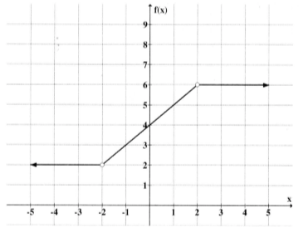
\includegraphics[width=0.5\textwidth]{./img/math_BAM_functions_1.png}
		\end{center}
		Use the graph to determine:
		\begin{enumerate}[topsep=0ex,itemsep=0ex,partopsep=1ex,parsep=1ex]
			\item[i)] The function $f(x)$
			\item[ii)] The domain and range of $f(x)$
		\end{enumerate}
		
		\item[(c)] Find the asymptotes and the intercepts of the function $f(x) = \frac{3x - 7}{x + 2}$ and then sketch its graph. 
	\end{enumerate}

\end{enumerate}












\subsection{Algebra}

\begin{enumerate}
	\item 
	\begin{enumerate}[topsep=0ex,itemsep=0ex,partopsep=1ex,parsep=1ex]
		\item[(a)] The roots of the polynomial equation $P(x) = x^3 - 7x^2 + Ax - 8$ form a geometric progression. Find, 
		\begin{enumerate}[topsep=0ex,itemsep=0ex,partopsep=1ex,parsep=1ex]
			\item[i)] The roots of the polynomial equation
			\item[ii)] The value of $A$
			\item[iii)] The abscissa at the turning points on the curve
		\end{enumerate}
		
		\item[(b)] Solve the following simultaneous equations by substitution method 
		\begin{center}
			$ \left\{ \begin{array}{l}
			xy = 16 \\
			x^2 + x^2 = 32
			\end{array} \right.$
		\end{center}
	\end{enumerate}
	
	\item
	\begin{enumerate}[topsep=0ex,itemsep=0ex,partopsep=1ex,parsep=1ex]
		\item[(a)] A series is given by $S_n = \sum_{r=1}^n (2r - 3)$,
		\begin{enumerate}[topsep=0ex,itemsep=0ex,partopsep=1ex,parsep=1ex]
			\item[i)] Determine the value of $S_{50}$ in series
			\item[ii)] Find the value of $n$ such that $S_{n} = 624$
		\end{enumerate}
		
		\item[(b)] Determine the values of $x$ and $y$ in the following simultaneous equations
		\begin{center}
			$ \left\{ \begin{array}{l}
			\log(x + y) = 1 \\
			\log_2{x} + 2\log_4{y} = 4
			\end{array} \right.$
		\end{center}
	\end{enumerate}

	\item
	\begin{enumerate}[topsep=0ex,itemsep=0ex,partopsep=1ex,parsep=1ex]
		\item[(a)] Given the series $-1 + 1 + 3, ...$
		\begin{enumerate}[topsep=0ex,itemsep=0ex,partopsep=1ex,parsep=1ex]
			\item[i)] Express it in the form $S_n = \sum_{r=1}^n f(r)$
			\item[ii)] Give one reason as to whether the series is an arithmetic or a geometric progression.
			\item[iii)] Determine the value of $n$ for which $S_n = 575$
		\end{enumerate}
		
		\item[(b)] If in a geometric progression, the second term exceeds the first term by 20 and the fourth term exceeds the second term by 15, find the possible values of the first term. 
	\end{enumerate}
\end{enumerate}











\input{./tex/Problems/Math_BAM/math_BAM_DIfferentiation.tex}
\subsection{Integration}

\begin{enumerate}
	\item 
	\begin{enumerate}[topsep=0ex,itemsep=0ex,partopsep=1ex,parsep=1ex]
		\item[(a)] If $f'(z) = ze^{x^2}$ and $f(0) = \frac{9}{2}$, find $f(z)$
		
		\item[(b)] 
		\begin{enumerate}[topsep=0ex,itemsep=0ex,partopsep=1ex,parsep=1ex]
			\item[i)] Calculate the area of the region bounded by the curve $y = x^2 + 3x - 18$ and the line $y = 0$
			\item[ii)] The marginal cost of producing $x$ units of a product are given by the equation $c'(x) = 0.6x^2 + 4x$. If the fixed cost is 30,000/=, find the cost function. 
		\end{enumerate}
	\end{enumerate}
	
	\item
	\begin{enumerate}[topsep=0ex,itemsep=0ex,partopsep=1ex,parsep=1ex]
		\item[(a)] Evaluate the following integrals: 
		\begin{center}
			$\int_0 ^{0.5\pi} \cos^3{x}$ $dx$
		\end{center} 
		
		\item[(b)] The slope of a curve at any point is defined by the equation $\frac{dy}{dx} = 3x - \frac{1}{x^2}$, where $x \neq 0$. Find the equation of the curve. 
		
		\item[(c)] The area bounded by the lines $y = mx$, $y = h$, $y = 0$, and $x = 0$ is rotated about the y-axis. If $x = r$ when $y = h$. Find the volume of the figure generated in terms of $h$ and $r$. 
	\end{enumerate}
	
	\item
	\begin{enumerate}[topsep=0ex,itemsep=0ex,partopsep=1ex,parsep=1ex]
		\item[(a)] Evaluate the following integrals
		\begin{enumerate}[topsep=0ex,itemsep=0ex,partopsep=1ex,parsep=1ex]
			\item[i)] $\int x(x+9)^{1/2}$ $dx$
			\item[ii)] $\int x \cos(5x + 9)$ $dx$
		\end{enumerate}
		
		\item[(b)] Given that $\int_2^4 \left(3x^2 - ax - \frac{16}{x^2}\right)$ $dx = 40$, find the values of the constant $a$. 
		
		\item[(c)] Sketch the graph of the curve $y = x^3 - 3x^2 + 2x$ and hence find the area bounded by the curve and the x-axis. 
	\end{enumerate}

\end{enumerate}













\subsection{Statistics}

\begin{enumerate}
	\item 
	\begin{enumerate}[topsep=0ex,itemsep=0ex,partopsep=1ex,parsep=1ex]
		\item[(a)] The number of motorcycle accidents which were recorded in one region in Tanzania for seven weeks during November and December 2013 were 14, 2, 12, 4, 10, 6, and 8. Find
		\begin{enumerate}[topsep=0ex,itemsep=0ex,partopsep=1ex,parsep=1ex]
			\item[i)] The mean number of accidents
			\item[ii)] The variance of the accidents
		\end{enumerate}
		
		\item[(b)] The table below shows the height of avocado trees in an orchard
		\begin{center}
			\begin{tabular}{|l|c|c|c|c|c|c|} \hline
				Height ($\times 10^{-1}$ m) & 2 - 6 & 7 - 11 & 12 - 16 & 17 - 21 & 22 - 26 & 27 - 31 \\ \hline
				Frequency & 12 & 14 & 18 & 15 & 4 & 8 \\ \hline
			\end{tabular}
		\end{center}
		\begin{enumerate}[topsep=0ex,itemsep=0ex,partopsep=1ex,parsep=1ex]
			\item[i)] Use the data to draw the histogram
			\item[ii)] Estimate the mode from the histogram in (b) i) above. 
		\end{enumerate}
	\end{enumerate}

	\item
	\begin{enumerate}[topsep=0ex,itemsep=0ex,partopsep=1ex,parsep=1ex]
		\item[(a)] Define the following terms as they are used in statistics:
		\begin{enumerate}[topsep=0ex,itemsep=0ex,partopsep=1ex,parsep=1ex]
			\item[i)] Range
			\item[ii)] Class size
		\end{enumerate}
		
		\item[(b)] The manager of Gold Mining Company recorded the number of absent workers in 52 working days as shown in the table below:
		\begin{center}
			\begin{tabular}{|l|c|c|c|c|c|} \hline
				Number of absent workers & 5 - 9 & 10 - 14 & 15 - 19 & 20 - 24 & 25 - 29 \\ \hline
				Frequency & 6 & 9 & 18 & 16 & 3 \\ \hline
			\end{tabular}
		\end{center}
		Use this data to construct the cumulative frequency curve.
		
		\item[(c)] The following data shows time in seconds which was recorded by a teacher in a swimming competition of students from Precious Beach High School.
		\begin{center}
			\begin{tabular}{ccccccccccc}
				32 & 31 & 27 & 30 & 29 & 27 & 25 & 29 & 26 & 26 & 32 \\
				32 & 25 & 31 & 31 & 27 & 24 & 26 & 26 & 32 & 33 & 28 \\
				26 & 33 & 24 & 28 & 32 & 29 & 32 & 24 & 31 & 27 & 30 \\
				31 & 25 & 29 & 25 & 27 & 30 & 26 \\
			\end{tabular}
		\end{center}
		\begin{enumerate}[topsep=0ex,itemsep=0ex,partopsep=1ex,parsep=1ex]
			\item[i)] Prepare the frequency distribution using the class intervals of 0-4, 5-9, etc. 
			\item[ii)] Determine the standard deviation. 
		\end{enumerate}
	\end{enumerate}
	
	\item The following were the scores obtained by 22 students from Sarawak Secondary School in a mathematics classroom test: 
	\begin{center}
		49, 64, 38, 60, 46, 64, 68, 42, 28, 68, 57, 63, 57, 63, 76, 51, 54, 66, 62, 63, 58, 59, 47, 55
	\end{center}
	\begin{enumerate}[topsep=0ex,itemsep=0ex,partopsep=1ex,parsep=1ex]
		\item[(a)] Summarize the scores in a frequency table with equal class intervals of size 5. Take the lowest limit to be 35. 
		\item[(b)] Find the mean score by using the data in part (a)
		\item[(c)] Find the interquartile range
		\item[(d)] How many students scored above the mean score?
	\end{enumerate}
	
\end{enumerate}













\subsection{Probability}

\begin{enumerate}
	\item
	\begin{enumerate}[topsep=0ex,itemsep=0ex,partopsep=1ex,parsep=1ex]
		\item[(a)] A fair coin is tossed once and the results are recorded, the a fair die is tossed.
		\begin{enumerate}[topsep=0ex,itemsep=0ex,partopsep=1ex,parsep=1ex]
			\item[i)] Draw a tree diagram to show the possible outcomes
			\item[ii)] Find the probability that, the outcome contains a head and even number.
		\end{enumerate}
		
		\item[(b)] Events X and Y are independent such that $P(X) = \frac{2}{3}$ and $P(X\cap Y)' = \frac{3}{4}$. Find, 
		\begin{enumerate}[topsep=0ex,itemsep=0ex,partopsep=1ex,parsep=1ex]
			\item[i)] $P(X/Y)$
			\item[ii)] $P(X \cup Y)$
		\end{enumerate}
	\end{enumerate}
	
	\item
	\begin{enumerate}[topsep=0ex,itemsep=0ex,partopsep=1ex,parsep=1ex]
		\item[(a)] If $P(n,4) = 42P(n,2)$
		\begin{enumerate}[topsep=0ex,itemsep=0ex,partopsep=1ex,parsep=1ex]
			\item[i)] Find $n$.
			\item[ii)] Evaluate $P(n,2)$ and $P(n,4)$.
		\end{enumerate}
		
		\item[(b)] Events A, B, and C are such that A and B are independent, while B and C are mutually exclusive. If $P(A) = \frac{1}{2}$, $P(B) = \frac{1}{4}$, and $P(C) = \frac{1}{3}$, find:
		\begin{enumerate}[topsep=0ex,itemsep=0ex,partopsep=1ex,parsep=1ex]
			\item[i)] $P(A \cap B)$
			\item[ii)] $P(A \cup B)$
			\item[iii)] $P(A \cup C)$
		\end{enumerate}
	\end{enumerate}	
	
	\item
	\begin{enumerate}[topsep=0ex,itemsep=0ex,partopsep=1ex,parsep=1ex]
		\item[(a)] If A and B are two events such that $P(A) = \frac{1}{4}$, $P(B) = \frac{1}{2}$ and $P(A \cap B) = \frac{1}{8}$, find $P(A \cup B)$ and $P(A' \cap B')$
		
		\item[(b)] A fair die was rolled and the events A and B were recorded as follows: A = \{1, 3, 5\} and B = \{2, 3, 4, 5\}. Find $P(A/B)$. 
		
		\item[(c)] In Section B of CSEE Basic Mathematics Examination each candidate has to choose and answer four out of six questions. How many choices are there for each candidate?
		
		\item[(d)] A box contains 4 ripe mangoes and 9 non-ripe mangoes. If two mangoes are randomly chosen from the box, find the probability that both will be ripe mangoes. 
	\end{enumerate}

\end{enumerate}











\subsection{Trigonometry}

\begin{enumerate}
	\item
	\begin{enumerate}[topsep=0ex,itemsep=0ex,partopsep=1ex,parsep=1ex]
		\item[(a)] Define the following terms
		\begin{enumerate}[topsep=0ex,itemsep=0ex,partopsep=1ex,parsep=1ex]
			\item[i)] Sine
			\item[ii)] Tangent
		\end{enumerate}
		
		\item[(b)] Evaluate $\tan15 \degree + \cot75 \degree$. Give the answer in simplest form.
		
		\item[(c)] Prove that $(1 - \cos{A})(1 + \cos{A}) = \sin{A}\tan{A}$
	\end{enumerate}

	\item
	\begin{enumerate}[topsep=0ex,itemsep=0ex,partopsep=1ex,parsep=1ex]
		\item[(a)] 
		\begin{enumerate}[topsep=0ex,itemsep=0ex,partopsep=1ex,parsep=1ex]
			\item[i)] Express $\sin3\theta$ in terms of $\sin\theta$
			\item[ii)] Show that $\sqrt{\frac{(1 - \cos{\phi})}{1 + \cos{\phi}}} = \csc{\phi} - \cot{\phi}$
		\end{enumerate}
		
		\item[(b)] Given the figure below,
		\vspace*{-7mm}
		\begin{center}
			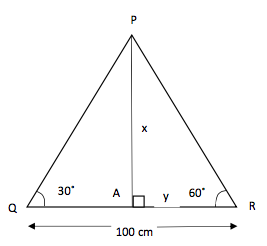
\includegraphics[width=0.45\textwidth]{./img/math_BAM_trig_1.png}
		\end{center}
		\begin{enumerate}[topsep=0ex,itemsep=0ex,partopsep=1ex,parsep=1ex]
			\item[i)] Determine the values of $x$ and $y$
			\item[ii)] Find $\sin(Q\hat{P}A)$
		\end{enumerate}
	\end{enumerate}
	
	\item
	\begin{enumerate}[topsep=0ex,itemsep=0ex,partopsep=1ex,parsep=1ex]
		\item[(a)] Without using a mathematical table or calculator, evaluate:
		\begin{enumerate}[topsep=0ex,itemsep=0ex,partopsep=1ex,parsep=1ex]
			\item[i)] $\cos(165 \degree)$
			\item[ii)] $\tan(A + B)$ given that A and B are acute angles having $\sin(A) = \frac{7}{25}$ and $\cos(B) = \frac{5}{13}$
		\end{enumerate}
		
		\item[(b)] 
		\begin{enumerate}[topsep=0ex,itemsep=0ex,partopsep=1ex,parsep=1ex]
			\item[i)] Find the values of $x$ that satisfy the equation $\sin{2x} + \cos{x} = 0$ for $0 \degree \leq x \leq 360 \degree$
			\item[ii)] Verify that the solution of the equation in part (b) i) can be obtained graphically by plotting the graph of $y= \sin{2x} + \cos{x}$ for $0 \degree \leq x \leq 360 \degree$
		\end{enumerate}
	\end{enumerate}

\end{enumerate}











\subsection{Exponents and Logarithms}

\begin{enumerate}
	\item 
	\begin{enumerate}[topsep=0ex,itemsep=0ex,partopsep=1ex,parsep=1ex]
		\item[(a)] Find $a$ if $2^{2a + 8} - 32(2^a) + 1 = 0$
		
		\item[(b)] If $2\log_8{N} = p$, $\log_2{2N} = q$, and $q - p = 4$, find $N$.
	\end{enumerate}
	
\end{enumerate}












\subsection{Matrices}

\begin{enumerate}
	\item
	\begin{enumerate}[topsep=0ex,itemsep=0ex,partopsep=1ex,parsep=1ex]
		\item[(a)] If $f(m) = m^2 - 4m - k$, find $f(N)$ when $k = \begin{pmatrix} 11 & -5 \\ -4 & 12 \end{pmatrix}$ and $N = \begin{pmatrix} 2 & 5 \\ 3 & 1 \end{pmatrix}$
		
		\item[(b)] Use Cramer's rule to solve the following system of linear equations
		\begin{center}
			$5x - 7y + z = 11$ \\
			$6x - 8y - z = 15$ \\
			$3x + 2y - 6z = 7$ 
		\end{center}
	\end{enumerate}
	
	\item Given the system of linear equations below
	\begin{center}
		$x + y + z = 7$ \\
		$x - y + 2z = 9$ \\
		$2x + y - z = 1$ 
	\end{center}
	\begin{enumerate}[topsep=0ex,itemsep=0ex,partopsep=1ex,parsep=1ex]
		\item[i)] Write the system of equations in matrix form
		\item[ii)] Find the determinant and the inverse of the matrix
		\item[iii)] Determine the values of $x$, $y$, and $z$
	\end{enumerate}
	
	\item 
	\begin{enumerate}[topsep=0ex,itemsep=0ex,partopsep=1ex,parsep=1ex]
		\item[(a)] Given:
		\begin{center}
		$A = \begin{pmatrix} 1 & 2 \\ 3 & 4 \\ -1 & 5 \end{pmatrix}$, $B = \begin{pmatrix} -2 & 3 & 4 \\ 3 & 2 & 1 \end{pmatrix}$, and $C = \begin{pmatrix} 3 & 5 \\ 1 & 2 \end{pmatrix}$
		\end{center}
		\begin{enumerate}[topsep=0ex,itemsep=0ex,partopsep=1ex,parsep=1ex]
			\item[i)] State with one reason as to whether the matrix operations $AB$, $BA$, and $BC$ are defined or not.
			\item[ii)] Find $2A + 3B^T$
		\end{enumerate}
		
		\item[(b)] Verify that $\begin{vmatrix} 1 & 1 & 1 \\ a & b & c \\ a^2 & b^2 & c^2 \end{vmatrix} = (a - b)(b - c)(c - a)$
		
		\item[(c)] If $D = \begin{pmatrix} a & -4 & -6 \\ -8 & 5 & 7 \\ -5 & 3 & 4 \end{pmatrix}$ is the inverse matrix $E = \begin{pmatrix} 1 & 2 & -2 \\ 3 & b & 1 \\ -1 & 1 & -3 \end{pmatrix}$, find the values of $a$ and $b$.
	\end{enumerate}

\end{enumerate}











\subsection{Linear Programming}

\begin{enumerate}
	\item 
	\begin{enumerate}[topsep=0ex,itemsep=0ex,partopsep=1ex,parsep=1ex]
		\item[(a)] Given the linear inequalities: $2y \leq 4x$, $x \leq 6$, $y \geq 2$, and $2x + 3y \leq 30$
		\begin{enumerate}[topsep=0ex,itemsep=0ex,partopsep=1ex,parsep=1ex]
			\item[i)] Draw the corresponding graph
			\item[ii)] List the corner points of the feasible region
		\end{enumerate}
		
		\item[(b)] The daily prophet obtained by Fruits Beverages Company in its business is given by the objective function $f(x,y) = 250x + 350y - 2200$ and the constraints:
		\begin{center}
			$x + y \geq 5.5$ \\
			$4x + 2y \geq 16$ \\
			$x + 2.5y \geq 9$ 
		\end{center}
		\begin{enumerate}[topsep=0ex,itemsep=0ex,partopsep=1ex,parsep=1ex]
			\item[i)] Represent the linear programming problem graphically
			\item[ii)] Determine the minimum and maximum profit of the company
		\end{enumerate}
	\end{enumerate}
	
	\item
	\begin{enumerate}[topsep=0ex,itemsep=0ex,partopsep=1ex,parsep=1ex]
		\item[(a)] Define the following terms:
		\begin{enumerate}[topsep=0ex,itemsep=0ex,partopsep=1ex,parsep=1ex]
			\item[i)] Linear programming
			\item[ii)] Constraints
		\end{enumerate}
		
		\item[(b)] A trader has 15,000, 9,000m and 1,920 units of ingredients X, Y, and Z for production of cakes and loaves. The requirements of units of a loaf of bread and a cake are indicated in the table below:
		\begin{center}
			\begin{tabular}{|l|c|c|c|} \hline
				\multirow{2}{*}{\textbf{Foodstuffs}} & \multicolumn{3}{|c|}{\textbf{Units}} \\ \cline{2-4}
				& X & Y & Z \\ \hline
				Bread & 25 & 10 & 30 \\ \hline
				Cake & 15 & 18 & 30 \\ \hline
			\end{tabular}
		\end{center}
		A loaf of bread is sold at 4,200/= shillings and a cake is sold at 2,000/= shillings.
		\begin{enumerate}[topsep=0ex,itemsep=0ex,partopsep=1ex,parsep=1ex]
			\item[i)] Sketch the graph to illustrate this information
			\item[ii)] What is the maximum amount of money obtained if both cakes and loaves of bread must be prepared?
			\item[iii)] What should the trader do to obtain that maximum profit?
		\end{enumerate}	
	\end{enumerate}

	\item
	\begin{enumerate}[topsep=0ex,itemsep=0ex,partopsep=1ex,parsep=1ex]
		\item[(a)] Mr. Taramise owns 480 acres of land on which he grows either maize or beans during the farming period. He normally expects a profit of Tshs 40,000/= per acres on maize and Tshs 30,000/= per acre on beans and he has 800 hours of labor available. If maize requires 2 hours per acre to raise and beans require 1 hour per acre to raise, find how many acres of maize and beans he should plant to get maximum profit. 
	\end{enumerate}

\end{enumerate}













%\section{Advance Level - Applied Mathematics (AM) Topics}
%\input{./tex/Problems/Math_AM/math_AM_.tex}

\section{Form VI NECTA Applied Mathematics (AM) Exam - 2017}

%%%%%%%% Physics %%%%%%%%%
\chapter{Physics}
% Format
\section{NECTA Physics Exam Format}
\label{sec:physics-format}

%%%%%%%%%%%%%%%%%%%%%%%%%%%%%
%-----------------------------Form II------------------------------------
%%%%%%%%%%%%%%%%%%%%%%%%%%%%%
\subsection{Form II}
\noindent The following format for the Form Two National Assessment (FTNA) is based on the revised version of the Physics Syllabus for Ordinary Secondary Education of 2007. The exam is intended to assess the competences acquired by the students after two years of study. The following information was taken from The National Examinations Council of Tanzania - Form Two National Assessment Formats %CITE!!!!!!!!!!!!!!!!!!

\subsubsection{General Objectives}
\noindent The general objectives of the Physics assessment are to test students' ability to:
\begin{enumerate}[topsep=1ex,itemsep=0ex,partopsep=1ex,parsep=1ex]
	\item Demonstrate laboratory practice and safety
	\item Develop skills on basic principles of scientific investigation
	\item Develop skills for making physical measurements
	\item Recognize behavior and properties of matter
	\item Understand concepts and principles of magnetism and electricity
	\item Comprehend the laws of motion
	\item Understand principles of simple machines
	\item Develop knowledge on sustainable energy for environmental conservation
\end{enumerate}

\subsubsection{General Competences}
\noindent The FTNA will specifically test the students' ability to:
\begin{enumerate}[topsep=1ex,itemsep=0ex,partopsep=1ex,parsep=1ex]
	\item Practice safety rules in daily life
	\item Apply basic principles of scientific investigation
	\item Make appropriate measurements of physical quantities
	\item Use scientific skills to identify nature and properties of matter
	\item Apply electricity and magnetism knowledge in daily life
	\item Apply laws of motion in dealing with moving objects
	\item Use simple machines to simplify work
	\item Practice environmental conservation by adopting appropriate sustainable energy sources
\end{enumerate}

\subsubsection{Assessment Rubric}
\noindent The assessment consists of \textbf{one (1)} theory paper. The duration of the exam is \textbf{2 hours and 30 minutes}. The paper consists of \textbf{ten (10)} questions categorized into sections A, B, and C. The students are required to attempt \textbf{all} questions from \textbf{all} sections. 
\begin{enumerate}
	\item \textbf{Section A} \\
	This section has \textbf{three (3)} objective questions. This section weighs a total of \textbf{thirty (30)} marks.
	\begin{enumerate}
		\item Question 1 is composed of 20 multiple choice items derived from various topics (20 marks)
		\item Question 2 is composed of 5 matching items (5 marks)
		\item Question 3 is composed of 5 filling in the blank items derived from various topics (5 marks)
	\end{enumerate}
	
	\item \textbf{Section B} \\
	This section has \textbf{five (5)} short answer questions (10 marks each). This section weighs a total of \textbf{fifty (50)} marks.
	
	\item \textbf{Section C} \\
	This section has \textbf{two (2)} questions (10 marks each). The questions are aimed at assessing students' knowledge and skills in drawing and management of Physics apparati and simple technological devices in everyday life. This section weighs a total of \textbf{twenty (20)} marks. 
\end{enumerate}

\subsubsection{Assessment Topics}
\noindent The following table shows the topics assessed in the FTNA as well as the percentage they have appeared in past examinations. 
\begin{center}
	\begin{tabular}{|c|l|c|c|} \hline
		Form & \multicolumn{1}{|c|}{Topic} & Percentage [\%] & Total Percentage [\%] \\ \hline
		\multirow{9}{*}{I} 	& Introduction to Physics 					& 1.25 & \multirow{9}{*}{47.76}	\\ \cline{2-3}
						& Introduction to Laboratory Practice 		& 0.97 & \\ \cline{2-3}
						& Measurements						& 10.58 & \\ \cline{2-3}
						& Forces 								& 4.32 & \\ \cline{2-3}
						& Archimedes Principle and Law of Floatation 	& 3.90 & \\ \cline{2-3}
						& Structure and Properties of Matter 			& 7.52 & \\ \cline{2-3}
						& Pressure							& 4.32 & \\ \cline{2-3}
						& Work, Energy and Power				& 6.82 & \\ \cline{2-3}
						& Light 								& 8.08 & \\ \hline
		\multirow{9}{*}{II} 	& Static Electricity	 					& 4.87 & \multirow{9}{*}{43.02} \\ \cline{2-3}
						& Current Electricity				 		& 8.08 & \\ \cline{2-3}
						& Magentism							& 5.15 & \\ \cline{2-3}
						& Forces in Equilibrium					& 3.90 & \\ \cline{2-3}
						& Simple Machines					 	& 7.24 & \\ \cline{2-3}
						& Motion in Straight Lines		 			& 5.01 & \\ \cline{2-3}
						& Newton's Laws of Motion				& 3.76 & \\ \cline{2-3}
						& Temperature							& 3.34 & \\ \cline{2-3}
						& Sustainable Energy Sources				& 1.67 & \\ \hline
	\end{tabular}
\end{center}

%%%%%%%%%%%%%%%%%%%%%%%%%%%%%
%-----------------------------Form IV------------------------------------
%%%%%%%%%%%%%%%%%%%%%%%%%%%%%
\subsection{Form IV}
\noindent The following format for the Form Four Certificate of Secondary Education (CSEE) is based on the revised version of the Physics Syllabus for Ordinary Secondary Education of 2007. The exam is intended to assess the competences acquired by the students after four years of study. The following information was taken from The National Examinations Council of Tanzania - Certificate of Secondary Education Examination Formats %CITE!!!!!!!!!!!!!!!!!!

\subsubsection{General Objectives}
\noindent The general objectives of the Physics examination are to test students' ability to:
\begin{enumerate}[topsep=1ex,itemsep=0ex,partopsep=1ex,parsep=1ex]
	\item Develop knowledge of concepts, laws, theories and principles of Physics
	\item Use procedures of scientific investigation
	\item Use scientific principles on conservation and suitable use of the environment
	\item Demonstrate manipulative skills to manage various technological appliances
	\item Develop the language of communication in physics
\end{enumerate}

\subsubsection{General Competences}
\noindent The CSEE will specifically test the students' ability to:
\begin{enumerate}[topsep=1ex,itemsep=0ex,partopsep=1ex,parsep=1ex]
	\item Use Physics knowledge, principles and concepts in daily life
	\item Demonstrate scientific methods in solving problems in daily life
	\item Demonstrate technological skills in conservation and sustainable use of the environment
	\item Manage simple technological appliances
	\item Use the language of Physics in communication
\end{enumerate}

\subsubsection{Examination Rubric}
\noindent The examination consists of \textbf{two (2)} papers. The first paper focuses on theory while the second focuses on practicals. This section will discuss the format for the Physics theory paper. To see the format of the Physics practical paper, please refer to Section \ref{phy-practical-format}. \\

\noindent The duration of the theory exam is \textbf{3 hours}. The paper consists of \textbf{eleven (11)} questions categorized into sections A, B, and C. The students are required to attempt \textbf{all} questions from sections A and B and \textbf{one} question from section C. 
\begin{enumerate}
	\item \textbf{Section A} \\
	This section has \textbf{three (3)} objective questions. This section weighs a total of \textbf{thirty (30)} marks.
	\begin{enumerate}
		\item Question 1 is composed of 10 multiple choice items derived from various topics (10 marks)
		\item Question 2 is composed of 10 matching items (10 marks)
		\item Question 3 is composed of 10 filling in the blank items derived from various topics (10 marks)
	\end{enumerate}
	
	\item \textbf{Section B} \\
	This section has \textbf{six (6)} long answer questions (10 marks each). This section weighs a total of \textbf{sixty (60)} marks.
	
	\item \textbf{Section C} \\
	This section has \textbf{two (2)} questions (10 marks each). The questions are aimed at assessing students' knowledge and skills in drawing and management of Physics apparati and simple technological devices in everyday life. This section weighs a total of \textbf{ten (10)} marks. 
\end{enumerate}


\subsubsection{Examination Topics}
\noindent The following table shows the topics assessed in the CSEE as well as the percentage they have appeared in past examinations. 
\begin{center}
	\begin{longtable}{|c|l|c|c|} 
	
		\hline Form & \multicolumn{1}{|c|}{Topic} & Percentage [\%] & Total Percentage [\%] \\ \hline
		\endfirsthead
		
		\hline Form & \multicolumn{1}{|c|}{Topic} & Percentage [\%] & Total Percentage [\%] \\ \hline
		\endhead
		
		\multirow{9}{*}{I} 	& Introduction to Physics 					& 0.00 & \multirow{9}{*}{14.14} 	\\ \cline{2-3}
						& Introduction to Laboratory Practice 		& 0.00 & 					\\ \cline{2-3}
						& Measurements						& 3.08 & 					\\ \cline{2-3}
						& Forces 								& 1.03 & 					\\ \cline{2-3}
						& Archimedes Principle and Law of Floatation 	& 1.94 & 					\\ \cline{2-3}
						& Structure and Properties of Matter 			& 1.60 & 					\\ \cline{2-3}
						& Pressure							& 2.05 & 					\\ \cline{2-3}
						& Work, Energy and Power				& 2.74 & 					\\ \cline{2-3}
						& Light 								& 1.71 & 					\\ \hline
		\multirow{9}{*}{II} 	& Static Electricity	 					& 3.42 & \multirow{9}{*}{21.32}	\\ \cline{2-3}
						& Current Electricity				 		& 2.17 & 					\\ \cline{2-3}
						& Magentism							& 2.39 & 					\\ \cline{2-3}
						& Forces in Equilibrium					& 2.85 & 					\\ \cline{2-3}
						& Simple Machines					 	& 1.94 & 					\\ \cline{2-3}
						& Motion in Straight Lines		 			& 3.31 & 					\\ \cline{2-3}
						& Newton's Laws of Motion				& 3.19 & 					\\ \cline{2-3}
						& Temperature							& 1.37 & 					\\ \cline{2-3}
						& Sustainable Energy Sources				& 0.68 & 					\\ \hline
		\multirow{9}{*}{III}	& Application of Vectors					& 0.80 & \multirow{9}{*}{28.96}	\\ \cline{2-3}
						& Friction								& 0.23 & 					\\ \cline{2-3}
						& Light								& 6.73 & 					\\ \cline{2-3}
						& Optical Instruments					& 0.80 & 					\\ \cline{2-3}
						& Thermal Expansion					& 3.76 & 					\\ \cline{2-3}
						& Transfer of Thermal Heat				& 1.14 & 					\\ \cline{2-3}
						& Measurement of Thermal Energy			& 3.31 & 					\\ \cline{2-3}
						& Vapour and Humidity					& 1.25 & 					\\ \cline{2-3}
						& Current Electricity 						& 10.95 & 					\\ \hline
		\multirow{7}{*}{IV}	& Waves								& 6.61 & \multirow{7}{*}{35.58}	\\ \cline{2-3}
						& Electromagnetism						& 4.45 & 					\\ \cline{2-3}
						& Radioactivity							& 8.44 & 					\\ \cline{2-3}
						& Thermionic Emission					& 3.42 & 					\\ \cline{2-3}
						& Electronics							& 6.16 & 					\\ \cline{2-3}
						& Astronomy							& 4.56 & 					\\ \cline{2-3}
						& Geophysics							& 1.94 & 					\\ \hline
	\end{longtable}
\end{center}



\vspace*{-10mm}
% Form I
\section{Form I Topics}
%\subsection{Introduction to Physics}















\subsection{Introduction to Laboratory Practice}

\begin{enumerate}
	\item Which of the following scientific statements need to be proved through scientific research?
	\begin{enumerate}[topsep=0ex,itemsep=0ex,partopsep=1ex,parsep=1ex]
		\item[(A)] Hypothesis
		\item[(B)] Principle
		\item[(C)] Conclusion
		\item[(D)] Proposal
		\item[(E)] Measurement
	\end{enumerate}
\end{enumerate}











\subsection{Measurement}

\begin{enumerate}
	\item In laboratory, the diameter of a piece of wire can accurately be measured by:
	\begin{enumerate}[topsep=0ex,itemsep=0ex,partopsep=1ex,parsep=1ex]
		\item[(A)] Vernier caliper
		\item[(B)] Micrometer screw gauge
		\item[(C)] Engineer's caliper
		\item[(D)] Rate meter
		\item[(E)] Thread wound round it once
	\end{enumerate}

	\item An auto mechanic wants to measure the diameter of a wire to the nearest 0.001 cm. Which of the following instruments can be used?
	\begin{enumerate}[topsep=0ex,itemsep=0ex,partopsep=1ex,parsep=1ex]
		\item[(A)] Venier caliper
		\item[(B)] Micrometer screw gauge
		\item[(C)] Metre rule
		\item[(D)] Pair of compasses
		\item[(E)] Engineer's caliper
	\end{enumerate}
	
	\item Each scientific instrument is limited in accuracy, what is the shortest length that can be accurately recorded or measured by a meter rule?
	\begin{enumerate}[topsep=0ex,itemsep=0ex,partopsep=1ex,parsep=1ex]
		\item[(A)] 0.02 mm
		\item[(B)] 0.2 mm
		\item[(C)] 0.02cm
		\item[(D)] 0.2m
	\end{enumerate}
	
	\item 
	\begin{enumerate}[topsep=0ex,itemsep=0ex,partopsep=1ex,parsep=1ex]
		\item[i)] What effect does an increase in temperature have on the density of most liquids?
		\item[ii)] Explain the procedure for using methylated spirit, water and a pendulum bob to find the relative density of spirit.
	\end{enumerate}
	
	\item
	\begin{enumerate}[topsep=0ex,itemsep=0ex,partopsep=1ex,parsep=1ex]
		\item[i)] Define relative density
		\item[ii)] In an experiment using Hare's apparatus, the lengths of methanol and water columns were found to be 16 cm and 12.80 cm respectively. Find the relative density of methanol. 
		\item[iii)] If the length of methanol column was altered to 21.50 cm what would be the new height of the water column?
	\end{enumerate}
	
	\item The mass of 1.5 litres of water is \rule{1.5cm}{0.15mm} kg.
	\begin{enumerate}[topsep=0ex,itemsep=0ex,partopsep=1ex,parsep=1ex]
		\item[(A)] 1500
		\item[(B)] 150
		\item[(C)] 15
		\item[(D)] 1.5
		\item[(E)] 0.15
	\end{enumerate}

\end{enumerate}












\subsection{Force}
\subsection{Archimedes' Principle and Law of Floatation}
\subsection{Structure and Properties of Matter}
\subsection{Pressure}
\subsection{Work, Energy and Power}
\subsection{Light}

% Form II
\section{Form II Topics}
\subsection{Static Electricity}
\subsection{Current Electricity}
\subsection{Magnetism}
\subsection{Forces in Equilibrium}
\subsection{Simple Machines}
\subsection{Motion in a Straight Line}
\subsection{Newton's Law of Motion}
\subsection{Temperature}
\subsection{Sustainable Energy Sources}

% Form III
\section{Form III Topics}
\subsection{Applications of Vectors}
\subsection{Friction}
\subsection{Light}
\subsection{Optical Instruments}
\subsection{Thermal Expansion}
\subsection{Transfer of Thermal Energy}
\subsection{Measurement of Thermal Energy}
\subsection{Vapour and Humidity}
\subsection{Thermal Current Electricity}

% Form IV
\section{Form IV Topics}
\subsection{Waves}
\subsection{Electromagnetism}
\subsection{Radioactivity}
\subsection{Thermionic Emission}
\subsection{Electronics}
\subsection{Elementary Astronomy}
\subsection{Geophysics}

% Form V and VI
%\section{Advance Level Topics}
%\subsection{Measurement}
%\subsection{Mechanics}
%\subsection{Fluid Dynamics}
%\subsection{Properties of Matter}
%\subsection{Heat}
%\subsection{Vibrations and Waves}
%\subsection{Electrostatics}

%\subsection{Electromagnetism}
%\subsection{Current Electricity}
%\subsection{Electronics}

\section{Form VI NECTA Physics Exam - 2017} 

%--------------------------------------------------------------------------------------------------
\part{NECTA Practicals}
%%%%%%%% Biology %%%%%%%%%
\chapter{Biology}
%\section{Introduction to Biology Practicals} 

\subsection{Format}
The theory portion of the Biology exam comprises 100 marks, while the practical carries 50 marks. A student's final grade for Biology is thus found by taking her total marks from both exams out of 150.

As of now, the Biology practical has 2 questions and students must answer \textbf{both}. Question 1 can come from any of the following topics: Nutrition, Movement, Transport of Living Things, Respiration, Reproduction, Coordination, Regulation or Growth. Question 2 is on Classification of Living Things. Each question is worth 25 marks, and students have 2$\frac{1}{2}$ hours to complete the exam.

\paragraph{Note} This information is current as of the time of publication of this manual. Updated information may be obtained by contacting the Ministry of Education. 

\subsection{NECTA Advance Instructions for Teachers}

There are two sets of advance instructions. One set of advance instruction are given to teachers at least one month before the date of the exam. These instructions contain the list of specimen, apparatus, and other materials required for setting up the Biology practical questions. The instructions also suggest how many specimen to acquire for each candidate or group of candidates. It is imperative that the collection and storage of specimen for the practical be kept confidential.

The second set of instructions should be given 24 hours before the time of the practical. It includes how to label each specimen and which materials should be given to each candidate (or shared among candidates).

Usually if the instructions include a scalpel of some sort, this means students will be required to do some form of dissection. In most cases, the dissection is of a maize seed or bean to show whether is it a monocotyledon or dicotyledon. If the advance instructions include any form of glass apparatus or test tubes, there will most likely be a question on food tests.

\subsection{Common Practicals}
\begin{description}
\item[Food Tests]{test a food solution for starch, sugars, fats, and protein}
\item[Classification]{name and classify specimens, then answer questions about their characteristics}
\item[Respiration]{use lime water to test air from the lungs for carbon dioxide}
\item[Transport]{investigate osmosis by placing leaf petioles or pieces of raw potato in solutions of different solute concentrations}
\item[Photosynthesis]{test a variegated leaf for starch to prove that chlorophyll is necessary for photosynthesis}
\item[Coordination]{students look at themselves in the mirror and answer questions about the sense organs they see}
\item[Movement]{name bones and answer questions about their structure and position in the body}
\end{description}

\paragraph{Note} These are the most common practicals, but they are not necessarily the only practicals that can occur on the national exam. Food tests and Classification are by far the most common, but there are many eligible topics. Be sure to regularly look through \nameref{cha:past-papers-bio} (p.~\pageref{cha:past-papers-bio}) to get an idea of the kind of questions that can occur.

%==============================================================================
\section{Food Tests} \index{Practicals! Biology! food tests} \index{Food tests}

In this practical, students test a solution of unknown food substances for starch, protein, reducing sugars, non-reducing sugars, and lipids. They record their procedure, observation, and conclusions, then answer questions about nutrition and the digestive system.\\

\noindent This section contains the following:
\begin{itemize}
\item{Preparation of Chemical Solutions}
\item{Preparation of Food Solutions}
\item{Performing the Food Tests}
\item{Examination Room}
\item{Student Report}
\item{Sample Food Test Practical}
%\item{Sample Food Test Solutions}
\end{itemize}

\subsection{Preparation of Chemical Solutions}
Always make sure the chemicals work before performing the food tests with students.

\subsubsection{Benedict's Solution} \index{Benedict's solution! for food tests}
This solution can be bought at a chemical store already prepared or you can make it yourself.\\

\textbf{Using Sodium Carbonate:}
\begin{itemize*}
\item Add about 1 L of water to a plastic bottle.
\item Add 5 spoons of sodium carbonate (NaCO$_3$).
\item Add 3 spoons of citric acid.
\item Add one spoon of copper sulphate.
\end{itemize*}

\textbf{Using Bicarbonate of Soda:}
\begin{itemize*}
\item Add 1 L of water to a cooking pot.
\item Add a box (70 g) of bicarbonate of soda.
\item Boil the mixture for 5-10 minutes. This makes sodium carbonate.
\item Let cool and transfer to a plastic water bottle.
\item Add 3 spoons of citric acid.
\item Add one spoon of copper sulphate. Cap and shake to mix.
\end{itemize*}

\noindent Label as: BENEDICT'S SOLUTION FOR FOOD TESTS

\noindent The solution may be stored in any plastic or glass bottle and will keep indefinitely.

\subsubsection{Copper (II) Sulphate} \index{Copper sulphate! for food tests}
\begin{itemize*}
\item Add one spoon of copper (II) sulphate to a 1.5 L bottle.
\item Add 1 L of water and shake until chemicals are fully dissolved.
\end{itemize*}

\noindent Label as: 1\% COPPER (II) SULPHATE SOLUTION FOR FOOD TESTS

\noindent The solution may be stored in any plastic or glass bottle and will keep indefinitely.

\subsubsection{Iodine Solution} \index{Iodine solution! for food tests}
Make sure to use iodine tincture from a pharmacy. The tincture must not contain ethanol\slash alcohol\slash spirit.

\begin{itemize*}
\item Add 1 part iodine tincture to 10 parts water. Example: In a 500 mL bottle, add 40 mL iodine tincture, then and 400 mL of water.
\item Cap the bottle and shake.
\end{itemize*}

\noindent Label as: IODINE SOLUTION FOR FOOD TESTS

\noindent The solution may be stored in any plastic or glass bottle and will keep indefinitely.

\subsubsection{Dilute NaOH} \index{Sodium hydroxide! for food tests}
\begin{itemize*}
\item Using a PLASTIC teaspoon, add one level teaspoon of NaOH to a 500 mL water bottle. Caustic soda (NaOH) reacts with metal. DO NOT TOUCH.

\emph{SAFETY NOTE: Prepare about 100 mL of citric acid or ethanoic acid solution to neutralize sodium hydroxide spills on skin or lab tables. One spoon of citric acid in 100 mL of water is suitable. Ethanoic acid solutions are sold in stores as vinegar.}

\item Add 250 mL of water.

\emph{SAFETY NOTE: This reaction can cause the solution to become very warm. Avoid chemical burns by wearing gloves.}

\item Cap well and shake. This makes 1 M sodium hydroxide solution.
\end{itemize*}

\noindent Label as: 1 M SODIUM HYDROXIDE SOLUTION FOR FOOD TESTS (CORROSIVE)

\noindent The solution will react with carbon dioxide in the air if not well sealed. Do not store in glass bottles with glass stoppers as these will stick. The solution may be stored in plastic bottles indefinitely.


\subsubsection{Dilute Acid} \index{Hydrochloric acid! for food tests} \index{Citric acid! for food tests}
Your school may have dilute hydrochloric acid or you may have to make it yourself.\\

\textbf{Using Hydrochloric Acid (HCl):}
\begin{itemize*}
\item Add 1 part HCl to 9 parts water. Example: In a 1.5 L water bottle, add 900 mL of water, then add 100 mL of HCl.
\item Shake well.
\end{itemize*}

\textbf{Using Citric Acid:}
\begin{itemize*}
\item Add 500 mL of water to a 1 or 1.5 L water bottle.
\item Add 5 spoons of citric acid.
\item Cap well and shake. This makes 0.5 M citric acid.
\end{itemize*}

\noindent Label as: 0.5 M CITRIC ACID FOR FOOD TESTS

\noindent The solution may be stored in any plastic or glass bottle and will keep indefinitely.

\subsubsection{Sudan III Solution} \index{Sudan III solution! for food tests}
Using Sudan III solution takes a long time to show results. It may be replaced by iodine tincture solution for the lipids test.

\begin{itemize*}
\item Combine 0.5 g of Sudan III powder with 100 mL of 70\% ethanol solution (30 mL water and 70 mL ethanol).
\item Place the solution in a warm water bath to help the Sudan III dissolve.
\item Filter to remove any remaining solid.
\end{itemize*}

\noindent Label as: SUDAN III SOLUTION FOR FOOD TESTS

\noindent The solution may be stored in any plastic or glass bottle and will keep indefinitely.


\subsection{Preparation of Food Solutions}
For the NECTA and mock exams you may have to set up the food test solutions. The instructions will tell you which ones you'll need to prepare in order to make `Solution X.' Solution X consists of a mixture of at least 3 of the different food substances and is given to each student in at least 3 test tubes. Make sure food solutions are well-dissolved and colorless so that students don't know what is in the mixture. You don't need to measure the ingredients, but make sure to test the solutions before the practical.

\subsubsection{Reducing sugar}
Use glucose powder and dissolve in water. Make sure the substance is fully dissolved so that students don't know what is in the mixture.

\subsubsection{Non-reducing sugar}
Use sugar and dissolve in water. Make sure the substance is fully dissolved so that students don't know what is in the mixture.

\subsubsection{Lipids}
Mix sunflower oil with water. Shake immediately before use. Sunflower oil is best since it is liquid at room temperature.

\subsubsection{Protein}
Mix an egg white with water.

\subsubsection{Starch}
Save the water you use to boil potatoes, rice, or pasta. Make sure to remove the bits of food. You can also just mix flour in water, but it would be obvious.


\subsection{Performing the Food Tests}

\subsubsection{Reducing Sugars Test}
\begin{itemize*}
\item Add a small amount of Benedict's solution to the food solution. 
\item Boil the solution and allow it to cool. Observe the colour changes from blue to green, yellow, then deep orange\slash brick red precipitate if reducing sugars are present.
\end{itemize*}
Always do the reducing sugars test first because a non-reducing sugar will always test positive for a reducing sugar.

\subsubsection{Non-reducing Sugars Test}
\begin{itemize*}
\item Add a small amount of dilute acid (HCl) to the solution. 
\item Boil the solution for about 30 seconds and allow it to cool. 
\item Add a small amount of NaOH to the solution and shake.
\item Add a small amount of Benedict's solution and boil. 
\item Allow the solution to cool and observe as the solution changes from green to yellow, then to deep orange\slash brick red precipitate if non-reducing sugars are present.
\end{itemize*}

\subsubsection{Lipids Test}
\begin{itemize*}
\item Add a small amount of Sudan III or iodine solution to the food solution and shake. 
\item A red ring will form at the top of the test tube if lipids are present.
\end{itemize*}
Using Sudan III colours the whole solution red whether it contains lipids or not. Use iodine solution to get a more distinct result.

\subsubsection{Protein Test}
\begin{itemize*}
\item Add an \emph{equal} amount of sodium hydroxide (NaOH) to the solution and shake. 
\item Add a small amount of copper (II) sulphate to the solution and shake.
\item Observe the solution turn violet\slash purple in colour if protein is present.
\end{itemize*}

\subsubsection{Starch Test}
\begin{itemize*}
\item Add a small amount of iodine solution to the food solution.
\item Observe the solution turn blue-black in colour if starch is present.
\end{itemize*}


\subsection{Examination Room}
The NECTA practical exam is done in the school's lab or any other suitable room. Heat sources (jiko, etc.) should be spread evenly in the exam room so that students don't have to go far to heat their test tubes; this also cuts down on cheating. Spread students out and distribute supplies as you see fit.\\

\noindent \textbf{Each student gets:}
\begin{itemize*}
\item[-] 3 or more test tubes (to carry out 5 tests)
\item[-] A beaker containing Solution X
\item[-] A test tube rack (or a cut out water bottle with sand to hold the tubes)*
\end{itemize*}
* Students may share the racks, but shouldn't share the cut out bottles\\

\noindent \textbf{Each station should have:}
\begin{itemize*}
\item[-] Copper II sulphate
\item[-] Water
\item[-] Dilute acid (HCl, etc.)
\item[-] Dilute base (sodium hydroxide)
\item[-] Iodine solution
\item[-] Sudan III solution (can be replaced by iodine solution)
\item[-] Benedict's solution
\end{itemize*}

\subsection{Student Report}
Food test data is recorded in a table containing four columns: Test for, Procedure, Observation and Inference.

Students should write the Procedure using the passive voice in the past tense. For example, ``A small amount of Benedict's solution was added to the solution. Then the solution was boiled and allowed to cool.''

In the Observation column, the student should write what they observed using the past tense and passive voice. For example, ``A violet colour was observed.''

In the Inferences column, the students should write what they saw in the past tense and passive voice. For example, ``Reducing sugars were not (or were) present.''

Note that every column is worth marks on the exam. Even if students fail to do the food tests correctly, they can still get marks for writing what they are testing for and what the procedure should be.

An example of a completed food test results table is given below. Assume the solution contains proteins, reducing sugars, non-reducing sugars and starch.

\begin{center}
\begin{tabular}{|p{3cm}|p{5cm}|p{3cm}|p{3cm}|} \hline
\multicolumn{1}{|c|}{\textbf{Food Tested}}&\multicolumn{1}{c|}{\textbf{Procedure}}&\multicolumn{1}{c|}{\textbf{Observation}}&\multicolumn{1}{c|}{\textbf{Inference}} \\ \hline
Lipids & A few drops of Sudan III solution (or iodine solution) were added to solution X. The solution was shaken and allowed to stand. & A red ring did not form at the surface. & Lipids were not present.\\ \hline
Proteins & An equal amount of NaOH was added to solution X and shaken. A few drops of copper (II) sulphate were added to solution X and shaken again. & A violet colour was observed. & Proteins were present.\\ \hline
Reducing sugars & A small amount of Benedict's solution  was added to solution X. The solution was heated and allowed to cool. & A brick red precipitate was observed. & Reducing sugars were present.\\ \hline
Non-reducing sugars & A small amount of dilute acid was added to solution X. The solution was heated and allowed to cool. Then a small amount of NaOH solution was added, and the solution was shaken. Finally, a small amount of Benedict’s solution was added. The solution was boiled and let cool. & The solution changed from green to yellow, then to a deep orange\slash brick red precipitate. & Non-reducing sugars were present.\\ \hline
Starch & A few drops of iodine solution were added to solution X and shaken. & A blue-black colour was observed. & Starch was present.\\ \hline
\end{tabular}
\end{center}

\subsection{Sample Food Test Practical}
You have been provided with solution \textbf{B}. 

\begin{enumerate}
\item[(a)] Identify the food substances present in solution \textbf{B} by using the reagents provided. Tabulate your work as shown in the following Table:

\begin{center}
\begin{tabular}{|p{3cm}|p{3cm}|p{3cm}|p{3cm}|} \hline
\multicolumn{1}{|c|}{\textbf{Food Tested}}&\multicolumn{1}{c|}{\textbf{Procedure}}&\multicolumn{1}{c|}{\textbf{Observation}}&\multicolumn{1}{c|}{\textbf{Inference}} \\ \hline
&&& \\
&&& \\
&&& \\
&&& \\ \hline
\end{tabular} \\[10pt]
\end{center}

\item[(b)] For each food substance identified in 1(a);
\begin{enumerate}
\item[(i)] Name two common sources.
\item[(ii)] State their role in the body of human being.
\end{enumerate}
\item[(c)] The digestion of one of the identified food substance in 1(a) starts in the mouth.
\begin{enumerate}
\item[(i)] Name this food substance.
\item[(ii)] Identify the enzyme responsible for its digestion in the mouth.
\end{enumerate}
\item[(d)] The digestive system of human being has several parts.
\begin{enumerate}
\item[(i)] Name the part of digestive system in which most of digestion and absorption of food takes place.
\item[(ii)] Explain how the named part in (d) (i) is adapted for absorption of digested food substances.
\end{enumerate}
\end{enumerate}

\textbf{Additional Food Test Questions:}
See \nameref{cha:past-papers-bio} (p.~\pageref{cha:past-papers-bio}) for additional food test questions.

%\begin{enumerate*}
%\item[(e)] What is the function of each of the food substances in solution \textbf{B} to human beings? 
%\item[(f)] For each food substance identified, name the enzyme and end product of digestion 
%taking place in the:\\
%\begin{enumerate*}
%\item[(i)] Stomach
%\item[(ii)] Duodenum
%\end{enumerate*}
%\item[(g)] What deficiency diseases are caused by a lack of the identified food substances?
%\end{enumerate*}


%\subsection{Sample Food Test Solutions}



%\section{Food Tests}
%
%In this practical, students test a solution of unknown food substances for starch, protein, reducing sugars, non-reducing sugars, and fats\slash oils. They record their procedure, observation, and conclusions, then answer questions about nutrition and the digestive system.
%
%This section contains the following:
%\begin{itemize}
%\item{Preparation of test solutions}
%\item{Preparation of food solutions}
%\item{How to carry out food tests}
%\item{How to write a report}
%\item{Sample practical with solutions}
%\end{itemize}
%
%\subsection{Test for Starch}
%
%\subsubsection{Materials}
%\begin{itemize}
%\item{iodine tincture from the pharmacy (any brand)}
%\item{tap or clean river water}
%\end{itemize}
%
%\subsubsection{Procedure to make 400~mL}
%\begin{enumerate}
%\item{40~mL of iodine tincture to a 500~mL plastic water bottle.}
%\item{Add about 400~mL of water.}
%\item{Cap the bottle and shake.}
%\item{Use a permanent pen to label the bottle:\\
%IODINE SOLUTION FOR FOOD TESTS}
%
%The solution may be stored in any plastic or glass bottle and will keep indefinitely.
%\end{enumerate}
%
%\subsection{Test for protein}
%
%The best test for protein is the Biuret test. This requires two solutions: 1\% \ce{CuSO4} and 1~M \ce{NaOH}.
%
%\subsubsection{Materials}
%\begin{itemize}
%\item{copper sulfate}
%\item{sodium hydroxide}
%\item{tap or clean river water}
%\end{itemize}
%
%\subsubsection{Procedure to make 1~L copper sulfate solution}
%\begin{enumerate}
%\item{Use a small metal or plastic spoon (tea size) to transfer one level spoon of copper sulfate into a 1 or 1.5~L water bottle.}
%\item{Add about one liter of water. The amount does not have to be exact.}
%\item{Cap the bottle and shake until the copper sulfate has completely dissolved.}
%\item{Use a permanent pen to label the bottle:\\
%1\% Copper (II) Sulfate Solution\\
%For food tests}
%\end{enumerate}
%
%The solution may be stored in any plastic or glass bottle and will keep indefinitely.
%
%\subsubsection{Procedure to make 250~mL of sodium hydroxide solution}
%\begin{enumerate}
%\item{Use a small PLASTIC spoon (tea size) to transfer one level spoon of sodium hydroxide into a 500~mL water bottle. Caustic soda (sodium hydroxide) reacts with metal. DO NOT TOUCH.
%
%\textit{SAFETY NOTE: prepare about 100~mL of citric acid or ethanoic acid solution to have available to neutralize sodium hydroxide spills on skin or lab tables. One spoon of citric acid in about 100~mL of water is a suitable concentration. Ethanoic acid solutions of the proper concentration are sold in food shops as vinegar.}
%
%}%item
%
%\item{Add about 250~mL of water to the bottle. In the new 500~mL Maji Africa bottles, this is the first straight line above the curving lines. The addition of water to sodium hydroxide gets HOT.}
%\item{Cap the bottle very well and shake to mix.}
%\item{Use a permanent pen to label the bottle:\\
%1~M SODIUM HYDROXIDE SOLUTION FOR FOOD TESTS\\
%CORROSIVE. Neutralize spills with weak acid solution.}
%\end{enumerate}
%
%The hydroxide solution will react with carbon dioxide in the air if the container is not well sealed. The solution should not be stored in glass bottles with glass stoppers for overnight or longer as these will stick. The solution may be stored in plastic bottles indefinitely.
%
%\subsection{Test for lipids}
%
%\subsubsection{Materials}
%\begin{itemize}
%\item{Provodine iodine tincture from the pharmacy -- the tincture must be without ethanol\slash alcohol\slash ``spiriti''}
%\item{tap or clean river water}
%\end{itemize}
%
%\subsubsection{Procedure to make 400~mL}
%See instructions for preparing iodine solution for Test for Starch above.
%
%\subsubsection{A note on theory}
%
%Many biology books call for a chemical called Sudan III to test for lipids. Sudan III is a bright red pigment that is much more soluble in oil than in water. For this reason, Sudan III solution is usually prepared using ethanol to bring the Sudan III pigment into the solution. In mixtures of oil and water, the oil separates and moves to the top. When shaken with Sudan III, this oil absorbs the Sudan III, turns red, and produces a ``red ring'' at the top of the test tube. However, the ethanol used to make Sudan III causes the water and oil to form an emulsion. In an emulsion, the oil is broken into very small particles and it takes a long time for this emulsion to break down and form an oil layer on the top. Hence testing with Sudan III takes a long time to show a clear result.
%
%Iodine is another coloured molecule that is more soluble in oil than in water. When a mixture of oil and water is shaken with iodine solution, the iodine moves to the oil layer, colouring it orange or red. This also gives the result of a ``red ring'' at the top of the test tube. To prevent an emulsion forming -- as happens with Sudan III -- it is very important to make iodine solution from pharmacy tincture that is without ethanol. Another benefit of using iodine is that while Sudan III is always red, iodine is uniquely yellow in water and red in oil, making the difference between positive and negative results easier to see. Because there is no ethanol in iodine solution, the result also comes much faster, usually within 10-20 seconds.
%
%Note that if the oil and water mixture settles before you transfer it to the test tube, there may be too little or too much oil in the test tube. Shake the food sample solution before taking each sample.
%
%\subsection{Test for reducing sugars with Benedict's solution}
%
%\subsubsection{Materials}
%\begin{itemize}
%\item{sodium carbonate (soda ash) if available, otherwise sodium hydrogen carbonate (bicarbonate of soda)}
%\item{citric acid}
%\item{copper sulfate}
%\item{tap or clean river water}
%\item{plastic water bottle with screw cap}
%\end{itemize}
%
%\subsubsection{Procedure to make 1~L using soda ash}
%Combine the following into the bottle in order, adding slowly:
%\begin{enumerate}
%\item{about 1~L water}
%\item{five spoons of sodium carbonate}
%\item{three spoons of citric acid}
%\item{one spoon of copper sulfate.}
%\end{enumerate}
%
%All measurements with the spoon should be level to ensure that the volume measured is consistent. The final solution should have a bright blue color.
%
%\subsubsection{Procedure to make 500~mL using sodium hydrogen carbonate}
%\begin{enumerate}
%\item{Add 500~mL of water to a cooking pot.}
%\item{Add a box (70~g) of bicarbonate of soda to the water.}
%\item{Heat the pot on a stove until boiling. Let boil for ten minutes.}
%\item{Remove the pot from the stove and let cool. When cool, transfer the liquid to a plastic water bottle.}
%\item{Slowly add one and a half spoons of citric acid.}
%\item{Add half a spoon of copper sulfate. Cap and shake to mix.}
%\end{enumerate}
%
%Label the final solution:
%
%\begin{center}	
%BENEDICT'S SOLUTION FOR FOOD TESTS.
%\end{center}
%
%The solution may be stored in any plastic or glass bottle and will keep indefinitely.
%
%\subsection{Test for non-reducing sugar}
%
%\subsubsection{Materials}
%\begin{itemize}
%\item{Benedict's solution, above}
%\item{1M sodium hydroxide solution, above under protein test}
%\item{citric acid}
%\item{tap or clean river water}
%
%To perform this test, students first test their sample with Benedict's solution to eliminate the possibility of a reducing sugar. Then, they must use an acid solution to hydrolyze any non-reducing sugars and then a base solution to neutralize the sample solution. Then the students perform again the test for non-reducing sugars.
%
%\subsubsection{Procedure to make 500~mL of acid solution}
%\begin{enumerate}
%\item{Put 500~mL of water into a plastic water bottle.}
%\item{Add five spoons of citric acid.}
%\item{Cap the bottle very well and shake to mix.}
%\item{Use a permanent pen to label the bottle:\\
%0.5~M CITRIC ACID FOR FOOD TESTS}
%\end{enumerate}
%
%The solution may be stored indefinitely in any plastic or glass container.
%
%\subsection{Preparation of Food Sample Solutions}
%
%Try to make food solutions colorless so that students cannot guess what is in them, and so that they can see the colors that form during food tests. You do not need to measure the ingredients of the solution, but make sure to test solutions before the practical.
%
%\subsubsection{Starch solution}
%The easiest solution is the water left from boiling pasta or potatoes. If you have been only ugali and rice lately, add some wheat or corn flour to boiling water. Let cool. Decant the solution or filter it with a tea filter to remove the largest particles. If you are in a hurry, you can also just mix flour with cold water, but then it will be obvious that flour is present.
%
%\subsubsection{Lipids}
%Add cooking oil to water. Shake immediately before use. Sunflour oil is best – avoid fats that solidify near room temperature.
%
%\subsubsection{Protein solution}
%Combine egg whites with water. If you do not have egg whites, you can use fresh or powder milk, although this will give the solution a white color and add a reducing sugar (lactose). The water used in boiling beans also contains some protein, but it may not be enough to see a color change.
%
%\subsubsection{Reducing sugar}
%The easiest is to buy glucose powder from a shop and dissolve it in water. You can also grind pieces of onion with water and filter the resulting solution.
%
%\subsubsection{Non-reducing sugar}
%Dissolve sugar in water. Table sugar is sucrose, a non-reducing sugar.
%
%\subsection{How to Carry Out Food Tests}
%
%\subsubsection{Starch}
%Add a few drops of iodine to the solution and shake well. A blue-black color forms if starch is present
%
%\subsubsection{Lipids}
%Add a few drops of iodine to the solution and shake well. A red ring will form at the top of the test tube is lipids are present.
%
%You can also have your students do the grease spot test -- rub a drop of solution onto a piece of paper, and let dry. A translucent spot forms if fat is present. This test is great for its simplicity, but is not used on national exams.
%
%\subsubsection{Protein (Biuret test)}
%Add a few drops of 1~M \ce{NaOH} to the solution and shake well. Then add a few drops of 1\% \ce{CuSO4} solution and shake. A violet color forms if protein is present. Sometimes the color takes a minute or two to appear. 
%
%Some textbooks may recommend using Millon's reagent to test for protein. This reagent contains mercury, which is extremely poisonous and should never be handled by students.
%
%The purple colour from a positive test is the result of a complex between four nitrogen atoms and the copper (II) ion. Specifically, these nitrogen atoms are all part of peptide bonds. These peptide bonds are adjacent on a protein, either two from one protein and two from another, or two from one part of a protein and two from another part of the same protein.
%
%\subsubsection{Reducing sugar}
%Place some food solution in a test tube, and add an equal volume of Benedict’s solution. Heat to boiling, then let cool. A brick red or orange precipitate forms if a reducing sugar is present.
%
%Benedict's solution contains aqueous copper (II) sulphate, sodium carbonate, and sodium citrate. The citrate ions in Benedict's solution complex the copper (II) ions to prevent the formation of insoluble copper (II) carbonate. In the presence of a reducing sugar, however, the copper (II) ions are reduced to copper (I) ions which form a brick red precipitate of copper (I) oxide. The oxygen in the copper (I) oxide come from hydroxide; the purpose of the sodium carbonate is to provide this hydroxide by creating an alkaline environment.
%
%Normally, sugar molecules form five or six member rings and have no reducing properties. In water, however, the rings of some sugar molecules can open to form a linear structure, often with an aldehyde group at one end. These aldehyde groups react with copper (II) to reduce it to copper (I). Sugars that do not have an aldehyde group in the linear structure or that are not able to open are not able to reduce copper (II) ions and are thus called non-reducing sugars. Students do not need to understand this chemistry for their exam, but they may ask about what is happening in the reaction.
%
%\subsubsection{Non-reducing sugar}
%Do the test for a reducing sugar using Benedict's solution. Notice that no reaction occurs. Add a few drops of citric acid solution to the solution, then heat to boiling. Let solution cool. Add a few drops of 1~M \ce{NaOH}, and shake well. Then, add some Benedict’s solution (equal in volume to the liquid in the test tube). Boil the solution, and let it cool. A brick red or orange precipitate forms if a non-reducing sugar is present.
%
%This experiment will also test positive for all reducing sugars. Therefore it is important to first perform the test for reducing sugars before considering this test. If the test for reducing sugars is positive, there is no reason to perform the test for non-reducing sugars -- the conclusion will be invalid.
%
%Non-reducing sugars are a misnomer, that is, their name is incorrect. This test does not test for any sugar that is not reducing. Rather, this is a test for any molecule made of multiple reducing sugars bound together, such as sucrose or starch. When these polysaccharides are heated in the presence of acid, they hydrolyse and release monosaccharides. The presence of these monosaccharides is then identified with Benedict's solution.
%
%The purpose of the sodium hydroxide is to neutralize the citric acid added for hydrolysis. If the citric acid is not hydrolysed, it will react with the sodium carbonate in Benedict's solution, possibly making the solution ineffective.
%
%\subsection{How to Write a Report}
%Food test data is reported in a table containing four columns: test for, procedure, observation, and inference. With the exception of the `test for' column, data should be reported in full sentences written in past tense. The procedure should also be in passive voice. No, this is not the way professional scientists write. However, students here must use passive voice to get marks on the national exam.
%
%Note that every column is worth marks on the exam. Even if students fail to do the food tests correctly, they can still get marks for writing what they are testing for and what the procedure should be.
%
%See the sample practical below for an example of a report.
%
%\subsection{Sample Food Test Practical}
%
%You have been provided with Solution K. Carry out food test experiments to identify the food substances present in the solution.
%\begin{enumerate}
%
%\item{Record your experimental work as shown in the table below.}
%
%\begin{center}
%\begin{tabular}{| c | c | c | c |}
%\hline
%Test for & Procedure & Observations & Inferences\\ \hline
%Protein & & & \\ \hline
%Starch & & & \\ \hline
%Lipids & & & \\ \hline
%Reducing sugars & & & \\ \hline
%Non-reducing sugars & & & \\ \hline
%\hline
%\end{tabular}
%\end{center}
%
%\item{Suggest two natural food substances from which solution K might have been prepared.}
%\item{What is the function of each of the food substances in solution K to human beings?}
%\item{For each food substance identified, name the enzyme and end product of digestion taking place in the:}
%\begin{enumerate}
%\item{Stomach}
%\item{Duodenum}
%\end{enumerate}
%\item{What deficiency diseases are caused by a lack of the identified food substances?}
%\end{enumerate}
%
%\subsection{Sample Practical Solutions}
%(Assume Solution K contains protein and starch.)
%
%\item{The results were as follows}
%
%\begin{center}
%\begin{tabular}{| c | c | c | c |}
%\hline
%Test for & Procedure & Observations & Inferences\\ \hline
%Protein & 
%A few drops of NaOH solution & A violet color & Protein was present. \\
%& were added to Solution K. & was observed. &\\
%& The solution was shaken.& & \\
%& Then a few drops of & &\\
%& \ce{CuSO4} solution were & & \\
%& added to Solution K, and the & &\\
%& solution was shaken again. & &\\ \hline
%Starch & A few drops of iodine & A blue-black color & Starch was present. \\
%& solution were added & was observed. & \\
%& to Solution K, and & & \\
%& the solution was shaken. & & \\ \hline
%Lipids & A few drops of Sudan III & A red ring did not & Fats/oils were absent. \\
%& solution (or iodine solution) & form at the surface. & \\
%& were added to Solution K. & & \\
%& The solution was shaken & & \\ 
%& and then allowed to stand. & & \\ \hline
%Reducing & A small amount of Benedict’s & There was no & Reducing sugars  \\
%sugars & solution was added & precipitate & were absent.\\
%& to Solution K. & & \\
%& The solution was boiled & & \\
%& and allowed to cool. & & \\ \hline
%Non- & A small amount of dilute & There was no & Non-reducing \\
%reducing & acid was added to & precipitate.& sugars were absent.\\
%sugars & Solution K. The solution & &\\
%& was boiled and allowed to cool. & & \\
%& Then a small amount of & & \\
%& NaOH solution was added, & & \\
%& and the solution was shaken. & & \\
%& Finally, a small amount of & & \\
%& Benedict’s solution was added. & & \\
%& The solution was boiled & & \\
%& and let cool. & &\\ \hline
%\hline
%\end{tabular}
%\end{center}
%
%\item{Solution K could have been prepared from egg and maize. \textit{(Note: Any non-processed food containing protein or starch is correct here.)}}
%\item{Starch provides energy to the body. Proteins are used in growth and tissue repair.}
%
%\begin{center}
%\begin{tabular}{| c | c | c | c |}
%\hline
%Food Substance & Location & Enzyme & End Product of Digestion\\ \hline
%Protein & Stomach & \textit{Pepsin} & Polypeptides \\ \hline
%Protein & Duodenum & \textit{Trypsin} & Amino acids \\ \hline
%Starch & Duodenum & \textit{Pancreatic amylase} & Maltose \\ \hline
%\hline
%\end{tabular}
%\end{center}
%
%\item{A deficiency of protein causes kwashiorkor. A deficiency of starch causes marasmus.}
%\end{itemize}

%==============================================================================
\section{Classification} \index{Practicals! Biology! classification} \index{Classification}

The classification practical requires students to identify specimens of animals, plants, and fungi. The students must write the common name, kingdom, phylum, and sometimes class of each specimen. They also answer questions about the characteristics and uses of the specimens.

This section contains the following:
\begin{itemize}
\item{Common specimens}
\item{Where to find specimens}
\item{Storage of specimens}
\item{Sample practical with solutions}
\item{Additional classification questions}
\end{itemize}

\subsection{Common Specimens}
\begin{description}
\item[Fungi]{Mushroom, yeast, bread mold}
\item[Plants]{Fern, moss, bean plant, bean seed, maize plant, maize seed, pine tree, cactus, sugar cane, Irish potato1, cypress tree, acacia tree, hibiscus leaf, cassava}
\item[Animals]{Millipede, centipede, grasshopper, lizard, tilapia (fish)3, scorpion, frog, tapeworm, liver fluke, cockroach, spider}
\end{description}

\subsection{Where to Find Specimens}
\begin{itemize}
\item{Start collecting specimens several months before the NECTA exams, as some specimens can be hard to find in the dry season.}
\item{Ask your students to bring specimens! Students are especially good at finding insects and other animals. You can even find primary school children to gather insects such as grasshopper and millipedes.}
\item{Ferns, hibiscus, pines, and cypresses are used in landscaping. Try looking near nice hotelis or guestis. Ferns should have sori (sporangia) on the underside of their leaves.}
\item{Moss often grows near water tanks and in shady corners of courtyards. It is hard to find in the dry season.}
\item{Sugarcane, Irish potato, cassava, tilapia, bean seeds, and maize seeds can be found at the market. Yeast is available at shops.}
\item{Mushrooms are hard to find in the dry season. However, they are available at grocery stores in large cities, and you may be able to find dried mushrooms at the market. You can also collect mushrooms in the rainy season and dry them yourself.}
\item{Tapeworms and liver flukes may be acquired from butchers. Find out where livestock is slaughtered and ask the butchers to look for worms (minyoo). Liver flukes are found in the bile ducts inside the liver, while tapeworms are found in the intestines. You can also try going to a livestock fair\slash market (mnada) or talking to the local meat inspector (mkaguzi wa nyama).}
\item{Grow your own bread mold. Just put some bread in a plastic bag and leave it in a warm place. But do it ahead of time -- it can take two weeks to obtain bread mold with visible sporangia.}
\end{itemize}

\subsection{Storage of Specimens}
\begin{itemize}
\item{Insects and mushrooms can be dried and stored in jars. However, they become brittle and break easily.}
\item{A 10\% solution of formaldehyde is the best way of storing specimens. Formaldehyde is often sold as a 40\% solution. It should be stored in glass jars and out of the sun. Check specimens periodically for evaporation. Formaldehyde works because it is toxic; handle carefully.}
\item{In a pinch, a 70\% solution of ethanol can also be used to store insects, lizards, and worms. However, specimens sometimes decay in ethanol.}
­­\end{itemize}

\subsection{Sample Classification Practical}

You have been provided with specimens L, M, N, O, and P.
\begin{enumerate}
\item{Identify the specimens by their common names.}
\item{Classify each specimen to the phylum level.}	
\item{Further classification:}
\begin{enumerate}
\item{Write the classes of specimens L and M.}
\item{List two observable differences between specimens L and M.}
\end{enumerate}
\item{Explain why specimen P cannot grow taller.}
\item{Write down two distinctive characteristics of the phylum to which specimen O belongs.}
\item{Reproduction:}
\begin{enumerate}
\item{List the modes of reproduction in specimens M and N.}
\item{What are two differences between these modes of reproduction?}
\end{enumerate}
\end{enumerate}

\subsection{Sample Practical Solutions}

\begin{enumerate}

\item{Common names of specimens:}
\begin{itemize}
\item{L: maize plant}
\item{M: bean plant}
\item{N: yeast}
\item{O: millipede}
\item{P: moss}
\end{itemize}


\item{Classifaction by kingdom and phylum:}

\begin{center}
\begin{tabular}{| c | c | c |}
\hline
Specimen & Kingdom & Phylym \\ \hline
L (maize plant) & Plantae & Angiospermophyta \\ \hline
M (bean plant) & Plantae & Angiospermophyta \\ \hline
N (yeast) & Fungi & Ascomycota \\ \hline
O (millipede) & Animalia & Arthropoda \\ \hline
P (moss) & Plantae & Bryophyta \\ \hline
\hline
\end{tabular}
\end{center}

\item{Further classification:}
\begin{itemize}
\item{Specimen L (maize plant): Class Monocotyledonae}
\item{Specimen M (bean plant): Class Dicotyledonae}
\item{Observable differences:}

\begin{center}
\begin{tabular}{| c | c | c |}
\hline
Specimen & Vein structure & Root structure \\ \hline
L (maize plant) & Parallel veins & Fibrous roots \\ \hline
M (bean plant) & Net veins & Tap roots \\ \hline
\hline
\end{tabular}
\end{center}

\textit{The answers to this question should be differences between monocots and dicots that the student can see by observing the plants with their naked eyes. Hence answers such as ``vascular bundles in a ring'' are not correct.}

\end{itemize}

\item{Specimen P (moss) cannot grow taller because it has no xylem and phloem. If it grew taller, it would not be able to transport food and water throughout the plant.}
\item{Characteristics of phylum Arthropoda:}
\begin{itemize}
\item{jointed legs}
\item{segmented body}
\item{exoskeleton made of chitin}
\end{itemize}
\item{Reproduction}
\begin{enumerate}
\item{Specimen M (bean plant) reproduces by sexual reproduction. Specimen N (yeast) reproduces by asexual reproduction.}

\begin{center}
\begin{tabular}{| c | c | c | c |}
\hline
Method & Genetic variation & Parents & Gametes \\ \hline
Asexual & There is no genetic & Requires one & No gametes  \\
reproduction & variation between offspring. & parent only. & are involved. \\ \hline
Sexual & There is genetic & Usually requires & Involves fusion  \\
reproduction & variation between offspring. & two parents. & of two gametes.\\ \hline
\hline
\end{tabular}
\end{center}

\end{enumerate}
\end{enumerate}

\subsection{Additional Classification Questions}
\begin{itemize}
\item{Identify specimen X, Y, and Z by their common names.}
\item{Classify specimens X, Y, and Z to the class level. (This means write the kingdom, phylum, and class.)}
\item{Write the observable features of specimen X.}
\item{List three observable differences\slash similarities between specimens X and Y.}
\item{State the economic importance of specimen X.}
\item{What characteristics are common among specimens X and Y?}
\item{Why are specimens X and Y placed in different classes\slash phyla\slash kingdoms?}
\item{Why are specimens X and Y classified under the same class\slash phylum\slash kingdom?}
\item{What distinctive features place specimen X in its respective kingdom\slash phylum\slash class?}
\item{How is specimen X adapted to its way of life?}
\item{Suggest possible habitats for specimens X and Y.}
\item{Which specimen is a primary producer\slash parasite\slash decomposer?}
\item{For mushroom, yeast, bread mold, grasshopper, moss, tilapia, liver fluke, and tapeworm: Draw and label a diagram of specimen X.}
\item{For tilapia: Draw a big and well-labeled diagram showing a lateral view of specimen X.}
\item{For maize and bean:}
\begin{itemize}
\item{Mention the type of pollination in specimen X [wind pollinated or insect pollinated].}
\item{How is specimen X adapted to this type of pollination?}
\item{Mention the type of germination [hypogeal or epigeal] in specimen X.}
\end{itemize}
\item{For bean seed:}
\begin{itemize}
\item{List three observable features of specimen X and state their biological importance.}
\item{Split specimen X into two natural halves. Draw and label the half containing the embryo.}
\end{itemize}
\item{For fern:}
\begin{itemize}
\item{Observe the underside of the leaves of specimen X}
\item{What is the name of the structures you have observed?}
\item{Give the function of the structures named above.}
\item{Draw specimen X and show the structures named above.}
\end{itemize}
\end{itemize}
%==============================================================================
\section{Respiration} \index{Practicals! Biology! respiration} \index{Respiration}

The purpose of this practical is to investigate the properties of air exhaled from the lungs. This section contains the following:

\begin{itemize}
\item{Limewater (properties and preparation)}
\item{Apparatus}
\item{Cautions and advice when using traditional materials}
\item{Sample practical with solutions}
\end{itemize}

\subsection{Limewater}
Limewater is a saturated solution of calcium hydroxide. It is used to test for carbon dioxide. When carbon dioxide is bubbled through limewater, the solution becomes cloudy. This is due to the precipitation of calcium carbonate by the reaction:

\ce{CO2_{(g)}} + \ce{Ca(OH)2_{(aq)}} $\longrightarrow$ \ce{CaCO3_{(s)}}

Limewater can be prepared from either calcium hydroxide or calcium oxide. Calcium oxide reacts with water to form calcium hydroxide, so either way you end up with a calcium hydroxide solution. Calcium oxide is the primary component in cement. Calcium hydroxide is available from building supply shops as \textit{chokaa}.

To prepare lime water, add three spoons of fresh \textit{chokaa} or cement to a bottle of water. Shake vigorously and then let stand until the suspended solids precipitate. Decant the clear solution. \textit{Chokaa} produces a solution much faster than cement.

The exact mass of calcium hydroxide or calcium oxide used is not important. Just check whether some calcium hydroxide remains undissolved at the end -- a sign that you have made a saturated solution.

Test limewater by blowing air into a sample with a straw. It should become cloudy. If it does not, then the concentration of \ce{Ca(OH)2} is too low.

\subsection{Apparatus}
Many books call for delivery tubes, test tubes, and stoppers. These are totally unnecessary. Add the limewater to any small clear container and blow into it with a straw.

\subsection{Cautions and Advice When Using Traditional Materials}
If you use a delivery tube and pass it through a rubber stopper, do not use a single-holed stopper. This is what the pictures on NECTA practicals suggest, but it is a terrible idea. A single-holed stopper has no space for air to escape. So when a student blows air into the solution, the pressure in the test tube increases. The high pressure air then pushes limewater up the straw into the student's mouth. Alternatively, the student blows the stopper out of the test tube. If you use a stopper, use a double-holed stopper so that the extra air has a place to escape.

Is a glass delivery tube stuck in a rubber stopper? Do not pull hard on it. Just soak the stopper in warm water for a few minutes. The rubber will soften and the tube will come out.

Are your test tubes and delivery tubes cloudy after the practical? Clean them with dilute acid. This will dissolve any calcium carbonate that has been deposited on the glass.

\subsection{Sample Respiration Practical}

You have been provided with Solution B in a test tube. Use a delivery tube to breathe (exhale) into the solution until its color changes. (See diagram below.) 

\begin{enumerate}
\item{What is the aim of this experiment?}
\item{What is Solution B?}
\begin{enumerate}
\item{What changes did you observe after breathing into Solution B?}	
\item{What can you conclude from these changes?}
\end{enumerate}
\item{Breathe out over the palm of your hand. What do you observe?}
\item{Breathe out over a mirror. What do you observe?}
\item{Using your observations in the three experiments above, list three properties of exhaled air.}
\item{Explain why exhaled air is different from inhaled air. Where do the substances you identified in exhaled air come from?}
\end{enumerate}

\subsection{Sample Practical Solutions}

\begin{enumerate}
\item{The aim of this experiment is to test exhaled air for carbon dioxide.}
\item{Solution B is limewater.}
\begin{enumerate}
\item{Solution B became cloudy (or milky).}
\item{Conclusion: exhaled air contains carbon dioxide.}
\end{enumerate}
\item{Air breathed out over the palm of the hand is warm.}
\item{Droplets of water condense on the mirror.}
\item{Conclusions:}
\begin{itemize}
\item{exhaled air contains carbon dioxide}
\item{exhaled air contains water}
\item{exhaled air is warm}
\end{itemize}
\item{Exhaled air contains the waste products of aerobic respiration. The carbon dioxide and water in exhaled air are products of respiration.}
\end{enumerate}

%==============================================================================
\section{Transport} \index{Practicals! Biology! transport} \index{Transport}

The purpose of this practical is to investigate osmosis by observing the changes in a leaf petiole placed in a hypotonic solution (water) and a hypertonic solution (water containing salt or sugar). 

This section contains the following:
\begin{itemize}
\item{Materials}
\item{Sample practical with solutions}
\item{Additional questions}
\end{itemize}

\subsection{Materials}
The petiole is the stalk which attaches a leaf to a branch. The papaya leaf petioles in this practical should be soft petioles from young leaves, not stiff petioles from older leaves. Cut the petioles into pieces, and give each student two pieces of about 6 cm in length. Cylinders cut from a raw potato  may be used instead of petioles.

The hypertonic solution may be made with by mixing either salt or sugar with water. The hypotonic solution is tap water.

\subsection{Sample Transport Practical}

\subsubsection{Instructions}

You have been provided with two pieces of a papaya leaf petiole, Solution A, and Solution B.
 
Use a razor blade to split the pieces of petiole longitudinally, up to a half of their length. You should have four strips at one end of each petiole, while the other end remains intact. 

Place one petiole in solution A, and place the other petiole in solution B. Let the petiole  sit for about ten minutes, then touch them to feel their hardness or softness.

Draw a sketch of each petiole after sitting in its respective solution for ten minutes.

Record your observations and explanations about the petioles in the table below.

\begin{center}
\begin{tabular}{| c | c | c |}
\hline
Solution & Observation & Explanation \\ \hline
A & & \\ \hline
B & & \\ \hline
\hline
\end{tabular}
\end{center}

\subsubsection{Questions}
\begin{enumerate}
\item{What was the aim of this experiment?}
\item{What was the biological process demonstrated by this experiment?}
\item{What is the importance of this process to plants?}
\item{Which solution contained:}
\begin{enumerate}
\item{pure water}
\item{a high concentration of solutes}
\end{enumerate}
\item{What happened to the cells of the petioles in each solution? Illustrate your answer.}
\item{What would happen to the cells of the petioles in solution A if their cell walls were removed?}
\end{enumerate}

\subsection{Sample Practical Solutions}

(Assume Solution A is pure water, and Solution B is a concentrated solution of water and salt.)

\begin{center}
\begin{tabular}{| c | c | c |}
\hline
Solution & Observation & Explanation \\ \hline
A & The petiole became hard (turgid) & Water diffused into the petiole cells \\ \hline
B & The petiole became soft (flaccid) & Water diffused out of the petiole cells \\ \hline
\hline
\end{tabular}
\end{center}

\subsubsection{Answers to the questions}
\begin{enumerate}
\item{The aim of the experiment was to investigate the effect of osmosis on plant cells.}
\item{The experiment demonstrated osmosis.}
\item{Importance of osmosis in plants:}
\begin{enumerate}
\item{Water enters plant cells by osmosis so that they become turgid. Turgor helps support the plant and hold it upright.}
\item{Water diffuses into the xylem from the soil via osmosis.}
\end{enumerate}
\item{Solution identification}
\begin{enumerate}
\item{Pure water: Solution A.}
\item{High concentration of solutes: Solution B}
\end{enumerate}
\item{[Illustrations]}
\item{The petiole cells would burst in Solution A if their cell walls were removed.}
\end{enumerate}

\subsection{Additional Questions}

You can extend this experiment by giving students two pieces of meat in addition to the petioles. The piece of meat placed in pure water should expand and become soft due to the cells bursting. The piece placed in salt water should shrink and become hard due to water diffusing out of the cells. This experiment helps to teach the different effects of osmosis on plant and animal cells.

If your school has a good microscope, try observing plant cells under the microscope after letting them sit in hypotonic and hypertonic solutions. 

You can add critical thinking questions to the practical that require the student to use their knowledge of osmosis. For example:
\begin{itemize}
\item{Why does a freshwater fish die if it is placed in salt water?}
\item{Why do merchants spray vegetables with water in the market?}
\item{You can die if a doctor injects pure water into your bloodstream. Why?}
\end{itemize}

%==============================================================================
\section{Photosynthesis} \index{Practicals! Biology! photosynthesis} \index{Photosynthesis}

The purpose of this practical is to prove that chlorophyll is required for photosynthesis. This is done by using iodine to test a variegated leaf for starch. The parts of the leaf containing chlorophyll are expected to contain starch, while the parts lacking chlorophyll are expected to lack starch.

This section contains the following:
\begin{itemize}
\item{Procedure}
\item{Cautions}
\item{Materials and where to find them}
\item{Sample practical with solutions}
\item{Additional practicals}
\end{itemize}

\subsection{Procedure}
\begin{enumerate}
\item{Use iodine tincture from the pharmacy without dilution.}
\item{Prepare hot water bathes. The water should be boiling.}
\item{While the water gets hot, send the students to gather small leaves. The best have no waxy coating and are varigated (have sections without green).}
\item{The leaves should be boiled in the hot water bath for one minute.}
\item{Each group should then move its leaf into their test tube and cover it with methylated spirit.}
\item{Each group should then heat their test tube in a water bath. Over time, the leaf should decolorize and the methylated spirit will turn bight green. The chlorophyll has been extracted and moved to the spirit. A well chosen leaf should turn completely white, although this does not always happen.}
\item{After decolorization, dips the leaves briefly in the hot water.}
\item{For leaves that turn white, students should test them for starch with drops of iodine solution.}
\end{enumerate}

\subsection{Cautions}
Ethanol is flammable! It should never be heated directly on a flame. Use a hot water bath -- place a test tube or beaker of ethanol in a beaker or bowl of hot water and let it heat slowly. The boiling point of ethanol is lower than the boiling point of water, so it will start boiling before the water. If the ethanol does catch fire, cover the burning test tube with a petri dish or other non-flammable container to extinguish the flame.

\subsection{Materials and Where to Find Them}
\begin{itemize}
\item{Variegated leaf: this is a leaf that contains chlorophyll in some parts, but not in others. Often variegated leaves are green and white or green and red. Look at the flower beds around the school and at the teachers' houses -- they often contain variegated leaves. Test the leaves before the practical, as some kinds are too waxy to be decolorized by ethanol. Also, check for chlorophyll by looking at the underside of the leaves; the leaves you use have at least a small section of white on their undersides, signifying a lack of chlorophyll.}
\item{Source of heat: anything that boils water -- Motopoa is best, followed by kerosene and charcoal}
\item{Ethanol: use the least expensive strong ethanol available; this is probably methylated spirits unless your village specializes in high proof gongo.}
\end{itemize}

\subsection{Sample Photosynthsis Practical}

You have been provided with specimen G. 
\begin{enumerate}
\item{Identify specimen G.}
\item{Make a sketch showing the color pattern of specimen G.}
Carry out the following experiment:
\begin{enumerate}
\item{Place specimen G in boiling water for one minute.} 
\item{Boil specimen G in ethanol using a hot water bath. Do not heat the ethanol directly on a flame.}
\item{Remove specimen G from the ethanol. Dip it in hot water.}
\item{Spread specimen G on a white tile and drip iodine solution onto it. Use enough iodine to cover the entire specimen.}
\item{Make a sketch showing the color pattern of specimen G at the end of the experiment.}
\end{enumerate}
\item{What was the aim of this experiment?}
\item{Why was specimen G}
\begin{enumerate}
\item{Boiled in water for one minute}
\item{Boiled in ethanol}
\item{Dipped in hot water at the end of the experiment}
\end{enumerate}
\item{What was the purpose of the iodine solution?}
\item{Why was the ethanol heated using a hot water bath?}
\item{What can you conclude from this experiment? Why?}
\end{enumerate}
	 
\subsection{Sample Practical Solutions}
\begin{enumerate}
\item{Specimen G is a variegated leaf.}
\item{Drawing: See diagram above.}
\item{The aim of this experiment was to investigate whether chlorophyll is required for photosynthesis.}
\item{Specimen G was:}
\begin{enumerate}
\item{boiled in water to kill the cells and stop all metabolic processes.}
\item{boiled in ethanol to decolorize it (to remove the chlorophyll).}
\item{dipped in hot water to remove the ethanol. (If ethanol is left on the leaf it will become hard and brittle.)}
\end{enumerate}
\item{The purpose of the iodine solution was to test for starch.}
\item{The ethanol was heated using a hot water bath because ethanol is flammable.}
\item{The experiment shows that chlorophyll is required for photosynthesis. We know this because the parts of the leaf containing chlorophyll also contained starch, which is a product of photosynthesis. Thus, the parts of the leaf containing chlorophyll performed photosynthesis. The parts of the leaf lacking chlorophyll lacked starch. Hence, these parts of the leaf did not perform photosynthesis.}
\end{enumerate}

\subsection{Additional Practicals}
\subsubsection{To test if light is required for photosynthesis}

Take a live plant, and leave it in the dark for 24 hours to destarch all leaves. Then, cover some of its leaves with cardboard or aluminum foil, while leaving others uncovered. Let the plant sit in bright light for several hours. Give each group of students one leaf that was covered in cardboard, and one leaf that was uncovered. Have them use the procedure above to test for starch. They should find that the covered leaf contains no starch, while the uncovered leaf contains starch.

A cool variation on this experiment is to cover leaves with pieces of cardboard that have letters or pictures cut out of them. The area where the cardboard is cut out will perform photosynthesis and produce starch. When the students do a starch test, a blue-black letter or picture will appear on the leaf.

\subsubsection{To prove that oxygen is a product of photosynthesis}
This experiment requires a water plant. Basically, place a live water plant under water*, then cover it with an inverted funnel. Place an upside-down test tube filled with water on top of the funnel. Let the plant sit in bright light until the water in the test tube is displaced and the test tube fills with gas. Use a glowing splint to test the gas -- if it is oxygen, it will relight the splint.

*Note: some books suggest putting sodium bicarbonate (baking soda) in the water.



%%%%%%%% Chemistry %%%%%%%%
\chapter{Chemistry}
\section{Introduction to Chemistry Practicals} \label{chem-practical-format}

%----------------------------------------------------------------------------------------------------------------------------
\subsection{Format}
The theory portion of the Chemistry exam comprises 100 marks, while the practical carries 50 marks. A student's final grade for Chemistry is thus found by taking her total marks from both exams out of 150.

As of now, the Chemistry practical has 3 questions and students must answer \textbf{all} of them. Question 1 is on Volumetric Analysis and Laboratory Techniques and Safety. Question 2 is taken from Ionic Theory and Electrolysis\slash Chemical Kinetics, Equilibrium and Energy. Question 3 is on Qualitative Analysis. Question 1 is worth 20 marks, while Questions 2 and 3 carry 15 marks each. Students have 2$\frac{1}{2}$ hours to complete the exam.

Students are allowed to use Qualitative Analysis guidesheet pamphlets in the examination room.

%----------------------------------------------------------------------------------------------------------------------------
\subsection{NECTA Advance Instructions for Teachers}
There are two sets of advance instructions. One set of advance instructions are given to teachers at least one month before the date of the exam. These instructions contain the list of apparatus, chemicals, and other materials required for preparing the Chemistry practical questions. The instructions also give suggestions on the amount of chemicals that should be available for each candidate to use.

The second set of instructions should be given 24 hours before the time of the practical. It includes which chemicals and apparatus should be given to each candidate (or shared among candidates) for each of the three practical questions. These instructions also state how to label each solution and/or compound.

The bottom of the 24 Hours Advance Instructions also states that the Laboratory Technician or Head of Chemistry Department should perform some of the experiments immediately after the last session of the examination. It is only required to perform the titration and chemical kinetics experiments. This is required to be done for every school and is used as a reference for the markers in case the water, chemicals, and apparatus are not the same at every school. This is enclosed and submitted together with the students' test papers and may be used as a marking scheme. It is also advised that any notes, comments or concerns for the markers be included at this time.

%----------------------------------------------------------------------------------------------------------------------------
\subsection{Common Practicals}
\begin{description}
\item[Volumetric Analysis]{determine the concentration of a solution of a known chemical by reacting it with a known concentration of another solution}
\item[Qualitative Analysis]{systematically identify an unknown salt through a series of chemical tests}
\item[Chemical Kinetics and Equilibrium]{observe changes in chemical reaction rates by varying conditions such as temperature and concentration}
\end{description}

\paragraph{Note} These are the most common practicals, but they are not necessarily the only practicals that can occur on a NECTA exam. Although the updated exam format lists Questions 1 and 3 as Volumetric Analysis and Qualitative Analysis respectively, Question 2 can come from a variety of topics which may not yet have been used in older past papers. Be sure to regularly check the most recent past NECTA papers to get a good idea of the types of questions to expect. 

%==============================================================================

\section{Volumetric Analysis}

This section contains the following: 

\begin{itemize}[topsep=0ex,itemsep=0ex,partopsep=1ex,parsep=1ex]
	\item Volumetric Analysis Theory
	\item Traditional Volumetric Analysis Technique
	\item Common Calculations in Titration Experiments
	\item Tips and Tricks
	\item Sample Practical Questions
\end{itemize}

%----------------------------------------------------------------------------------------------------------------------------
\subsection{Volumetric Analysis Theory}

\noindent Volumetric Analysis is a method to find the concentration (molarity) of a solution of a known chemical by comparing it with the known concentration of a solution of another chemical known to react with the first. For example, to find the concentration of a solution of citric acid, one might use a 0.1~M solution of sodium hydroxide because sodium hydroxide is known to react with citric acid. \\

\noindent The most common kinds of volumetric analysis are for acid-base reactions and oxidation-reduction reactions. Acid-base reactions require use of an indicator, a chemical that changes color at a known pH. Some oxidation-reduction reactions require an indicator, often starch solution, although many are self-indicating, (one of the chemicals itself has a color). \\

\noindent The process of volumetric analysis is often called \textit{titration.}

%----------------------------------------------------------------------------------------------------------------------------
\subsection{Traditional Volumetric Analysis Technique}

\noindent The Volumetric Analysis practical consists of an acid that is being titrated acid against a base until neutralization, in order to determine the concentration of the base. On NECTA practical exams, titrations are done four times: a pilot followed by three trials. The pilot is done quickly and is used to determine the approximate volume needed for neutralization to speed up the following trials.\\

\noindent Ex: If the pilot gives an end point of 25.00 mL, then for the three subsequent trials, 20.00 mL can quickly be added from the burette. Then begin to add solution slowly until the endpoint is reached.

\paragraph{Note} Results from the pilot are not accurate and are not included when doing calculations. Students should also know that not all three trials are always used in calculating the average volume used. Values of trials must be consistent and within $\pm$ 02 cm$^3$ of each other to be valid for average volume determination.

%----------------------------------------------------------------------------------------------------------------------------
\subsubsection{Volumetric Analysis Using Burettes}

\paragraph{Preparation}

\begin{enumerate}
\item After washing Burettes thoroughly, rinse the Burette with 3 mL of the acidic solution that will
be used during the titration (Acid usually goes in the Burette).
	\begin{itemize}[topsep=0ex,itemsep=0ex,partopsep=1ex,parsep=1ex]
	\item Cover the entire inside surface of the Burette.
	\item Discard 3 mL of solution properly when finished  .
	\item Why? This prevents dilution of acid by water.
	\end{itemize}
\item After washing the flask thoroughly, rinse the flask with 3 mL of solution that will
be used during the titration (Base usually goes in the flask).
	\begin{itemize}[topsep=0ex,itemsep=0ex,partopsep=1ex,parsep=1ex]
	\item Cover the entire inside surface of the flask.
	\item Discard 3 mL of solution properly when finished.
	\end{itemize}	
\end{enumerate}

\paragraph{Procedure}
\begin{enumerate}[topsep=0ex,itemsep=0ex,partopsep=1ex,parsep=1ex]
\item Clean the burette with water.
\item Rise the burette with the acid that will be used for the titration.
\item Fill the burette with the acid. Let a little run out through the stopcock.
\item Record the initial burette reading.
\item Use a syringe to transfer the base solution into a conical flask.
\item Record the volume moved by the syringe.
\item If you are using an indicator, add a few drops to the flask.
\item Slowly add the acid from the burette to the flask. Swirl the flask as you titrate. Be careful. Avoid acid drops landing on the sides of the flask.
\item Stop titration when the slight color change become permanent. This is the end point.
\item Record final reading of the burette.
\item Repeat for remaining titrations.
\end{enumerate}

\paragraph{Notes}
\begin{itemize}
\item Burettes tell you the volume of solution used, not the volume present.\\
\textbf{Ex:} Initial Reading - 4.23 mL\\
Final Reading - 20.57 mL\\
You used 16.34 mL of acid during the titration.

\item Reading Measurements
	\begin{itemize}[topsep=0ex,itemsep=0ex,partopsep=1ex,parsep=1ex]
	\item Always read burettes at eye level.
	\item Always read from the bottom of the meniscus. In a plastic apparatus, there is often no meniscus.
	\item Burettes are accurate to 2 decimal places. Students should estimate to the nearest 0.01 mL
	\end{itemize}

\item For Acid-Base indicators: The less indicator used, the better. To change color, the indicator must react with fluid in the burette. If you add too much, it uses more chemical than necessary for neutralization, creating an indicator error.
		
\item For starch indicators: use 1 mL. Starch is not titrated; indicators are, and you must use more to get a good color change.

\end{itemize}

%----------------------------------------------------------------------------------------------------------------------------
\subsection{Common Calculations in Titration Experiments}
\label{sub:titcalc}

All NECTA practical experiments require students to determine some unknown in the titration procedure. Common calculations that the problem statement will ask for include:

\begin{itemize}[topsep=0ex,itemsep=0ex,partopsep=1ex,parsep=1ex]

\item{Concentration (molarity) of an acid or base}
\item{Relative atomic mass of unknown elements in an acid or base}
\item{Percentage purity of a substance}
\item{Amount of water of crystallization in a substance}

\end{itemize}

%----------------------------------------------------------------------------------------------------------------------------
\subsubsection{Concentration of an Acid or Base}

The problem statement may have the student find either the unknown molarity (moles per litre) or concentration (grams per litre) of the acid or the base. As an example, the following steps are used to calculate the unknown concentration of an acid:

\begin{enumerate}
\item[1.] \textit{Calculate the average volume of acid used.}\\
Remember to not use the pilot trial or any trials that are not within $\pm$ 0.2 cm$^3$ of each other.
\item[2.] \textit{Calculate the number of moles of the base used.}\\
$$\text{Molarity} = \frac{\text{number of moles}}{\text{volume of solution}}$$\\
These values can usually be taken from the solutions listed on the test paper. Also be sure that the units of volume of solution are in litres or dm$^3$.
\item[3.] \textit{Write a balanced chemical equation for the reaction.}\\
The chemical equation can also be written as an ionic equation.
\item[4.] \textit{Calculate the number of moles of acid used from the mole ratio taken from the balanced chemical equation.}\\
Both ionic and full formulae equations give the same mole ratio.
\item[5.] \textit{Work out the molar concentration of the acid.}\\
The molar concentration can be determined using the calculated number of moles of acid (found in the previous step) and the average volume of acid used (found in step 1), using the equation in step 2.\\
Alternatively, the following equation can be used:\\
$$\cfrac{C_AV_A}{C_BV_B} = \cfrac{n_A}{n_B}$$\\
where:\\
C$_A$ is the molar concentration of the acid,\\
V$_A$ is the volume of the acid used,\\
\textit{n}$_A$ is the number of moles of the acid used,\\
C$_B$ is the molar concentration of the base,\\
V$_B$ is the volume of the base used, and\\
\textit{n}$_B$ is the number of moles of the base used.\\
\end{enumerate}
Similar steps are used to calculate the unknown concentration of a base.\\
Repeat steps 1 through 5, but with the following changes:\\
\begin{itemize}[topsep=0ex,itemsep=0ex,partopsep=1ex,parsep=1ex]
\item{Step 2: Calculate the moles of the acid used.}
\item{Step 4: Calculate the moles of the base from the mole ratio.}
\item{Step 5: Find the molar concentration of the base, either using the molarity calculation or the equation above.}
\end{itemize}

%----------------------------------------------------------------------------------------------------------------------------
\subsubsection{Relative Atomic Mass of Unknown Elements}

Atomic mass of unknown elements, as well as molecular mass of compounds with unknown elements may need to be calculated in the problem statement. Most unknown elements will be a metal of a basic compound. As an example, the following steps are used to calculate the relative atomic mass of an unknown metal element of a metal carbonate:

\begin{enumerate}
\item[1.] \textit{Calculate the average volume of acid used.}\\
Remember to not use the pilot trial or any trials that are not within $\pm$ 0.2 cm$^3$ of each other.
\item[2.] \textit{Calculate the number of moles of the acid used.}\\
$$\text{Molarity} = \frac{\text{number of moles}}{\text{volume of solution}}$$\\
These values can usually be taken from the solutions listed on the test paper. Also be sure that the units of volume of solution are in litres or dm$^3$.
\item[3.] \textit{Write a balanced chemical equation for the reaction to get the mole ratio.}
\item[4.] \textit{Determine the number of moles of the metal carbonate used.}\\
This can be taken from the balanced chemical equation.
\item[5.] \textit{Work out the molecular concentration of the metal carbonate solution.}\\
Use the formula as shown in step 2.
\item[6.] \textit{Calculate the mass of the metal carbonate in one litre of solution.}\\
This can be done using the following ratio:\\
$$\frac{\text{mass given in problem statement}}{\text{volume given in problem statement}} = \frac{\text{mass of unknown metal}}{\text{one litre}}$$\\
Make sure the units correspond because sometimes the problem statement will be expressed in dm$^3$ or cm$^3$.
\item[7.] \textit{Using the molarity of the solution and the mass of the metal carbonate per litre of solution, work out the relative molecular mass of the metal carbonate.}\\
The following equation can be used to calculate molar mass:\\
$$\text{molar mass} = \frac{\text{mass per litre}}{\text{molarity}}$$
\item[8.] \textit{Calculate the relative atomic mass of the metal based on the formula of the carbonate.}\\
Use the total molar mass of the compound found in step 7 and the molar mass of each element in the compound to find the molar mass of the unknown element.
\end{enumerate}
Some problem statements may require the student to identify the unknown element from its molecular mass.

\paragraph{Note} Similar steps should be followed if the unknown element is of an acidic compound. Just replace the steps that include the metal carbonate solution with the acid solution.

%----------------------------------------------------------------------------------------------------------------------------
\subsubsection{Percentage Purity of a Substance}

Problem statements that require the student to find percentage purity will usually contain one solution in the list provided that specifically states it is impure or that it is a hydrated compound (seems very low in concentration). Again, it is possible to determine percentage purity of an acid or a base. As an example, the following steps are used to calculate the percentage purity of a base:

\begin{enumerate}
\item[1.] \textit{Determine the average volume of the acid used.}\\
Remember to not use the pilot trial or any trials that are not within $\pm$ 0.2 cm$^3$ of each other.
\item[2.] \textit{Calculate the number of moles of the acid used.}\\
$$\text{Molarity} = \frac{\text{number of moles}}{\text{volume of solution}}$$\\
These values can usually be taken from the solutions listed on the test paper. Also be sure that the units of volume of solution are in litres or dm$^3$.
\item[3.] \textit{Write a balanced chemical equation for the reaction to get the mole ratio.}
\item[4.] \textit{Determine the number of moles of base used in the reaction.}\\
This can be taken from the mole ratio from the previous step.
\item[5.] \textit{Calculate the mass of the base used in the reaction.}\\
The mass can be determined by the number of moles calculated and the following relationship:\\
$$\text{mass} = \text{number of moles} \times \text{molar mass}$$
\item[6.] \textit{Work out the percentage purity of the base solution sample.}\\
The following equation for percentage purity should be used:\\
$$\text{percentage purity} = \frac{\text{mass of pure substance in sample}}{\text{mass of the impure sample}} \times 100\%$$\\
It is very important to note that when calculating percentage purity, the amount of volume in the concentration of base must be equal to the volume of concentration of acid used. For example, if there was 0.424 g of sodium carbonate in 25 cm$^3$ of solution reacting with a 250 cm$^3$ solution of acid, the mass of sodium carbonate must be converted to know the mass in 250 cm$^3$.  Therefore, 250 cm$^3$ of base solution will contain 4.24 g, not 0.424 g.\\
The value for the mass of the impure sample comes from the list of provided solutions and the mass of the pure sample will come from the calculations.
\end{enumerate}

\paragraph{Note} Similar steps can be followed to find the percentage purity of a the acid solution sample. Instead of finding the mass of the base, use the calculated moles of acid used to find the mass of acid in the actual reaction.

%----------------------------------------------------------------------------------------------------------------------------
\subsubsection{Amount of Water of Crystallization}

Water of crystallization is the water that is bound within crystals of substances. Most hydrated substances and solutions contain water of crystallization. Problem statements that ask students to determine the amount of water of crystallization will have a solution with a formula similar to [base]$\cdot$xH$_2$O, and they have to solve for x. As an example, the following steps are used to determine the number of molecules of water of crystallization in a hydrated base compound sample:

\begin{enumerate}
\item[1.] \textit{Calculate the average volume of the acid used.}\\
Remember to not use the pilot trial or any trials that are not within $\pm$ 0.2 cm$^3$ of each other.
\item[2.] \textit{Calculate the number of moles of the acid used.}\\
$$\text{Molarity} = \frac{\text{number of moles}}{\text{volume of solution}}$$\\
These values can usually be taken from the solutions listed on the test paper. Also be sure that the units of volume of solution are in litres or dm$^3$.
\item[3.] \textit{Write a balanced chemical equation for the reaction to get the mole ratio.}
\item[4.] \textit{Calculate the number of moles of the base used.}\\
This can be determined from the mole ratio in the previous step.
\item[5.] \textit{Determine the molar concentration of the base.}\\
The molarity can be calculated using the volume of base used in the experiment and the equation from step 2.
\item[6.] \textit{Calculate the relative molecular mass (R.M.M.) of the base compound.}\\
The following equation can be used to calculate molar mass:\\
$$\text{molar mass} = \frac{\text{mass per litre}}{\text{molarity}}$$
\item[7.] \textit{Determine the number of molecules of water of crystallization in the sample.}\\
Using the relative atomic masses of the various atoms in the base compound, subtract the mass of the compound from the total mass of the hydrated compound. Water molecules always have a total molecular mass of 18 g/mol, so the remaining mass will be composed of multiples of 18. For example, if a hydrated carbonate (Na$_2$CO$_3$ $\cdot$xH$_2$O) has a total mass of 286 g, the molecules of water can be determined as follows:\\
$2\text{Na} + \text{C} + 3\text{O} + x(2\text{H} + \text{O}) = 286$\\
$(2 \times 23) + 12 + (3 \times 16) + x[(2 \times 1) + 16] = 286$\\
$106 + 18x = 286$\\
$18x = 180$\\
$x = 10$\\

Therefore, in this example, there are 10 molecules of water of crystallization in the hydrated sodium carbonate (Na$_2$CO$_3$ $\cdot10$H$_2$O) sample.
\end{enumerate}

%----------------------------------------------------------------------------------------------------------------------------
\subsection{Tips and Tricks}
\noindent The following are some tips and tricks for successfully performing the Volumetric Analysis practical:
\begin{itemize}[topsep=0ex,itemsep=0ex,partopsep=1ex,parsep=1ex]
	\item Create a table for the titration values (should contain the pilot and the three trials)
	\item Put 25 mL of the acid or base that will be in the flask
	\item Titrate until you see a PERMANENT color change
	\item Do a pilot titration to know about how many mL you will need
	\item For titrations after the pilot, when you get close to the pilot value add the acid or base SLOWLY and mix between drops
	\item Swirl flask to mix them thoroughly
	\item Only use values between $\pm$0.02, and do not use the pilot values in calculations
\end{itemize}
%----------------------------------------------------------------------------------------------------------------------------
\subsection{Sample Practical Questions}
%The following is a sample practical question from 2012.\\
%
%
%\noindent You are provided with the following solution:\\
%
%\noindent \textbf{TZ}: Containing 3.5 g of impure sulphuric acid in 500 cm$^3$ of solution;\\
%\textbf{LO}: Containing 4 g of sodium hydroxide in 1000 cm$^3$ of solution;\\
%Phenolphthalein and Methyl indicators.\\
%
%\textbf{Questions}:\\
%\begin{enumerate}
%\item[(a)]
%\begin{enumerate}
%\item[(i)] What is the suitable indicator for the titration of the given solutions?\\
%Give a reason for your answer.
%\item[(ii)] Write a balanced chemical equation for the reaction between \textbf{TZ} and \textbf{LO}.
%\item[(iii)] Why is it important to swirl or shake the contents of the flask during the addition of the acid?\\
%\end{enumerate}
%
%\item[(b)] Titrate the acid (in a burette) against the base (in a conical flask) using two drops of your indicator and obtain three titre values.\\
%
%\item[(c)] 
%\begin{enumerate}
%\item[(i)] \_\_\_\_ cm$^3$ of acid required \_\_\_\_ cm$^3$ of base for complete reaction.
%\item[(ii)] Showing your procedures clearly, calculate the percentage purity of \textbf{TZ}. \hfill \textbf{(20 marks)}
%\end{enumerate}
%\end{enumerate}

The following are two sample practical questions:
\subsubsection{Sample Practical \#1}

\noindent You are provided with the following:\\
\noindent \textbf{PP:} A solution of 0.1 M hydrchloric acid; \\
\noindent \textbf{RR:} A solution of 1.39 g of impure sodium carbonate anhydrous dissolved in 250 cm$^3$ of solution; \\
\noindent \textbf{MO:} Methyl orange indicator \\

\noindent \textbf{Questions:} 
\begin{enumerate}[topsep=0ex,itemsep=0ex,partopsep=1ex,parsep=1ex]
	\item[(a)] 
	\begin{enumerate}[topsep=0ex,itemsep=0ex,partopsep=1ex,parsep=1ex]
		\item[i)] Titrate solution PP against 20 cm$^3$ or 25 cm$^3$ of RR until the colour change. Record the burette ratings. Repeat the procedure to obtain three accurate readings and record your results in a tabular form.
		\item[ii)] Why did the colour of the solution change?
		\item[iii)] Determine the average title volume
		\item[iv)] \rule{1.5cm}{0.15mm} cm$^3$ of solution RR required \rule{1.5cm}{0.15mm} cm$^3$ of solution PP for a complete reaction
		\item[v)] Assume that sulphuric acid of the same molarity was used in the place of hydrochloric acid, would it be a difference in the title volume used? Give reason.
	\end{enumerate}
	\item[(b)]
	\begin{enumerate}[topsep=0ex,itemsep=0ex,partopsep=1ex,parsep=1ex]
		\item[i)] Name the apparatus you used for measuring volume of PP
		\item[ii)] Why the apparatus in (b) i) is the best recommended for its function?
	\end{enumerate}
	\item[(c)] Write a balanced chemical equation of the reaction between the solutions PP and RR
	\item[(d)] Calculate the following and write your answer in two decimal places
	\begin{enumerate}[topsep=0ex,itemsep=0ex,partopsep=1ex,parsep=1ex]
		\item[i)] molarity of RR
		\item[ii)] percentage purity of RR
	\end{enumerate}
	\item[(e)] State two applications of volumetric analysis
\end{enumerate}

\subsubsection{Sample Practical \#2}

\noindent You are provided with the following:\\
\noindent \textbf{S:} A solution containing 0.125 M sulphuric acid (H$_2$SO$_4$); \\
\noindent \textbf{T:} A solution made by dissolving 15 g of impure sodium hydroxide (NaOH) in distilled water making up to 1000 cm$^3$ of the solution; \\
\noindent \textbf{MO:} Methyl orange indicator \\

\noindent \textbf{Questions:} 
\begin{enumerate}[topsep=0ex,itemsep=0ex,partopsep=1ex,parsep=1ex]
	\item[(a)] 
	\begin{enumerate}[topsep=0ex,itemsep=0ex,partopsep=1ex,parsep=1ex]
		\item[i)] Titrate S (from the burette) against T (in the titration flask) using MO up to the end point. Repeat the procedure to obtain three accurate readings and record your results in a tabular form. 
		\item[ii)] Calculate average volume of S used
		\item[iii)] \rule{1.5cm}{0.15mm} cm$^3$ of T required \rule{1.5cm}{0.15mm} cm$^3$ of S for a complete reaction
		\item[iv)] The color changed at the neutralization point was from \rule{1.5cm}{0.15mm} to \rule{1.5cm}{0.15mm}.
	\end{enumerate}
	\item[(b)] Write a balanced chemical equation for the reaction taking place between S and T.
	\item[(c)] Calculate the percentage purity and percentage impurity of sodium hydroxide
\end{enumerate}

%==============================================================================
\clearpage
%==============================================================================

\section{Qualitative Analysis} \index{Practicals! Chemistry! qualitative analysis} \index{Qualitative analysis}
\label{cha:qualana}
%[brief 1 paragraph explanation of practical]\\

This section contains the following:
\begin{itemize}[topsep=0ex,itemsep=0ex,partopsep=1ex,parsep=1ex]
	\item Overview of Qualitative Analysis
	\item The Steps of Qualitative Analysis
	\item Tips and Tricks
	\item Sample Practical Questions
\end{itemize}

%----------------------------------------------------------------------------------------------------------------------------
\subsection{Overview of Qualitative Analysis}

The salts requiring identification have one cation and one anion. Generally, these are identified separately although often knowing one helps interpret the results of tests for the other. For ordinary level in Tanzania, students are confronted with binary salts made from the following ions:

\begin{itemize}
\item{Cations: NH$_{4}^{+}$, 
Ca$^{2+}$, 
Fe$^{2+}$, 
Fe$^{3+}$, 
Cu$^{2+}$, 
Zn$^{2+}$, 
Pb$^{2+}$, 
Na$^{+}$}
\item{Anions: CO$_{3}^{2-}$, 
HCO$_{3}^{-}$, 
NO$_{3}^{-}$, 
SO$_{4}^{2-}$, 
Cl$^{-}$}
\end{itemize}
At present, ordinary level students receive only one salt at a time. The teacher may also make use of qualitative analysis to identify unlabeled salts. 

%----------------------------------------------------------------------------------------------------------------------------
\subsection{The Steps of Qualitative Analysis}

\noindent The ions are identified by following a series of ten steps, divided into three stages. These are:
\begin{description}
	\item[Preliminary tests:] These tests use the solid salt. They are: appearance, action of heat, action of dilute H$_{2}$SO$_{4}$, action of concentrated H$_{2}$SO$_{4}$, flame test, and solubility.
	\item[Tests in solution:] The compound should be dissolved in water before carrying out these tests. If it is not soluble in water, use dilute acid (ideally \ce{HNO3}) to dissolve the compound. The tests in solution involve addition of NaOH and NH$_{3}$.
	\item[Confirmatory tests:] These tests confirm the conclusions students draw from the previous steps. By the time your students start the confirmatory tests, they should have a good idea which cation and which anion are present. Have students do one confirmatory test for the cation they believe is present, and one for the anion you believe is present. Even if several confirmatory tests are listed, students only need to do one. When identifying an unlabelled container, however, you might be moved to try several, especially if you are new to this process.
\end{description}

%%%%%%%%%%%%%%%%%%%%%%%%%%%%%%%%%%%%%%%%%%%%%%%%%%
%--------------------------------------------------PRELIMINARY TESTS--------------------------------------------------
%%%%%%%%%%%%%%%%%%%%%%%%%%%%%%%%%%%%%%%%%%%%%%%%%%
\subsubsection{PRELIMINARY TESTS}
\noindent The preliminary tests are generally for solid samples. As shown in Table \ref{chem_prelim}, the tests include appearance (colour, texture, and deliquescence), flame test, action of heat, solubility in water and action of dilute and concentrated acids. \\

\noindent [\textbf{Safety Precautions}: \textit{Avoid direct smelling of any chemical in the laboratory}] 

\begin{center}
	\begin{longtable}{|p{0.0125\textwidth}p{0.3375\textwidth}|p{0.31\textwidth}|p{0.32\textwidth}|} 		
	
	\multicolumn{4}{c}
	{{\bfseries \tablename\ \thetable{} -- Preliminary Tests}} \label{chem_prelim} \\
	\hline \multicolumn{2}{|p{0.35\textwidth}|}{\textbf{Experiment to be Performed}} & \multicolumn{1}{|p{0.31\textwidth}|}{\textbf{Expected Observations}} & \multicolumn{1}{|p{0.32\textwidth}|}{\textbf{Inference}} \\ \hline
	\endfirsthead
		
	\multicolumn{4}{c}
	{{\bfseries \tablename\ \thetable{} -- continued from previous page}} \\
	\hline \multicolumn{2}{|c|}{\textbf{Experiment to be Performed}} & \multicolumn{1}{|c|}{\textbf{Expected Observations}} & \multicolumn{1}{|c|}{\textbf{Inference}} \\ \hline
	\endhead
	
	\hline \multicolumn{4}{r}{{Continued on next page}} \\
	\endfoot
	
	\hline
	\endlastfoot
	
	%APPEARANCE OF SOLID SAMPLE
	1. & \textbf{Appearance of Solid Sample} (Texture and colour) & \multirow{5}{*}{White; crystalline or powder} & NH$_4^+$, Ca$^{2+}$, Zn$^{2+}$, Pb$^{2+}$ may be present \\ 
	& & & or \\
	& & & Transition metals Fe$^{2+}$, Fe$^{3+}$, Cu$^{2+}$ may be absent \\ \cline{3-4}
	
	& & Blue or green & Cu$^{2+}$ may be present \\ \cline{3-4}
	
	& & Pale or light green & Fe$^{2+}$ may be present \\ \cline{3-4}
	
	& & Yellowish or brownish & Fe$^{3+}$ may be present \\ \cline{3-4}
	
	& & White or coloured deliquescent crystals & \multirow{2}{*}{NO$_3^-$, Cl$^-$ may be present} \\ \hline
	
	%ACTION OF HEAT ON A SOLID SAMPLE
	2. & \textbf{Action of Heat on a Solid Sample} & White sublimate and a colorless gas evolve, which turn wet litmus paper from red to blue & \multirow{3}{*}{NH$_4^+$ may be present} \\ \cline{3-4}
	
	& [\textit{\textbf{Safety Precautions:} Hold the test-tube in a slanting position and away from observers and neighbours}] & Reddish brown fumes evolve and a gas which rekindles a glowing wooden splint & \multirow{3}{0.32\textwidth}{NO$_3^-$ may be present except those of Na$^+$ and of NH$_4^+$} \\ \cline{3-4}
	
	& & Colourless gas evolves, which relights a glowing splint & \multirow{2}{*}{NO$_3^-$ of Na$^+$ may be present} \\ \cline{3-4}
	
	& Transfer about 0.5 g of the solid sample in a dry test-tube. Heat strongly until no further change. Test for gas & Colourless gas evolves, which turns lime water milky and wet litmus paper from blue to red & \multirow{3}{*}{CO$_3^{2-}$, HCO$_3^-$ may be present} \\ \cline{3-4}
	
	& evolved & Colourless gas evolves, which turns filter paper dipped in acidified potassium dichromate solution from yellow to green & \multirow{4}{0.32\textwidth}{SO$_4^{2-}$ of Zn$^{2+}$, Fe$^{2+}$, Cu$^{2+}$ may be present} \\ \cline{3-4}
	
	& & Colourless gas evolves, which gives dense white fumes with ammonia solution & \multirow{3}{0.32\textwidth}{Cl$^-$ of hydrated Zn$^{2+}$, Cu$^{2+}$, Fe$^{2+}$, Fe$^{3+}$ salts may be present} \\ \cline{3-4}
	
	& & \multirow{4}{*}{No gas evolves} & SO$_4^{2-}$ of Na$^+$, Ca$^{2+}$, Pb$^{2+}$ may be present \\ \cline{4-4}
	
	& & & Cl$^-$ of Na$^+$, Pb$^{2+}$ may be present \\ \cline{4-4}
	
	& & & CO$_3^{2-}$ of Na$^+$ may be present \\ \cline{3-4} 
	
	& & Colourless droplets forming on the cooler parts of the test-tube, which turn anhydrous CuSO$_4$ blue or CoCl$_2$ pink & \multirow{4}{0.33\textwidth}{Hydrated salt, HCO$_3^-$ may be present} \\ \cline{3-4}
	
	& & Cracking sound with brown gas & NO$_3^-$ of Pb$^{2+}$ may be present \\ \cline{3-4}
	
	& & Cracking sound with no gas evolving & \multirow{2}{*}{Cl$^-$ of Na$^+$ may be present} \\ \cline{3-4}
	
	& & Residue yellow when hot and white when cold & \multirow{2}{*}{Zn$^{2+}$ may be present} \\ \cline{3-4}
	
	& & Residue reddish brown when hot and yellow when cold & \multirow{2}{*}{Pb$^{2+}$ may be present} \\ \cline{3-4}
	
	& & Black residue & Cu$^{2+}$ may be present \\ \cline{3-4} 
	
	& & Reddish brown residue & Fe$^{2+}$, Fe$^{3+}$ may be present \\ \cline{3-4}
	
	& & White residue & Ca$^{2+}$, Na$^+$ may be present \\ \hline
	
	% ACTION OF DILUTE HCl ACID ON A SOLID SAMPLE
	3. & \textbf{Action of Dilute HCl Acid on a Solid Sample} & \multirow{5}{0.31\textwidth}{Effervescence of a colourless gas evolves, which turns lime water milky and wet litmus paper from blue to red} & \multirow{5}{0.32\textwidth}{CO$_3^{2-}$, HCO$_3^-$ may be present} \\ 
	& Transfer about 0.5 g of solid sample in a test-tube followed by 3 drops of dilute HCl & & \\ \hline
	
	% ACTION OF CONCENTRATED H2SO4 ON A SOLID SAMPLE
	4. & \textbf{Action of Concentrated H$_2$SO$_4$ on a Solid Sample} & \multirow{6}{0.31\textwidth}{Effervescence of a colourless gas evolves, The gas turns lime water milky and wet litmus paper from blue to red} & \multirow{6}{0.31\textwidth}{CO$_3^{2-}$, HCO$_3^-$ may be present} \\
	
	& & & \\ 
	
	& \multirow{6}{0.3375\textwidth}{[\textit{\textbf{Safety Precautions:} Concentrated H$_2$SO$_4$ is corrosive. (a) Handle with care (b) Do not boil (c) Hold the test-tube in a slanting position and away from observers and neighbours}]} & & \\ 
	
	& & & \\
	
	& & &  \\ \cline{3-4}
	
	& & & \\
	
	& & Colourless gas evolves, which forms white dense fumes with ammonia & \multirow{3}{*}{Cl$^-$ may be present} \\
	\clearpage
	& Transfer about 0.5 g of a solid sample into a test-tube followed by 3 drops of concentrated H$_2$SO$_4$ acid. Dip a glass rod in concentrated ammonia solution and pass it to the mouth of a test tube containing the mixture. & \multirow{7}{0.31\textwidth}{Evolution of brown fumes, which turn wet litmus paper from blue to red and intensify on addition of copper turnings} & \multirow{7}{*}{NO$_3^-$ may be present}  \\ \cline{3-4}
	
	& & & \\ 
%	
%	& & \\ 
%	
%	& & & \\
%	
%	& & &  \\ \cline{3-4}
	
	& If no reaction warm the contents gently. Add copper turnings. Hold wet litmus paper on the mouth of the test-tube containing the mixture. & \multirow{4}{*}{No gas evolves} & \multirow{4}{*}{SO$_4^{2-}$ may be present} \\ \hline
	
	% FLAME TEST
	5. & \textbf{Flame Test} & & \\
	
	& & Golden yellow flame & Na$^+$ may be present \\ 
	
	& \multirow{6}{0.3375\textwidth}{\textit{Cleaning the test apparatus:} Dip a nichrome wire or glass rod or back side of the test-tube in concentrated HCl (in a watch glass) then heat it in a non-luminous flame.} & & \\ \cline{3-4}
	
	& & & \\

	& & Brick red flame & Ca$^{2+}$ may be present \\ 
	
	& & & \\ \cline{3-4}
	
	& & & \\ 
	
	& & Bluish-green flame & Cu$^{2+}$ may be present \\ 
	
	& & & \\ \cline{3-4}
	
	& \multirow{1}{0.3375\textwidth}{\textit{Test:} Dip the cleaned wire (or glass rod or test-tube) in concentrated HCl to allow a small sample to adhere on it. Pick up a small amount of the smaple using a wet wire (or glass rod or test-tube) and heat it on a flame} & & \\
	
	& & Bluish-white (pale-blue) flame & Pb$^{2+}$ may be present \\ 
	
	& & & \\ \cline{3-4}
	
	& & & \\
	
	& & Yellow (orange) sparks & Fe$^{2+}$, Fe$^{3+}$ may be present \\ 
	
	& & & \\ \cline{3-4}
	
	& & \multirow{2}{*}{No definite colour seen} & \multirow{2}{*}{Zn$^{2+}$, NH$_4^+$ may be present} \\
	
	& & & \\ \hline
	
	% SOLUBILITY OF SOLID SAMPLES
	6. & \textbf{Solubility of Solid Samples} & \multirow{6}{0.31\textwidth}{Soluble forming colourless solution} & Na$^+$, NH$_4^+$, NO$_3^-$ may be present \\ \cline{4-4}
	
	& \multirow{7}{0.3375\textwidth}{Transfer about 0.5 g of the solid sample into the test tube and add enough cold distilled water to dissolve the solid sample. If the sample does not dissolve warm the contents.} & & CO$_3^{2-}$, HCO$_3^-$, of Na$^+$, NH$_4^+$ may be present \\ \cline{4-4}
	
	& & & Cl$^-$ of Zn$^{2+}$ or Ca$^{2+}$ may be present \\ \cline{4-4}
	
	& & & SO$_4^{2-}$ of Zn$^{2+}$ may be present \\ \cline{3-4}
	
	& & Soluble forming blue solution & Cu$^{2+}$ may be present \\ \cline{3-4}
	
	& & Soluble forming pale green solution & \multirow{2}{*}{Fe$^{2+}$ may be present} \\ \cline{3-4}
	
	& & Soluble forming yellowish-brown solution & \multirow{2}{*}{Fe$^{3+}$ may be present} \\ \cline{3-4}
	
	& & Insoluble in cold water but soluble in hot water. Crystals reappear on cooling & \multirow{3}{*}{Cl$^-$ of Pb$^{2+}$ may be present} \\ \cline{3-4}
	
	& & \multirow{4}{*}{Insoluble} & CO$_3^{2-}$ of Ca$^{2+}$, Pb$^{2+}$, Zn$^{2+}$, Fe$^{2+}$, Fe$^{3+}$, Cu$^{2+}$ may be present \\ \cline{4-4}
	
	& & & SO$_4^{2-}$ of Ca$^{2+}$, Pb$^{2+}$ may be present \\
	\end{longtable}
\end{center}

%%%%%%%%%%%%%%%%%%%%%%%%%%%%%%%%%%%%%%%%%%%%%%%%%%
%--------------------------------------------------TESTS IN SOLUTION---------------------------------------------------
%%%%%%%%%%%%%%%%%%%%%%%%%%%%%%%%%%%%%%%%%%%%%%%%%%
\vspace*{-10mm}
\subsubsection{TESTS IN SOLUTION}
\noindent \textbf{Preparation of the Stock Solution of the Sample} \\
\noindent Transfer about 1 g of the solid sample in a test-tube. Add enough amount of distilled water (15-20 cm$^3$) and shake thoroughly. If the sample is insoluble in cold water, warm the contents. If the sample is insoluble in hot water, transfer about 1 g of the new solid sample in a test-tube, and then dissolve it in dilute nitric acid (to about 15-20 cm$^3$ of the final solution). Peform the tests shown in Table \ref{chem_test_sol}

\begin{center}
	\begin{longtable}{|p{0.0125\textwidth}p{0.3375\textwidth}|p{0.31\textwidth}|p{0.32\textwidth}|} 		
	
	\multicolumn{4}{c}
	{{\bfseries \tablename\ \thetable{} -- Tests in Solution}} \label{chem_test_sol} \\
	\hline \multicolumn{2}{|p{0.35\textwidth}|}{\textbf{Experiment to be Performed}} & \multicolumn{1}{|p{0.31\textwidth}|}{\textbf{Expected Observations}} & \multicolumn{1}{|p{0.32\textwidth}|}{\textbf{Inference}} \\ \hline
	\endfirsthead
		
	\multicolumn{4}{c}
	{{\bfseries \tablename\ \thetable{} -- continued from previous page}} \\
	\hline \multicolumn{2}{|c|}{\textbf{Experiment to be Performed}} & \multicolumn{1}{|c|}{\textbf{Expected Observations}} & \multicolumn{1}{|c|}{\textbf{Inference}} \\ \hline
	\endhead
	
	\hline \multicolumn{4}{r}{{Continued on next page}} \\
	\endfoot
	
	\hline
	\endlastfoot

	% ACTION OF NaOH SOLUTION ON A SAMPLE SOLUTION
	1. & \textbf{Action of NaOH Solution on a Sample Solution} & White precipitate is formed, soluble in excess & \multirow{2}{*}{Zn$^{2+}$, Pb$^{2+}$ may be present} \\ \cline{3-4}
	
	& \multirow{5}{0.3375\textwidth}{To about 1 cm$^3$ of the original sample solution, add sodium hydroxide solution drop-wise until in excess} & White precipitate is formed, insoluble in excess & \multirow{2}{*}{Ca$^{2+}$ may be present} \\ \cline{3-4}
	
	& & Blue precipitate is formed, insoluble in excess & \multirow{2}{*}{Cu$^{2+}$ may be present} \\ \cline{3-4}
	
	& & Green precipitate is formed, insoluble in excess, which turns brown on standing & \multirow{3}{*}{Fe$^{2+}$ may be present} \\ \cline{3-4}
	
	& & Reddish-brown precipitate is formed, which is insoluble in excess & \multirow{3}{*}{Fe$^{3+}$ may be present} \\ \cline{3-4}
	
	& & No precipitate is formed; on warming, a colourless gas with a pungent choking smell which turns wet litmus paper from red to blue evolves & \multirow{5}{*}{NH$_4^+$ may be present} \\ \cline{3-4}
	
	& & No precipitate is formed, even on warming & \multirow{2}{*}{Na$^+$ may be present} \\ \hline
	
	% ACTION OF NH3 SOLUTION ON A SAMPLE SOLUTION
	2. & \textbf{Action of NH$_3$ Solution on a Sample Solution} & White precipitate is formed, insoluble in excess & \multirow{2}{*}{Pb$^{2+}$ may be present} \\ \cline{3-4}
	
	& \multirow{2}{0.3375\textwidth}{To about 1 cm$^3$ of the original sample solution, add ammonia } & White gelatinous precipitate is formed, soluble in excess & \multirow{2}{*}{Zn$^{2+}$ may be present} \\ \cline{3-4}
	
	& solution drop-wise until in excess & No precipitate is formed & Ca$^{2+}$, Na$^+$, NH$_4^+$ may be present \\ \cline{3-4}
	
	& & Pale blue precipitate is formed, soluble in excess forming deep blue solution & \multirow{3}{*}{Cu$^{2+}$ may be present} \\ \cline{3-4} 
	
	& & Green precipitate is formed, insoluble in excess & \multirow{2}{*}{Fe$^{2+}$ may be present} \\ \cline{3-4}
	
	& & Reddish-brown precipitate is formed, insoluble in excess & \multirow{2}{*}{Fe$^{3+}$ may be present} \\ 
	\end{longtable}
\end{center}

%%%%%%%%%%%%%%%%%%%%%%%%%%%%%%%%%%%%%%%%%%%%%%%%%%
%--------------------------------------------CONFIRMATORY TESTS---------------------------------------------------
%%%%%%%%%%%%%%%%%%%%%%%%%%%%%%%%%%%%%%%%%%%%%%%%%%

%--------------------------------------------CATIONS---------------------------------------------------
\vspace*{-10mm}
\subsubsection{CONFIRMATORY TESTS}

\begin{center}
	\begin{longtable}{|p{0.0125\textwidth}p{0.3375\textwidth}|p{0.31\textwidth}|p{0.32\textwidth}|} 		
	
	\multicolumn{4}{c}
	{{\bfseries \tablename\ \thetable{} -- Confirmation Tests for Cations}} \label{chem_test_conf} \\
	\hline \multicolumn{2}{|p{0.35\textwidth}|}{\textbf{Experiment to be Performed}} & \multicolumn{1}{|p{0.31\textwidth}|}{\textbf{Expected Observations}} & \multicolumn{1}{|p{0.32\textwidth}|}{\textbf{Inference}} \\ \hline
	\endfirsthead
		
	\multicolumn{4}{c}
	{{\bfseries \tablename\ \thetable{} -- continued from previous page}} \\
	\hline \multicolumn{2}{|c|}{\textbf{Experiment to be Performed}} & \multicolumn{1}{|c|}{\textbf{Expected Observations}} & \multicolumn{1}{|c|}{\textbf{Inference}} \\ \hline
	\endhead
	
	\hline \multicolumn{4}{r}{{Continued on next page}} \\
	\endfoot
	
	\hline
	\endlastfoot

	% CONFIRMATORY TESTS FOR Ca2+
	1. & \textbf{Confirmatory Tests for Ca$^{2+}$} &  &  \\ 
	& (i) To about 1 cm$^3$ of the original sample solution, add excess ammonia solution followed by ammonium oxalate. & \multirow{4}{*}{White precipitate is formed} & \multirow{4}{*}{Ca$^{2+}$ confirmed} \\ 
	
	& & & \\
	
	& (ii) Perform flame test & Brick-red & Ca$^{2+}$ confirmed \\ \hline
	
	% CONFIRMATORY TESTS FOR Pb2+
	2. & \textbf{Confirmatory Tests for Pb$^{2+}$} & & \\
	& (i) To about 1 cm$^3$ of the sample solution, add K$_2$CrO$_4$ & \multirow{2}{*}{Yellow precipitate is formed} & \multirow{2}{*}{Pb$^{2+}$ confirmed} \\ 
	
	& & & \\
	
	& (ii) To about 1 cm$^3$ of the sample solution, add KI solution. Warm and cool the mixture. & Yellow precipitate which disappears on warming but re-appears on cooling & \multirow{3}{*}{Pb$^{2+}$ confirmed} \\ \hline
	
	% CONFIRMATORY TESTS FOR Zn2+
	3. & \textbf{Confirmatory Tests for Zn$^{2+}$} & & \\
	& (i) To about 1 cm$^3$ of the sample solution, add potassium hexacyanoferrate (II) solution followed by few drops of dilute HCl. & \multirow{4}{0.31\textwidth}{Bluish white precipitate insoluble in dilute HCl} & \multirow{4}{*}{Zn$^{2+}$  confirmed} \\
	
	& & & \\ 
	
	& (ii) To about 1 cm$^3$ of the sample solution, add dilute NaOH solution until excess & \multirow{3}{0.31\textwidth}{White precipitate soluble in excess} & \multirow{3}{*}{Zn$^{2+}$ confirmed} \\ \hline
	
	% CONFIRMATORY TESTS FOR NH4+
	4. & \textbf{Confirmatory Tests for NH$_4^+$} & & \\
	& (i) To about 1 cm$^3$ of the original sample solution, add about 2-3 drops of Nessler's reagent. & \multirow{3}{0.31\textwidth}{Reddish-brown precipitate is formed} & \multirow{3}{*}{NH$_4^+$ confirmed} \\
	
	& & & \\
	
	& (ii) Transfer about 0.2 g of the original solid sample in a test-tube, add sodium hydroxide solution just to cover the whole solid then warm gently. Test for gas evolved. & \multirow{5}{0.31\textwidth}{Colourless gas evolves which turns wet litmus paper from red to blue} & \multirow{5}{*}{NH$_4^+$ confirmed} \\ \hline
	
	% CONFIRMATORY TEST FOR Na+
	5. & \textbf{Confirmatory Test for Na$^+$} & & \\
	& Perform flame test & Yellow flame & Na$^+$ confirmed \\ \hline
	
	% CONFIRMATORY TESTS FOR Cu2+
	6. & \textbf{Confirmatory Tests for Cu$^{2+}$} & & \\
	& (i) To about 1 cm$^3$ of the original sample solution, add ammonia solution drop-wise until in excess. & Pale blue precipitate soluble in excess of aqueous ammonia forming deep blue solution. & \multirow{3}{*}{Cu$^{2+}$ confirmed} \\
	
	& & & \\
	
	& (ii) To about 1 cm$^3$ of the original sample solution, add potassium hexacyanoferrate (II) & \multirow{3}{0.31\textwidth}{Reddish-brown precipitate} & \multirow{3}{*}{Cu$^{2+}$ confirmed} \\ \hline
	
	% CONFIRMATORY TESTS FOR Fe2+, Fe3+
	7. & \textbf{Confirmatory Tests for Fe$^{2+}$, Fe$^{3+}$} & & \\
	& (i) To about 1 cm$^3$ of the sample solution, add few drops of potassium hexacyanoferrate (III). & \multirow{3}{*}{Deep blue precipitate} & \multirow{3}{*}{Fe$^{2+}$ confirmed} \\ 
	
	& & & \\
	
	& (ii) To about 1 cm$^3$ of the sample solution, add few drops of potassium hexacyanoferrate (II). & \multirow{3}{*}{Deep blue precipitate} & \multirow{3}{*}{Fe$^{3+}$ confirmed} \\ 
	
	& & & \\
	
	& (iii) To about 1 cm$^3$ of the sample solution, add few drops of potassium or ammonium thiocyanate solution. & \multirow{4}{*}{Deep blood-red solution} & \multirow{4}{*}{Fe$^{3+}$ confirmed} \\ 
	\end{longtable}
\end{center}

\clearpage
%--------------------------------------------ANIONS---------------------------------------------------
\vspace*{-10mm}
\begin{center}
	\begin{longtable}{|p{0.0125\textwidth}p{0.3375\textwidth}|p{0.31\textwidth}|p{0.32\textwidth}|} 		
	
	\multicolumn{4}{c}
	{{\bfseries \tablename\ \thetable{} -- Confirmation Tests for Anions}} \label{chem_test_conf} \\
	\hline \multicolumn{2}{|p{0.35\textwidth}|}{\textbf{Experiment to be Performed}} & \multicolumn{1}{|p{0.31\textwidth}|}{\textbf{Expected Observations}} & \multicolumn{1}{|p{0.32\textwidth}|}{\textbf{Inference}} \\ \hline
	\endfirsthead
		
	\multicolumn{4}{c}
	{{\bfseries \tablename\ \thetable{} -- continued from previous page}} \\
	\hline \multicolumn{2}{|c|}{\textbf{Experiment to be Performed}} & \multicolumn{1}{|c|}{\textbf{Expected Observations}} & \multicolumn{1}{|c|}{\textbf{Inference}} \\ \hline
	\endhead
	
	\hline \multicolumn{4}{r}{{Continued on next page}} \\
	\endfoot
	
	\hline
	\endlastfoot

	% CONFIRMATORY TESTS FOR SO4(2-)
	1. & \textbf{Confirmatory Tests for SO$_4^{2-}$} & & \\
	& (i) Transfer about 1 cm$^3$ of the original sample solution into the test-tube. Add barium chloride followed by dilute HCl or barium nitrate followed by dilute HNO$_3$. & \multirow{5}{*}{White precipitate} & \multirow{5}{*}{SO$_4^{2-}$ confirmed} \\
	
	& & & \\
	
	& (ii) Transfer about 1 cm$^3$ of the original sample solution into the test-tube. Add ethanoic acid followed by lead ethanoate. Divide the resulting mixture into two portions. In one portion add dilute HCl and in another add ammonium ethanoate solution. & \multirow{8}{0.31\textwidth}{White precipitate insoluble in dilute HCl but soluble in ammonium ethanoate solution} & \multirow{8}{*}{SO$_4^{2-}$ confirmed} \\ \hline
	
	% CONFIRMATORY TESTS FOR NO3-
	2. & \textbf{Confirmatory Tests for NO$_3^-$} & & \\
	& (i) Transfer about 1 cm$^3$ of the original sample solution into the test-tube. Add dilute H$_2$SO$_4$; then add freshly prepared FeSO$_4$ solution followed by \textbf{careful} addition of concentrated H$_2$SO$_4$ along the side of the test-tube. & \multirow{7}{0.31\textwidth}{Brown ring is formed at the junction of the liquids} & \multirow{7}{*}{NO$_3^-$ confirmed} \\
	
	& & & \\
	
	& (ii) Transfer about 0.5 g of the original solid sample into the test-tube. Add copper turnings followed by concentrated H$_2$SO$_4$ then warm. & \multirow{4}{*}{Brown fumes evolve} & \multirow{4}{*}{NO$_3^-$ confirmed} \\ \hline
	
	% CONFIRMATORY TESTS FOR CO3(2-), HCO3-
	3. & \textbf{Confirmatory Tests for CO$_3^{2-}$, HCO$_3^-$} & & \\
	& (i) Transfer about 1 cm$^3$ of the original sample solution into a test-tube. Add few drops of MgSO$_4$ solution. If no precipitate is formed, warm the contents. & \multirow{5}{0.31\textwidth}{White precipitate is formed before warming the contents} & \multirow{5}{0.31\textwidth}{CO$_3^{2-}$ confirmed} \\
	
	& & White precipitate is formed after warming the contents & \multirow{2}{*}{HCO$_3^-$ confirmed} \\ 
	
	& & & \\
	
	& (ii) Transfer about 1 cm$^3$ of the original sample solution into a test-tube. Add BaCl$_2$ solution. If the precipitate forms, add dilute HCl. & \multirow{4}{0.31\textwidth}{White precipitate soluble in dilute HCl is formed} & \multirow{4}{*}{CO$_3^{2-}$ confirmed} \\
	
	& & & \\
	
	& (iii) Transfer about 0.5 g of water-insoluble solid sample in a test-tube. Add about 1 cm$^3$ of dilute nitric acid. & \multirow{4}{0.31\textwidth}{Effervescence of a colourless gas, which turns lime water milky} & \multirow{4}{*}{CO$_3^{2-}$ confirmed} \\ \hline
	
	% CONFIRMATORY TEST FOR Cl-
	4. & \textbf{Confirmatory Test for Cl$^-$} & & \\ 
	
	& To about 1 cm$^3$ of the original sample solution, add about 3 drops of dilute nitric acid followed by about 3 drops of silver nitrate solution & \multirow{4}{*}{White precipitate is formed} & \multirow{4}{*}{Cl$^-$ confirmed} \\ 
	\end{longtable}
\end{center}


%----------------------------------------------------------------------------------------------------------------------------
\subsection{Tips and Tricks}

\noindent The following are some tips and tricks for successfully performing the Qualitative Analysis practical: 
\begin{itemize}[topsep=0ex,itemsep=0ex,partopsep=1ex,parsep=1ex]
	\item Make sure you use a qualitative analysis guide sheet; if your school does not have some request them
	\item Do all the steps
	\item Do two confirmation steps; one for the cation you think you have and one for the anion you think you have
\end{itemize}
%----------------------------------------------------------------------------------------------------------------------------

\subsection{Sample Practical Question}
%The following is a sample practical question from 2012.\\[6pt]
%
%
%Substance \textbf{V} is a simple salt which contains one cation and one anion. Carry our the experiments described below. Record carefully your observations and make appropriate inferences and hence identify the anion and cation present in sample \textbf{V}.\\
%
%\begin{center}
%\begin{tabular}{|l|p{8cm}|l|l|}
%\hline
%\textbf{S/n}&\textbf{Experiment}&\textbf{Observation}&\textbf{Inference}\\ \hline
%1&Observe the appearance of sample \textbf{V}.&&\\ \hline
%2&Put a little amount of sample \textbf{V} in a test tube then add water and shake.&&\\ \hline
%3&Heat a little amount of \textbf{V} in a dry test tube.&&\\ \hline
%{\multirow{4}{*}{4}}&To a little sample \textbf{V} in a test tube add dilute Hydrochloric acid. Add more of the acid until the test tube is half full. Divide the resulting solution into three portions and add the following:&&\\ \cline{2-4}
%&\begin{enumerate}
%\item[a)] To the one portion add NaOH solution drop wise then excess.
%\end{enumerate}&&\\ \cline{2-4}
%&\begin{enumerate}
%\item[b)] To the second portion add ammonia solution drop wise then in excess.
%\end{enumerate}&&\\ \cline{2-4}
%&\begin{enumerate}
%\item[c)] To the third portion add ammonium oxalate solution.
%\end{enumerate}&&\\ \hline
%5&Perform flame test.&&\\ \hline
%\end{tabular}\\
%
%\end{center}
%\newpage
%Conclusion\\
%\begin{enumerate}
%\item[(i)] The cation in sample \textbf{V} is \_\_\_\_ .
%\item[(ii)] The anion in sample \textbf{V} is \_\_\_\_ .
%\item[(iii)] The chemical formula of \textbf{V} is \_\_\_\_ .
%\item[(iv)] The name of compound \textbf{V} is \_\_\_\_ . \hfill \textbf{(20 marks)} \\
%\end{enumerate}

\noindent The following are two sample practical questions: 

\subsubsection{Sample Practical \#1}

\noindent Sample H contains one cation and one anion. Using systematic qualitative analysis procedures record carefully your experiments, observations and inferences as Table \ref{table_qual_sample_1} shows. Finally, identify the anion and cation present in sample H. 

\vspace*{-5mm}
\begin{center}
	\begin{longtable}{|c|p{0.25\textwidth}|p{0.25\textwidth}|p{0.25\textwidth}|} 		
	
	\multicolumn{4}{c}
	{{\bfseries \tablename\ \thetable{}}} \label{table_qual_sample_1} \\ \hline
	\textbf{S/n} & \multicolumn{1}{|c|}{\textbf{Experiment}} & \multicolumn{1}{|c|}{\textbf{Observation}} & \multicolumn{1}{|c|}{\textbf{Inference}} \\ \hline
	\endfirsthead
	
	\hline
	\endlastfoot
	
	& & & \\
	& & & \\
	& & & \\
	
	\end{longtable}
\end{center}

\vspace*{-7mm}
\noindent \textbf{Conclusion:}
\begin{enumerate}[topsep=0ex,itemsep=0ex,partopsep=1ex,parsep=1ex]
	\item[i)] The cation in sample H is:
	\item[ii)] The anion in sample H is:
\end{enumerate}


\subsubsection{Sample Practical \#2}

\noindent Sample Q is a simple salt containing one cation and one anion. Carefully carry out all the experiments described in the Table \ref{table_qual_sample_2}. Record all your observations and make appropriate inferences to identify the ions present in sample Q. 

\vspace*{-5mm}
\begin{center}
	\begin{longtable}{|c|cp{0.45\textwidth}|p{0.15\textwidth}|p{0.15\textwidth}|} 		
	
	\multicolumn{5}{c}
	{{\bfseries \tablename\ \thetable{}}} \label{table_qual_sample_2} \\ \hline
	\textbf{S/n} & \multicolumn{2}{|c|}{\textbf{Experiments}} & \multicolumn{1}{|c|}{\textbf{Observation}} & \multicolumn{1}{|c|}{\textbf{Inference}} \\ \hline
	\endfirsthead
	
	\hline
	\endlastfoot
	
	(a) & \multicolumn{2}{l|}{Observe sample Q} & & \\ \hline
	(b) & \multicolumn{2}{l|}{\multirow{1}{0.45\textwidth}{Put a spatulaful of sample Q in a test tube and add distilled water}} & & \\ 
	& & & & \\ \hline
	(c) & \multicolumn{2}{l|}{\multirow{1}{0.45\textwidth}{Transfer 0.5 g of sample Q in a test tube, add dilute HCl}} & & \\ 
	& & & & \\ \hline
	(d) & \multicolumn{2}{l|}{\multirow{1}{0.45\textwidth}{Transfer 0.5 g of sample Q in a test tube, add concentrated sulphuric acid}} & & \\ 
	& & & & \\ \hline
	(e) & \multicolumn{2}{l|}{\multirow{1}{0.45\textwidth}{Dissolve sample Q then divide the resulting solution into three portions.}} & & \\
	& & & & \\ 
	& (i) & To the first portion add sodium hydroxide solution & & \\ \cline{2-5}
	& (ii) & To the second portion add ammonia solution & & \\ \cline{2-5}
	& (iii) & To the third portion add potassium ferricyanide solution [K$_3$Fe(CN)$_6$] & & \\ \cline{2-5}
	& (iv) & To the fourth portion add lead acetate solution followed by acetic acid solution & & \\
	\end{longtable}
\end{center}

\vspace*{-7mm}
\noindent \textbf{Conclusion:} 
\begin{enumerate}[topsep=0ex,itemsep=0ex,partopsep=1ex,parsep=1ex]
	\item[(a)] 
	\begin{enumerate}[topsep=0ex,itemsep=0ex,partopsep=1ex,parsep=1ex]
		\item[i)] The cation in sample Q is \rule{1.5cm}{0.15mm}.
		\item[ii)] The anion in sample Q is \rule{1.5cm}{0.15mm}.
		\item[iii)] The compound Q is \rule{1.5cm}{0.15mm}.
	\end{enumerate}
	\item[(b)] Write the reaction equation that took place at experiment (c).
	\item[(c)] State three chemical properties of the metal in Q.
	\item[(d)] State two uses of Q. 
\end{enumerate}

%==============================================================================
%==============================================================================

\section{Chemical Kinetics and Equilibrium} \index{Practicals! Chemistry! chemical kinetics and equilibrium} \index{Chemical kinetics} \index{Equilibrium|see{Chemical kinetics}}
%[brief 1 paragraph explanation of practical]\\

This section contains the following:
\begin{itemize}[topsep=0ex,itemsep=0ex,partopsep=1ex,parsep=1ex]
	\item Chemical Kinetics and Equilibrium Theory
	\item Tips and Tricks
	\item Sample Practical Questions
\end{itemize}
%----------------------------------------------------------------------------------------------------------------------------
\subsection{Theory}
Compared to the other two NECTA chemistry practicals - Acid/Base Titration (i.e. Volumetric Analysis) and Qualitative Analysis - Chemical Kinetics has few alternative chemicals that can be used.\\

The chemical reaction in the NECTA exam is a precipitation of sulphur. 

\[ \mathrm{Na_2S_2O_3}_{(aq)} + \mathrm{2HCl}_{(aq)} \longrightarrow \mathrm{2NaCl}_{(aq)} + \mathrm{H}_{2}\mathrm{O}_{(l)} + \mathrm{SO_2}_{(g)} + \mathrm{S}_{(s)} \]

The preparation and procedure for Chemical Kinetics is very simple.

%----------------------------------------------------------------------------------------------------------------------------
\subsection{Tips and Tricks}

\noindent The following are some tips and tricks for successfully performing the Chemical Kinetics and Equilibrium practical: 
\begin{itemize}[topsep=0ex,itemsep=0ex,partopsep=1ex,parsep=1ex]
	\item If you have a low concentration the test may take over 4 minutes
	\item Normally the NECTA will ask for the reaction that goes from opaque to translucent, but it could be the other way around
	\item Make sure you start the stop watch IMMEDIATELY after combining the reactants
	\item Most common question is how concentration affects the rate of reaction
\end{itemize}

%----------------------------------------------------------------------------------------------------------------------------
\subsection{Sample Practical Question}
%The following is a sample practical question from 2012.\\[6pt]
%
%Your are provided with the following materials:\\
%\begin{enumerate}
%\item[ ] \textbf{ZO}:  A solution of 0.13 M Na$_2$S$_2$O$_3$ (sodium thiosulphate);
%\item[ ] \textbf{UU}:  A solution of 2 M HCl;
%\item[ ] Thermometer;
%\item[ ] Heat source/burner;
%\item[ ] Stopwatch.\\
%\end{enumerate}
%
%Procedure:\\
%\begin{enumerate}
%\item[(i)] Place 500 cm$^3$ beaker, which is half-filled with water, on the heat source as a water bath.
%\item[(ii)] Measure 10 cm$^3$ of \textbf{ZO} and 10 cm$^3$ of \textbf{UU} into two separate test tubes.
%\item[(iii)] Put the two test tubes containing \textbf{ZO} and \textbf{UU} solutions into a water bath.
%\item[(iv)] When the solutions attain a temperature of 60$^o$C, remove the test tubes from the water bath and pour both solutions into 100 cm$^3$ empty beaker and immediately start the stop watch.
%\item[(v)] Place the beaker with the contents on top of a piece of paper marked \textbf{X}.
%\item[(vi)] Note the time taken for the mark \textbf{X} to disappear.
%\item[(vii)] Repeat step (i) to (vi) at temperature 70$^o$C, 80$^o$C and 90$^o$C.
%\item[(viii)] Record your results as in Table 1.
%\end{enumerate}
%
%\begin{center}
%\begin{tabular}{|p{5cm}|p{5cm}|p{3cm}|}
%\multicolumn{1}{l}{Table 1}&\multicolumn{1}{l}{ }&\multicolumn{1}{l}{ }\\ \hline
%\textbf{Experiment}&\textbf{Temperature}&\textbf{Time (s)}\\ \hline
%1&60$^o$C&\\ \hline
%2&70$^o$C&\\ \hline
%3&80$^o$C&\\ \hline
%4&90$^o$C&\\ \hline
%\end{tabular}
%\end{center}
%
%\textbf{Questions:}\\
%\begin{enumerate}
%\item Write a balanced chemical equation for reaction between \textbf{UU} and \textbf{ZO}.
%\item What is the product which causes the solution to cloud the letter \textbf{X}?
%\item Plot a graph of temperature against time (s).
%\item What conclusion can you draw from you graph? \hfill \textbf{(20 marks)} \\
%\end{enumerate}
%
%
%\subsubsection{Discussion}
%This particular example was to investigate how temperature affects the rate of a chemical reaction.\\
%Other experiments for chemical kinetics involve concentration, surface area, and a catalyst; however, the most common problem statement is how concentration affects the rate of reaction.\\
%For all scenarios, make sure to tell students to start the stopwatch \textit{immediately} after combining the reactants.\\

\noindent The following are two sample practical questions:

\subsubsection{Sample Practical \# 1}

\noindent You are provided with the following: \\
\noindent \textbf{Solution M:} 0.2 M sodium thiosulphate (Na$_2$S$_2$O$_3$); \\
\noindent \textbf{Solution N:} 2 M hydrochloric acid (HCl); \\
\noindent Distilled water labeled W; \\
\noindent A sheet of water paper marked X; \\
\noindent Stop watch. \\

\noindent \textbf{Procedure} \\
\begin{enumerate}[topsep=0ex,itemsep=0ex,partopsep=1ex,parsep=1ex]
	\item[i)] Put a small beaker (100 cm$^3$) on top of the mark X on a sheet of paper in such a way that the mark is clearly seen through the top of the beaker. 
	\item[ii)] Measure 50 cm$^3$ of solution M and pour into a small beaker.
	\item[iii)] Using different measuring cylinder measure 10 cm$^3$ of solution N.
	\item[iv)] Start a stop watch simultaneously as you pour solution N in the beaker containing solution M.
	\item[v)] Stir the mixture with glass rod until the cross disappears
	\item[vi)] Stop the watch when the cross is out of sight. Record the time taken.
	\item[vii)] Repeat the whole process using 40 cm$^3$, 30 cm$^3$, 20 cm$^3$ and finally 10 cm$^3$ of solution M as shown in the Table \ref{table_kinetics_sample_1}. Top up solution M with W to make 50 cm$^3$ in each experiment before adding solution N. 
\end{enumerate}

\vspace*{-5mm}
\begin{center}
	\begin{longtable}{|c|c|c|c|c|c|} 		
	
	\multicolumn{6}{c}
	{{\bfseries \tablename\ \thetable{}}} \label{table_kinetics_sample_1} \\ \hline
	\textbf{Volume} & \textbf{Volume} & \textbf{Volume} & \textbf{Conc. of M after} & \textbf{Time for cross} & \textbf{Rate} \\
	\textbf{of M} & \textbf{of water} & \textbf{of N} & \textbf{adding water} & \textbf{to disappear} & \textbf{(sec$^{-1}$)} \\
	\textbf{(cm$^3$)} & \textbf{(cm$^3$)} & \textbf{(cm$^3$)} & \textbf{(moldm$^{-3}$)} & \textbf{(sec)} & \\ \hline
	\endfirsthead
	
	\hline
	\endlastfoot
	
	50 & 00 & 10 & & & \\ \hline
	40 & 10 & 10 & & & \\ \hline
	30 & 20 & 10 & & & \\ \hline
	20 & 30 & 10 & & & \\ \hline
	10 & 40 & 10 & & & \\
	\end{longtable}
\end{center}

\vspace*{-7mm}
\noindent \textbf{Questions}
\begin{enumerate}[topsep=0ex,itemsep=0ex,partopsep=1ex,parsep=1ex]
	\item[(a)] Complete filling the Table \ref{table_kinetics_sample_1}
	\item[(b)] Write down a balanced chemical equation for the reaction between M and N.
	\item[(c)] What substance was produced during the reaction which obscured the cross?
	\item[(d)] Use the data in Table \ref{table_kinetics_sample_1} to draw the following graphs:
	\begin{enumerate}[topsep=0ex,itemsep=0ex,partopsep=1ex,parsep=1ex]
		\item[i)] Concentration-time graph; concentration on the y-axis and time on the x-axis
		\item[ii)] Concentration-rate graph; concentration on the y-axis and rate on the x-axis
	\end{enumerate}
	\item[(e)] What conclusion can you draw from the results of the experiment?
\end{enumerate}

\subsubsection{Sample Practical \# 2}

\noindent You are provided with the following: \\
\noindent \textbf{E:} A solution made by dissolving 20 g of sodium thiosulphate in 1 dm$^3$ of the solution; \\
\noindent \textbf{F:} A solution of 2 M nitric acid; \\
\noindent \textbf{G:} Distilled water; \\
\noindent A sheet of white paper; \\
\noindent Thermometer; \\
\noindent Stop watch. \\

\noindent \textbf{Procedure} \\
\begin{enumerate}[topsep=0ex,itemsep=0ex,partopsep=1ex,parsep=1ex]
	\item[i)] Put a beaker (100 cm$^3$) on top of the cross drawn on the given sheet of paper. 
	\item[ii)] Measure 25 cm$^3$ of E using a measuring cylinder and pour it into the beaker in i)
	\item[iii)] Using another measuring cylinder measure 5 cm$^3$ of F and pour it into a beaker containing E and instantly start a stop watch.
	\item[iv)] Stir the mixture with a glass rod while you keep on observing the cross from above; record the time taken for the cross to disappear
	\item[v)] Repeat the procedures for different concentrations of E by taking 20 cm$^3$, 15 cm$^3$, 10 cm$^3$, and 5 cm$^3$ of the original E and making the total volume up to 25 cm$^3$ by adding G. Record the results as shown in the Table \ref{table_kinetics_sample_2}
\end{enumerate}

\vspace*{-5mm}
\begin{center}
	\begin{longtable}{|c|c|c|}	
	
	\multicolumn{3}{c}
	{{\bfseries \tablename\ \thetable{}}} \label{table_kinetics_sample_2} \\ \hline
	\textbf{Volume of E} & \textbf{Volume of G} & \textbf{Time taken for the cross to disappear} \\
	\textbf{(cm$^3$)} & \textbf{(cm$^3$)} & \textbf{(sec)} \\ \hline
	\endfirsthead
	
	\hline
	\endlastfoot
	
	25 & & \\ \hline
	20 & & \\ \hline
	15 & & \\ \hline
	10 & & \\ \hline
	5 & & \\
	\end{longtable}
\end{center}

\noindent \textbf{Questions}
\begin{enumerate}[topsep=0ex,itemsep=0ex,partopsep=1ex,parsep=1ex]
	\item[(a)] Complete filling the Table \ref{table_kinetics_sample_2}
	\item[(b)] 
	\begin{enumerate}[topsep=0ex,itemsep=0ex,partopsep=1ex,parsep=1ex]
		\item[i)] Using the data in the table, plot a volume-time graph (volume on the y-axis and the time in seconds on the x-axis)
		\item[ii)] What does the shape of the graph indicate?
	\end{enumerate}
	\item[(c)] Write down the ionic equation of the reaction between E and F
	\item[(d)] Why did the cross disappear?
	\item[(e)] Write two uses of the product which obscured the cross.
\end{enumerate}










%%%%%%%% Physics %%%%%%%%%
\chapter{Physics}
%\section{Introduction to Physics Practicals} \label{phy-practical-format}

\subsection{Format}
The Physics practical has 2 questions and students must answer \textbf{both}. Question 1 comes from Mechanics, and Question 2 can come from Heat, Light, Waves or Electricity. Each question is worth 25 marks, and students have 2$\frac{1}{2}$ hours to complete the exam.

The theory portion of the Physics exam comprises 100 marks, while the practical carries 50 marks. A student's final grade for Physics is thus found by taking her total marks from both exams out of 150.

\subsection{NECTA Advance Instructions for Teachers}
There is only one set of advance instructions for the Physics practical. Advance instructions are given to teachers at least one month before the date of the exam. Unlike Biology and Chemistry, \textbf{there are no 24 hour advance instructions given for Physics}.  The advance instructions will state exactly how many and which apparatus candidates should be provided with for each practical question.

%[tips for identifying practicals from advance instructions]

\subsubsection{Words of Advice}
%Even for the experienced teacher, the physics practical can seem a daunting task.
%It has multiple sections spanning four years of a dense, unrelenting syllabus, combining
%physics and math topics alike that might or might not have been taught by previous
%teachers. Furthermore, the typical student in a secondary school will have little to no
%experience with common apparatus.

The Physics practical is different from the Chemistry and Biology practicals in that
the exams feature a greater variety of questions. That means we need to teach it all, even if the teacher before you never found his or her way into the classroom and you realize at the end of Form Four that the students still have not studied the Form Two syllabus. If you are teaching all forms, do not wait to start practicals until later forms; always do a practical when the corresponding topic comes up. In addition, train the students well in the general principles of collecting data, graphing data, and writing up experimental points. These skills are required in every physics practical, and carry most of the points.

The practical section of the exam is a third of a student’s total score, and fully half
of that is graphing and labeling experimental data. 
%There are typically three questions on
%the same general topics: mechanics, light and electricity. The students must answer the
%mechanics question, but they can choose between light and electricity. Most students tend
%to choose the light experiment as it is easier to understand and is generally taught more
%than the electricity topics. It is also easier to prepare as a teacher. However, this does not
%mean that the electricity practical is too difficult; if prepared well, it can actually be the
%easiest to perform provided the students have a clear understanding of the apparatus, and you have prepared and tested it well. This is where you come in.
Though the practical is varied, a student does not necessarily need a deep
understanding of the concept in question. If they are familiar with the apparatus and the
process of drawing and interpreting a graph, the practical should be quite simple.
Whenever possible, allow the students to play and experiment with the apparatus,
whether it is a metre bridge, mirror, pendulum, etc. If they have done each of these experiments several times, they will be confident in their ability.

The more familiar your students are with these techniques, the better they will do.
Perform these practicals as often as possible: when the topic comes up, when preparing
for the mock and NECTA exams, and any time you can get them to come in for an
evening session or a weekend. They will make many, many mistakes the first couple of
times through but that is exactly what you want as they will learn from their mistakes and
remember them.

%\subsection{NECTA Marking Information}
%[how NECTA marks the practicals, highlight most important parts]

\subsection{Common Practicals}
\begin{description} \itemsep1pt \parskip0pt \parsep0pt
\item[Mathematics]{a brief overview of some of the mathematical and graphing skills required to perform many of the common physics practicals}
\item[Mechanics] \hfill 
\begin{description} 
\item[Hooke's Law (Form 1)]{use a spring and various masses to determine either the spring constant or the value of an unknown mass graphically}
\item[Simple Pendulum (Form 2)]{find the acceleration due to gravity using a pendulum and stopwatch}
\item[Principle of Moments (Form 2)]{verify the Principle of Moments using masses and a ruler on a knife edge, or calculate the mass of a metre rule}
%\item[Archimedes' Principle (Form 1)]{verify Archimedes' Principle by measuring the volume of water displaced by an object submerged in a Eureka can}
\end{description}
\item[Light] \hfill 
\begin{description}
\item[Plane Mirror (Reflection) (Form 1)]{generally 3 varieties: find image distance, verify the Laws of Reflection, or find the number of images produced by two plane mirrors placed at different relative angles}
\item[Rectangular Prism (Refraction) (Form 3)]{find the refractive index or critical angle for a glass block by varying the angle of incidence and measuring the corresponding angles of refraction}
\end{description}
\item[Electricity] \hfill 
\begin{description} 
\item[Potentiometers]{find the drop in potential along a length of resistance wire}
\item[Metre Bridges]{determine the value of an unknown resistor using a known resistor and a galvanometer to find a point of equal potential along a resistance wire}
\item[Ohm's Law (Form 2)]{verify Ohm's Law or determine the internal resistance of a cell}
\end{description}
\end{description}

\paragraph{Note} These are the most common practicals, but they are not necessarily the only practicals that can occur on a NECTA exam. Physics practical questions can come from a variety of topics which may not yet have been used in older past papers. Be sure to regularly check the most recent \nameref{cha:past-papers-phys} to get a good idea of the types of questions to expect. 

\subsection{Recent Practicals}
Given below is an attempt to characterize the Physics practical questions from recent years according to category and topic. Each question is given with its corresponding topic on top and the objective, or what is to be solved for, on bottom. This information can be used to try and find trends in what exam writers like to test students on, and what topics are most likely to occur on an exam. However, nothing should be assumed to be a guarantee, and students should be well-prepared in all practicals so that they can take on any question they may face on the NECTA.

Note a few things from the table below:
\begin{itemize*}
\item Beginning in 2011, the format of the exam changed to consist of only 2 problems, one of which must come from Mechanics.
\item The exam committee has a tendency to repeat some problems. For example, the Mechanics questions from 2004 and 2011 are nearly identical, as are the Light questions from 2004 and 2008.
\end{itemize*}

\begin{center}
\begin{tabular}{|c|c|c|c|} \hline
\textbf{Year} & \textbf{Mechanics} & \textbf{Light} & \textbf{Electricity} \\ \hline
\multirow{2}{*}{2013} & Principle of Moments & Plane Mirror & \multirow{2}{*}{-----} \\
& \emph{verify} & \emph{object, image dist.} & \\ \hline
\multirow{2}{*}{2012} & Density & Plane Mirror & \multirow{2}{*}{-----} \\
& \emph{verify} $\rho = \frac{m}{V}$ & \emph{number of images} & \\ \hline
\multirow{2}{*}{2011} & Principle of Moments & \multirow{2}{*}{-----} & Ohm's Law \\
& \emph{mass of ``AA'' battery} & & \emph{e.m.f., int. resistance} \\ \hline
\multirow{2}{*}{2010} & Elasticity & Refraction & Ohm's Law \\
& \emph{unknown mass, $k$} & \emph{refr. index of water} & \emph{$\rho$ of a wire} \\ \hline
\multirow{2}{*}{2009} & Simple Pendulum & Refraction & Ohm's Law \\
& \emph{relate $l \rightarrow T$} & \emph{refr. index of glass} & \emph{verify $V = IR$} \\ \hline
\multirow{2}{*}{2008} & Elasticity & Refraction & Ohm's Law \\
& \emph{verify $F=kx$, find $k$} & \emph{$\cfrac{d\cos{r}}{\sin{(i-r)}}$}  & \emph{verify $V=IR$} \\ \hline
\multirow{2}{*}{2007} & Elasticity & Refraction & Potentiometer \\
& \emph{unknown mass, $k$} & \emph{refr. index of glass} & \emph{$\Delta V$ along wire} \\ \hline
\multirow{2}{*}{2006} & Elasticity & Plane Mirror & Metre Bridge \\
& \emph{unknown mass, $F = kx$} & \emph{object, image dist.} & \emph{unknown $R$} \\ \hline
\multirow{2}{*}{2005} & Elasticity & Refraction & Ohm's Law \\
& \emph{unknown mass, $k$} & \emph{critical angle} & \emph{e.m.f., int. resistance} \\ \hline
\multirow{2}{*}{2004} & Principle of Moments & Refraction & Potentiometer \\
& \emph{mass of ``AA'' battery} & \emph{$\cfrac{d\cos{r}}{\sin{(i-r)}}$} & \emph{$\rho$ of wire, int. res.} \\ \hline
\end{tabular}
\end{center}

%For a collection of NECTA past papers from the Physics Practical exam, see []

%==============================================================================

\section{Mathematics} \index{Practicals! Physics! mathematics of}

No physics experiment is complete without a healthy dose of graphing and
formulas. As math is typically the worst subject for most students, it is often upon the
physics teacher to drive home the understanding of how to draw and interpret graphs, as
well as how to apply formulas to those graphs. It comes down to a few simple things:
correctly setting up a graph (scales, units, labels, etc.), plotting points from a table of
data, and fitting a best-fit line. After this, the students need to find the slope of this line
and its $y$-intercept.

\subsection{Graphing}
Most of the graphs will be linear, meaning the slope is constant, so we apply the standard
equation for a line
$$y=mx + c$$
where $y$ represents the vertical axis, $x$ represents the horizontal axis, $m$ is the slope of the line and $c$ is the point on the vertical axis where the line crosses. Almost every practical will make use of this equation, so be sure that your students understand it inside and out. It often helps to do repetitive practice using just the mathematical symbols before introducing physics concepts. Note that very rarely non-linear graphs appear, e.g. cooling curves in heat practicals. In this case students will not have to find a mathematical relationship, just describe and explain the trend in the data.

\subsection{Formulas}
Now comes the physics; all the practicals will involve an equation that can be
rewritten in this linear form. The exam question will dictate which variable is
independent ($x$) and which is dependent ($y$). It is up to the student to simply rewrite the
formula with each variable on its respective side and then infer what $m$, the slope, and $c$,
the $y$-intercept, must be.

The common formulas used for mechanics, light and electricity are as follows:

\begin{center}
\begin{tabular}{ | c | c | }
\hline
Hooke's Law & $ F = ke $ or $ F = ke - B $ \\ \hline
Period of a Pendulum & $T = 2\pi\sqrt{\frac{l}{g}}$ \\ \hline
Principle of Moments & $(F \times d)_{\mathrm{clockwise}} = (F \times d)_{\mathrm{anticlockwise}}$ \\ \hline
Density & $D = \frac{m}{V} $\\ \hline
Snell's Law & $n_1 \times \sin{i} = n_2 \times \sin{r}$ or $_a \mu_b = \frac{sin(i)}{sin(r)}$ \\ \hline
Apparent Depth & $_a \mu_b = \frac{real depth}{apparent depth}$ \\ \hline
Law of Reflection & $\theta _i = \theta _r $ \\ \hline
Ohm's Law & $V=IR$ or $V = I(R + r)$\\ \hline
Resistance of a Wire & $R = \frac{\rho l}{A}$ \\ \hline
Wheatstone Bridge & $\cfrac{R_1}{L_1} = \cfrac{R_2}{L_2}$ \\ \hline
\end{tabular}
\end{center}

In each case, one quantity will be changed (independent) and another will be
measured (dependent) over the course of the experiment. The student will therefore need
to rearrange the equation so that the dependent variable is the subject in the form
$$y = mx + c$$

\subsubsection{Example Problem - Snell's Law}
As an example, in an experiment to measure the index of refraction of a glass block, a
student will be measuring angles of incidence and refraction. This means we need to use
Snell’s Law $$n_1 \times \sin{i} = n_2 \times \sin{r}$$
The question will typically ask students to plot a graph of their measurements, with $\sin{i}$
on the $y$-axis and $\sin{r}$ on the $x$-axis, or vice-versa. To rewrite Snell’s law in the form of
$y = mx + c$ is simple; we get $$\sin{i} = \sin{r} \times \frac{n_2}{n_1}$$
and we can see that the value corresponding to $m$ is the ratio $\frac{n_1}{n_2}$, and $c$ must be zero.

Since we are trying to find $n_2$ (the refractive index of glass), and we know $n_1$ is 1.0, we
simply measure the slope and solve to find $n_2$.

The approach itself is relatively simple, but students will need lots of practice
with graphing, rewriting equations in linear form, and determining what corresponds to $m$
and $c$ in each case. The same approach is used to find the quantities in each of the
equations above. 

A complete list of each equation in its most commonly found $y = mx + c$ form, along with its corresponding dependent variable $y$, independent variable $x$, slope
$m$ and $y$-intercept $c$, is given below. Note that these equations are not always used in the given form on practicals. It is up to the student to determine how each equation must be analyzed during an exam. The variables used and methods of graphing change from year to year, and so the following table should by no means be memorized or assumed to be applicable for a given problem.

%TABLE OF EQUATIONS
\begin{center}
\begin{tabular}{|c|c|c|c|c|c|c|} \hline
\textbf{Name of Law} & \textbf{Equation} & \textit{\textbf{y = mx + c}} & \textit{\textbf{y}} & \textit{\textbf{x}} & \textit{\textbf{m}} & \textit{\textbf{c}} \\ \hline \hline
Hooke's Law & $ F = ke $ & $ F = ke - B $ & $F$ & $e$ & $k$ & $-B$\\ \hline
Period of a Pendulum & $T = 2\pi\sqrt{\frac{l}{g}}$ & $T^2 = 4\pi \frac{l}{g}$ & $T^2$ & $l$ & $\frac{4\pi}{g}$ & 0\\ \hline
Principle of Moments & $(F \times d)_{\mathrm{cw}} = (F \times d)_{\mathrm{acw}}$ & $a = \left(\frac{m_2 + x}{m_1}\right)b$ & $a$ & $b$ & $\left(\frac{m_2 + x}{m_1}\right)$ & 0\\ \hline
Snell's Law & $n_1 \times \sin{i} = n_2 \times \sin{r}$ & $\sin{i} = \frac{n_2}{n_1}\sin{r}$ & $\sin{i}$ & $\sin{r}$ & $\frac{n_2}{n_1}$ & 0\\ \hline
\multirow{2}{*}{Ohm's Law} & $V=IR$ & $V=IR$ & $V$ & $I$ & $R$ & 0 \\ 
& $V = I(R + r)$ & $R = \frac{E}{I} - r$ & $R$ & $\frac{1}{I}$ & $E$ & $-r$ \\ \hline
\multirow{2}{*}{Resistance of a Wire} & \multirow{2}{*}{$R = \cfrac{\rho l}{A}$} & \multirow{2}{*}{$V = \cfrac{I\rho l}{A}$} & $V$ & $l$ & $\frac{I\rho}{A}$ & 0\\ 
& & & $V$ & $I$ & $\frac{\rho l}{A}$ & 0 \\ \hline
Wheatstone Bridge & $\cfrac{R_1}{L_1} = \cfrac{R_2}{L_2}$ & $R_2 = \frac{100R_1}{L_1} - R_1$ & $R_2$ & $\frac{100}{L_1}$ & $R_1$ & $-R_1$ \\ \hline
\end{tabular}
\end{center}

\subsection{Units}
Be sure to always stress the importance of units when performing practicals, especially in graphing. Using the wrong units can lead to inaccurate interpretations of graphical data. For example, when using Hooke's Law, a spring constant is typically given in units of $^{\text{N}}/_{\text{m}}$. But if a student is graphing mass (in g) against extension (in cm), then the slope will be in units of $^{\text{g}}/_{\text{cm}}$. In order to get units of $^N/_{\text{m}}$, one would have to first convert the slope into units of $^{\text{kg}}/_{\text{m}}$ and then multiply by the acceleration of gravity ($g = 10$ $^N/_{\text{kg}}$). A problem may or may not ask for specific units in its answers, but regardless, students should always be conscious of what units they are using when making calculations.

Thinking of units can also help students to understand a problem they are struggling with. If they can remember that slope is \emph{change in y over change in x}, then they may be able to deduce the meaning of the slope of a graph by looking at the units of the $y$ and $x$ axes.

The most important part of any experiment, though, is following directions. If a
student can follow directions, which usually are clearly provided by the exam, and can
graph data, they can easily perform any experiment. If anything, the practical exam is a
test in a student’s ability to follow instructions.

%==============================================================================
\settocdepth{subsection}
\section{Mechanics} 

The mechanics section is mandatory on every exam and typically falls into three
categories: Hooke’s Law, Simple Pendulum, and Principle of Moments. However, other topics are possible, as evidenced by a question on Archimedes' Principle on the 2012 exam. These experiments use the following materials:
\begin{description}
\item[Metre Rules]{If unavailable, go to a local fundi to mass produce them.}
\item[Masses]{See \nameref{cha:labequip} for local varieties.}
\item[Springs]{Can be bought at lab stores, or can use substitutes such as rubber bands or strips of elastic from a tailor.}
\item[Retort Stands]{May be available or can be made using a filled 1.5 L water bottle with a bamboo stick taped at the top and extending to one side.}
\item[Eureka Can]{Cut off the bottom of a 500 mL water bottle and cut a slit at the top that can be folded downward to make a curved spout.}
\end{description}

\subsection{Hooke’s Law} \index{Practicals! Physics! Hooke's law} \index{Hooke's law}

This is the most common practical, usually involving a spring but sometimes a
rubber band or piece of string. This experiment can be tricky simply because NECTA
likes to switch it up every year; try to give your students as much practice with different
variations. It is likely that NECTA will require a spring of known spring constant, and
you will need known masses. Either can be bought at a laboratory supply store in town,
but it is possible to make your own. The practical is simple to perform, but there are
some common mistakes: be sure the students understand that the extension is the change
in length, not the ultimate length shown on the ruler. Also, do not confuse mass and
weight, as is common.

An example question from the 2007 NECTA is shown below. After reviewing
the topic with your students, let them try this on their own. You will need to repeat it
several times before they are comfortable, using different springs and masses each time.

%\subsubsection{Sample Practical - 2010 (1)}
%
%\begin{enumerate}
%\item The aim of this experiment is to find the mass of the unknown load labeled ``$W$'' and the spring constant $K$. Proceed as follows:
%
%\begin{center}
%\includegraphics[width=14cm]{./img/2010-1.jpg}
%\end{center}
%
%Set up the apparatus as shown in Figure 1. Put a mass of 50 g on the scale pan and record the equilibrium position $X_0$ of the pointer. Put on the scale pan the unknown weight marked $W$. Without removing $W$ and the 50 g mass in the scale pan, add a load $L$ of 50 g and record the new position of the pointer $X$. Calculate the extension $E = (X - X_0)$. Repeat this process for $L$ = 100 g, 150 g, 200 g and 250 g.
%\begin{enumerate}
%\item Record you conclusions as shown in Table 1.\\[10pt]
%
%Equilibrium position $X_0$..................\\[10pt]
%
%Table 1\\[10pt]
%
%%\begin{center}
%\begin{tabular}{|p{3cm}|p{3cm}|p{3cm}|} \hline
%\multicolumn{1}{|c|}{Load (g)} & \multicolumn{1}{c|}{$X$ (cm)} & \multicolumn{1}{c|}{$E = X - X_0$ (cm)} \\ \hline
%\multicolumn{1}{|c|}{50} & & \\ \hline
%\multicolumn{1}{|c|}{100} & & \\ \hline
%\multicolumn{1}{|c|}{150} & & \\ \hline
%\multicolumn{1}{|c|}{200} & & \\ \hline
%\multicolumn{1}{|c|}{250} & & \\ \hline
%\end{tabular}\\[10pt]
%%\end{center}
%
%\item Plot the graph of load L against absolute value of extension E. The scale of the vertical axis should be chosen to range from 200 g to 300 g.
%\item From the graph, determine the unknown weight marked W, given that L = KE + W where K is a constant.
%\item What does the gradient of the graph represent?
%\item State the sources of errors and precautions that should be taken in the experiment.
%\end{enumerate}
%\end{enumerate}
%\flushright \textbf{(25 marks)}
%\flushleft

\subsubsection{Sample Practical Question}

The aim of this experiment is to determine the mass of a given object ``B'', and the constant of the spring provided.

\begin{center}
\includegraphics{./img/spring-practical.png}
\end{center}

\begin{itemize}
\item[]
\begin{itemize}
\item[(i)] Set up the apparatus as shown in the figure with zero mark of the metre-rule at the top of the rule and record the scale reading by the pointer, $S_0$.
\item[(ii)] Place the object ``B'' and standard weight (mass) W equal to 20 g in the pan and record the new pointer reading $S_1$. Calculate the extension, $e = S_1 - S_0$ in cm.
\item[(iii)] Repeat the procedure in (ii) above with W = 40 g, 60 g, 80 g and 100 g.
\end{itemize}
\item[(a)] Record your results in tabular form as shown below:\\
Table of Results:

\begin{tabular}{|p{2cm}|p{3cm}|p{3cm}|p{3cm}|}\cline{1-1}
\multicolumn{1}{|p{2cm}|}{$S_0 = $}&\multicolumn{2}{c}{} & \multicolumn{1}{p{2.5cm}}{} \\ \hline
\multicolumn{1}{|c|}{Mass} & \multicolumn{1}{c|}{Force, F (N)} & \multicolumn{1}{c|}{Pointer reading $S_1$} & \multicolumn{1}{c|}{Extension}\\
\multicolumn{1}{|c|}{(kg)} & \multicolumn{1}{c|}{} & \multicolumn{1}{c|}{(cm)} & \multicolumn{1}{c|}{$= S_1 - S_0$ (cm)}\\ \hline
\multicolumn{1}{|c|}{0} & \multicolumn{1}{c|}{} & \multicolumn{1}{c|}{} & \multicolumn{1}{c|}{}\\ 
\multicolumn{1}{|c|}{0.02} & \multicolumn{1}{c|}{} & \multicolumn{1}{c|}{} & \multicolumn{1}{c|}{}\\ 
\multicolumn{1}{|c|}{0.04} & \multicolumn{1}{c|}{} & \multicolumn{1}{c|}{} & \multicolumn{1}{c|}{}\\ 
\multicolumn{1}{|c|}{0.06} & \multicolumn{1}{c|}{} & \multicolumn{1}{c|}{} & \multicolumn{1}{c|}{}\\ 
\multicolumn{1}{|c|}{0.08} & \multicolumn{1}{c|}{} & \multicolumn{1}{c|}{} & \multicolumn{1}{c|}{}\\ 
\multicolumn{1}{|c|}{0.10} & \multicolumn{1}{c|}{} & \multicolumn{1}{c|}{} & \multicolumn{1}{c|}{}\\ \hline
\end{tabular}
\item[(b)] Plot graph of Force F (vertical axis) against extension $e$ (horizontal axis).
\item[(c)] Use your graph to evaluate
\begin{itemize}
\item[(i)] mass of B
\item[(ii)] spring constant, K, given that force, extension, constant and weight of B are related as follows:\\
F = K$e$ - B
\end{itemize}
\end{itemize}

%The aim of this experiment is to determine the mass of a given object $B$, and the
%constant of the spring provided.
%
%\begin{center}
%\includegraphics{./img/spring-practical.png}
%\end{center}
%
%\begin{enumerate}
%\item{Set up the apparatus as shown with the zero mark of the meter-rule at the top
%of the rule and record the scale reading, as shown by the pointer, $S_0$.}
%\item{Place the object $B$ and standard weight (mass) $W$ equal to 20~g in the pan
%and record the new pointer reading, $S_1$. Calculate the extension, $e = S_1 - S_0$ in
%cm.}
%\item{Repeat the procedure above with $W$ = 40~g, 60~g, 80~g and 100~g.}
%\item{Record your results in tabular form as shown below:
%
%\begin{center}
%\begin{tabular}{ | c | c | c | c | c | }
%\hline
%$S_0$ & Mass (kg) & Force, $F$ (N) & Pointer Reading $S_1$ (cm) & Extension, $e = S_1 - S_0$ (cm) \\ \hline
%& 0 & & & \\ \hline
%& 0.02 & & & \\ \hline
%& 0.04 & & & \\ \hline
%& 0.06 & & & \\ \hline
%& 0.08 & & & \\ \hline
%& 0.1 & & & \\ \hline
%\end{tabular}
%\end{center}
%
%}%Record your results...
%\item{Plot a graph of force $F$ (vertical axis) against extension $e$ (horizontal axis).}
%\item{Use your graph to evaluate
%\begin{enumerate}
%\item{mass of $B$}
%\item{spring constant, $K$, given that the force, extension, constant and
%weight of $B$ are related as follows: $$F = Ke - B$$}
%\end{enumerate}
%}%Use your graph...
%\end{enumerate}

\subsubsection{Discussion}

This practical has two parts: the first is to find the spring constant $k$, the second is
to find the mass of an unknown object $B$. By looking at the equation above, we
can see that $F$ is the dependent variable, $e$ is the independent variable, $K$ is the slope and
$-B$ is the intercept. When the graph is drawn, $K$ and $B$ can be found easily. Note that the
intercept on the graph will be negative.

The procedure is simply to start from a certain point on the metre rule (it does not
need to be a specific number) and to add masses one at a time, measuring the distance
from your starting point to the new position. This distance is called the extension, $e$. Be
sure that you are not simply reading the metre rule, but are measuring the distance from
the starting point.

\subsection{Simple Pendulum} \index{Practicals! Physics! simple pendulum} \index{Simple pendulum}

With some practice, this experiment should be simple for anyone to perform. The
trick comes with the math and graphing (again, an example is shown below). The
materials can all be local (string, stones, ruler) except for the stopwatches (for which you
should consult the materials section).

The practical usually has one objective: to find the acceleration due to gravity, $g$.
We know that the mass of a pendulum and its angle of deflection (for small angles) do
not affect its period. Therefore we vary only the length $L$ of the pendulum and measure
its period, as shown in the following example question.

\subsubsection{Sample Practical Question}

The aim of this experiment is to determine the magnitude of the acceleration due to
gravity, $g$. Proceed as follows:

\begin{center}
\includegraphics{./img/pendulum.png}
\end{center}


\begin{enumerate}
\item{Make a simple pendulum by suspending a weight on a string 10~cm long from a retort
stand.}
\item{Allow the pendulum to swing for twenty oscillations, using a stopwatch to record the
time. Repeat this procedure for pendulum lengths of 20~cm, 30~cm, 40~cm, and 50~cm.}
\item{Record your results in tabular form as shown below}

\begin{center}
\begin{tabular}{ | c | c | c | c | }
\hline
Pendulum Length l (m) & Time for 20 oscillations (s) & Period $T = \frac{t}{20}$ (s) & $T^2$ ($s^2$) \\ \hline
0.1 & & & \\ \hline
0.2 & & & \\ \hline
0.3 & & & \\ \hline
0.4 & & & \\ \hline
0.5 & & & \\ \hline
\end{tabular}
\end{center}

\item{Plot a graph of $T^2$ (vertical axis) against Pendulum Length (horizontal axis).}
\item{Calculate the slope of the graph.}
\item{Use the slope to calculate the value of $g$.}
\item{What are possible sources of error in this experiment?}

\end{enumerate}

\subsubsection{Discussion}

The period of a pendulum can be calculated using $$T = 2\pi\sqrt{\frac{l}{g}}$$
where $l$ is the length of the pendulum, $T$ is the period and $g$ is the acceleration due to
gravity. By squaring both sides, we get a much easier equation to graph: $$T^2 = 4\pi\frac{l}{g}$$ In this equation we see that $T^2$ is the dependent variable (y-axis) and $l$ is the
independent variable (x-axis), so the slope must be $$\mathrm{slope} = \frac{4\pi}{g}$$ 
When the graph is complete, the value of $g$ can be calculated easily.

Many students are confused by the difference between the time for many oscillations and
the period, which is the time for one oscillation. Be sure that they can change between
the two easily.

Note that pendulum practicals do not always require students to find $g$. Sometimes they are just required to find the relationship between $l$ and $t$. Again, it is essential that students read and understand the examination question, rather than memorize past solutions, and that they have lots of practice in collecting, organizing, and graphing data from a variety of experiments.

\subsection{Principle of Moments} \index{Practicals! Physics! principle of moments} \index{Principle of moments}

This experiment is used to verify the Principle of Moments, or equilibrium, by
balancing a meter rule on a knife-edge with masses at various distances. For this experiment, students need
a solid understanding of the Center of Gravity, the Moment of a force, and equilibrium.
Questions can range from finding the mass of an object to asking for
the mass of the metre rule. They are all
variations on the same practical: using the condition of equilibrium to find mass.

The following example is from the 2011 NECTA exam and asks students to find the mass of a battery using the Principle of Moments. Following is a brief explanation of the alternative practical of finding the mass of a metre rule.

\subsubsection{Finding the Mass of an Object}

\noindent \textbf{Sample Practical Question}\\

\noindent The aim of this experiment is to determine the mass of a given dry cell size ``AA''. Proceed as follows:
\begin{itemize}
\item[(a)] Locate and note the centre of gravity $C$ of the metre rule by balancing it on the knife edge.
\item[(b)] Suspend the 50 g mass at length `$a$' cm on one side of the metre rule and the 20 g mass together with the dry cell at length `$b$' cm on the other side of the metre rule. Fix the 50 g mass at length 30 cm from the fulcrum and adjust the position of the 20 g mass together with the dry cell until the metre rule balances horizontally. Read and record the values of $a$ and $b$ as $a_0$ and $b_0$ respectively.
\item[(c)] Draw the diagram for this experiment.
\item[(d)] By fixing $a = 5$ cm from fulcrum $C$, find its corresponding length $b$.
\item[(e)] Repeat the procedure in (d) above for $a = 10$ cm, 15 cm, 20 cm and 25 cm. Tabulate your results.
\item[(f)] Draw a graph of `$a$' against `$b$' and calculate its slope $G$.
\item[(g)] Calculate $X$ from the equation $50 = \cfrac{b_0}{a_0}(20 + X)$.
\item[(h)] Comment on the value of $\cfrac{b_0}{a_0}$.
\item[(i)] Sate the principle governing this experiment.
\end{itemize}

\noindent \textbf{Discussion}\\
This practical utilizes the Principle of Moments to find the mass of a ``AA'' battery. Initially, a known mass of 50 g is balanced with the (battery $+$ 20 g mass) system. Note that `$a$' and `$b$' are measured \emph{from the fulcrum} and so students should be careful not to just read the cm mark on the ruler where each object is suspended.

Also note that students are required to actually find the centre of gravity $C$ of the ruler rather than assuming it to be the 50 cm mark. This measured value of $C$ is to be used as the starting point for all future measurements of $a$ and $b$.

In part (g), students should recognize the equation $50 = \cfrac{b_0}{a_0}(20 + X)$ as coming from the Principle of Moments. Starting with
$$F_{\mathrm{clockwise}} \times d_{\mathrm{clockwise}} = F_{\mathrm{anticlockwise}} \times d_{\mathrm{anticlockwise}}$$
we get $$(mg)_{\mathrm{clockwise}} \times d_{\mathrm{clockwise}} = (mg)_{\mathrm{anticlockwise}} \times d_{\mathrm{anticlockwise}}$$
or $$(50 \text{g})(g) \times a_0 \text{ cm} = (20 \text{g} + X \text{g})(g) \times b_0 \text{ cm}$$
Canceling $g$ and dividing by $a_0$ reveals
$$50 = \cfrac{b_0}{a_0}(20 + X)$$
where $\cfrac{b_0}{a_0}$ is the ratio of the lever arm distances for the two weights being used. If the mass of the battery $X$ is less than 30 g, this ratio should be greater than 1, but if the mass is greater than 30 g, the ratio should be less than 1.

\subsubsection{Finding the Mass of a Metre Rule}

This question is less frequently seen on NECTA exams as compared to finding an unknown mass. However, it utilizes the same principles of equilibrium and balancing moments, and therefore is a useful alternative practical to ensure that students understand the concept rather than memorizing solutions to one version of the problem.

The mass of a uniform solid object, like a metre rule, is assumed to be at the
center of the object. In the case of the metre rule, we can say that the center of mass is at
the 50~cm mark, directly in the center. If we want it to be in equilibrium, the moments on
either side of a pivot must be equal, or $$ \mathrm{\text{Clockwise moment}} = \mathrm{\text{Anticlockwise moment}}$$
To find the mass of the metre rule itself, we begin by placing a known mass at one
point on the metre rule. We then move the pivot to one side or another until the metre
rule is perfectly balanced in equilibrium. As shown in the diagram below, the pivot will
not be at the 50~cm mark.

\begin{center}
\includegraphics{./img/meter-rule.png}
\end{center}

If the metre rule is in equilibrium, we know that the moments must be equal, or
that $$F_{\mathrm{clockwise}} \times d_{\mathrm{clockwise}} = F_{\mathrm{anticlockwise}} \times d_{\mathrm{anticlockwise}}$$
In this case, the anticlockwise force is the weight of the object, and the distance is that
from the pivot to the object. The clockwise force is the weight of the metre rule, and the
distance is that from the 50~cm mark (center of mass) to the pivot. Therefore our
equation is: $$ W_{\mathrm{rule}} \times d_{\mathrm{rule}} = W_{\mathrm{object}} \times d_{\mathrm{object}} $$
Because the weight of the object is known, and the two distances can be measured, we
can easily calculate the mass and therefore the weight of the metre rule:
$$W_{\mathrm{rule}} = \frac{W_{\mathrm{object}} \times d_{\mathrm{object}}}{d_{\mathrm{rule}}}$$
From this we can calculate mass of the metre rule using $F = mg$.

%==============================================================================
\section{Light}
The light practical typically involves plane mirrors or glass blocks (rectangular
prisms). Presumably you will have already done these practicals with the students in Form
three (refraction) and Form 1 (plane mirrors), but a little practice will make the theory and
execution clear, especially if they can work in groups. The materials you will need are as
follows:
\begin{description}
\item[Cork Board]{Use cardboard for this, about 0.5 to 0.75~cm thick.}
\item[Optical pins]{Use sewing pins or syringe needles. If using syringe needs, be
sure to crimp the ends so students do not prick themselves.}
\item[Protractors]{These are cheap and students are supposed to have them anyway.
Small ones come in local mathematical sets.}
\item[Glass Block / Rectangular Prism]{A simple rectangular piece of 6~mm glass,
about 8~cm by 12~cm, will work.}
\item[Plane Mirror]{You can buy mirror glass in town in small sections for 200/= or
less; it should be available in villages through the local craftsmen if they work on
windows. Alternately, you can smoke one side of a piece of glass to make the
other side like a mirror.}
\end{description}

\subsection{Plane Mirror (Reflection)} \index{Practicals! Physics! plane mirror} \index{Mirrors! plane! practical of}

These are not as common as the rectangular prism, but they come in a variety of
questions:
\begin{itemize}
\item{Placing pins in front of a mirror at different distances and finding the distance of
the image.}
\item{Verifying the Law of Reflection at plane mirrors.}
\item{Placing two mirrors at different relative angles to find the number of images
produced.}
\end{itemize}
These are not overly complicated, but you should definitely practice with your students creating images in
mirrors -- they are not as accustomed to playing with mirrors as you might be.

Given below is an example practical from the 2006 NECTA exam which asks students to find a relationship between object distance and image distance in a plane mirror.

\subsubsection{Sample Practical Question}

Set up the experiment as shown in the diagram below using plane mirror, soft board, three pins and a white sheet of paper.

\begin{center}
\includegraphics[width=8cm]{./img/2006-2-alt.png}
\end{center}

Fix a white sheet of paper on the soft board. Draw a line across the width at about the middle of the white sheet (MP). Draw line ONI perpendicular to MP.

Fix optical pin O to make ON = U = 3 cm. By using plasticine or otherwise, fix plane mirror along portion of MP with O in front of the mirror. With convenient position of eye, E, look into the mirror and fix optical pins A and B to be in line with image, I, of pin O.

Measure and record NI = V. Repeat procedure for U = 6 cm, 9 cm and 12 cm.

\begin{enumerate}
\item[]
\begin{enumerate}
\item[(a)] Tabulate your results as follows:

\quad \begin{tabular}{|c|c|c|c|c|} \hline
U (cm) & 3 & 6 & 9 & 12 \\ \hline
V (cm) & & & & \\ \hline
\end{tabular}

\item[(b)] Plot graph of U against V.
\item[(c)] Calculate slope, $m$ of the graph to the nearest whole number.
\item[(d)] State relationship between U and V.
\item[(e)] Write equation connecting U and V using numerical value of $m$ with symbols U and V.
\item[(f)] From your equation give position of the image when object is touching the face of the mirror.
\end{enumerate}
\end{enumerate}

\subsubsection{Discussion}
For a plane mirror, object distance and image distance are equal. That is, U and V should be approximately equal values for this practical. Note that students should extend line ONI far behind the mirror since they don't know where exactly the image I is going to be. The location of I is found at the intersection of the extended line ONI and the extended line AB connecting the two optical pins.

From the graph, the slope should be found to be 1 after rounding to the nearest whole number. From this, we can see that U = V. When the object is touching the face of the mirror, the object distance U is 0, and so the image distance V will also be 0.

\subsection{Rectangular Prism (Refraction)} \index{Practicals! Physics! refraction} \index{Refraction}

Students will be asked to find the refractive index and/or critical angle of the glass block by varying
the angle of incidence $i$ and measuring the corresponding angles of refraction $r$ as
described in the Mathematics section earlier. They will do this by placing two pins in
front of the prism, which together form a `ray' (the light ray), and then placing two more
pins on the other side of the prism so that, when observed through the prism from either
side, the four pins line up exactly. By drawing the lines that the pins make on the paper,
the refracted ray inside the prism can be easily traced, and the refracted angle measured.
An example question from the 2007 NECTA is given below.

\subsubsection{Sample Practical Question}

The aim of this experiment is to find the refractive index of a glass block. Proceed
as follows:\\

Place the given glass block in the middle of the drawing paper on the drawing
board. Draw lines along the upper and lower edges of the glass block. Remove the
glass block and extend the lines you have drawn. Represent the ends of these line
segments as $SS_1$ and $TT_1$. Draw the normal $NN_1$ to the parallel lines $SS_1$ and
$TT_1$ as shown in the figure below:

\begin{center}
\includegraphics{./img/light-block-1.png}
\end{center}

Draw five evenly spaced lines from O to represent incident rays at different
angles of incidence (10$^\circ$, 20$^\circ$, 30$^\circ$, 40$^\circ$, and 50$^\circ$ from the normal). Replace the
glass block carefully between $SS_1$ and $TT_1$. Stick two pins $P_1$ and $P_2$ as shown in
the figure as far apart as possible along one of the lines drawn to represent an
incident ray. Locate an emergent ray by looking through the block and stick pins
$P_3$ and $P_4$ exactly in line with images $I_1$ and $I_2$ of pins $P_1$ and $P_2$. Draw the
emergent ray and repeat the procedure for all the incident rays you have drawn. Finally draw in the corresponding refracted rays.

\begin{center}
\includegraphics{./img/light-block-2.png}
\end{center}

\begin{enumerate}
\item[]
\begin{enumerate}
\item[(a)]{Record the angles of incidence $i$ and the measured corresponding angles of
refraction $r$ in a table. Your table of results should include the values of
$\sin{i}$ and $\sin{r}$.}
\item[(b)]{Plot the graph of $\sin{i}$ (vertical axis) against $\sin{r}$ (horizontal axis).}
\item[(c)]{Determine the slope of the graph.}
\item[(d)]{What is the refractive index of the glass block used?}
\item[(e)]{Mention any sources of errors in this experiment.}
\end{enumerate}
\end{enumerate}

\subsubsection{Discussion}

In this experiment, pins are used to simulate a ray of light. If all of the pins are
aligned as you look through the block, they act as a single ray. It takes practice to be able
to align the pins while looking through the block, so practice often with your students.

Light slows down as it enters a denser medium, so in order to minimize the time
required to pass through that medium, it changes direction until it moves back into its
original medium. In this case, light is moving from air into glass and then back into air,
so its direction changes while inside the glass, then returns to its original direction when
passing back into air. This effect is called refraction and it depends on the nature of the
media, in this case air and glass. Snell’s law gives us the relationship between the nature
of the media and the resulting angles of incidence and refraction:
$$n_1 \times \sin{i} = n_2 \times \sin{r}$$

In this experiment, the incident angle $i$ is being changed and the refracted angle $r$
is being measured. The refractive index of medium 1 (air) is known as 1.0, so we can use
these three to find the refractive index of medium 2 (glass). On the graph, $\sin{i}$ is the
dependent variable and $\sin{r}$ is the independent variable, so the equation becomes
$$\sin{i} = \sin{r} \frac{n_2}{n_1}$$
In this case the slope must be $\frac{n_2}{n_1}$.

The refractive index of medium air is simply 1.0, so the slope is the refractive index of
medium 2.

This practical is one of the easiest to perform with students because it does not
require much preparation. Syringe needles should be readily available and glass blocks are
cheap, so it is possible to have every students try this themselves many times before
taking the exam.

\subsubsection{Finding the Critical Angle} \index{Critical angle}
Some questions may ask students to find the critical angle of a glass block in addition to its refractive index. The relationship between critical angle, $C$, and refractive index, $n$, for a particular medium is given by 
$$n = \frac{1}{\sin{C}}$$ or $$\frac{\sin{i}}{\sin{r}} = \frac{1}{\sin{C}}$$.

Thus a graph of $\sin{i}$ against $\sin{r}$ can be used to find the critical angle. However, take care to note that we must first take the reciprocal of the slope, i.e.
$$\sin{C} = \frac{1}{n}$$.

This gives us $\sin{C}$, so to get $C$ by itself, we need to use mathematical tables. Turn to the page for Natural Sines and search the table for the 4-figure value you obtained above by taking $\frac{1}{\text{slope}}$. The corresponding row gives the angle in degrees and the column gives the additional minutes of the angle.

For example, say we plot our graph of $\sin{i}$ ($y$-axis) against $\sin{r}$ ($x$-axis) and we calculate the slope to be 1.43. This is the refractive index of the glass block (since we can remember that glass has a refractive index of 1.5, we can do a quick mental check to make sure this makes sense). Then $\sin{C} = \frac{1}{1.43} = 0.6993$. From the mathematical tables, we get $C = 44^\circ 22'$ [6993 falls between 6984 ($18'$) and 6997 ($24'$), so we use the Mean Differences table to add on $4'$ giving a total of $22'$].

Note that the method of finding $n$ and $C$ changes if we are instead told to graph $\sin{r}$ ($y$-axis) against $\sin{i}$ ($x$-axis). Be sure to practice both versions with students to ensure their understanding.

%==============================================================================
\section{Electricity}

This is by far the least attempted practical on the exam, but not because it is
difficult. The electricity practical, if properly set up, is one of the easiest to perform. It
can appear in many different forms but will typically involve a simple circuit and some
kind of variable resistor in order to measure current or EMF for different resistances. The
materials you will probably need are as follows:

\begin{description}
\item[Connecting Wires]{Use speaker wire; it is cheap and available in most villages
and towns.}
\item[Voltmeters, Ammeters, Galvanometers]{This is unavoidable; you can get full
digital multimeters in town for about 10,000/=, galvanometers can be found in
any lab store or can be made using a compass and insulated copper wire.}
\item[Batteries]{Two to four D-size batteries should easily be enough for these experiments. Try to avoid Tiger brand if possible. Panasonic is highly superior in quality for roughly the same price.}
\item[Resistance Wire]{These are used to make small resistors for
the metre bridge or potentiometer. The most common type of wire to use is
nichrome, which can be found in a hardware or lab store. Steel will also work, though it
is less resistant and therefore harder to measure.}
\item[Metre Bridges]{See the activity that describes the construction of a metre bridge
and potentiometer. It is best to make both together as the construction is almost
identical and both are used frequently.}
\item[Variable Resistor (Rheostat)]{This is optional as it is typically only used to set a
level that can be easily read by the voltmeter. However, if you are using a
multimeter, you can simply change the magnitude setting on the multimeter to
account for unusually low or high resistances.}
%See How to Use a Rheostat
\item[Soldering Iron]{Not required, but may be a good investment for making reliable battery connections. Using electrical tape can lead to inconsistencies. Check large towns.}
\end{description}

\subsection{Potentiometers} \index{Practicals! Physics! potentiometers} \index{Potentiometers}

This experiment is very simple but requires the correct materials, namely the
meter bridge/potentiometer described above. A complete circuit is created with a switch
(optional), power source, variable resistor and 1~m of bare resistance wire, all in series.

The potentiometer itself is simple to construct; all preparation is done by the teacher, so
the student simply follows the instructions as shown in the following example from the 2007 NECTA.

\subsubsection{Sample Practical Question}

The aim of this experiment is to determine the potential fall along a uniform
resistance wire carrying a steady current. Proceed as follows:

\begin{center}
\includegraphics[width=10cm]{./img/meter-bridge-1.png}
\end{center}


Connect up the circuit as shown in the figure. Adjust the rheostat so that when the sliding
contact J is near B and the key is closed the voltmeter V indicates an almost full scale
of deflection. Do not alter the rheostat again.

Close key K and make contact with J, so that AJ = 10~cm. Record the potential
difference V volts between A and J as registered on the voltmeter.

Repeat this procedure for AJ = 20~cm, 30~cm, 50~cm, and 70~cm.

\begin{enumerate}
\item[]
\begin{enumerate}
\item[(a)]{Tabulate your results for the values of AJ and V.}
\item[(b)]{Plot a graph of V (vertical axis) against AJ (horizontal axis).}
\item[(c)]{Calculate the slope of the graph.}
\item[(d)]{What is your comment on the slope?}
\item[(e)]{State any precautions on the experiment.}
\end{enumerate}
\end{enumerate}

\subsubsection{Discussion}

This is a simple test of the relationship between the length of a wire and its
resistance, which we know is $$R=\frac{\rho l}{A} $$

Where $l$ is the length of the wire, $\rho$ is the resistivity of the wire, and $A$ is the cross-sectional
area of the wire. We expect that as the length of wire increases, its potential difference
will also increase. This is because the resistance (and therefore potential difference) of a wire is
directly related to its length. The voltmeter in this experiment is measuring just the
potential difference over the length of wire (10~cm, 20~cm, etc.), so if we use Ohm’s Law to say that $V = IR$, we can write:\\
$$ V = \frac{I \rho l}{A} $$
In this experiment, $I$, $\rho$ and $A$ are all constant, so the slope is
$$\mathrm{slope} = \frac{I \rho}{A} $$
Though it is not asked for directly in the question, we can find the resistivity, $\rho$, by measuring $I$ with an ammeter/galvanometer and $A$ with vernier calipers or a micrometer screw gauge.

\subsection{Metre Bridges} \index{Practicals! Physics! metre bridge} \index{Metre bridge}

A metre bridge resembles a potentiometer, except that it uses a galvanometer to
measure the difference in current between two points on the circuit, hence the name
``bridge.'' The same materials can be used as with the potentiometer, though it is best to
use small coils of resistance wire for the small resistors (between 3$\Omega$ and 20$\Omega$ is a good resistance). A galvanometer can be made easily if one is not available.

\begin{center}
\includegraphics[width=10cm]{./img/meter-bridge-2.png}
\end{center}

Resistors $R_1$ and $R_2$ have different resistances, but they should be somehow similar so
that one resistor does not take all of the current (this will make it difficult to measure the
length to the galvanometer). About 5$\Omega$ and 10$\Omega$, for example, would work well.

However, for the sake of the practical, one resistor should not be known; the objective of
the practical is to find the unknown resistance. The long wire along the bottom edge is a
metre of nichrome wire or other resistance wire. One terminal of the galvanometer is
connected between the two resistors, and the other terminal is connected to a flying wire (or jockey)
that is free to move along the length of the nichrome wire.

The practical instructs you to move the galvanometer's flying wire back and forth
along the nichrome wire until it reads zero. At this point, we know that no current is
passing through the galvanometer, so the potential difference across it is zero. This
means that the current flowing through $R_1$ is the same as that current flowing through $R_2$,
and the current flowing through the nichrome wire is constant. From this we can
conclude that
$$ \frac{R_1}{L_1} = \frac{R_2}{L_2} $$
or that the ratio of the two resistors is equal to the ratio of distances from the flying wire
to either end of the nichrome wire. The resistance of one resistor (say, $R_1$) is known and
the lengths $L_1$ and $L_2$ can be measured from the flying wire to either side of the
nichrome wire. Using the ratio above, we can easily calculate the unknown resistance $R_2$.

An example is given below from the 2006 NECTA exam.

\subsubsection{Sample Practical Question}
You are required to determine the unknown resistance labeled X using a metre bridge circuit. Connect your circuit as shown below, where $R$ is a resistance box, G is a galvanometer, J is a jockey and others are common circuit components.

\begin{center}
\includegraphics[width=12cm]{./img/2006-3-alt.png}
\end{center}

Procedure:\\

With $R$ = 1 $\Omega$, obtain a balance point on a metre bridge wire AB using a jockey J. Note the length $l$ in centimetres. Repeat the experiment with R equal to 2 $\Omega$, 4 $\Omega$, 7 $\Omega$ and 10 $\Omega$.\\

Tabulate your results for $R$, $l$ and $^1/_l$.

\begin{itemize}
\item[(a)]
\begin{itemize}
\item[(i)] Plot a graph of $R$ (vertical axis) against $^1/_l$ (horizontal axis).
\item[(ii)] Determine the slope S of your graph.
\item[(iii)] Using your graph, find the value of $R$ for which $^1/_l = 0.02$.
\end{itemize}
\item[(b)] Read and record the intercept $R_0$ on the vertical axis.
\item[(c)] Given that,\\
\quad \quad $R = \cfrac{100 \text{X}}{l} - \text{X}$\\
Use the equation and your graph to determine the value of X.
\item[(d)] Comment on your results in (a)(iii), (b) and (c) above.
\end{itemize}

\subsubsection{Discussion}
The procedure for this question is similar to most other wheatstone bridge problems: vary a known resistor and see how it affects the relative lengths in resistance wire required to balance the potential difference and give no current through the galvanometer. It may not be obvious at first, however, where the equation $R = \frac{100 \text{X}}{l}$ - X comes from.

Starting with the balancing ratio for a wheatstone bridge, $$ \frac{R_1}{L_1} = \frac{R_2}{L_2} $$ we can solve for the unknown resistor $$R_2 = R_1\left(\frac{L_2}{L_1}\right)$$. 

Recall that $L_1$ and $L_2$ are the corresponding lengths from either end of the metre rule to the jockey (in cm), and so taking them together, we get $$L_1 + L_2 = 100$$. Dividing both sides by $L_1$ gives $$1 + \frac{L_2}{L_1} = \frac{100}{L_1}$$. Then solving for $\frac{L_2}{L_1}$, $$\frac{L_2}{L_1} = \frac{100}{L_1} - 1$$. Now substitute this into our previous equation for $R_2$: $$R_2 = R_1\left(\frac{100}{L_1} - 1\right)$$. Replacing $R_2$ with $R$, $L_1$ with $l$ and $R_1$ with X for this problem and distributing gives, $$R = \frac{100 \text{X}}{l} - \text{X}$$.

From this equation, we have dependent variable $R$, independent variable $\frac{1}{l}$, slope $100 \text{X}$ and $y$-intercept $-\text{X}$. So we can obtain the value of the unknown resistor X either by using the $y$-intercept (note the resistance is a positive value) or by taking the slope divided by 100.

\subsection{Ohm’s Law} \index{Practicals! Physics! Ohm's law} \index{Ohm's law}

The practical may give any kind of experiment to use or verify Ohm’s Law in a
simple circuit. Finding the e.m.f. and internal resistance of cells appears frequently. Students should be very familiar with the law, as well as the factors that determine resistance in a wire and the effect of internal resistance of a cell on a circuit. Given below is an example problem taken from the 2011 NECTA exam.

\subsubsection{Sample Practical Question}
You are provided with an ammeter, A, resistance box, R, dry cell, D, a key, K and connecting wires. Proceed as follows:
\begin{enumerate}
\item[]
\begin{enumerate}
\item[(a)] Connect the circuit in series.
\item[(b)] Put $R$ = 1 $\Omega$ and quickly read the value of current $I$ on the ammeter.
\item[(c)] Repeat procedure (b) above for $R$ = 2 $\Omega$, 3 $\Omega$, 4 $\Omega$ and 5 $\Omega$. Record your results in a tabular form.
\item[(d)] Draw the circuit diagram for this experiment.
\item[(e)] Plot the graph of $R$ against $\cfrac{1}{I}$.
\item[(f)] Determine the slope of the graph.
\item[(g)] If the graph obeys the equation $R=\cfrac{E}{I}-r$, then
\begin{enumerate}
\item[(i)] suggest how $E$ and $r$ may be evaluated from your graph.
\item[(ii)] compute $E$.
\item[(iii)] compute $r$.
\end{enumerate}
\item[(h)] State one source of error and suggest one way of minimizing it.
\item[(i)] Suggest the aim of this experiment.
\end{enumerate}
\end{enumerate}

\subsubsection{Discussion}
To see where the equation $R=\cfrac{E}{I}-r$ comes from, first start with Ohm's Law, $V = IR$. Accounting for the internal resistance of the cell, $r$, this becomes $$V = I(R + r)$$. To solve for resistance, we divide both sides by $I$, which gives $$(R + r) = \frac{V}{I}$$. From this we can see that, using $E$ as e.m.f. for this problem, $$R=\cfrac{E}{I}-r $$. 

In this form, the equation resembles the classic $y = mx + c$, where $R$ is the dependent variable, $\frac{1}{I}$ the independent variable, $E$ is the slope and $-r$ is the y-intercept (note the internal resistance is a positive value).

%==============================================================================

\section{Guide to the NECTA Physics Practical}

\subsection{Remarks}
This guide is intended to provide a plan for preparing students for NECTA Physics Practical Examination. The practical is worth one-third of a students overall physics score. Despite this, most students spend four years preparing for the written examination and only weeks or days preparing for the practical. This is unfortunate. Due to the predictable format of the practical, thorough preparation almost ensures that students will receive full marks. 

This guide is intended to prepare students for the practical regardless of what experiments show up on the exam. Nearly every experiment requires the same analysis: plotting data, calculation and interpreting slope, giving the equation of the line, and identifying sources of error. This guide is intended to show students how to perform this analysis--not how to perform the experiments themselves. Practicing the the common experiments (such as balance of forces, refraction of light through a glass block, etc.) is also essential, but not discussed here. I would recommend working through this guide with your students, then performing as many past practicals as possible. 

There are many benefits to focusing on the data analysis by itself before adding in the actual performance of the experiments. First, it allows students to understand the data analysis can be applied to any experiment--event if they've never been able to do that experiment before. Second, the data analysis requires no equipment or lab space. you can practice data analysis with 80 students at a time in a regular classroom, if necessary. 

\subsection{Plotting Points}
The coordinate plane consists of a horizontal x-axis and a vertical y-axis. The intersection of these axes [the point (0,0)] is called the origin. The coordinates of a point tell you where the point is located on the plane. The coordinates are typically written as an ordered pair. The ordered pair is of the form (x,y). For example, the point (3,2) is located three units along the x axis and 2 units along the y axis. The point (3,2) is plotted on the coordinate plane below. Note that the NECTA Physics Practical typically requires only the first quadrant of the plane.

\begin{center}
\includegraphics[width=10cm]{./img/physics_practical_guide-1.png}
\end{center}

Exercises
\begin{enumerate}
\item[1.] Create a coordinate plane and plot the following points. Label each point as a,b,c, or d.

a.	(6, 4)     b.  (0, 5)    c.  (5, 0)    d. (4, 6)
\item[2.] Write the ordered pair for each point shown below.
\end{enumerate}

\begin{center}
\includegraphics[width=10cm]{./img/physics_practical_guide-2.png}
\end{center}

\subsection{Equation of a Line}
Typically, the data gathered for a NECTA practical will be linear. This means that the data points all fall on a straight line. When data is linear, a straight line can be drawn through all of the points. This is shown below.

\begin{center}
\includegraphics[width=10cm]{./img/physics_practical_guide-3.png}
\end{center}

The equation of the line can be written in slope-intercept form. The general equation of a line in slope-intercept form is $$y=mx+c$$
In this form, y represents the y-values, x represents the x values, m represents slope, and c represents y-intercept. For example, the line y=2x+4 has a slope of 2 and a y-intercept of 4.

Exercises

Write the equation of a line with:
\begin{enumerate}
\item[a.] Slope= 2 and Y-intercept= 1
\item[b.] Slope= 5 and Y-intercept= -3
\item[c.] Slope= 1/2 and Y-intercept= 4
\item[d.] Slope= 1 and Y-intercept= 2
\item[e.] Slope= 2 and Y-intercept= 0
\end{enumerate}

\subsection{Slope}
The slope or gradient of a line represents the change in y values over the change in x values. For any two points on a line [(x2,y2) and (x1,y1)], the equation for slope (m) is: $$m=\frac{y_2 - y_1}{x_2 - x_1}$$
Using this equation, we can calculate the slope of the line shown on the graph below.

\begin{center}
\includegraphics[width=10cm]{./img/physics_practical_guide-4.png}
\end{center}

First, any two points on the line are selected. Then, they are used in our slope equation. $$(x_1,y_1 )=(2,1) and (x_2,y_2 )=(4,2)$$
$$m=\frac{2- 1}{4- 2}$$
$$m=\frac{1}{2}$$
$$m=0.5$$

Exercises:

Calculate the slopes of the lines shown below:

\begin{center}
\includegraphics[width=10cm]{./img/physics_practical_guide-5.png}
\end{center}

\subsection{Y-Intercept}

The y-intercept of a line represents the points where the line intercepts, or touches, the y-axis. The y-intercept of the bottom line in the graph shown below is 0. The y-intercept of the top line is 3. 

\begin{center}
\includegraphics[width=10cm]{./img/physics_practical_guide-6.png}
\end{center}

Exercises:

\begin{enumerate}
\item[1.] Identify the y-intercepts of the lines shown below:

\begin{center}
\includegraphics[width=10cm]{./img/physics_practical_guide-7.png}
\end{center}

\item[2.] Graph a line with the equation y=2x+1.
\end{enumerate}

\subsection{Graphing Data}

\subsubsection{Data Table}

Data from an experiment should be collected in a table. This table must have the general format:

\begin{center}
\begin{tabular}{ | c | c | c | c | c l} \hline
Variable, symbol (unit) & Number & Number & Number & Number \\ \hline
Variable, symbol (unit) & Number & Number & Number & Number \\ \hline
\end{tabular}
\end{center}

In order to graph this data, the x and y variables must be determined. The x variable is the independent variable. This is the variable that the experimenter changes during the experiment. The y variable is the dependent variable. This is the variable that is measured after changing the independent variable.
It is useful to write a small x and a small y next to the appropriate variables in the table. 

Example: Joseph is doing an experiment to test Ohm?s Law. He builds a simple circuit consisting of wire, a battery, a resistance box, and an ammeter. He first sets the resistance to 5 $ \omega$ and measures the resulting current. He then increases the resistance to 10 $\omega$ and measures the resulting current. He repeats this procedure many times.  What are the independent and dependent variables in this experiment?

Solution: The independent variable is the resistance because Joseph, the experimenter, changes the resistance during the experiment. The dependent variable is the current because Joseph measures it after he changes the resistance.

\subsubsection{Setting up the Graph}
An appropriate graph requires:
\begin{itemize}
\item A title at the top of the form "A graph of [Variable, symbol (unit)] Vs. [Variable, symbol (unit)]"
\item Axis labels of the form "Variable, symbol (unit)"
\item Horizontal and vertical scales given below the graph. This should be of the form
	$$ HS= X cm represents X units$$
	$$ VS= X cm represents X units$$
\item Arrows at the ends of the x- and y- axes
\item All words in ink and all drawings in pencil
\item A minimum size of 2/3 of the page
\item Data points as dots, X's, or crosses
\item An appropriate trend line
\item The slope should be shown on the graph as perpendicular lines touching the trend line and labeled H (for the horizontal line) and V for the vertical line.
\item If the y-intercept is negative, the portion of the lines below the +x axis must be shown as a dashed line.
\end{itemize}

Below is an example of an acceptable graph using this general format (except it is not 2/3 of the page).

\begin{center}
\includegraphics[width=10cm]{./img/physics_practical_guide-8.png}
\end{center}

Exercises

\begin{enumerate}
\item[1.] Is the format of the following tables correct or incorrect?
\begin{enumerate}
\item[a)] 
\begin{tabular}{ | c | c | c |  } \hline
Force, F (Newtons) & 2  & 4 \\ \hline
Time, T (seconds) & 10 & 20 \\ \hline
\end{tabular}

\item[b)]
\begin{tabular}{ | c | c | c | c | } \hline
Mass, Kilograms (kg) & 0.1 & 0.2 & 0.3 \\ \hline
Weight, Newtons (N) & 1 & 2 & 3 \\ \hline
\end{tabular}
\end{enumerate}

\item[2.] Happyness is doing an experiment to verify Hooke's Law. She attaches a 20g mass to the end of her spring. She then measures the extension of the spring. Next, she adds another 20g mass to the spring and measures the extension. She repeats this procedure many times. What are the independent and dependent variables in this experiment?

\item[3.] Create an acceptable graph(ie. Use a title, axis labels, scale, etc.) for the data below.
\begin{center}
\begin{tabular}{ | c | c | c | c | c l } \hline
Force, F (newtons) & 0 & 1 & 2 & 3 \\ \hline
Extension, S (centimeters) & 0 & 3 & 6 & 9 \\ \hline
\end{tabular}
\end{center}
\end{enumerate}

\subsection{Trend Lines}

As was stated previously, the data obtained during the practicals should be linear. However, due to error, the data obtained may not be exactly linear. We can only determine slope and y-intercept using our previous methods for linear data. How, then, could an experimenter determine the slope and y-intercept given these data?

\begin{center}
\includegraphics[width=10cm]{./img/physics_practical_guide-9.png}
\end{center}

The solution is to create a trend line. A trend line or "line of best fit" is a line that.... For the NECTA physics practical, the accepted way to create a trend line is to simply connect the first (lowest x value) and last (highest x value) data points. By this method, the trend line for the graph above would appear as follows:

\begin{center}
\includegraphics[width=10cm]{./img/physics_practical_guide-10.png}
\end{center}

Note that the trend line does not touch every point. Instead, it connects the first and last points. This line can now be used to calculate slope and y-intercept. Be careful to use only values on the line to calculate slope.

Exercises
\begin{enumerate}
\item[1.] Create a trend line for the data graphed below.

\begin{center}
\includegraphics[width=10cm]{./img/physics_practical_guide-11.png}
\end{center}

\item[2.]
\begin{enumerate}
\item[a)] Graph the data below assuming that force is independent and acceleration is dependent. Follow all procedures for creating a graph (ie. Use a title, axis labels, scale, etc.)
\item[b)] Create a trend line
\item[c)] Calculate the slope
\item[d)] Calculate the y-intercept 

\begin{center}
\begin{tabular}{ | c | c | c | c | c l c l } \hline
Force, F (N) & 2 & 4 & 6 & 8 & 10 \\ \hline
Acceleration, a (m/s$^2$) & 0.5 & 1.5 & 2 & 2 & 2.5 \\ \hline
\end{tabular}
\end{center}
\end{enumerate}
\end{enumerate}

\subsection{Sources of Error}

Often, the final question in a section will ask the student to identify sources of error. The following general sources of error can be applied to most experiments.

\textbf{Experimental Error}

Instrument Error
Instrument error occurs when the instruments which are used to perform the experiment are poorly made or damaged. For example, many experiments use a metre rule. If the metre rule is poorly constructed, it may be only 99cm long. As an additional example, a battery labeled 12V may only provide 11V.

Zero Error
Zero error occurs when measurements do not begin at the zero mark. The figure below illustrates zero error.

Environmental Factors
Environmental factors such as humidity, temperature, etc can affect the results of an experiment. For example, when performing a Hooke?s Law experiment, the spring is expected to expand only due to the force applied. However, it may expand slightly due to heating (caused either by an increase in air temperature or heat from the experimenter?s hands).

\textbf{Human Error}

Human error occurs when the person performing the experiment makes a mistake. For example, they may set up the experiment incorrectly or they may perform their calculations incorrectly.

\textbf{ Parallax Error}

Parallax error occurs when the observer takes a measurement with their eye in the wrong position. When taking a measurement, the eye should be aligned perpendicular to the instrument. The figure below illustrates parallax error.

Exercises:

1. Abdulrahim performs an experiment to determine the index of refraction of a glass block. He places optical pins on one side of the glass block at a given angle. He then tries to align pins on the other side of the block. If the pins are not exactly aligned, his results will be inaccurate. He then uses a ruler to draw the incident and refracted rays. Finally, he uses a protractor to measure the angle of refraction. What are possible sources of error in this experiment?

%\pagebreak
%
%\section{NECTA Past Papers}
%\setcounter{secnumdepth}{1}
%\input{./tex/physics-2011-2a.tex}
%\pagebreak
%\input{./tex/physics-2010-2a.tex}
%\pagebreak
%\input{./tex/physics-2009-2a.tex}
%\pagebreak
%\input{./tex/physics-2007-2a.tex}
%\pagebreak
%\input{./tex/physics-2006-2a.tex}
%\pagebreak
%\input{./tex/physics-2005-2a.tex}
%\pagebreak
%\input{./tex/physics-2004-2a.tex}
%\pagebreak
%\setcounter{secnumdepth}{2}


%\chapter{NECTA Past Problems}

\section{Form I}
	\subsection{Numbers, Fractions, Decimals, Approximations}
	
\begin{enumerate}


			\subsubsection{Evaluation / BODMAS}
%evaluate (BODMAS)
	\item Evaluate $[9876 - 4321] \div 55 - 7 \times 6 + 3$
	
	\item Evaluate $24 \times (10 + 54) \div 8 - 2$
	
	\item Using mathematical tables, evaluate $\cfrac{(36.12)^3 \times 750.9}{(113.2)^2 \times \sqrt{92.5}}$
	
%fraction form	 	
	 \item Evaluate $\cfrac{ \frac{1}{25} + 0.28 + 1\frac{17}{25} }{ 3\frac{1}{5} \div \frac{0.32}{0.15} }$ Give your answer in fraction form.
	 
	 \item Evaluate $\cfrac{0.0084 \times 1.23 \times 3.5}{2.87 \times 0.056}$ with using mathematical tables and express the answer as a fraction in its simplest form.

%numbers - standard form
	\item Given $x = 4.5 \times 10^{-7}$ and $z = 7.2 \times 10^5$, find $y$ in standard form if $z = xy$.
	
	\item Given $x = 1.6 \times 10^8$ and $y = 5.6 \times 10^4$, find $z$ in standard form if $ xz = y$.
	
	\item Compute $0.678 \times 145$ and express the answer in standard form.
	
	\item Given that $M = 4 \times 10^3$, express $\frac{1}{M}$ in standard form.


			\subsubsection{GCF, LCM}
%GCF, LCM	
	\item Find the product of the LCM and GCF of 40, 120 and 240.
	
	\item Find (a) GCF and (b) LCM of 15, 35 and 56.
	
	\item Two numbers, 60 and $n$, have the lowest common multiple (LCM) of 420. If $n$ is a multiple of 6 less than 90, find:
		\begin{itemize}
		\item[(i)] the possible values of $n$.
		\item[(ii)] the greatest common factor (GCF) of the two numbers.
		\end{itemize}	
		
	\item The GCF and LCM of $y$, 18 and 60 are 6 and 360 respectively. Find the value of $y$.
		
	\item The numbers 28, 41, 42, 59, 70 belong to the set of natural numbers. By using these numbers:
		\begin{itemize}
		\item[(i)] calculate the difference between the least common multiple (LCM) of the prime numbers and the greatest common factor (GCF) of the remaining numbers.
		\item[(ii)] express the answer obtained in (i) above in the standard form $A \times 10^n$ correct to two significant figures where $1 \leq A < 10$ and $n$ is an integer.
		\end{itemize}			 
	
	
			\subsubsection{Integers}
%integers
	\item By using properties of integers, give reasons why each of the following expressions are equal:
		\begin{itemize}
		\item[(i)] $(15 \times 17) \times 12 = 17 \times (15 \times 12)$
		\item[(ii)] $15 \times (17 + 12) = (15 \times 17) + (15 \times 12)$
		\end{itemize}
		
	\item An aeroplane traveling at an altitude of 3200 metres makes a climb of 1500 metres, followed by a drop of 100 metres.
		\begin{itemize}
		\item[(a)] Represent the plane's altitude as a sum of positive and negative integers.
		\item[(b)] What is the planes altitude after the drop?
		\end{itemize}
	

		\subsubsection{Recurring Decimals}	 
%recurring decimals
	 
	 \item Express $1.8\dot{6}$ as an improper fraction in its simplest form.
	 
	 \item Change $0.\dot{1}2\dot{3}$ into a fraction.
	 
	 \item Express $23.\dot{1}2\dot{3}$ as a fraction.
	 
	 \item Express $2.\dot{1}35\dot{3}$ as a fraction.
	 
	 \item Express $2.\dot{1}4\dot{6}$ as a fraction.
	 
	 \item Change $0.0\dot{1}$ into a fraction.
	 
	 \item Determine the fractional notation for $0.6\dot{3}$.
	 
	 \item Express $1.\dot{2}1\dot{3}$ as a rational number.
	
	\item Express the following recurring decimal number as a rational number: $0.\dot{6}5\dot{7}$.
	 
	 \item Express $0.8\dot{3}$ in the form $\frac{a}{b}$ where $a$ and $b$ are integers such that $b \neq 0$.
	 
	 \item Express $0.\dot{3}0\dot{3}$ as a fraction, i.e. $\frac{a}{b}$ where $a$ and $b$ are integers and $b \neq 0$.

			\subsubsection{Word Problems}
	\item Mr. Bean lived a quarter of his life as a child, a fifth as a teenager and a third as an adult. He then spent 13 years in his old age. How old was he when he died?	
			
	\item Mary received a certain amount of money from her father to go to school. She spent one third in her journey to school. At school she paid two thirds of the remaining amount as school fees and remained with 24,000 /= as her pocket money. Showing the procedure, calculate the total amount of money she received from her father. 
			
	\item A certain worker used his salary as follows: 20\% on house rent, 45\% on food, 10\% on refreshment and 15\% on school fees. If he\slash she was left with Tsh. 22,000, determine:
		\begin{itemize}
		\item[(i)] the salary of the worker.
		\item[(ii)] the amount of money which he\slash she spent on food.
		\end{itemize}

		\subsubsection{Approximations}	
%approximations - give to _ decimal places
	\item By using mathematical tables, evaluate $\cfrac{\sqrt[3]{0.0072} \times (81.3)^2}{\sqrt{23140}}$ to three significant figures.
	
	\item By using mathematical tables, evaluate $\cfrac{(28.32)^4 \times 0.03574}{87.57}$. Give your final answer in standard form, to three significant figures.
	
	\item If $a = 2.432 \times 10^4$, $b = 7.42 \times 10^{-2}$ and $c = 0.0324 \times 10^{-2}$, find the value of $R$ in standard form correct to two decimal places given that $R = \cfrac{ab}{c}$.
	
	\item Using mathematical tables, evaluate the expression: $\cfrac{(28.32)^2 \times 0.3574}{\sqrt{8.732}}$. Give the answer correct to four decimal places.
	 
	 \item By using mathematical tables evaluate the expression $\cfrac{237.8 \times 0.0873}{67890}$. Give the answer to four figures.
	 
	 \item Given that $\sqrt{3} = 1.7321$, calculate the value of $\cfrac{2}{\sqrt{3} - 1}$ correct to 4 decimal places.

%round off, estimate
	\item Estimate he value of $\cfrac{57.2 \times 110}{2.146 \times 46.9}$ correct to one (1) significant figure.
	 
	 \item 
	 	\begin{itemize}
	 	\item[(a)] Find the value of the expression $\left(\cfrac{4.75 + 1.31}{3.13}\right)^2$ giving your answer in three decimal places.
	 	\item[(b)] By rounding each term of the expression in (a) above to one significant figure, obtain a rough estimate of the expression.
	 	\end{itemize}
	 
	 \item 
	 	\begin{itemize}
	 	\item[(a)] Round off each of the following numbers to one decimal place. $L = 20.354$, $M = 40.842$, $N = 10.789$
	 	\item[(b)] Use the result obtained in (a) above to find the value of $x$ given that $x = \cfrac{LM}{N}$.
	 	\end{itemize}
	 	
	\item Round each of the numbers $x = 2.354$, $y = 4.843$ and $z = 1.789$ to one decimal place and then use the results obtained to find the value of $A$ to two significant figures given that $A = \cfrac{xy}{z}$.
	 
	\item Express 0.05473
		\begin{itemize}
		\item[(i)] correct to three (3) significant figures
		\item[(ii)] correct to three (3) decimal places
		\item[(iii)] in standard form
		\end{itemize}
	
	\item Write 624.3278 correct to
		\begin{itemize}
		\item[(i)] five significant figures
		\item[(ii)] three decimal places
		\end{itemize}



\end{enumerate}	

	\subsection{Geometry}
	
\begin{enumerate}
		\item 
		\begin{itemize}
		\item[(i)] What is the sum of the interior angles of an octagon?
		\item[(ii)] Find the size of the exterior angle of a regular octagon.
		\end{itemize}
		
	\item Calculate the size of an interior angle of a regular nonagon.
	
	\item A regular polygon has an exterior angle of $36^\circ$. Calculate:
		\begin{itemize}
		\item[(a)] the size of an interior angle
		\item[(b)] the number of sides of the polygon
		\end{itemize}
	
	\item An exterior angle of a regular polygon has degree measure of 22$^1/_2$. Find the sum of degree measure of all the interior angles.
	
	\item The interior angle of a regular polygon is $120^\circ$ greater than the exterior angle. Find the number of sides of the polygon.
	
	\item If the interior angle of a regular polygon is $6^1/_2$ times the exterior angle, how many sides does the polygon have?


\end{enumerate}

	\subsection{Algebra}
	
	See Form II \nameref{f2algebra}.

	\subsection{Ratio, Profit and Loss}
\begin{enumerate}

		\subsubsection{Ratio}
	\item An alloy consists of three metals A, B and C in the proportions $A:B = 3:5$ and $B:C = 7:6$. Calculate the proportion $A:C$.		
		
	\item Given the ratios:\\
	$A : B = 2 : 3$\\
	$B : C = 6 : 7$\\
	Calculate the ratio of $A : C$.
	
	\item Express $2\frac{1}{2} : 3$ as integers in a simplified form.
	
	\item If it is known that $x:y = 5:1$ find the value of $\cfrac{x + y}{3x - 4y}$.
	
	\item Three numbers $d$, $m$ and $n$ are in the ratio of $3:6:4$ respectively. Find the value of $\cfrac{4d - m}{m + 2n}$.
	
	\item A, B and C are to share Tshs. 120,000/= in the ratio $2:3:5$ respectively. How much will each get?
	
	\item Three people share a property in the ratio $2:x:y$. It is known that $y = x + 2$. If the largest shareholder had Tsh. 39,100/= in monetary terms, find the value of this property.
	
	\item The ratio of men : women : children living in Mkuza village is 6 : 7 : 3. If there are 42,000 women, find how many:
		\begin{itemize}
		\item[(a)]
			\begin{itemize}
			\item[(i)] children live in Mkuza village.
			\item[(ii)] people altogether live in Mkuza village.
			\end{itemize}
		\item[(b)] The 42,000 women is an increase of 20\% on the number of women ten years ago. How many women lived in the village?
		\end{itemize}
		
	\item An amount of Tshs. 12,000 is to be shared among Ali, Anna and Juma in the ratio 2 : 3 : 5 respectively. How much will each get?

	\item The are of two circles are in the ratio of 16 : 9. Calculate the radius of the smaller circle when the radius of the larger one is 24 cm.
	
	\item The ratio of the areas of two circles is 50 : 72. If the radius of the smaller circle is 15 cm, find the radius of the larger circle.
	
	\item The sides of a rectangle are in the ratio 3 : 5. If the perimeter of this rectangle is 800 cm, find the dimensions of the rectangle.
	
	\item The distance between two towns on a map of scale 1 : 5,000,000 is 9 cm. Find the actual distance between the towns in kilometres.
	
	\item A building 250 metres high is represented by a line segment of length 5 cm. Find the scale of drawing.
	
	\item An area of 24.7 cm$^2$ was plotted on a map of a scale 1 : 50,000. What was this area, in square kilometres, on the Earth's surface?
	
	
		\subsubsection{Profit and Loss}
%profit and loss
	\item 
		\begin{itemize}
		\item[(a)] John and Paul started a tailoring business and invested shs 110,250/= and 220,500/= respectively. If the profit after the first six months was shs 50,970/=, how much did Paul get if they agreed to share it according to the amount they invested.
		\item[(b)] Mary paid shs 800,000/= for a computer and sold it the following year for shs 600,000/=. Find the percentage loss she got.
		\end{itemize}
		
	\item By selling an article at shs. 22,500/= a shopkeeper makes a loss of 10\%. At what price must the shopkeeper sell the article in order to get a profit of 10\%?
	
	\item Neema bought a tray of eggs (containing 30 eggs) for shs. 2,000/=. She boiled the eggs using a litre of kerosene costing shs. 400/= and sold each egg at a price of 100/= each. Find her percentage profit.
	
	\item A shopkeeper sells sugar at sh. 105.00 per kilogram. If he realizes a profit of 5\% over the buying price, find the buying price per kilogram.
	
	
		\subsubsection{Simple Interest}
%simple interest	
	\item Find the amount of money obtained after depositing 900/= for 2 years and 9 months at an annual rate of 6\% simple interest.
	
	\item How long will it take a sum of money to double itself at 5\% per months, simple interest?
	
	\item A certain amount of money was deposited for three years at the annual rate of 5\% simple interest. The interest at the end of the three years was shs. 112.50. Find the principal.
	
	\item For how long should Tshs. 1,200,000/= be invested at simple interest rate of 5\% to get an interest of Tshs. 180,000/=?
	
	\item Mavuno wants to invest lump sum money so that its value after 4 years will be 812,000/=. How much should the investor invest at 4\% per annum single interest?

\end{enumerate}

	\subsection{Coordinate Geometry}

	See Form IV \nameref{f4coordgeo}.
	
	\subsection{Perimeter and Area}

	See Form IV \nameref{f4ap}.

\section{Form II}

	\subsection{Exponents}
\begin{enumerate}
	
	\item Find the value of $x$ for which $2^x \cdot 16 = \cfrac{1}{8^x}$.
	
	\item Solve for $x$ if $2^{x + 1} = 32,768$.
	
	\item Simplify $\cfrac{27^{n + 2} - 6 \times 3^{3n + 3}}{3^n \times 9^{n + 2}}$
	
	\item Solve for $y$ if $\left(\cfrac{1}{9}\right)^{2y} \left(\cfrac{1}{3}\right)^{-y}\div \cfrac{1}{27} = 3^{(-5y)}$
	
	\item If $\left[3^{(x-2)}\right] \left[2^{(3y - 3)}\right] = 72$, find the values of $x$ and $y$.
	
	\item Solve for $x$ if $\left(4^{(x + 3)}\right)\left(16^x\right) = 8^{3x}$

	\item Solve for $x$ if $2^x = 0.25$.
	
	\item Solve the following equations:
		\begin{itemize}
		\item[(a)] $\left(1/3\right)^x = 81^{-1}$
		\item[(b)] $2^{x + 1} = 2^5$
		\end{itemize}
		
	\item Find the value of $t$ in the equation $3^{2t}\left(4^t\right) = 6$.
	
	\item Use the substitution $y = 2^x$ to solve the equation $2^{2x + 1} - 2^{x + 1} + 1 = 2^x$.
	
	\item If $(576)^{m - 4} = 8^m \times 3^m$, find the value of $m$.
	
	\item Solve for $x$ given that $3^{x + 2} - 5 = 76$.
	
	\item If $2^x \times 3^y = 5184$, find $x$ and $y$.
	
	\item Determine the values of $x$ and $y$ from the following expression: $\left(1/2\right)^x(3)^{y - 2} = 432$.
	
	\item If $\left(2^{x - 1}\right)\left(3^{y + 1}\right) = \left(3^4\right)\left(2^5\right)$ find:\\
	(i) $x + y$ 	(ii) $\cfrac{y}{x}$
	
	\item In the following equation solve for $m$: $m^8 = 3125$
	
	\item Find the value of $(64)^{-2/3} \div \cfrac{(4)^0}{(16)^{1/2}}$
		
	\item By using the properties of exponents simplify the expression $\cfrac{2^{18} - 2^{15} + 7}{2^{15} + 1}$ (Don't use tables)
	
	\item Show that $\cfrac{x^m}{x^n} = x^{m - n}$ where $x \neq 0$ and $m$ and $n$ are integers.
	
\end{enumerate}	
	
	\subsection{Radicals}
\begin{enumerate}

	\item Rationalize $\cfrac{2 + \sqrt{3}}{1 - \sqrt{3}}$.

	\item Rationalize the denominator:
	$\cfrac{a - b}{\sqrt{a} + \sqrt{b}}$
	
	\item Simplify the expression
	$\cfrac{5}{\sqrt{11} - 3} \div \cfrac{\sqrt{2}}{\sqrt{22} + 3\sqrt{2}}$
	
	\item By rationalizing the denominator, simplify the following expression.
	$\cfrac{\sqrt{3} + \sqrt{2}}{\sqrt{5} + \sqrt{2}}$
	
	\item Rationalize the denominator of the expression
	$\cfrac{6}{\sqrt{7} - 2}$
	
	\item Simplify each of the following by rationalizing the denominator:
		\begin{itemize}
		\item[(a)] $\cfrac{2 + \sqrt{3}}{\sqrt{2} - \sqrt{5}}$
		\item[(b)] $\cfrac{\sqrt{3}}{3 + \sqrt{3}}$
		\end{itemize}
		
	\item 
		\begin{itemize}				
		\item[(i)] Express each of the irrational numbers $\cfrac{1}{3 + \sqrt{5}}$ and $\cfrac{1}{3 - \sqrt{5}}$ with a rational denominator.
		\item[(ii)] Show that the sum of the numbers specified in (i) above is a rational number.
		\end{itemize}

	\item Rationalize the denominator of: $\cfrac{2}{2\sqrt{3} + \sqrt{2}}$
	
	\item Express $\cfrac{3}{(\sqrt{2} + 1)^2} - \cfrac{1}{\sqrt{2} + 1}$ in the form $a + b\sqrt{c}$ where $a$, $b$ and $c$ are integers.
	
	\item Rationalize the denominator of the number $\cfrac{2}{\sqrt{5} - \sqrt{3}}$

	\item Find the value of the expression $\sqrt{50} - 2\sqrt{18} + \sqrt{8} + \sqrt{2}$.
	
	\item Solve for $x$ if $\sqrt[3]{(x - 1)} + 3 = 0$.
	
	\item Solve for $x$ if $\sqrt{3^{x + 2}} + 17 = 8$.

\end{enumerate}	
	
	
	\subsection{Algebra} \label{f2algebra}
	
\begin{enumerate}

	
			\subsubsection{Simultaneous Equations}
			
	

	\item Solve the following equations simultaneously given that $z = 2$.\\
	$\left\{
	\begin{array}{l}
	x + 2y - z = -2\\
	2x - y + 2z = 9
	\end{array} \right.$	
	
	\item Solve
	$\left\{
	\begin{array}{l}
	\cfrac{x}{4} - \cfrac{y}{3} = 0\\
	\cfrac{x}{2} - \cfrac{y}{2} = 1
	\end{array} \right.$
	
	\item Solve the following simultaneous equations:\\
	$x = 4 - \cfrac{3y}{2}$; $-3x + \cfrac{y}{2} = 1$
	
	\item Find the values of $x$, $y$ and $z$ given that:\\
	$\cfrac{x}{3} = \cfrac{y}{4} = \cfrac{z}{2}$ and $2x + 3y - z = 16$.
	
	
	
	\item Solve the following system of equations:\\
	$2x + y - z = 3$\\
	$x - 2z = 7 + y$\\
	$y = x - 5$
	
	\item Find the values of $r$ and $s$ in the following system of equations:\\
	$3r + s = 17$\\
	$27 - 3r - 6s = 0$

	\item If $x:y = 3:2$ and $x + y = 40$, find $x$ and $y$.
	
	\item Solve the simultaneous equations given below by elimination method.
	$\left\{
	\begin{array}{l}
	3x - y = 23\\
	4x - 3y = 48
	\end{array} \right.$
	
	\item Find the coordinates of the point of intersection P of the two straight lines $4x + 3y = 7$ and $3x - 4y = -1$.

	\item The sides of a rectangular plot PQRS in metres are such that $\overline{PQ} = 4x + 3$, $\overline{QR} = 3x + 1$, $\overline{RS} = x + 6y$ and $\overline{PS} = 4x - y$. Find the value of $x$ and $y$ and hence find the area of the plot in metres.
	
			\subsubsection{Quadratic Simultaneous Equations} \label{quadsimeqns}
%quadratics
\item Find the solution of the following set of simultaneous equations.
	$\left\{
	\begin{array}{l}
	4x - 2y = 10\\
	8x^2 - 2y^2 = 30
	\end{array} \right.$
	
	\item If the sum of two numbers is 3 and the sum of their squares is 29, find the numbers.
	
	\item Solve the following simultaneous equations:
		$\left\{
	\begin{array}{l}
	x^2 + y^2 = 9\\
	y + 6 = 2x
	\end{array} \right.$
	
	\item Solve the simultaneous equations:
	$\left\{
	\begin{array}{l}
	x - y = 2\\
	2x^2 - 3y^2 = 15
	\end{array} \right.$
	
	\item Find the value of $ab$ if $a^2 + b^2 = 34$ and $a + b = 8$.

	\item Find the truth set of the following simultaneous equations:
	$\left\{
	\begin{array}{l}
	x^2 - y^2 = 0\\
	2x + 2y = 1
	\end{array} \right.$
	
	\item Find the values of $x$ and $y$ given that\\
	$3x - y = 3$ and $9x^2 - y^2 = 45$.
	
	\item Determine the values of $x$ and $y$ given that $\cfrac{1}{x} + \cfrac{1}{y} = \cfrac{3}{2}$ when $\cfrac{1}{x^2} + \cfrac{1}{y^2} = \cfrac{5}{4}$.
	
	\item Find the values of $x$ and $y$ which satisfy the following system of equations
		$\left\{
	\begin{array}{l}
	2x + y = 3\\
	x^2 - 2y = 6
	\end{array} \right.$
	
	
		\subsubsection{Inequalities}
		
	\item On a number line locate the region $-2 < x \leq 3$.
	
	\item Solve for $x$ if $5 - 2x \geq 7x - 4$
	
	\item Solve the following inequality and show its solution on the number line: $4 - x < x + 8 < 5 - 2x$
	
	\item Solve the inequality: $x^2 - 2x < 8$
	
	\item Using the number line, show the solution set of:\\
	$\frac{1}{2}x - 5 \leq 3 - 3\frac{1}{2}x$
	
	\item Find the solution set for the inequality $-4 < 5 - 3x \leq 17$.
	
	\item Rewrite $|2x + 3| < 7$ without the absolute value sign and hence sketch a graph of the resulting inequality.
	
	\item Find the solution of $|2x + 1| > 3$ and show it on the number line.
	
	\item Find the solution set of the following inequality and show on separate number lines the solution of each inequality.\\
	$2 < |x - 3| < 5$


		\subsubsection{Word Problems}
	\item A shopkeeper sold 500 sweets. Some cost shs. 5 and some cost shs. 8. The cash received for the more expensive sweets was shs. 100 more than for the cheaper sweets. Find the number of each kind of sweet which were sold.
	
	\item Two numbers are such that the first number plus three times the second number is 7, and the first number minus three times the second number gives 1. Find the two numbers.
	
	\item The middle angle of a triangle exceeds the smallest angle by 20$^\circ$ and the largest angle is twice the middle angle. Find the size of the largest angle.
	
	\item A trader planned to buy some computers from a wholesaler for a total of shs. 1,800,000. Before the trader could buy the computers the price per unit was reduced by shs. 4,000. This reduction in price enabled the trader to buy five (5) more computers using the same amount of  money as originally planned. Determine the number of computers the trader bought.
		
	\item A mathematics teacher bought 40 expensive calculators at shs. 16,400 each and a number of cheaper calculators costing shs. 5,900 each. She spent a total of shs. 774,000. How many of the cheaper calculators did she buy?
	
	\item A rectangular garden is 6 m wide and 8 m long. What length added to the shorter side and reduced from the longer side will result in a rectangular garden with an area of 45 cm$^2$?
		
		\subsubsection{Binary Operations}
	\item If $x * y$ is defined as $\cfrac{1}{2}(x + y)$, find $(5 * -2) * (3 * -4)$.
		
	\item The operation on the integers $P$ and $K$ is defined as $P * K = PK + 2P - 3K$.\\
	Find the value of
		\begin{itemize}
		\item[(a)] $3 * 2$
		\item[(b)] $a$ if $ 5 * a = 20$
		\end{itemize}
		
	\item Given that $M * N = \cfrac{M - N}{2N} + \cfrac{M + N}{2M}$, find
		\begin{itemize}
		\item[(a)] $4 * 2$
		\item[(b)] $a$ if $ 1 * a = 2$
		\end{itemize}
		
	\item Given $a * b = a^2 + b$, Find $x$ if $(1 * 3) * x = 18$.
	
	\item If $n * m = (n + m)^2 - m$, find the value of $(3 * 1) * 2$.
	
	\item Ther operator $*$ is defined as $a * b = b^2 - a$. Find the value $1 * (3 * 2)$.
	
	\item If $a * b = (a^2 - 2b)b$, find:
		\begin{itemize}
		\item[(a)] $3 * 2$
		\item[(b)] $n$ if $ 4 * n = 0$.
		\end{itemize}
		
	\item If $m * n = mn$, find the value of
		\begin{itemize}
		\item[(a)] $9 * (-\frac{1}{2})$
		\item[(b)] $ -27 * \frac{1}{3}$
		\end{itemize}		
		
		\subsubsection{Fractions in Algebraic Expressions}
	\item Solve the equation $2x + \cfrac{x + 7}{3} = \cfrac{4x - 19}{5}$.
		
	\item If $\cfrac{a + 2b}{a - 2b} = \frac{1}{2}$, find the value of $\frac{a}{b}$.
	
	\item If $x \div y = 7$, evaluate $\cfrac{y^2 + 4x^2}{xy}$
	
	\item If $\cfrac{3a + b}{3b - 2a} = 4$, calculate the value of $^a/_b$.
	
	\item Given that $\left(a + \cfrac{1}{a}\right)^2 = 14$, find the value of $a^2 + \cfrac{1}{a^2}$.
	
	\item It is known that $^nC_r = ^nC_{n - r}$
. Find $x$ given that $^{20}C_{18} = ^{20}C_x$

		
		\subsubsection{Changing the Subject of an Expression}	
		
	\item Make $x$ the subject of the formula in the equation: $y = \cfrac{ax + b}{cx + d}$
	
	\item Make $a$ the subject of the formula $P = W\cfrac{(1 + a)}{1 - a}$
	
	\item Make $p$ the subject of the formula $tp^{^1/_2} = q(p + r)^{^1/_2}$
	
	\item If $a\sqrt{\left(\cfrac{x^2 - n}{m}\right)} = \cfrac{a^2}{b}$ write $x$ as a subject of the formula.
	
	\item Make $W$ the subject of the formula $T = W + \cfrac{WV^2}{gx}$
	
	\item If $\cfrac{k}{v} - \cfrac{1}{u} = \cfrac{k - 1}{r}$, write $k$ as the subject of the formula.
	
	\item Make $t$ the subject of the expression $3t^2x - 2xy = 3t^2y$.
	
	\item Make $q$ the subject of the equation $pqy + x = c(p + q^2)$.
		
		
\end{enumerate}				
		
	
	\subsection{Quadratic Equations} \label{f2quadeqns}
	See also \nameref{quadsimeqns}.
\begin{enumerate}
	
		\subsubsection{Factorization}
	\item Factorize $(x + 2)^2 - (x - 4)^2$ and hence find the exact value of $(10003)^2 - (9997)^2$.
	
	\item Factorize:
	\begin{itemize}
	\item[(a)] $(x - 1)^2 - 4y^2$
	\item[(b)] $6x^2 - 11xy - 10y^2$
	\end{itemize}

	\item By factorization, find the solution set for $x^2 - x - 6 = 0$.
	
	\item Find the solution of the quadratic equation $8x^2 - 34x + 21 = 0$. by using the factorization method.
	
	\item Evaluate by factorization the expression $(365)^2 - (135)^2$.
	
	\item Factorize completely the expression $12 + x - x^2$.
	
	\item Solve by using factors:
	\begin{itemize}
	\item[(a)] $\cfrac{k + 6}{k - 4}$ = $\cfrac{1}{k}$
	\item[(b)] $\log_bb^{(2x^2 - x)} = 1$
	\end{itemize}

	\item Factorize completely each of the following:
	\begin{itemize}
	\item[(a)] $4t - 16t^3$
	\item[(b)] $6 - 17y - 3y^2$
	\end{itemize}
	
	\item Write the factors of $x^2 - 9y^2$ and hence or otherwise, solve the equations\\
	$x^2 - 9y^2 = 15$ \\
	$x - 3y = 5$

	
	
	\item Solve the equation $3x - 5 = \cfrac{5x - 3}{x}$ by factorization.
	
	\item
	\begin{itemize}
	\item[(a)] Factorize completely $pq + pr - rq - q^2$.
	
	\item[(b)] Find the value of the expression in (a) above, if $p = 11.1$, $q = 7.1$ and $r = 2.9$.
	\end{itemize}
	
	\item 
	\begin{itemize}
	\item[(a)] Factorize each of the following expressions:
		\begin{itemize}
		\item[(i)] $3a^2c - 5a^2d - 3b^2c + 5b^2d$
		\item[(ii)] $3(2 - y^2) - 17y$
		\end{itemize}
	\item[(b)] Find the value of $y$ which satisfies the equation $3(2 - y^2) - 17y = 0$.
	\end{itemize}
	
	\item If K and L are the factors of a quadratic equation $x^2 + 3x - 11$, what will be the value of KL and K + L?
	
%completing the square	
			\subsubsection{Completing the Square}

	\item Solve the following equations by completing the square.
	\begin{itemize}
	\item[(a)] $ax^2 + bx + c = 0$
	\item[(b)] $9x^2 - 15x + 6 = 0$
	\end{itemize}
	
	\item What number must be added to $x^2 + 17x + 12$ to make the expression exactly divisible by $(x +5)$?
	
	\item If $x^2 + ax + 4$ is a perfect square, find the value of $a$.
	
	\item If $4x^2 + ax + 9$ is a perfect square, find the possible value of $a$.
	
	\item Solve the expression $x^2 - 6x - 16 = 0$ by completing the square.
	
	\item Find the values of $r$ and $s$ if:\\
	$9x^2 - 12x + r = (3x - s)^2$
	

			\subsubsection{Simplifying / Finding Roots}
%simplifying, solve for x
	\item Solve the equation $6x^2 + 14x - 12 = 0$.
	
	\item Solve for $x$ if $\cfrac{6}{x - 4} = 1 + \cfrac{4}{x}$.
			
	\item Solve for $x$ if $\cfrac{1}{x - 2} - \cfrac{1}{x^2 - 4} = \cfrac{4}{5}$.
	
	\item Simplify the expression:\\
	$\cfrac{9x^2 - 49}{2 - (3x - 5)}$
	
	\item Simplify the following:\\
	$\cfrac{1}{t^2 - 2t - 15} - \cfrac{1}{3t^2 + 10t + 3}$
	
	
%find roots	
	\item Given that one of the roots of the equation $2x^2 - k(x + 1) + 3 = 0$ is 4, find $k$.
	
	\item If the equation $(2p + 2)x^2 + px + p = 4(px + 2)$ has the sum of its roots equal to the product of its roots, find:
		\begin{itemize}
		\item[(a)] the value of $p$
		\item[(b)] the roots of the equation, using the value of $p$ found in (a).
		\end{itemize}
		
		
		\subsubsection{Geometrical Problems} \label{f2quadeqnsgeo}
%geometry
	\item The right angled triangle in the diagram below has sides of length 7x cm, 24x cm and 150x cm.
	\begin{center}
	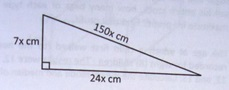
\includegraphics[width=5cm]{./img/quad1.jpg}
	\end{center}
	
	\begin{itemize}
	\item[(i)] Find the value of x
	\item[(ii)] Calculate the area of the triangle
	\end{itemize}		
	
	\item Given the right angled triangle below whose sides are measured in centimeters determine:
		\begin{itemize}
		\item[(i)] The value of x
		\item[(ii)] The area of the triangle
		\end{itemize}
		
		\begin{center}
		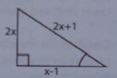
\includegraphics[width=3cm]{./img/quad2.jpg}
		\end{center}
		
	\item Study the following diagram carefully and answer the questions that follow.
	\begin{center}
	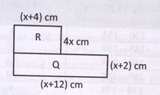
\includegraphics[width=4cm]{./img/quad3.jpg}
	\end{center}	
	
		\begin{itemize}
		\item[(a)]
			\begin{itemize}
			\item[(i)] Write down an expression for the area of rectangle R.
			\item[(ii)] Show that the total area of rectangle R and O is $(5x^2 + 30x + 24)$ cm$^2$.
			\end{itemize}					
		\item[(b)] If the total area of R and Q is 64 cm$^2$, calculate the value of $x$ correct to 1 decimal place.			
		\end{itemize}			

\end{enumerate}
	
	
	
	\subsection{Logarithms}
\begin{enumerate}

	\item Solve $\log_a(x^2 + 3) - \log_ax = 2\log_a2$.
	
	\item Evaluate without using mathematical tables $2\log 5 + \log 36 - \log 9$	
	
	\item Simplify $\cfrac{\log x^4 - \log x}{\log x^3 - \log x}$

	\item Simplify $2\log_{10} 25 - 3\log_{10} 5 + \log_{10} 20$.
	
	\item If $\log_a x = 7$, what is $\log_a \left(\cfrac{1}{x}\right)$?
	
	\item Find the value of the expression $2\log 40 + \log \sqrt{81} - 2\log 12$.
	
	\item Solve for $m$: $\log m = 3\log 6 - \frac{1}{3}\log 125 - 4\log 3 - \log \frac{16}{3}$

	\item Express as a single logarithm the expression $\frac{1}{2}\log_c x - 7\log_c y + \log_c z$.
	
	\item Without using tables, find the value of $3\log_{10} 5 + 5\log_{10} 2 - \frac{1}{2}\log_{10} 16$.
	
	\item Evaluate: $\log_3 9 \times \log_4 \cfrac{1}{64} \times \log_7 \cfrac{1}{7}$
	
	\item Simplify $\log_2 32 - \log_3 9$.
	
	\item It is given that $\log_{10} x + \log_{10} 20 = 2$. Find the value of $x$.
	
	\item Solve the equation $\log_4 5x - \log_4 (x + 2) - \log_4 3 = 0$.
	
	\item Evaluate without using tables $\log_5 \sqrt[3]{605}$
	
	\item If $\cfrac{\log k}{\log 9} = \cfrac{\log 256}{\log 16}$, find the value of $k$.
	
	\item Solve for $x$ in the logarithmic equation $2\log x = \log 4 + \log (2x - 3)$
	
	\item It is given that $n\log_5 125 = \log_2 64$. What is $n$?
	
	\item Find $x$ if $\log_x 32 = 5$.
	
	\item Solve for $x$ if $\log_{10} (x^2 - 3x - 44) = 1$
	
	\item If $\log_4 x = y$, show that $\log_2 x = 2y$. Hence find the value of $x$ given that $\log_2 x + \log_4 x = 9$.
	
	\item Find the value of $a$ if $\log_a 81 - \log_2 32 = -1$.
	
	\item Solve for $x$, given that $\log_3 x - \log_3 (x - 8) = 2$.
	
	\item Without using tables, calculate the value of\\
	(a) $\log_{10}6$	(b) $\log_{10}0.9$\\
	($\log_{10}2 = 0.3010$, $\log_{10}3 = 0.4771$)
	
	\item If $\log 2 = 0.3010$, find the value of $\log 5$.
	
	\item If $\log p = 1.813$ and $\log q = 2.513$, find the value of $pq^2$
	
	\item Using properties of logarithms show that $\log_{10} 15 = 1.17609$ given that $\log_{10} 2 = 0.30103$ and $\log_{10} 3 = 0.47712$.
	
	\item If $\log a = 1.3010$, $\log b = 1.4771$ and $\log c = 1.7782$, calculate $\log \sqrt{\cfrac{a^2b}{c^2}}$ 
	
	\item Evaluate $\log_{10} \cfrac{(0.1575 \times 27500)}{315}$ given that $\log_{10} 1.575 = 0.1973$, $\log_{10} 2.75 = 0.4393$ and $\log_{10} 3.15 = 0.4983$.

	\item Use logarithms to calculate $(3.25)^{10} + \left(\cfrac{40.9}{6.692}\right)^3$\\
	Express your answer in the form $A \times 10^n$, where $1 \leq A < 10$ and $n$ is an integer, to 2 significant figures.
	
	\item By using logarithm tables evaluate: $\sqrt{\cfrac{86.21 \times 2.734}{5.218 \times 0.724}}$
	
	\item Use common logarithm tables to find the value of $\cfrac{2.055 \times 20.35 \times 6.325}{100.5 \times 0.045}$
	
	\item By using logarithm tables evaluate: $\cfrac{88.76 \times 0.0278}{5678 \times 875.8}$

\end{enumerate}


	\subsection{Similarity / Congruence}
\begin{enumerate}

	\item In the figure drawn below find the value of $x$ if $\hat{B} = 37^\circ$.
	
	\begin{center}
	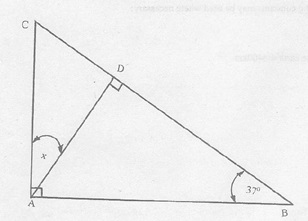
\includegraphics[width=5cm]{./img/sim1.jpg}
	\end{center}
	
	\item In the figure below DE is parallel to BC, AD = 6 cm, BD = 3 cm, DE = 4 cm and $A\hat{B}C = 90^\circ$.
	
	\begin{center}
	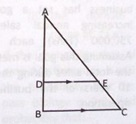
\includegraphics[width=3cm]{./img/sim2.jpg}
	\end{center}
	
	Calculate:
	\begin{itemize}
	\item[(i)] the length of BC
	\item[(ii)] the ratio AE\slash AC
	\end{itemize}
	
	\item In $\bigtriangleup ABC$, $M$ is the midpoint of $\overline{AB}$ and $N$ is the midpoint of $\overline{AC}$. Prove that $\overline{MN} \parallel \overline{BC}$ and $\overline{MN} = \frac{1}{2}\overline{BC}$.
	
	\item The ratio of the area of two similar triangles is 1 : 4. Find the ratio of their corresponding sides.
	
	\item If polygons $X$ and $Y$ are similar and their areas are 16 cm$^2$ and 49 cm$^2$ respectively, what is the length of a side of polygon $Y$ if the corresponding side of polygon $X$ is 28 cm?
	
	\item Triangles O and P are similar. A side of triangle O is 8 cm long, while the corresponding side of triangle P is 16 cm long. If the area of triangle O is 40 cm$^2$, what is the area of triangle P?
	
	\item 
		\begin{itemize}
		\item[(i)] Show whether triangles PQR and ABC are similar or not.
	\begin{center}
	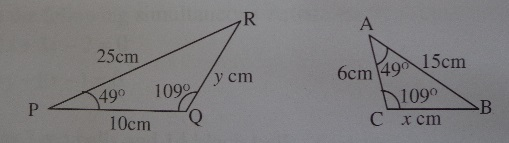
\includegraphics[width=7cm]{./img/sim14.jpg}
	\end{center}
		\item[(ii)] Find the relationship between $y$ and $x$ in the triangles given above.
		\end{itemize}
		
	\item In the figure below, SR is parallel to PQ, SX = 3 cm, XQ = 8 cm, PQ = 12 cm and XR = 2.7 cm.
	\begin{center}
	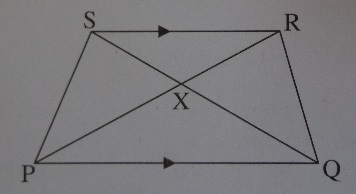
\includegraphics[width=4cm]{./img/sim15.jpg}
	\end{center}
		\begin{itemize}
		\item[(i)] Show that $\bigtriangleup PQX$ and $\bigtriangleup RSX$ are similar.
		\item[(ii)] Calculate the length of SR and PX.
		\end{itemize}
	
	\item With reference to the figure below, calculate the length of segment $\overline{CE}$.
	
	\begin{center}
	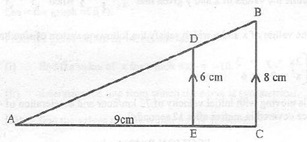
\includegraphics[width=5cm]{./img/sim3.jpg}
	\end{center}

		\item In the figure below, calculate the length $\overline{BC}$ if $\overline{AD} = 4$ cm, $\overline{DE} = 3$ cm, $\overline{CE} = 5$ cm and $A\hat{B}C$ and $A\hat{D}E$ are both right angles.
	
	\begin{center}
	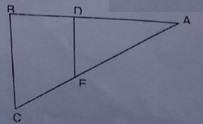
\includegraphics[width=4cm]{./img/sim10.jpg}
	\end{center}

	\item In the figure below, BC is parallel to DE, AB = AC and CE = 2.5 cm. DE = 6 cm. The height of trapezium BCED is 1.5 cm.
	
	\begin{center}
	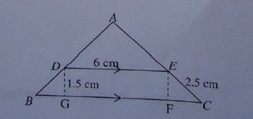
\includegraphics[width=5cm]{./img/sim4.jpg}
	\end{center}

	\begin{itemize}
	\item[(a)] Prove that the triangles ABC and ADE are similar.
	\item[(b)] Calculate the length of AE.
	\end{itemize}
	
	\item In the diagram below, show that $\cfrac{AD}{AB} = \cfrac{CD}{AC}$
	
	\begin{center}
	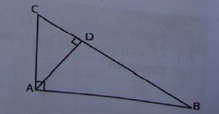
\includegraphics[width=5cm]{./img/sim7.jpg}
	\end{center}

	\item $\bigtriangleup ABC$ is similar to $\bigtriangleup DEF$. AB = 8 cm while DE = 12 cm. Find the area of $\bigtriangleup ABC$ if that of $\bigtriangleup DEF$ is 45 cm$^2$.
	
	\item In the figure below, $\overline{PQ} \parallel \overline{BC}$, $\overline{AP} = 3$ cm, $\overline{AQ} = 2$ cm and the area of $\bigtriangleup APQ = 8$ cm$^2$.
	\begin{center}
	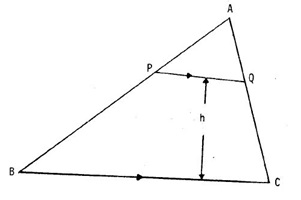
\includegraphics[width=5cm]{./img/sim8.jpg}
	\end{center}

	\begin{itemize}
	\item[(a)] Show that $\bigtriangleup APQ$ is similar to $\bigtriangleup ABC$
	\item[(b)] Find the area of $\bigtriangleup ABC$
	\item[(c)] Calculate the length of (i) $\overline{PQ}$  \quad (ii) $\overline{QC}$ 
	\item[(d)] Calculate the height $h$.
	\end{itemize}
	
	\item In the figure below, $m(A\hat{B}C) = 90^\circ$. Point D on $\overline{BC}$ is such that $\overline{AD}$ bisects $B\hat{A}C$. If AD = 4 cm and $m(A\hat{D}B) = 60^\circ$, calculate the length of:
		\begin{itemize}
		\item[(a)] $\overline{AB}$
		\item[(b)] $\overline{DC}$
		\end{itemize}
		
	\begin{center}
	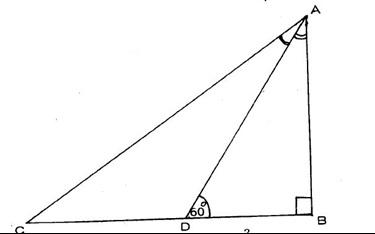
\includegraphics[width=6cm]{./img/sim9.jpg}
	\end{center}
	
	\item In the figure below, $\bigtriangleup ABC$ is similar to $\bigtriangleup CTU$, with AB = 3 cm and CT = 2 cm. The area of $\bigtriangleup CTU$ is 6 square cm. Find the area of $\bigtriangleup ABC$.
	
	\begin{center}
	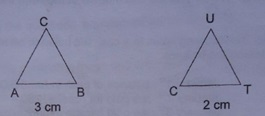
\includegraphics[width=5cm]{./img/sim11.jpg}
	\end{center}
	
	\item PXQ and RXS are straight lines and PR is parallel to SQ. Calculate PX and RX if PR = XQ = 18 cm, XS = 9 cm and SQ = 12 cm.
	
	\begin{center}
	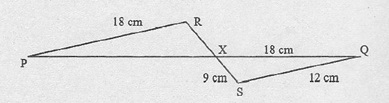
\includegraphics[width=7cm]{./img/sim12.jpg}
	\end{center}	
	
	\item In the figure below, ABCD is a square. If $\overline{AR} = \overline{BR}$ prove that R is the midpoint of $\overline{DC}$.
	
	\begin{center}
	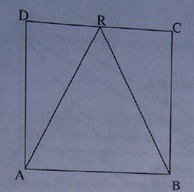
\includegraphics[width=3cm]{./img/sim13.jpg}
	\end{center}	
	
	
%congruency	
	\item ABCD is part of a regular polygon. Show that the triangles ABC and BCD are congruent.
	
	\begin{center}
	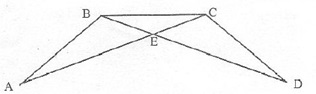
\includegraphics[width=5cm]{./img/sim5.jpg}
	\end{center}
	
	\item In the figure below, $\overline{AC} = \overline{CB}$ and $D\hat{A}C$ and $D\hat{B}C$ are right angles. Prove that $\bigtriangleup ACD \equiv \bigtriangleup CBD$.
	
	\begin{center}
	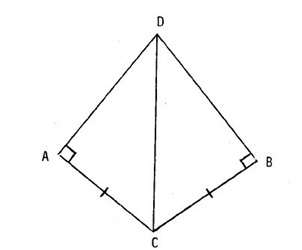
\includegraphics[width=5cm]{./img/sim6.jpg}
	\end{center}
	
\end{enumerate}	

	\subsection{Geometrical Transformations}
	
	See Form IV \nameref{f4trans}.

	\subsection{Pythagoras Theorem}
	
	See \nameref{f2quadeqnsgeo} in Form II \nameref{f2quadeqns} as well as applications in Form IV \nameref{f4trig}.
	
	\subsection{Trigonometry}
	
	See Form IV \nameref{f4trig}.
	
	\subsection{Sets}
\begin{enumerate}

	\item A survey conducted at Omega secondary school showed that 15 students play volleyball, 11 play basketball and 6 play both volleyball and basketball. If everyone plays at least one of these games, find the number of students who play the following games (using a Venn diagram):
		\begin{itemize}
		\item[(a)] volleyball or basketball;
		\item[(b)] basketball but not volleyball;
		\item[(c)] volleyball only.
		\end{itemize}

	\item In a class of 30 students, 17 participate in English debate, 12 participate in English debate and sports. If every student is required to participate in at least one of these two events, find the number of students who participate in:
	\begin{itemize}
	\item[(i)] English debate only
	\item[(ii)] sports only.
	\end{itemize}

	\item In a class of 42 students, 31 students study History and 26 study Physics. Using VVenn diagrams or otherwise, find the number of students who study Physics only.
	
	\item In a certain school there are 50 pupils studying both Basic Mathematics and Additional Mathematics. School regulations require that an Additional Mathematics pupil must come from the Basic Mathematics class. In the school, 10 pupils do not study Basic Mathematics. If only 100 pupils study Basic Mathematics but not Additional Mathematics, how many pupils:
	\begin{itemize}
	\item[(i)] are in the school?
	\item[(ii)] study either Basic Mathematics or Additional Mathematics?
	\item[(iii)] do not study Additional Mathematics?
	\end{itemize}
	\noindent Hint: (Use Venn diagram)
	
	\item There are 60 people at a meeting. 35 are businesspersons, 32 are employees and 15 are both businesspersons and employees.
	\begin{itemize}
	\item[(i)] How many are businesspersons or employees?
	\item[(ii)] How many are neither businesspersons nor employees?
	\end{itemize}
	
	\item There are 30 men at a wedding. Twenty are businessmen, twelve are fishermen and 6 are both businessmen and fishermen.
	\begin{itemize}
	\item[(i)] How many are neither businessmen nor fishermen?
	\item[(ii)] How many are either businessmen or fishermen?
	\end{itemize}
	
	\item 
	\begin{itemize}
	\item[(a)] In a boys' school of 200 students, 90 play football, 70 play basketball and 50 play tennis; 26 play basketball and football, 20 play basketball and tennis, 16 play tennis and football while 10 play all three games. Represent this information in a well labeled Venn diagram.
	\item[(b)] From the information given in (a), how many students in the school do not play:
	\begin{itemize}
	\item[(i)] football
	\item[(ii)] basketball
	\item[(iii)] tennis.
	\end{itemize}
	\end{itemize}
	
	\item Student test results on three subjects; Mathematics, Physics and Chemistry show that 20 passed Chemistry, 5 passed all three subjects, 12 passed Mathematics and Physics and 16 passed Mathematics and Chemistry. Each student passed at least two subjects.
	\begin{itemize}
	\item[(i)] Draw a well labeled Venn diagram to represent these results.
	\item[(ii)] How many students passed Physics and Chemistry?
	\item[(iii)] How many students did the test?
	\end{itemize}

	\item A survey of 240 houses showed that all of them kept a farm or a garden or both. If 180 kept gardens and 79 kept farms, how many houses kept both?
	
	\item In a school of 75 pupils, 45\% of the pupils take Biology but not Chemistry, 32\% take both subjects and 10\% of them take Chemistry but not Biology. How many pupils do not take either Biology or Chemistry?
	
	\item In a Form four class of 24 students, 10 students take basic mathematics only, 12 students take physics and 4 students take both subjects. Using a Venn diagram, find:
	\begin{itemize}
	\item[(i)] The number of students taking physics only.
	\item[(ii)] The number of students taking mathematics.
	\item[(iii)] The number of students who take neither of the two subjects
	\end{itemize}
	
	\item In a class of 36 students, 24 take Chemistry whilst 17 take Physics. What is the least possible number of students who must be taking both Physics and Chemistry?
	
	
%not word problems	
	\item $A$ and $B$ are subsets of the universal set $U$. Find n$(A \cap B)$ given that n$(A) = 39$, n$(A' \cap B') = 4$, n$(B') = 24$ and n$(U) = 65$.

	\item Given $A = \{(x,y):3x + 4y = 10\}$ and $B = \{(x,y):2x - 3y = 1\}$, find $A \cap B$.
	
	\item If $\mu = \{x:1 < x < 11\}$, $A = \{x:2 < x \leq 9\}$, $B = \{x:2 \leq x < 10\}$, list the elements belonging to:
	\begin{itemize}
	\item[(i)] $A \cup B$
	\item[(ii)] $A' \cap B$
	\end{itemize}
	
	\item $P$ and $Q$ are finite sets such that n$(P \cap Q') = 15$, n$(P \cup Q) = 90$ and n$(P \cap Q) = 30$. Without using a Venn diagram, find n$(Q)$.
	
	\item If $A = \{a, b, c\}$, $B = \{b, c, d\}$ and $C = \{c, d, e\}$, show that $A \cup (B \cap C) = (A \cup B) \cap (A \cup C)$.
	
	\item If $\xi = \{a, b, c, d, e\}$, $A = \{a, b, c\}$ and $B = \{e, d\}$, find:
		\begin{itemize}
		\item[(i)] $A' \cap B'$
		\item[(ii)] $(A \cap B)'$
		\end{itemize}
		
	\item If n$(A) = 8$, n$(B) = 12$ and $(A \cap B) = 5$, find n$(A \cup B)$.
		
	\item If $\mu = \{p, q, r, s\}$, If $A = \{p, q, r\}$ and If $B = \{r, s\}$, find $(A' \cap B')$.
		
	\item If $A$ and $B$ are subsets of $S$ where\\
	$S = \{x: x$ is a natural number less than 20$\}$\\
	$A = \{x: x$ is an even number$\}$\\
	$B = \{x: x$ is a multiple of 3$\}$\\
	Find: (a) n$(A \cap B)$ \quad (b) n$(A' \cup B')$
	
	\item If $A$ is the set of prime factors of 42 and $B$ is the set of prime factors of 330, find n$(A \cap B)$.
	
	\item Given sets $A = \{x:-5 \leq x < 2\}$ and $B = \{x:-1 < x < 4\}$, find the value of $A \cap B$.
	
	\item Given $N = \{x:1 \leq x \leq 20\}$. Find the following subsets of $N$:
		\begin{itemize}
		\item[(i)] $A = \{x: x$ is a multiple of 3$\}$
		\item[(ii)] $B = \{x: x$ is a multiple of 4$\}$
		\item[(iii)] $A'$ \quad (iv) $B'$ \quad (v) $(A \cup B)'$ \quad and \quad (vi) $A' \cap B'$.
		\end{itemize}
		
	\item If $A$ and $B$ are any two disjoint sets, show the region represented by $A' \cap B'$ on a Venn diagram.
	
	\item $U = \{10, 20, 30, 40\}$, $A = \{10, 30\}$, $B = \{40, 10\}$, find:
		\begin{itemize}
		\item[(a)]
			\begin{itemize}
			\item[(i)] $A' \cup B'$
			\item[(ii)] $A \cap B'$
			\end{itemize}
		\item[(b)] If $A$ is a subset of $B$, represent the two sets in a Venn diagram.
		\end{itemize}
		
	\item If n$(A \cap B') = 8$, n$(B \cap A') = 5$ and n$(A \cup B) = 20$, 
		\begin{itemize}
		\item[(i)] Display the information in a Venn diagram.
		\item[(ii)] Give the values of n$(A)$ and n$(B)$.
		\end{itemize}
		
	\item Given that $A = \{x:0 \leq x \leq 8\}$ and $B = \{x:3 \leq x \leq 11\}$, where $x$ is an integer, in the same form, present in a Venn diagram:\\
	(i) $A \cup B$ \quad (ii) $A \cap B$\\
	and hence find the elements in each set.
	
	\item If $E = \{$integers between 1 and 11$\}$\\
	$A = \{x:2 < x \leq 9\}$\\
	$B = \{x:1 \leq x < 10\}$
		\begin{itemize}
		\item[(a)] Draw a Venn diagram to illustrate these sets.
		\item[(b)] List the elements belonging to:\\
			(i) $A \cup B$ \quad (ii) $A' \cap B$
		\item[(c)] State n$(A \cap B')$
		\end{itemize}
		
	\item From the figure below, answer the following questions.
	
	\begin{center}
	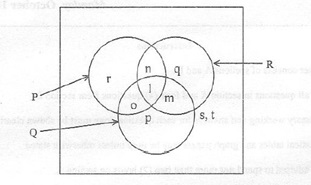
\includegraphics[width=6cm]{./img/set1.jpg}
	\end{center}
	
	\begin{itemize}
	\item[(a)] List down members of $(P \cup Q)'$
	\item[(b)] Find n$(P \cup Q \cup R)'$
	\item[(c)] Find n$(Q \cup R) - $ n$(P \cap R)$
	\end{itemize}
	
	\item In the Venn diagram below, the number of elements in various regions are as indicated.\\
	If n$(A \cup B \cup C) = 150$, find the value of $x$.
	
	\begin{center}
	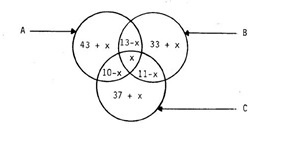
\includegraphics[width=7cm]{./img/set2.jpg}
	\end{center}
	
	\item In the figure drawn below, find the number of elements in sets:
		\begin{itemize}
		\item[(a)] $A' \cap (B \cup C)$
		\item[(b)] $(A' \cap B') \cup (B \cup C')$
		\end{itemize}
		
	\begin{center}
	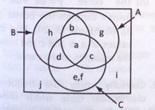
\includegraphics[width=5cm]{./img/set3.jpg}
	\end{center}
	

\end{enumerate}


	\subsection{Statistics}
	
	See Form III \nameref{f3stats}.


\section{Form III}

	\subsection{Relations / Functions}
\begin{enumerate}


			\subsubsection{Graphs, Domain, Range}
%relations

	\item Consider the relation $R = \{(x,y): y = x^2 + 4x\}$
		\begin{itemize}
		\item[(a)] Complete the following table for the relation $R$.\\
		\begin{tabular}{|c|c|c|c|c|c|c|c|c|c|c|} \hline
		$x$ &-6&-5&-4&-3&-2&-1&0&1&2&3 \\ \hline
		$y$ &&&&&&&&&& \\ \hline
		\end{tabular}
		\item[(b)] Plot the graph of the relation $R$.
		\item[(c)] Use the graph to solve the equation $x^2 + 3 = -4x$.
		\end{itemize}
		
	

		
%functions
	\item A function $f$ is defined by $f: \rightarrow 2x^2 - 2x - 1$ where $x$ is the set $\{-2, -1, 0, 1, 2, 3\}$;
		\begin{itemize}
		\item[(a)] Write down the set of ordered pairs $(x, f(x))$.
		\item[(b)] Represent the set of ordered pairs $(x, f(x))$ in a pictorial diagram.
		\item[(c)] Draw the graph of $f(x)$.
		\item[(d)] Find the maximum or minimum value of the function $f(x) = 2x^2 - 2x - 1$.
		\end{itemize}

	\item A function $f$ is defined by the formula $f(x) = \sqrt{x}$, where $x$ is a whole number.
		\begin{itemize}
		\item[(a)] Evaluate $f(9)$
		\item[(b)] If $f(x) = 16$, find the value of $x$.
		\item[(c)] Find the value of $\cfrac{f(200)}{f(2)}$
		\end{itemize}		
		
	\item A function $f$ is defined by: $f(x) = |x - 2|$.
		\begin{itemize}
		\item[(i)] Evaluate $f(-3)$.
		\item[(ii)] Find $x$ if $f(x) = 6$.
		\end{itemize}		 
		
	\item If $f(x) = 5x^2 + 17x - 12$,
		\begin{itemize}
		\item[(a)]
			\begin{itemize}
			\item[(i)] Evaluate $f(10) - f(5)$
			\item[(ii)] Factorize $f(x)$
			\end{itemize}
		\item[(b)] Determine the domain and range of $f(x)$
		\end{itemize}
		
	\item The curve $y = ax^2 + bx + c$ passes through the points (1,8), (0,5) and (3,20). Find the values of $a$, $b$ and $c$ and hence the equation of the curve.
	
	\item If $f(x) = \cfrac{x + 2}{x^2 - x- 6}$, find the values of $x$ for which the function is not defined.
	
	\item The function $f$ is defined by $f: \rightarrow ax + b$, for $x \in R$, where $a$ and $b$ are constants. It is given that $f(2) = 1$ and $f(5) = 7$.
		\begin{itemize}
		\item[(i)] Find the value of $a$ and $b$
		\item[(ii)] Solve the equation $f \circ f(x) = 0$
		\end{itemize}
		
	\item Draw the graph of $x^2 = 2 + y$.
	
	\item It has been specified that $f(x) = 2x^2 - 5x - 3$ ranges from $x = -2$ to $x = 4$.
		\begin{itemize}
		\item[(a)] Draw the graph of $f(x)$.
		\item[(b)] From the graph drawn in (a) above:
			\begin{itemize}
			\item[(i)] find the value of $x$ for which $f(x) = -10$.
			\item[(ii)] determine the line from which the curve is symmetrical.
			\item[(iii)] find the values of $x$ by which $f(x)$ is negative.
			\item[(iv)] solve the equation $2x^2 - 5x - 3 = 0$.
			\end{itemize}
		\end{itemize}

	\item A function is defined by $f(x) = \cfrac{x}{x + 3}$; sketch the graph of $f$.
	
	\item 
		\begin{itemize}
		\item[(a)] On the same set of axes draw the graphs of $f(x) = x^2 - 4x$ and $y = x - 2$.
		\item[(b)] Using the two graphs in (a), estimate the values of $x$ for which $x^2 - 5x + 2 = 0$, correct to 2 significant digits.
		\end{itemize}
		
		\item Without using a table of values, draw the graph of $y = -x^2 + 4x - 5$ and use it to solve the equation $-x^2 + 4x - 5 = -10$.
		
		\item Sketch the graph of the function $f(x) = -1 + |x|$ and find:
			\begin{itemize}
			\item[(i)] the domain and \quad (ii) the range, of $f(x)$.
			\end{itemize}
			
	\item Sketch the graph of the rational function $y = \cfrac{3x - 4}{x - 3}$ and determine its range.
	
	\item 
		\begin{itemize}
		\item[(a)] 
			\begin{itemize}
			\item[(i)] Draw the graphs of the functions $f(x) = x^2 - 4$ and $g(x) = x + 2$ in the same coordinate system.
			\item[(ii)] Shade the region enclosed by the graphs in (i) indicating the intercepts for both graphs.
			\end{itemize}
		\item[(b)] From the graphs in (a) write the coordinates of the points where $f(x) = g(x)$.
		\item[(c)] State the domain and range of $f(x)$.
		\end{itemize}
		
	\item The functions $f$ and $g$ are defined for the domain: $\{2, 3, 4, 5, 6\}$ and the range of $f = \{8, 10, 12, 14, 16\}$ and that of $g = \{8, 6, 4, 2, 0\}$. Find $fg(3)$.
	
	\item Find the domain and range of $f(x) = \sqrt{1 - x^2}$.
	
	\item Find the domain and range of the relation $y = 3x^2 + 2$.
	
	\item Compute the range of the function $f(x) = x^2 - 4x + 3$ for which the domain is $\{-2, -1, 0, 1, 2, 3\}$.
	
	\item Given the rational function $g(x) = \cfrac{mx^2}{x^2 - 3x + 2}$, determine its domain and range.
	
	\item If $f$ is a function such that:\\
	$f(x) =
	\begin{cases}
	\-3 & \text{if } x \leq -1 \\
	1 & \text{if } -1 < x \leq 2 \\
	4 & \text{if } 2 < x
	\end{cases}$
	
	\begin{itemize}
	\item[(a)] determine the domain and range of $f(x)$.
	\item[(b)] draw the graph of $f(x)$.
	\end{itemize}
	
			\subsubsection{Inverse Functions}
%inverses	
	\item Write down the inverse of the function $f(x) = \frac{1}{2}x + 5$.
	
	\item If $f(x) = \frac{1}{2}x + 5$, find $f^{-1}(6)$.
	
	\item A function is defined by $f(x) = x^2 - 2$. Find:
		\begin{itemize}
		\item[(i)] the inverse, $f^{-1}(x)$ of this function.
		\item[(b)] the value of $f^{-1}(-2)$.
		\item[(c)] the domain of $f^{-1}(x)$.
		\end{itemize}
		
	\item Find $g^{-1}(x)$ and hence evaluate $g^{-1}(18)$ given that $g(x) = 2^x + 2$.
	
	\item Find the inverse of the relation $y = \cfrac{4x + 1}{x - 2}$.
	
	\item Find the inverses of the following:
		\begin{itemize}
		\item[(a)] $\{R = (x,y): y = 4x^2\}$
		\item[(b)] $f(x) = 20^x$
		\end{itemize}
		
	\item The functions $f$ and $g$ are defined by: $f(x) = |x|$ and $g(x) = 2 - 3x$.
		\begin{itemize}
		\item[(i)] Evaluate $f(-3)$.
		\item[(ii)] Find $g^{-1}(x)$ and hence evaluate $g^{-1}(8)$.
		\item[(iii)] Draw on the same axes the graphs of $f$ and $g$.
		\end{itemize}

	\item 
		\begin{itemize}
		\item[(a)] If $f(x) = -2x + 3$ find $f^{-1}(3)$.
		\item[(b)] Draw the graph of $f(x) = |x - 1|$ for $-4 \leq x \leq 4$
		\item[(c)] State the domain and range of $f(x) = |x - 1|$.
		\end{itemize}
		
	\item If $f(x) = x^2 - 4x + 3$, find\\
	(i) $f^{-1}(x)$ \quad (ii) the domain and range of $f(x)$
	
	\item A function is defined by $f(x) = x^2 + 6$ and $g(x)$ is another function of $x$ such that\\
	 $g(x) = \cfrac{f(x) - f(4)}{x - 4}$. \\
	Find (i) $g(-4)$ \quad (ii) $g^{-1}(5)$
	
	\item Given that $g(x) = 5 + \cfrac{x}{2}$, find the values of:\\
	(i) $g^{-1}(6)$ \quad (iii) $g^{-1}(-1)$\\
	(ii) $g^{-1}(0)$ \quad (iv) $g^{-1}(a)$
	
			\subsubsection{Maximum, Minimum Values}
%max, min value	
	\item Find the maximum value of the quadratic equation $2 + 30t - 5t^2$.
	
	\item Draw a graph of the function $y = x^2 - 3x + 2$ for the values of $x$ from -2 to 5. From your graph, find:
		\begin{itemize}
		\item[(a)] the range of the function.
		\item[(b)] the minimum value of $y$ and the value of $x$ at which this minimum value occurs.
		\item[(c)] the solution of the equation $x^2 - 3x - 4 = 0$.
		\item[(d)] the solution of the inequality $x^2 - 3x + 2 > 0$.
		\end{itemize}
		


\end{enumerate}	
	
	
	
	
	\subsection{Statistics} \label{f3stats}
\begin{enumerate}

	\item The table below show the distribution of the ages of boys in one class at Shivone secondary school.\\
	\begin{tabular}{|l|c|c|c|c|} \hline
	Age in years & 14 - 16&17 - 19&20 - 22&23 - 25\\ \hline
	Number of boys&27&14&8&7\\ \hline	
	\end{tabular}
		\begin{itemize}
		\item[(a)] Draw a cumulative frequency polygon for this information.
		\item[(b)] What is the mean age of the class?
		\item[(c)] State the median class.
		\item[(d)] Find the probability that a boy chosen at random from the class has age between 17 - 19 or 23 - 25.
		\end{itemize}

	\item In a survey of the number of children in 12 houses, the following data resulted: 1, 2, 3, 4, 2, 2, 1, 3, 4, 3, 5, 3.
		\begin{itemize}
		\item[(a)] Show this data in a frequency distribution table.
		\item[(b)] Draw a histogram and a frequency polygon to represent this data.
		\item[(c)] Calculate the mean and mode number of children per house.
		\end{itemize}

	\item The following is a record of marks by a group of students in an examination.\\
	
	\begin{tabular}{cccccccccc}
	23&63&82&71&12&63&38&17&23&44 \\
	54&19&70&45&70&43&18&03&02&64 \\
	45&42&40&70&63&28&18&27&58&53 \\
	23&81&70&58&31&83&19&43&72&71 \\
	48&63&62&44&38&37&46&81&73&38 	
	\end{tabular}
	
	\begin{itemize}
	\item[(a)] Tabulate as a frequency distribution using intervals 0 - 9, 10 - 19, etc.
	\item[(b)] Find the class which contains the median.
	\item[(c)] Find the modal class.
	\item[(d)] Calculate the mean mark using the grouped data.
	\end{itemize}
	
	\item The following frequency distribution table shows the monthly salaries for 33 workers in a certain company.\\
	
	\begin{tabular}{|p{2.5cm}|c|c|c|c|c|} \hline
	\textbf{Salary (Tsh)}&20000 - 29000&30000 - 39000&40000 - 49000&50000 - 59000&60000 - 69000 \\ \hline
	\textbf{Number of Workers}&1&4&6&10&8 \\\hline
	\end{tabular}

	\begin{tabular}{|p{2.5cm}|c|c|} \hline
	\textbf{Salary (Tsh)}&70000 - 79000&80000 - 89000 \\ \hline
	\textbf{Number of Workers}&2&2 \\\hline
	\end{tabular}
	
	\begin{itemize}
	\item[(a)] By making the class mark of the class interval 50000 - 59000 as the assumed mean, calculate the mean salary.
	\item[(b)] What is the mode for this distribution?
	\item[(c)] Calculate the median.
	\item[(d)] Find the number of workers whose salaries exceed Tsh 69,500/=.
	\end{itemize}
	
	\item The following table gives the scores of sixty students in a Basic Mathematics test.\\
	
	\begin{tabular}{|c|c|} \hline
	Scores&Frequency \\ \hline
	0 - 10&5 \\ \hline
	10 - 20&7 \\ \hline
	20 - 30&15 \\ \hline
	30 - 40&25 \\ \hline
	40 - 50&8 \\ \hline
	\end{tabular}
	
	Calculate:
	\begin{itemize}
	\item[(a)] The mean score if the assumed mean is obtained from the mid mark of the modal class.
	\item[(b)] The median.
	\item[(c)] The range.
	\end{itemize}
	
	\item Carefully study the frequency distribution table which shows marks for 40 students in a mathematics examination.\\
	
	\begin{tabular}{|l|c|c|c|c|c|} \hline
	Marks & 1 - 20&21 - 40&41 - 60&61 - 80&81 - 100\\ \hline
	Number of Students&3&11&12&8&6\\ \hline	
	\end{tabular}
	
	\begin{itemize}
	\item[(i)] Calculate the mean score, given the assumed mean 50.5.
	\item[(ii)] Determine the modal class.
	\item[(iii)] Draw a cumulative frequency curve and use it to estimate the median.
	\end{itemize}
	
	\item A survey of 50 families showed the number of children per family as follows.\\
	
	\begin{tabular}{|l|c|c|c|c|c|} \hline
	Number of children&1&2&3&4&5 \\ \hline
	Number of families&19&18&9&3&1 \\ \hline	
	\end{tabular}
	
	\begin{itemize}
	\item[(i)] Write down the modal number of children per family.
	\item[(ii)] Find the median number of children per family.
	\item[(iii)] Calculate the mean number of children per family.
	\end{itemize}
	
	\item The age at which a child first walked (to the nearest month) was recorded for eight (8) children. The results were 12, 10, 16, 19, 10, 12, 12 and 13. Calculate the mean, mode and median of the data.
	
	\item A random sample of 100 students was chosen from a school. Each student's blood pressure was measured to the nearest milimetres of mercury as shown in the table below.\\
	
	\begin{tabular}{|l|c|c|c|c|c|c|c|} \hline
	Blood pressure (mmHg)&55 - 59&60 - 64&65 - 69&70 - 74&75 - 79&80 - 84&85 - 89 \\ \hline
	Number of students&1&3&8&17&30&25&16 \\ \hline
	\end{tabular}
	
	\begin{itemize}
	\item[(a)] Calculate the mean and mode of blood pressure.
	\item[(b)] Construct a cumulative frequency table and draw the ogive. From the ogive estimate
		\begin{itemize}
		\item[(i)] the median blood pressure
		\item[(ii)] the percentage of students with blood pressure between 67 mmHg and 76 mmHg.
		\end{itemize}
	\end{itemize}
	
	\item Carefully study the frequency distribution table for the scores of 68 students (in percentage) given here under.\\
	
	\begin{tabular}{|p{3cm}|c|c|c|c|c|c|c|} \hline
	Class Boundary (in percentage)&30 - 39&40 - 49&50 - 59&60 - 69&70 - 79&80 - 89&90 - 99 \\ \hline	
	Frequency&6&12&14&16&8&6&6 \\ \hline
	\end{tabular}
	
	\begin{itemize}
	\item[(a)] Determine the mode of the scores.
	\item[(b)] Calculate the median of the scores.
	\item[(c)] A student is chosen at random from the frequency distribution table above. What is the probability that his score is below 60\%?
	\end{itemize}
	
	\item A survey was made on the number of the people attending conferences on one particular week. A random sample of 100 conference centres was taken and the results were as follows:\\
	
	\begin{tabular}{|c|c|} \hline
	\textbf{Number of people}& \textbf{Number of}\\ 	\textbf{attending conference}&\textbf{conference centres} \\ \hline
	150 - 154&8 \\ \hline
	155 - 159&16 \\ \hline
	160 - 164&43 \\ \hline
	165 - 169&29 \\ \hline
	170 - 174&4 \\ \hline	
	\end{tabular}
	
	\begin{itemize}
	\item[(i)] Draw a histogram and a cumulative frequency curve to represent these results.
	\item[(ii)] Estimate the median of this data from the cumulative frequency curve in (i) above.
	\end{itemize}
	
	\item The pie chart below shows the number of students in one examination centre in different subjects sat for the national examinations.
	
	\begin{center}
	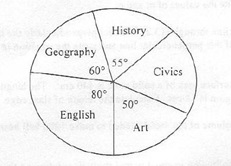
\includegraphics[width=5cm]{./img/stats1.jpg}
	\end{center}
%	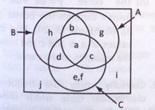
\includegraphics[width=5cm]{./img/set3.jpg}
%	\end{center}	
	
	Given that 220 candidates did History, find:
	\begin{itemize}
	\item[(i)] The total number of candidates at this examination centre.
	\item[(ii)] The number of students who sat for Civics examination.
	\end{itemize}
	
	\item The following represents age distribution of members of a school choir.\\
	
	\begin{tabular}{|l|c|c|c|c|c|c|} \hline
	Age&14&15&16&17&18&19 \\ \hline
	Frequency&2&1&3&6&5&3 \\ \hline	
	\end{tabular}
	
	\begin{itemize}
	\item[(a)] How many students are in the school class?
	\item[(b)] What is the modal age?
	\item[(c)] Calculate the mean age of the members of the school choir.
	\item[(d)] What is the probability that a member chosen at random from the choir is
		\begin{itemize}
		\item[(i)] 17 years old?
		\item[(ii)] over or equal to 17 years?
		\end{itemize}
	\item[(e)] Draw a pie chart to show the age distribution of the members of the school choir.
	\end{itemize}
	
	\item The data below represent masses in kg of 36 men:\\
	51; 61; 60; 70; 75; 71; 75; 70; 74; 73; 72; 82; 70; 71; 76; 74; 50; 68; 68; 66; 65; 72; 69; 64; 83; 63; 83; 58; 80; 90; 50; 89; 55; 62; 62; 61.
	\begin{itemize}
	\item[(i)] Prepare a frequency distribution table of class interval of size 5 beginning with the number 50 taking into consideration that both the lower limit and upper class limit are inclusive.
	\item[(ii)] Calculate the mean and mode from the frequency distribution table prepared in (i) above by using assumed mean from the class mark of the modal class.
	\end{itemize}
	
	\item The data below shows test scores of a certain class in mathematics.
	
	\begin{tabular}{cccccccccc}
	21&21&21&22&22&22&22&23&23&24 \\
	24&24&21&24&24&25&26&27&27&27 \\
	\end{tabular}
	
	Construct a frequency distribution table showing scores $x$ and frequency $f$.
	
	\item Carefully study the frequency distribution table which shows marks for 40 students in a mathematics examination.\\
	
	\begin{tabular}{|l|c|c|c|c|c|} \hline
	Marks & 1 - 20&21 - 40&41 - 60&61 - 80&81 - 100\\ \hline
	Number of Students&3&11&12&8&6\\ \hline	
	\end{tabular}
	Determine:
	\begin{itemize}
	\item[(i)] The mean, given the assumed mean is 50.5
	\item[(ii)] The median
	\item[(iii)] Modal class and its corresponding class mark.
	\end{itemize} 
	
	\item The table shows the masses of 100 students to the nearest kilogram.\\
	
	\begin{tabular}{|l|c|c|c|c|c|} \hline
	Mass (kg) &60 - 62&63 - 65&66 - 68&69 - 71&72 - 74 \\ \hline
	Frequency&5&18&42&27&8 \\ \hline	
	\end{tabular}
	
	\begin{itemize}
	\item[(a)] Determine the mean of the masses.
	\item[(b)] Find the mode.
	\item[(c)] Draw a cumulative frequency curve and use it to determine the median of the masses.
	\end{itemize}
	
	\item The table below shows the distribution of 100 shops and their profit per shop recorded in a certain month.\\
	
	\begin{tabular}{|l|c|c|c|c|c|c|} \hline
	Profit per shop in thousands of shs.&30 - 34&35 - 39&40 - 44&45 - 49&50 - 54&55 - 59 \\ \hline
	Number of shops&12&18&C&C - 7&C - 10&6 \\ \hline	
	\end{tabular}
	
	\begin{itemize}
	\item[(a)] Find the value of C.
	\item[(b)] Prepare the frequency distribution and use it to determine the modal class.
	\item[(c)] Draw a histogram and frequency polygon on the same diagram.
	\end{itemize}
	
	\item The frequency distribution of the length of a sample of 100 nails, measured to the nearest mm, is shown below.\\
	
	\begin{tabular}{|l|c|c|c|c|c|c|c|} \hline
	Length&40 - 42&43 - 45&46 - 48&49 - 51&52 - 54&55 - 57&58 - 60 \\ \hline
	Frequency&4&9&13&20&34&18&2 \\ \hline	
	\end{tabular}
	
	\begin{itemize}
	\item[(a)] How many nails have length less than 51.5 mm?
	\item[(b)] Calculate the mean length.
	\item[(c)] Draw a histogram and use it to estimate the modal length.
	\item[(d)] State the modal class.
	\end{itemize} 
	
	\item The daily wages of one hundred men are distributed as shown below:\\
	
	\begin{tabular}{|p{4cm}|c|c|c|c|} \hline
	Wage in Tshs $\times$ 1000&3.0 - 3.4&3.5 - 3.9&4.0 - 4.4&4.5 - 4.9 \\ \hline
	Number of men&4&6&10&14 \\ \hline	
	\end{tabular}
	
	\begin{tabular}{p{4cm}|c|c|c|c|} \cline{2-5}
	&5.0 - 5.4&5.5 - 5.9&6.0 - 6.4&6.5 - 6.9 \\ \cline{2-5}
	&x&20&14&6 \\ \cline{2-5}	
	\end{tabular}
	
	\begin{itemize}
	\item[(a)] Find x.
	\item[(b)] Calculate the daily mean wage of the 100 men.
	\item[(c)] Draw a histogram to represent this data.
	\end{itemize}
	
	\item The table below shows the distribution of scores of 46 students in a mathematics examination.\\
	
	\begin{tabular}{|l|c|c|c|c|c|} \hline
	Marks in \%&35 - 45&46 - 56&57 - 67&68 - 78&79 - 89 \\ \hline
	No. of students&20&12&7&6&1 \\ \hline	
	\end{tabular}
	
	\begin{itemize}
	\item[(a)] 
		\begin{itemize}
		\item[(i)] Calculate the mean score.
		\item[(ii)] What is the modal class?
		\end{itemize}		 
	\item[(b)] Draw a cumulative frequency curve and estimate from  it the median score.
	\end{itemize} 
	
	\item The heights in centimetres of 100 students of a certain school were recorded as follows:\\
	
	\begin{tabular}{|l|c|c|c|c|c|c|c|c|c|} \hline
	Height in cm&150&155&160&165&170&175&180&185&190 \\ \hline
	Frequency&4&9&12&16&25&20&8&4&2 \\ \hline	
	\end{tabular}
	
	From the above information answer the following questions:
	\begin{itemize}
	\item[(a)] Draw a frequency polygon.
	\item[(b)] Determine the mean, median and mode.
	\item[(c)] Compute the variance and standard deviation.
	\item[(d)] A student is chosen at random from this school. What is the probability that his height is greater than 160 cm?
	\end{itemize} 
	
	\item The following table shows the grade points scored by 50 students in a Mathematics test.\\
	
	\begin{tabular}{|l|c|c|c|c|c|c|} \hline
	Grade points&0&1&2&3&4&5 \\ \hline
	Frequency&1&12&14&15&7&1 \\ \hline	
	\end{tabular}
	
	\begin{itemize}
	\item[(i)] Represent this information by a frequency polygon. 
	\item[(ii)] Find the mode and median.
	\item[(iii)] Find the probability that, if a student is chosen at random, then her grade point score will be greater than or equal to 3.
	\end{itemize} 
	
	\item The examination results (rounded to the nearest whole number \%) are given for a group of students.\\
	
	\begin{tabular}{|l|c|c|c|c|c|} \hline
	Mark (\%)&30 - 39&40 - 49&50 - 59&60 - 69&70 - 79 \\ \hline
	Frequency &5&3&20&2&10 \\ \hline	
	\end{tabular}
	
	\begin{itemize}
	\item[(a)] State the modal class.
	\item[(b)] Estimate the mean score.
	\item[(c)] Estimate the median score.
	\item[(d)] Estimate the mode.
	\end{itemize} 
	
	\item The scores of a Physics test taken by 60 students were recorded as follows:\\
	
	\begin{tabular}{ccccccccccccc}
	30&56&21&49&34&58&22&38&27&31&35&41&53 \\
	25&34&48&33&58&20&34&30&50&26&52&32&63 \\
	25&50&36&29&34&21&61&33&51&20&41&30&57 \\
	26&28&45&36&59&26&60&42&21&63&56&36&54 \\
	43&24&30&27&26&56&35&32&&&&& \\	
	\end{tabular}
	
	\begin{itemize}
	\item[(a)] Arrange these scores into grouped frequency distribution table starting with the classes 20 - 24, 25 - 29, 30 - 34, $\ldots$
	\item[(b)] Calculate the mean score.
	\item[(c)] Draw the histogram and use it to estimate the mode.
	\item[(d)] Draw the ogive and use it to estimate the median.
	\end{itemize}
	
	\item Florina sat for ten examinations. In the first six subjects she scored an average of 65 marks while in the last four subjects she scored an average of 60 marks. Find the average score for all the ten examinations.
	
	\item The mean of $n$ numbers is 20. If the same numbers together with 30 give a new mean of 22, find $n$.
	
	\item Find the geometric mean and arithmetic mean of 18 and 72.
	
	\item Calculate the geometric mean and arithmetic mean of $3 + \sqrt{5}$ and $3 - \sqrt{5}$.
	
	\item The arithmetic mean and geometric mean of two numbers $m$ and $n$ are 17 and 15 respectively. Find the two numbers.
	

\end{enumerate}	
	
	
	
	\subsection{Rates and Variations}
\begin{enumerate}

		\subsubsection{Variations}
%variations
	\item If $y$ is directly proportional to $x$, find the value of each of $a$, $b$ and $c$ in the table below.\\
	\begin{tabular}{|c|c|c|c|c|} \hline
	$y$ & 8 & 12 & $b$ & 32 \\ \hline
	$x$ & 2 & $a$ & 6 & $c$ \\ \hline
	\end{tabular}

	\item $x$ is directly proportional to $y^2$ and inversely proportional to $z$. If $x = 10$ when $y = 2$ and $z = 2$, find $x$ when $y = 6$ and $z = 9$.
	
	\item Given that $p$ varies directly proportional to $q$ but inversely proportional to $r$ and that, when $p = 35$, $q = 7$ and $r = 6$. Find the value of $p$ when $q = 2$ and $r =5$.
	
	\item Given that $y$ is inversely proportional to $x$ and that when $x$ is 6, $y = 8$, find the value of $y$ when $x = 4$.
	
	\item Given that $y$ varies inversely as $x^2$ and that $y = 4$ when $x = 3$, calculate the value of $y$ when $x = 6$.
	
	\item $y$ is inversely proportional to $x$. When $x = 3$, $y = 2$. Find the value of $y$ when $x = \cfrac{1}{3}$.
	
	\item Given that $y$ varies inversely as the square root of $x$ and $y = 2$ when $x = 25$, find the value of $x$ when $y = 4$.
	
	\item If $V$ varies inversely with $n$ and $V = 220$ when $n = 6$, find $V$ when $n = 8$.
	
	\item The number of workers needed to repair a road is inversely proportional to the time taken. If 12 workers can finish the repair in 10 days, how long will 30 workers take?
	
	\item the power ($P$) used in an electric circuit is directly proportional to the square of the current ($I$). When the current is 8 Amperes ($A$), the power used is 640 Watts ($W$).
		\begin{itemize}
		\item[(i)] Write down the equation relating the power ($P$) and the current ($I$);
		\item[(ii)] Calculate the current $I$ when the circuit uses 360 Watts.
		\end{itemize}
	
	\item The surface area of a sphere $V$ mm$^2$ varies directly as the square of its diameter $d$ mm. If the surface area is to be doubled, what ratio must the diameter be altered?
	
	\item The number of eggs which a goose lays in a week varies as the cube root of the average number of hours of sleep she has. When she has 8 hours sleep, she lays 4 eggs. How long does she sleep when she lays 5 eggs?
	
	\item The value $V$ of diamond is proportional to the square of its weight $W$. It is known that a diamond weighing 10 grams is worth shs. 200,000/=.
		\begin{itemize}
		
	\item[(a)] Write down an expression which relates $V$ and $W$.
	\item[(b)] Find the value of a diamond weighing 30 grams.
	\item[(c)] Find the weight of the diamond worth 5,000,000/=.
		\end{itemize}
		
	\item The number of square tiles needed to surface the floor of a hall varies inversely as the square of the length of a side of the tile used. If 2016 tiles of side 0.4 m would be needed to surface the floor of a certain hall, how many tiles of side 0.3 m would be required?
	
	\item Two quantities $P$ and $Q$ are connected by a linear relation of the form $P = KQ + C$, where $K$ and $C$ are constants. Find the equation connecting $P$ and $Q$ if $Q = 60$ when $P = 10$ and $Q = 240$ when $P = 100$ and hence find the value of $K$ and $C$.
	
	\item A variable $a$ varies directly as $b$ and inversely as the square root of $c$. If $a = 0.2$ when $b = 4$ and $c = 100$, find the value of $a$ when $b = 16$ and $c = 64$.
	
	\item The distance of the horizon $d$ km varies as the square root of the height $h$ m of the observer above sea level. An observer at a height of 100 m above sea level sees the horizon at a distance of 35.7 km. Find:
		\begin{itemize}
		
	\item[(i)] The distance of the horizon from an observer 70 m above sea level.
	\item[(ii)] An equation connecting $d$ and $h$.	\end{itemize}
	
	\item The length of the shadow reduces at equal rate as time goes and the sun moves from East to West. If the rate is 2 m to every 3 hrs, at what time will the shadow be, if at 7:00 am the shadow was 8 m long?
	
	\item If $y$ varies inversely as $\sqrt{x}$, and $x$ is multiplied by $n$, what is the ratio of the first $y$ to the second $y$?

		\subsubsection{Rates}
%rates	
	
	\item Taps A and B can fill a tank in 6 and 10 minutes respectively. How long will it take for both taps working together to fill the tank?
	
	\item Three classes working 8 hours a day take 5 days to harvest maize from a school shamba. How long will it take if they were only two classes, but working for 10 hours a day?
	
	\item Sixty people working 8 hours a day take 4 days to cultivate a village farm. How long will it take twenty people to cultivate the same farm if they work 15 hours a day?
	
	\item If six people were to work on the farm, they would finish the work in 10 days. How many more people must be employed in order to finish the work in four days?
	
	\item A radio is sold at Tshs. 40,500/=. This price includes 20\% Value Added Tax (V.A.T.). Calculate the amount of V.A.T.
	
	\item The price of a TV set which includes V.A.T. is shs 133,800.00. If the rate of V.A.T. is 30\%, find the price of the TV before V.A.T. was added.
	
	\item A settlement has a population of 1000 people. Each year 5\% of the people leave the settlement. How many people will remain after 4 years?
	
	\item In a certain bacteria colony there are 100 bacteria and each breaks into two after each hour. Find after how many hours will the size of the colony be 7500?
	
	\item Water flow through a circular pipe of internal radius of 10 cm at 5 m\slash s. If the pipe is always half full, find the number of cubic metres discharged in half an hour. ($\pi = 3.142$)
	
	\item Juma bought motor vehicle spare parts from Japan worth 5,900,000 japanese Yen. When he arrived in Tanzania he was charged custom duty of 25\% on the spare parts. If the exchange rate were as follows:\\
	1 US dollar = 118 Japanese Yen.\\
	1 US dollar = 76 Tanzania Shillings\\
	Calculate the duty he paid in Tanzania Shillings.



\end{enumerate}	
	
	

	\subsection{Sequences and Series}
	
\begin{enumerate}


%sequences
		\subsubsection{Sequences}
		
	\item Write down the next two terms in the following sequence: $\frac{1}{2}, \frac{2}{3}, \frac{3}{5}, \frac{5}{8}, \frac{8}{13}, \ldots$
	
	\item Write down the general term (n\textsuperscript{th} term) of the sequence $\frac{1}{2}, \frac{2}{3}, \frac{3}{4}, \ldots$ Hence find the 60\textsuperscript{th} term.
	
	\item The n\textsuperscript{th} term of a certain sequence is $\frac{5}{2}$n - 1. Find the sum of the first five terms of the corresponding series.
	
	\item Find general term and hence the 30\textsuperscript{th} term of the sequence 1, -2, 4, -8, $\ldots$
	
	
%AP only	

		\subsubsection{Arithmetic Progressions}
		
	\item Show that the numbers between 5 and 250 which are exactly divisible by 4, form an arithmetic progression and hence find the sum of all the numbers.
	
	\item If the 5\textsuperscript{th} term of an arithmetic progression is 23 and the 12\textsuperscript{th} term is 37, find the first term and the common difference.
	
	\item Compute the sum of the first ten terms of the series 1 + 5 + 9 + $\ldots$
	
	\item Given the series 100 + 92 + 84 + $\ldots$ Find:
		\begin{itemize}
		\item[(i)] The 20\textsuperscript{th} term
		\item[(ii)] The sum of the first 20 terms
		\end{itemize}
		
	\item The second term of an A.P. is 2 and the sixth term is -14. What is the
	\begin{itemize}
	\item[(i)] first term
	\item[(ii)] common difference?
	\end{itemize}
	
		
	\item The 5\textsuperscript{th} term of an arithmetic progression is 23 and the 12\textsuperscript{th} term is 37. Find:
	\begin{itemize}
	\item[(i)] the eleventh term
	\item[(ii)] the sum of the first eleven terms by using the values computed in (i) above without using the common difference for this progression.
	\end{itemize}
	
	\item The first four terms of an AP are 2, (a-b), (2a + b + 7) and (a-3b) respectively where a and b are constants.
	\begin{itemize}
	\item[(i)] Find the values of the constants a and b.
	\item[(ii)] The sum of the first 10 terms.
	\end{itemize}
	
	\item If the first term of an arithmetical progression is 3 and the third term is 13, find the second term, the fourth term and the sum of the first ten terms.
	
	\item In an arithmetical progression, the thirteenth term is 27, and the seventh term is three times the second term. Determine the sum of the first ten terms.
	
	\item 
	\begin{itemize}
	\item[(a)] The n\textsuperscript{th} term of an AP is 12 - 4n. Find the first term and the common difference.
	\item[(b)] In an AP the 1\textsuperscript{st} term is -10 the 15\textsuperscript{th} term is 11 and the last term is 41. Find the sum of all terms in the progression.
	\end{itemize}
	
	\item The sum of the first six terms of an AP is 72 and the second term is seven times the fifth term.
	\begin{itemize}
	\item[(i)] Find the first term and the common difference.
	\item[(ii)] Find the sum of the first ten terms.
	\end{itemize}
	
	\item The sum of the first n terms of an arithmetic progression is 2n. If the sum of the first 2n terms of this AP is 3n, what will be the sum of the first 3n terms of the AP?
	
	
	
	
	
%GP only	

			\subsubsection{Geometric Progressions}
			
	\item Find the value of $t$ for which $t - 6$, $2t$ and $8t + 20$ are the first three consecutive terms of a geometric progression.
	
	\item Find the sum of the first four terms of a geometric progression which has a first term of 1 and a common ratio of $\cfrac{1}{4}$.
	
	\item If the third term of a geometric progression is 100 and the sixth term is 800, find the fifth term and the sum of the first two terms.
	
	\item Find the number of terms in the geometric progression: 81 + 27 + 9 + $\ldots$ + $\frac{1}{27}$.
	
	\item The common ratio of a geometrical progression is 2 and the sum of the first eight terms is 1020. Find the first term of the progression.
	
	\item A certain geometric progression has a common ratio of 2 and the sum of the first five terms is 155. Find the first term and give the formula for the n\textsuperscript{th} term.

	\item If 5, x, y and 40 are in geometrical progression, find x and y.
	
	\item In a geometric progression (GP) the sum of the second and third term is 6, and the sum of the third and fourth terms is -12. Find the sum of the first 5 terms of the GP.
	
	\item The 5\textsuperscript{th} term of a GP is 8, the third term is 4 and the sum of the first ten terms is positive. Find the first term, the common ratio and the sum of the first ten terms.
	
	\item Find the k\textsuperscript{th} term of the series
	\begin{center}
	$10 + 5 + \frac{5}{2} + \frac{5}{4} + \frac{5}{8} + \ldots$, where k = 1, 2, 3, $\ldots$
	\end{center}
	
	\item The sum of the first two terms of a geometrical progression is 10 and the sum of the first four terms is 40. Given that all terms of the progression are positive, show that:
	\begin{itemize}
	\item[(i)] the common ratio is $\sqrt{3}$.
	\item[(ii)] the sum of the first n terms is 5(3\textsuperscript{n/2} - 1).
	\end{itemize}

	\item If the sum of n terms of a GP having first term 1 and common ratio $\frac{1}{2}$ is $\frac{31}{16}$, find the number of terms.
	
	\item Find the difference between the sums of the first ten terms of the geometric progressions whose first terms are 7 and 9 and common ratios are 3 and 2 respectively.
	
%ap/geo linked	
			\subsubsection{AP / GP Combined}
			
	\item The fourth, fifth and sixth terms of the series are: (2x + 10), (4x - 4) and (8x + 40) respectively. Calculate the values of x and find the sum of the first ten terms when the series is:
	\begin{itemize}
	\item[(i)] an arithmetic progression
	\item[(ii)] a geometric progression
	\end{itemize}		

	\item The second, fifth and eleventh terms of an arithmetical progression are in geometrical progression, and the seventh term is 4. Find:
	\begin{itemize}
	\item[(a)] the common ratio of the geometrical progression.
	\item[(b)] the common difference of the arithmetical progression.
	\end{itemize}
	
	\item The 4\textsuperscript{th}, 6\textsuperscript{th} and 9\textsuperscript{th} terms of an arithmetical progression (A.P.) forms the first three terms of a geometric progression. If the first term of the A.P. is 3, determine the
	\begin{itemize}
	\item[(a)] common difference of the arithmetical progression.
	\item[(b)] common ratio of the geometrical progression.
	\end{itemize}
	
	\item The second, fifth and seventh terms of an arithmetic progression form three consecutive terms of a geometrical progression. Find the common ratio of the geometrical progression.
	
	\item The second and third terms of an arithmetic progression (AP) are 20 and 22 respectively. Its first, fourth and eighth terms form the first three terms of a geometric progression (GP). Determine:
	\begin{itemize}
	\item[(i)] The common ratio of the geometric progression
	\item[(ii)] The sum of the first four terms of the GP
	\item[(iii)] The tenth term of the AP
	\end{itemize}
	
	\item The second, fourth and eighth terms of an arithmetic progression form three consecutive terms of a geometric progression. If the sum of the third and fifth terms of the geometric progression is 20, find the sum of the first ten terms of the geometric progression.
	
	\item If the 2\textsuperscript{nd}, 4\textsuperscript{th} and 7\textsuperscript{th} terms of an AP are the first consecutive terms of the GP, find:
	\begin{itemize}
	\item[(a)] The common ratio
	\item[(b)] The sum  of the first 4 terms of the AP if the first term is 12.
	\end{itemize}
	
%compound interest	
			\subsubsection{Interest}
			
	\item The amount obtained after investing a principal P for 3 years was shs. 2519.40. If the amount was compounded annually at a rate of 8\%, fiind the value of P.
	
	\item John wants to invest a certain sum of money so that its value after 3 years will be sh. 100,000/=. How much should he invest at 5\% p.a. compound interest?

	\item How long would it take a sum of money to double itself at 5\% per annum compound interest?
	
	\item If sh. $P$ is invested at $r$\% compound interest, it amounts to sh. $A$ after $n$ years, where:
	\begin{center}
	$A = P(1 + \frac{r}{100})^n$
	\end{center}
	\noindent Find $A$, if $P$ = 250, $r$ = 4, and $n$ = 12.
	
	\item A small business sells products worth 1,000,000 Tshs during its first year. The owner of the business has set a goal of increasing annual sales by 750,000 Tshs each year. Assuming this goal is met, find the total sales during the first 10 years of the business in operation.
	
	
	
	
\end{enumerate}
	
	
	
	\subsection{Circles}
\begin{enumerate}
	\item Given two circles having radius 14 cm and 7 cm,
		\begin{itemize}
		\item[(i)] find their corresponding area.
		\item[(ii)] verify that the ratio of the areas of any two circles equals the square of the ratio of their radii $\left(\text{use }\pi = \cfrac{22}{7}\right)$.
		\end{itemize}
		
	\item AOP is the diameter of a circle with centre 0.\\
	Given that ABC is a straight line and angle $Q\hat{B}C = 81^\circ$, calculate the value of angle $P\hat{A}Q$.
	\begin{center}
	\includegraphics[width=5cm]{./img/circ1.jpg}
	\end{center}	
	
	\item The chords AB and CD of the circle given below meet at point O inside the circle. Given that AO = 8 cm, OC = 9 cm and OD = 4 cm, find OB.
	\begin{center}
	\includegraphics[width=5cm]{./img/circ19.jpg}
	\end{center}		

	\item In the figure below, O is the centre of the circle. Find the value of $x$.
	\begin{center}
	\includegraphics[width=5cm]{./img/circ2.jpg}
	\end{center}

	\item In the figure below ACD is an equilateral triangle and ABCD is a cyclic quadrilateral. Given that $E\hat{C}D = 20^\circ$, find the size of angle $E\hat{B}C$.
	\begin{center}
	\includegraphics[width=5cm]{./img/circ3.jpg}
	\end{center}

	\item In the circle ABCD below, AB is an arc of $43^\circ$ and CD is an arc of $25^\circ$. O is the centre of the circle. What is the degree measure of $D\hat{L}C$?
	\begin{center}
	\includegraphics[width=5cm]{./img/circ4.jpg}
	\end{center}

	\item In the figure drawn here under, $\overline{AB} = 156$ mm, $\overline{CD} = 96$ mm and $\overline{PA}$ is 12 mm shorter than $\overline{PD}$. Find the length of $\overline{PA}$.
	\begin{center}
	\includegraphics[width=5cm]{./img/circ5.jpg}
	\end{center}

	\item In the figure below, O is the centre of the circle, $A\hat{O}B = 120^\circ$ and $C\hat{D}B = 15^\circ$. Find the value of $x$.
	\begin{center}
	\includegraphics[width=6cm]{./img/circ6.jpg}
	\end{center}

	\item Determine the value of $x$ in the figure below where O is the centre of the circle.
	\begin{center}
	\includegraphics[width=5cm]{./img/circ7.jpg}
	\end{center}

	\item If, in the diagram below, ABCD is a cyclic quadrilateral, O is the centre and m$(A\hat{D}C) = 140^\circ$, find:\\
	(a) m$(A\hat{B}C)$ \quad (b) m$(A\hat{O}C)$ \quad (c) m$(O\hat{A}C)$
	\begin{center}
	\includegraphics[width=5cm]{./img/circ8.jpg}
	\end{center}

	\item In the diagram below, $\overline{DC}$ is a diameter of the circle with centre O. The chord $\overline{AB}$ is parallel to $\overline{DC}$. Find the value of $x$ given that m$(A\hat{O}D) = 70^\circ$.
	\begin{center}
	\includegraphics[width=5cm]{./img/circ9.jpg}
	\end{center}

	\item In the figure below find $x$.
	\begin{center}
	\includegraphics[width=5cm]{./img/circ10.jpg}
	\end{center}

	\item In the figure shown below, O is the centre of the circle, $A\hat{O}D = 100^\circ$ and $C\hat{D}B = 40^\circ$. Find the value of $x$ if AC is a line segment.
	\begin{center}
	\includegraphics[width=6cm]{./img/circ11.jpg}
	\end{center}

	\item In the figure below, $\overline{AT}$ is the diameter of the circle. Points $A$, $B$ and $P$ lie on a straight line. $\overline{PT}$ is a tangent to the circle at $T$. If $AP = x$, $BP = b$ and $AT = y$, show that $y^2 = x^2 - bx$.
	\begin{center}
	\includegraphics[width=5cm]{./img/circ12.jpg}
	\end{center}

	\item In the figure below, AC is the diameter of the circle ABCD and m$(D\hat{B}C) = 25^\circ$. Find m$(A\hat{C}D)$.
	\begin{center}
	\includegraphics[width=4cm]{./img/circ13.jpg}
	\end{center}

	\item PQRS is a cyclic quadrilateral and PQ is produced to T. Prove that $R\hat{Q}T = P\hat{S}R$.
	\begin{center}
	\includegraphics[width=5cm]{./img/circ14.jpg}
	\end{center}

	\item If ABCD is a circle with centre O and angle $C\hat{O}D = 130^\circ$, BD is a diameter and angle $B\hat{A}C = x^\circ$, calculate the value of $x^\circ$.
	\begin{center}
	\includegraphics[width=4cm]{./img/circ15.jpg}
	\end{center}
	
	\item The two tangents AC and BC to the circle drawn below meet at C.
	\begin{center}
	\includegraphics[width=5cm]{./img/circ16.jpg}
	\end{center}
	If O is the centre of the circle, calculate the size of the angles marked $a$ and $b$.
	
	\item Prove that the angles in the same segment of a circle are equal.
	
	\item Prove that the opposite angles of any quadrilateral inscribed in a circle are supplementary.
	
	\item Prove that the two tangents from an external point to a circle are equal.
	
	\item The end of a 60 cm pendulum describes an arc 5 cm long. Find the angle, in degrees, through which the pendulum swings.
	
	\item 
		\begin{itemize}
		\item[(i)] Change $315^\circ$ into radians (leave $\pi$ as $\pi$).
		\item[(ii)] Show that the radius of a circle with an arc of length $\pi$ m and central angle $\cfrac{\pi}{6}$ is 6 m.
		\end{itemize}
		
	\item The figure below shows that AO = OB = 7 cm, $A\hat{O}B = 36^\circ$ and O is the centre of the circle. Calculate the perimeter of the figure.
	\begin{center}
	\includegraphics[width=3cm]{./img/circ17.jpg}
	\end{center}
	
	\item 
		\begin{itemize}
		\item[(a)] Below is a circle with centre O and radius $r$ units. By considering the circumference of the circle, the area of the circle, the given angle $\theta$ and the degree measure of the circle ($360^\circ$), develop the formula for finding:
		\begin{itemize}
		\item[(i)] Arc length AB
		\item[(ii)] Area of sector AOB.
		\end{itemize}
	\begin{center}
	\includegraphics[width=3cm]{./img/circ18.jpg}
	\end{center}
	
		\item[(b)] Find:
			\begin{itemize}
			\item[(i)] The length of arc AB
			\item[(ii)] The area of the sector AOB
			\end{itemize}			 
			If $\theta$ is $57^\circ$ and $r$ is 5.4 cm $\left(\text{use } \pi = \cfrac{22}{7}\right)$.
			\end{itemize}
			
	\item Change each of the following angles which are in radians into degrees.
		\begin{itemize}
		\item[(i)] $\cfrac{7\pi}{4}$
		\item[(ii)] $\cfrac{5\pi}{9}$
		\end{itemize}
		
	\item Find the perimeter of a sector of a circle of radius 3.5 cm if the angle of the sector is $144^\circ$.

\end{enumerate}	
	
	
	
	\subsection{Earth as a Sphere}
\begin{enumerate}
	\item Find the distance (in km) between towns $P(12.4^\circ$S, $30.5^\circ$E$)$ and $Q(12.4^\circ$S, $39.8^\circ$E$)$ along a line of latitude, correctly to 4 decimal places.

	\item The location of Morogoro is $7^\circ$S, $38^\circ$E and that of Dar es Salaam is $7^\circ$S, $39^\circ$E. Find the distance between the two towns in kilometres.
	
	\item 
		\begin{itemize}
		\item[(i)] Find the distance in kilometres between A($9^\circ$S, $33^\circ$E) and B($5^\circ$S, $33^\circ$E).
		\item[(ii)] An aeroplane takes off from B($5^\circ$S, $33^\circ$E) to C($5^\circ$S, $39^\circ$E) at a speed of 332 km\slash h. If it leaves B at 3:00 pm, at what time will it arrive at C airport?
		\end{itemize}

	\item 
		\begin{itemize}
		\item[(i)] A ship sails due North from latitude $20^\circ$S for a distance of 1440 km. Find the latitude of the point it reaches.
		\item[(ii)] A second ship sails due West from position ($60^\circ$N, $5^\circ$W) for a distance of 1200 km. Find its new position.
		\end{itemize}
		(Circumference of Earth $= 4 \times 10^4$ km).
		
	\item A and B are two towns on latitude $42^\circ$N. If A is on the meridian $23^\circ$E and B is on $53^\circ$E,
		\begin{itemize}
		\item[(i)] Find the angle subtended by an arc AB
		\item[(ii)] Find the length of the arc AB in km.
		\end{itemize}
		
	\item Find the distance in km between Mbeya ($9^\circ$S, $33^\circ$E) and Tabora ($5^\circ$S, $33^\circ$E).
	
	\item Calculate the surface distance along latitude $30^\circ$N covered between longitudes $60^\circ$E and $65^\circ$W.
	
	\item Find the distance between A($30^\circ$N, $39^\circ$E) and B($45^\circ$S, $39^\circ$E) in
		\begin{itemize}
		\item[(i)] Nautical miles
		\item[(ii)] Kilometres
		\end{itemize}
		
	\item Calculate the volume of the earth.
	
	\item An aeroplane takes off from Tabora ($5^\circ$S, $33^\circ$E) to Tanga ($5^\circ$S, $39^\circ$E) at a speed of 332 km\slash h. If it leaves Tabora at 3:00 pm, at what time will it arrive at Tanga airport?
	
	\item 
		\begin{itemize}
		\item[(a)] A speed boat traveling from Zanzibar ($6^\circ$S, $45^\circ$E) to Mtwara ($9^\circ$S, $45^\circ$E) using 30 knots left Zanzibar at 11:30 am. At what time did it reach Mtwara?
		\item[(b)] Calculate the length of diameter (in kilometres) of the parallel of latitude $64^\circ$N.
		\item[(c)] Define the following terms:
			\begin{itemize}
			\item[(i)] Nautical mile
			\item[(ii)] Knot
			\end{itemize}
		\end{itemize}
		
	\item Given that the radius of the earth is 6400 km, find:
		\begin{itemize}
		\item[(i)] the length of the parallel latitude $30^\circ$N
		\item[(ii)] the shortest distance along the surface of the earth from town Q whose position is ($30^\circ$N, $10^\circ$E) to town P whose position is ($30^\circ$N, $50^\circ$W).
		\end{itemize}

	\item A and B are two points on latitude $70^\circ$N. Their longitudes are $62^\circ$W and $118^\circ$E respectively. Calculate the distance in kilometres from A to B if the Earth's diameter is 12800 km for the following cases:
		\begin{itemize}
		\item[(i)] Along a great circle route over the north pole.
		\item[(ii)] Along a parallel of latitude.
		\end{itemize}
		
	\item two place P and Q, both on the parallel of latitude $26^\circ$N differ in latitude by $40^\circ$. Find the distance between them along their parallel of latitude.

\end{enumerate}
	
	
	
	\subsection{Accounts}

\begin{enumerate}

	\item After Joachim completed form four in October 2010, he started chips business and he recorded the following transactions:\\
\begin{tabular}{l l l}
November & 1 &Started with capital of 260,000/=\\
& 2 & Purchased potatoes for cash 70,000/=\\
& 3 & Sold chips for cash 90,000/=\\
& 7 & Purchased cooking oil for cash 30,000/=\\
& 13 & Bought aluminum foil for cash 5,000/=\\
& 19 & Paid transport charge for cash 3,500/=\\
& 20 & Bought more potatoes for cash 20,000/=\\
& 24 & Paid rent for cash 6,000/=\\
& 27 & Sold chips for cash 60,000/=\\
\end{tabular}

	\begin{itemize}
	\item[(a)] Enter the above transactions in a Cash Account and show the business at 1\textsuperscript{st} December.
	\item[(b)] Open a Capital Account for the above business.
	\end{itemize}
	
	
	
	\item 
		\begin{itemize}
		\item[(a)] The following balances were extracted from the ledgers of Mr \& Mrs Mkomo business on 31\textsuperscript{st} January. Prepare the trial balance.\\
		\begin{tabular}{l r l r}
		Capital&30,000/=&Insurance&3,000/=	\\
		Furniture&25,000/=&Cash&18,000/=	\\
		Motor vehicle&45,000/=&Discount received&7,000/=	\\
		Sales&68,000/=&Discount allowed&4,000/=	\\
		Purchases&54,000/=&Drawing&12,000/=	\\
		Creditors&76,000/=&Electricity&5,000/=	\\
		Debtors&15,000/=&&	\\
		\end{tabular}
		\item[(b)] Determine the gross profit and the net profit from the information given below.\\
		\begin{tabular}{l r}
		Sales&38,000/= \\
		Opening stock&8,000/= \\
		Purchases&25,000/= \\
		Electricity&4,000/= \\
		Discount allowed&2,000/= \\
		Closing stock&5,000/= \\
		\end{tabular}
		\end{itemize}


	\item On 1st September 2006, the assets and liabilities of ABC Company were as follows:\\

\begin{tabular}{l r}
Cash in hand & 500 000\\
Cash at bank & 1 400 000\\
Debtor: T & 440 000\\
Debtor: Z & 400 000\\
Creditor: X & 670 000\\
Creditor: Y & 650 000\\
Stock & 450 000\\
Equipment & 700 000\\
Fixture and Fitting & 1 000 000\\
Motor Vehicle & 3 200 000\\
Premises & 5 200 000\\
\end{tabular}\\

Prepare the Balance Sheet of ABC Company as at 30 September 2006.


\item Study the given trial balance and answer the questions that follow.

\begin{center}
\begin{tabular}{|c|l|r|r|}
\multicolumn{4}{c}{\textbf{Trial Balance as at 31 December 2007}} \\\cline{1-4}
\textbf{S/N} &\multicolumn{1}{c|}{\textbf{Account Name}}&\multicolumn{1}{c|}{\textbf{Debit (Dr)}} & \multicolumn{1}{c|}{\textbf{Credit (Cr)}}\\ \cline{1-4}
1 & Cash  & 185 000 &  \\
2 & Capital &  & 200 000 \\
3 & Purchases & 110 000 &  \\
4 & Sales &  & 104 000 \\
5 & Water Bills & 3 000 &  \\
6 & Advertising & 2 000 &  \\
7 & Telephone Bills & 1 000 &  \\
8 & Salaries & 3 000 &  \\
\cline{1-4}
& & \textbf{304 000} & \textbf{304 000}\\ \cline{1-4}
\end{tabular}
\label{tab:prob2_tb}
\end{center}

Prepare the following for the year ending 31 December 2007:
\begin{itemize}
\item[(a)] Trading Account
\item[(b)] Profit and Loss Account
\item[(c)] Balance Sheet
\end{itemize}



\item From 1st January to 29th January 2006 Mr. Bin decided to keep record of his business as follows:\\

\begin{tabular}{c c l r}
Jan & 1 & Mr. Bin started business with capital in cash & 500 000/=\\
& 5 & Purchased goods & 254 000/=\\
& 6 & Sold goods & 290 000/=\\
& 9 & Purchased goods & 204 000/=\\
& 10 & Expenses & 24 000/=\\
& 29 & Sold goods & 320 000/=\\
\end{tabular}\\
\label{prob3_trans}

You are required to:
\begin{itemize}
\item[(a)] Prepare the Trial Balance
\item[(b)] Open the Capital and Cash Account
\end{itemize}
\textit{\textbf{N.B.} All payment and receipt were made in cash.}


\item The following information relates to Mr. Kazimoto, a trader, as at 30th July 2004:\\

\begin{tabular}{l p{4cm} m{1cm} l}
Sales: & shs. 340 000 && \textit{Calculate:}\\
Cost of sales: & 75\% of sales && (a) Purchases\\
Opening Stock: & shs. 90 000 && (b) Cost of sales\\
Net Profit: & 20\% of sales & &(c) Closing Stock\\
Closing Stock: & 20\% of cost of goods sold && (d) Net Profit\\
 &  & &(e) Expenses\\
\end{tabular}



\item At the bearing of August 2008, Nguvumpya Secondary School started up a school project shop with a capital of Tshs. 1,800,000/=. The school project manager made the following transactions.\\

\begin{tabular}{l p{13cm}}
On August 6th & she bought some stationeries for the shop worth Tshs. 180,000/=\\
On August 9th & she sold goods to the students worth Tshs. 270,000/=\\
On August 11th & she bought soft drinks for the shop from the IPP Company worth Tshs. 630,000/=\\
On August 13th & she sold foodstuffs to teachers worth Tshs. 450,000/=\\
On August 15th & she sold foodstuffs to villagers worth Tshs. 360,000/=\\
On August 17th & she bought loaves of bread for the shop worth Tshs. 450,000/=\\
On August 19th & paid transport charges Tshs. 50,000/= and the shop management paid wages to the shop manager Tshs. 90,000/= on August 28th.
\end{tabular}

\begin{itemize}
\item[(a)] Enter these transactions in a cash book.
\item[(b)] Bring down the balance at the end of August 28th 2008.
\end{itemize}




\item Enter the following items in a cash a\slash c balance, off at the end, and bring the balance.\\

\begin{tabular}{l l p{4cm} r}
Jan 1996:&  & & \\
& January 1st & balance of cash in hand & 6,000/=\\
& January 2nd & we paid for repairs & 250/=\\
& January 3rd & we paid garage expenses & 750/=\\
& January 4th & cash sales & 2,500/=\\
& January 5th & we paid wages & 300/=\\
& January 6th & we paid Anna & 150/=\\
& January 7th & we paid John & 1,300/=\\
& January 8th & we paid office expenses & 175/=\\
& January 9th & cash sales & 1,500/=\\
& January 10th & Samwel paid us & 1,400/=\\
& January 11th & we received from Asha & 1,500/=\\
& January 12th & we paid Peter & 2,500/=\\
& January 13th & we paid for office expenses & 75/=\\
& January 14th & cash sales & 2,300/=
\end{tabular}



\item Record the following transactions per the month of February 2010.\\

\begin{tabular}{lll}
February: & &\\
& 1 & Started business with 50,000/= in the bank\\
& 2 & Bought motor van paying by cheque 12,000/=\\
& 6 & Took 20,000/= out of the bank and put it into the cash\\
& 10 & Bought office equipment paying by cash 6,000/=\\
& 18 & Cash sales 8,000/=\\
& 19 & Paid motor expenses for cash 4,700/=\\
& 27 & Paid rent for cash 540/=\\
& 28 & Komba paid us a cheques of 9,800/=\\
\end{tabular}


\end{enumerate}

\section{Form IV}

	\subsection{Coordinate Geometry} \label{f4coordgeo}
	
\begin{enumerate}
	
%slope-intercept form	
		\subsubsection{Slope / Equation of a Line}
	\item Find the y-intercept and the gradient of the line which passes through the points (7,5) and (2,3).
	
	\item A line whose equation is $y = mx + c$ passes through (-1,4). If x-intercept for this line is 3, determine the values of $m$ and $c$.
	
	\item The straight line through the points C(1,-2) and D(3,4) meets the y-axis at point E. Find the coordinates of E.
	
	\item Determine the slope of the line $\frac{7}{2}x - \frac{5}{3}y - 4 = 0$.
	
	%line segments	
	\item The coordinates of the points O, P, Q and R are (0,0), (2,-1), (3,2) and (13,4) respectively and $\overline{OR} = a \overline{OP} + b \overline{OQ}$. Find the value of each of the scalars $a$ and $b$.
	
	%triangles / angles
	
	
	\item Write down the equation of the line which passes through (7,3) and which is inclined at 45$^\circ$ to the positive direction of the x-axis.
	
	\item Find an equation of a line passing through point (3,4) and its inclination is 45$^\circ$.
	
	
%midpoint	
		\subsubsection{Midpoint}
	\item Find the coordinates of the midpoint of the line joining the points (-2,8) and (-4,-2).
	
	\item Find the equation of the straight line joining the point O(0,0) to the mid-point of the line joining A(3,2) and B(5,-1).
	
	\item The line defined by the equation $x + y = 12$ crosses the y-axis at A and meets the line $x = 6$ at B. If C is the point (0,3) and M is the midpoint of $\overline{AB}$, find:
	\begin{itemize}
	\item[(a)] the coordinates of A, B and M
	\item[(b)] the equation of the line $\overline{CM}$
	\item[(c)] the equation of the line which is perpendicular to the line $\overline{CM}$ passing through M.
	\end{itemize}
	
	
%distance	
		\subsubsection{Distance Between Two Points}
	\item Find the distance between the point (-3,-2) and the point midway between (2,13) and (4,7). Write your answer in the form $a\sqrt{c}$ wher $a$ and $c$ are positive real numbers.
	
	\item Find the distance between the points A(3,7) and B(-2,-5).
	
	\item The coordinates of the points A, B and C are (4,3), (3,-2) and (7,-1) respectively. From this information find the:
	\begin{itemize}
	\item[(a)] length of AB
	\item[(b)] equation of the line BC. (Write your answer in the form $ax + by + c = 0$).
	\end{itemize}
	
	\item Find the coordinates of a point of a line presented by $2x - 3y + 7 = 0$, which is equi-distant from the points (-4,-8) and (7,1).
	
%parallel, perpendicular	
		\subsubsection{Parallel / Perpendicular Lines}
	\item Find the equation of a straight line that is parallel to the line $3x + 4y = 1$ and cuts the x-axis where $x = -1$. Express your answer in the form $ax + by + c = 0$ where $a$, $b$ and $c$ are constants.
	
	\item Determine the equation of a line which passes through the point N(5,0) and is parallel to the line $3x + 4y = 12$.
	
	\item The line passing through the points A(k,4) and B(3,2k) is parallel to the line $y + 3x - 4 = 0$. Find the value of k.
	
	
	

	\item The gradient of line $l_1$ is -2. Another line, $l_2$, is perpendicular to $l_1$ and passes through (-3,-2). What is the equation of $l_2$?
	
	\item 
	\begin{itemize}
	\item[(a)] What value of K will make the line containing the points (K,5) and (-2,3) parallel to the line containing the points (6,K) and (2,0)?
	\item[(b)] What value of K will make the lines perpendicular to each other?
	\end{itemize}
	
	\item The line $l$ is perpendicular to the line $y = 4x - 5$. If $l$ passes through the point (-4,4), find its equation.
	
	\item Find the equation of the line passing through the point (-3,8) which is perpendicular to the line defined by the equation $y = 3x - 4$.
	
	\item Both lines ``r'' and ``s'' pass through the point (k,9). Line ``r'' has a slope of $-\frac{4}{3}$ and passes through the point (5,-3). Determine the:
	\begin{itemize}
	\item[(a)] value of k.
	\item[(b)] equation of ``s'' in standard form of $ax + by + c = 0$, if its x-intercept is -14.
	\item[(c)] equation of line ``t'' perpendicular to line ``r'' which passes through the point (k,9) if form of $y = mx + c$.
	\end{itemize}
	
	\item Find the equation of the perpendicular bisector of the line joining a line segment whose end-points have coordinates (0,2) and (3,6). Put it in the form $y = ax + b$.
	
	\item Find the equation of the perpendicular bisector of the line joining the points A(3,-1) and B(-5,2), in the form $y = mx + c$ where $m$ and $c$ are constants.
	
	\item Find the equation of a line through the point (2,3) perpendicular to the line whose equation is $4y - 3x + 1 = 0$.
	
	\item What value of t will make the line passing through the points A(-5,t) and B(1,2) perpendicular to the line passing through points C(-1,-2) and D(5,1)?
	
	\item A straight line through (13,2) intersects perpendicularly the line $3x - 2y + 4 = 0$. Find the equation of this perpendicular line and write the equation in standard form.
	
	\item Line L is perpendicular to the line joining the points (-3,2) and (5,6). If it passes through the point of intersection of the lines $2x - y = 1$ and $3x + 3y - 6 = 0$, determine the equations of line L.
	
	\item 
	\begin{itemize}
	\item[(a)] $L_1$ and $L_2$ are two lines which intersect each other at a right angle at the point (1,3). $L_1$ cuts the y-axis at the point (0,2). Find the equation of $L_1$ and $L_2$.
	\item[(b)] By plotting the equations $L_1$ and $L_2$ on the same axes, demonstrate that the solution of simultaneous equations can be obtained graphically.
	\end{itemize}
	
	\item Determine the coordinates of the point P($x$,$y$) on the y-axis such that the line joining it to the point (3,-1) forms a right angle with the line through the points (3,-1) and (-5,-5).	
	
	\item The point A(5,-7) is the vertex of the right angle of a right angles triangle whose hypotenuse lies along the line $6x - 13y = 39$. A second vertex of the triangle is B(0,-3). Find the remaining vertex C($x$,$y$).	
	




\end{enumerate}	
	
	\subsection{Area and Perimeter} \label{f4ap}
\begin{enumerate}

	\item Calculate the perimeter of a regular polygon whose angle is $160^\circ$ and whose side is 5 cm.
	
	\item The diagonals of a rhombus are 16 cm and 12 cm long. Find the area and perimeter of the rhombus.
	
	\item Find the area and the perimeter of the parallelogram ABCD given in the figure below if $B\hat{A}D = 45^\circ$.
	\begin{center}
	\includegraphics[width=7cm]{./img/ap1.jpg}
	\end{center}

	\item In the figure below, the area of the shaded part DEA is 15 m$^2$. If DA = 3 m and AB = 6 m, find the area of the quadrilateral BCDE.
	\begin{center}
	\includegraphics[width=4cm]{./img/ap2.jpg}
	\end{center}

	\item A regular pentagon is inscribed in a circle of radius 10 cm.
		\begin{itemize}
		\item[(a)] Draw a diagram to show the regular pentagon inscribed in the circle.
		\item[(b)] Calculate the area of the region outside the regular pentagon but inside the circle. (use $\pi = 3.14$)
		\end{itemize}
		
	\item The height of a trapezium is 13 cm. If one of its parallel sides is 20 cm and the area of the trapezium is 390 cm$^2$, find the length of the other parallel side.
	
	\item Find the area of $\bigtriangleup ABC$ given that $AB = 4$ cm, $BC = 7$ cm and m$(A\hat{B}C) = 30^\circ$.
	
	\item In the diagram drawn below, ABCD is a parallelogram in which AD is extended to E. The area of the parallelogram is 40 cm$^2$. Determine the area of $\bigtriangleup$ DCE given that AE = 11 cm and BC = 8 cm.
	\begin{center}
	\includegraphics[width=5cm]{./img/ap3.jpg}
	\end{center}
	
	\item Find the area of triangle $ABC$ if $\overline{AB} = 4$ cm, $\overline{BC} = 7$ cm and m$(A\hat{B}C) = 30^\circ$.
	
	\item What is the area of a regular 45 sided polygon inscribed in a circle of radius 6 cm?

	\item What is the area of a regular 36 sided polygon inscribed in a circle of radius 10 cm?
	
	\item A regular hexagonal piece of paper has a circular hole of radius 2 cm at the centre. Each side of the regular hexagon is 6 cm long. Find the area of this piece of paper in cm$^2$ correct to 1 decimal place.
	\begin{center}
	\includegraphics[width=5cm]{./img/ap4.jpg}
	\end{center}

	\item A circle of radius 10 units is circumscribed by a right-angled isosceles triangle. Find the lengths of the sides of the triangle and hence its perimeter (all in 2 decimal places).

\end{enumerate}	
	
	
	
	\subsection{Three-Dimensional Figures}
\begin{enumerate}

	\item An open rectangular box measures externally 32 cm long, 27 cm wide and 15 cm deep. If the box is made of wood 1 cm thick, find the volume of wood used.

	\item For a tank given in the figure below, calculate the angle between $\overline{DF}$ and the base ABCD.
	\begin{center}
	\includegraphics[width=5cm]{./img/3d1.jpg}
	\end{center}

	\item The volume of a rectangular box is 1008 cm$^3$. If its length is 14 cm and its breadth is 9 cm, find its height.
	
	\item A rectangular box with top WXYZ and base ABCD has AB = 6 cm, BC = 8 cm and WA = 3 cm.
	\begin{center}
	\includegraphics[width=5cm]{./img/3d2.jpg}
	\end{center}

	Calculate:
	\begin{itemize}
	\item[(i)] Length of AC
	\item[(ii)] Angle between WC and AC
	\end{itemize}
	
	\item The figure below shows a rectangular prism in which $\overline{AB} = 16$ cm, $\overline{BC} = 12$ cm and $\overline{QC} = 5$ cm.
	\begin{center}
	\includegraphics[width=5cm]{./img/3d3.jpg}
	\end{center}

	Calculate:
	\begin{itemize}
	\item[(a)] its total surface area
	\item[(b)] the angle between $\overline{PB}$ and the base ABCD
	\item[(c)] the volume in litres the prism can hold (1 litre = 1000 cm$^3$)
	\end{itemize}
	
	\item In the figure below ABCD is a rectangle in which AB = 3 cm and BC = 2 cm. V is a point such that VA = VB = VC = VD = 6 cm and AO = OC. Find:
		\begin{itemize}
		\item[(a)] The angle VAD
		\item[(b)] The length of AC
		\item[(c)] The angle between VA and the plane ABCD
		\end{itemize}
	\begin{center}
	\includegraphics[width=5cm]{./img/3d4.jpg}
	\end{center}

	\item In the diagram below, VABCD is a pyramid whose base ABCD is a square with sides 6 cm. The vertex V is vertically above N, the centre of the base and VN = 3 cm.
	\begin{center}
	\includegraphics[width=5cm]{./img/3d5.jpg}
	\end{center}
	Calculate:
	\begin{itemize}
	\item[(a)] length VA
	\item[(b)] angle between the line VA and the plane ABCD
	\item[(c)] volume of the pyramid.
	\end{itemize}
	
	\item A pyramid has a square base ABCD of side 10 cm. The vertex V is 12 cm above the centre of the base E.
		\begin{itemize}
		\item[(i)] Find the angle of inclination of VA to the horizontal.
		\item[(ii)] Calculate the volume of the pyramid.
		\end{itemize}
		
	\item ABCDV is a right square pyramid where ABCD is the square base with BC and AD being diagonals and V the vertex which is 6 cm vertically above the centre E of the base.
		\begin{itemize}
		\item[(a)] Draw a three dimensional diagram of the pyramid.
		\item[(b)] Calculate:
			\begin{itemize}
			\item[(i)] the length BV
			\item[(ii)] the angle between the planes AVC and BVD
			\item[(iii)] the volume of the pyramid.
			\end{itemize}
		\end{itemize}
		
	\item The diagram below represents a right pyramid with a rectangular base PQRS and vertex V. Each slanting edge is 12 cm long. PQ = 8 cm and QR = 6 cm. Calculate:
		\begin{itemize}
		\item[(a)] the angle between VPQ and the base PQRS.
		\item[(b)] the total surface area of the pyramid.
		\end{itemize}
	\begin{center}
	\includegraphics[width=6cm]{./img/3d6.jpg}
	\end{center}

	\item The surface area of a solid sphere whose radius is 6 cm is equal to the surface area of a solid right cylinder with radius of 2 cm. Find the height of the cylinder.
	
	\item 
		\begin{itemize}
		\item[(a)] The total surface area of a solid cylinder is 748 cm$^2$. The surface area of the circular faces is 308 cm$^2$. Find the height of the cylinder.
		\item[(b)] Given that the surface area of a sphere is given by $S = 4\pi r^2$ and volume by $V = \cfrac{4}{3}\pi r^3$, show that $V = \cfrac{1}{6}\left(\cfrac{\sqrt{s^3}}{\pi}\right)$.
		\end{itemize}
		
	\item Find the volume of the metal needed to make 1000 ball bearings of diameter 4 mm.
	
	\item A sphere of diameter 4 cm is beaten out into a circular sheet 0.03 cm thick. Find the radius of the sheet.
	
	\item Calculate the volume and surface area of a sphere of radius 210 cm.
	
	\item A sphere is cut by a horizontal plane so that the area of the cross section is 81$\pi$ cm$^2$. If the distance from the plane to the centre is 15 cm, find the radius of the sphere.
	
	\item The volume of two similar cylinders is 125 cm$^3$ and 512 cm$^3$. If the radius of the larger cylinder is 8 cm, find the radius of the smaller cylinder.
	
	\item A cylinder of base radius of 14 cm has a height of 28 cm. Calculate its volume.
	
	\item The curved surface area of a cylinder is 264 cm$^2$. If the height of the cylinder is 14 cm, calculate its volume and radius.
	
	\item A cylindrical solid of radius 7 cm and height 25 cm is cut equally from the top to bottom resulting into equal half solids (see figure below). Find the total surface area of one half solid. $\pi = \cfrac{22}{7}$ may be used.
	\begin{center}
	\includegraphics[width=4cm]{./img/3d7.jpg}
	\end{center}

	\item Find the capacity in litres of a bucket 24 cm in diameter at the top, 16 cm in diameter at the bottom and 18 cm deep.
	
	\item A piece of metal 12 cm long, 8 cm wide and 3 cm thick is melted and recasted into a cone whose base area is 36 cm$^2$. Find the height of this cone.
	
	\item The total surface area of a solid cone is 440 cm$^2$. The length of the diameter of its circular region is 14 cm. Calculate the length of the slant edge.
	
	\item Find the total surface area of a right circular cone whose height is 24 cm and slant height is 25 cm.
	
	\item Find the area of the curved surface of a cone whose base radius is 3 cm and whose height is 4 cm.

\end{enumerate}	
	
	
	
	
	\subsection{Probability}
\begin{enumerate}
%single simple events

	\item A bag contains 4 red, 2 white and 2 blue balls. A ball is drawn at random from the bag. Find the probability that it is not blue.
	
	\item A box has 8 red balls and 11 white balls of the same size. A ball is drawn at random from the box. What is the probability that it is
	\begin{itemize}
	\item[(i)] red
	\item[(ii)] white?
	\end{itemize}
	
	\item A fair die is tossed once and the number showing up is recorded. What is the probability of an even number greater than two showing up?
	
	\item The four congruent faces of a tetrahedron are marked 1, 2, 3 and 4 respectively. What is the probability that when the tetrahedron is tossed it will show a prime number?
	
	\item An integer is selected at random from the numbers lying between 50 and 60 inclusive. Find the probability that the selected number is:
		\begin{itemize}
		\item[(i)] prime
		\item[(ii)] a multiple of four
		\item[(iii)] a multiple of five
		\item[(iv)] a square of a whole number.
		\end{itemize}
		
		\item Find the probability that a number chosen at random from a set of integers between 10 and 20 inclusive is either a prime number or a multiple of five.
		
		\item The numbers 1 to 20 are each written on a card. The 20 cards are then mixed together. One card is chosen at random from the pack. Find the probability that the number on the card is:
	\begin{itemize}
	\item[(i)] Even
	\item[(ii)] A factor of 24
	\item[(iii)] Prime
	\end{itemize}
	
	\item If $D = \{x: 80\leq x \leq 100\}$, find the probability that the number selected from D is:
	\begin{itemize}
	\item[(i)] divisible by 7
	\item[(ii)] a prime number
	\item[(iii)] an odd number.
	\end{itemize}
			
	\item Find the probability that a number selected at random from the numbers -3, -2, 0, 3, 4 and 6 will be a solution set of the equation $x^2 - x - 6 = 0$.
	
	
%multiple simple events	
	\item Two numbers are chosen at random from 1, 2 and 3. What is the probability that their sum is odd?
	
	\item A pair of dice is thrown. Find the probability that the sum is 10 or greater if a 5 appears on the first die.
	
	\item Two dice are rolled together. Find the probability of the following:
		\begin{itemize}
		\item[(a)] that both faces show even numbers
		\item[(b)] that one face shows an even number and the other one an odd number
		\item[(c)] that the sum of the scores on the two faces is 9.
		\end{itemize}
	
	\item A fair die and coin are tossed once. What is the probability of a head on the coin and an even number of the die showing up?
			
	\item A black die and a white die are thrown at the same time. Find the probability of obtaining a total of (i) 5 (ii) 11.
	
	\item A box contains 7 red balls and 14 black balls. Two balls are drawn at random without replacement.
		\begin{itemize}
		\item[(a)] Draw a tree diagram to show the results of the drawing.
		\item[(b)] Find the probability that both are black.
		\item[(c)] Find the probability that they are of the same colour.
		\item[(d)] Find the probability that the first is black and the second is red.
		\item[(e)] Verify the probability rule $P(A) + P(A') = 1$ by using the results in part (b).
		\end{itemize}
	
	\item A box contains 4 white balls and 5 black balls. Two balls are drawn at random from the box. Find the probability that both balls drawn are:
		\begin{itemize}
		\item[(i)] white
		\item[(ii)] black
		\end{itemize}
	
	\item 
	\begin{itemize}
	\item[(a)] A fraction is written by selecting the numerator from the digits 1, 2, 3 and the denominator from the digits 6, 8.\\
	\noindent Find the probability that the fraction written is less than $\frac{1}{2}$.
	\item[(b)] Box A contains 8 items of which 3 are defective and Box B contains 5 items of which 2 are defective. An item is drawn at random from each box. What is the probability that:
		\begin{itemize}
		\item[(i)] both items are non-defective?
		\item[(ii)] one item is defective and one item is not defective?
		\end{itemize}
	\end{itemize}	 
		
	\item A box has 8 red balls and 11 white balls of the same size. Two balls are drawn at random from the box one after another without replacement. What is the probability that:
		\begin{itemize}
		\item[(i)] All balls are red
		\item[(ii)] At least one white ball is drawn
		\end{itemize}
		
	\item A box contains 9 oranges, 7 mangoes and 2 lemons. A fruit is drawn at random and then replaced. Another draw is made. What is the probability that both fruits drawn are not mangoes?	
	
	\item 
	\begin{itemize}
	\item[(a)] A two digit number is written using the numbers 2, 3 and 4 without repetition.\\
	\noindent Find the probability that the number is:
		\begin{itemize}
		\item[(i)] even.
		\item[(ii)] less than 30.
		\end{itemize}
	\item[(b)] A family has four children. By using a tree diagram, find the probability that the family has:
		\begin{itemize}
		\item[(i)] all boys.
		\item[(ii)] two boys and two girls.
		\end{itemize}
	\end{itemize}
	
	
%defective, non-defective
	\item Three defective transistors and two good transistors are mixed in a box. Two transistors are randomly selected. Find the probability that they are both defective if the selections are made
	\begin{itemize}
	\item[(i)] with replacement
	\item[(ii)] without replacement
	\end{itemize}
	
	\item Box A has 10 light bulbs of which 4 are defective and box B has 6 light bulbs of which 1 is defective. If a box is selected at random and then a bulb is randomly drawn, calculate the probability that both drawn are defective.
	
	\item At a second-hand car show, 20\% of the cars have no engine, 40\% have bad tyres and 15\% have no engine and have bad tyres. What is the probability that a car chosen at random has good tyres and an engine?
	
	
%students in class	
	\item The table shows a distribution of students in each age group in a class.
	\begin{center}
	\begin{tabular}{|l|c|c|c|c|} \hline
	Age group & 16 & 17 & 18 & 19 \\ \hline
	Number of students & 7 & 22 & 13 & 0\\ \hline
	\end{tabular}
	\end{center}
	\noindent What is the probability that a student chosen from a class
	\begin{itemize}
	\item[(i)] is 17 years old?
	\item[(ii)] is over 16 years old?
	\end{itemize}
	
	\item The probability that Rose and Juma will be selected for A-level studies after completing O-level studies are 0.4 and 0.7 respectively. Calculate the probability that:
	\begin{itemize}
	\item[(i)] both of them will be selected
	\item[(ii)] either Rose or Juma will be selected
	\end{itemize}
	
	\item 
	\begin{itemize}
	\item[(a)] If the probability that Ali will pass Mathematics is 0.3 and the probability that he will pass Biology is 0.6, find the probability that:
		\begin{itemize}
		\item[(i)] He will pass both subjects
		\item[(ii)] He will fail both subjects
		\end{itemize}
	\item[(b)] If A is the event ``Ali will pass Mathematics'' and B is the event ``Ali will pass Biology'' show whether or not A and B are independent events (Use the information given in part (a) above).
	\end{itemize}
	
	\item Juma and Gadi are about to sit for CSEE. Juma says, ``I have a 50\% chance of passing my examinations.'' Gadi says, ``Probability of failing my examinations is $\frac{1}{4}$.'' Find the probability that:
		\begin{itemize}
		\item[(i)] Gadi will pass the examinations.
		\item[(ii)] Either Juma will pass the examinations or Gadi will fail the examinations.
		\end{itemize}

	\item The probability that Joti goes swimming on any day is 0.2. On a day when he goes swimming, the probability that he has chips for supper is 0.75. On a day when he does not go swimming the probability that he has chips for supper is x. This information is shown on the following tree diagram.
	\begin{center}
	\includegraphics[width=5cm]{./img/prob1.jpg}
	\end{center}
	
	\noindent The probability that Joti has chips for supper on any day is 0.5.
	\begin{itemize}
	\item[(i)] Find x.
	\item[(ii)] Suppose that Joti has chips for supper. Find the probability that he went swimming that day.
	\end{itemize}
	
	
	
	
	\item A box contains 40 identical discs, some of them being white and the rest blue. If a disc is drawn at random, the probability that it is white is $\frac{4}{5}$.
	\begin{itemize}
	\item[(a)] How many blue discs are there in the box?
	\item[(b)] How many blue discs should be added into the box to make the probability of drawing a blue disc $\frac{1}{3}$?
	\item[(c)] After removing 2 white and 3 blue discs from the box what will be the probability of drawing a white disc?
	\end{itemize}

	
	
	
	
	
	
	
% how many can be formed using digits
	
	\item 
	\begin{itemize}
	\item[(a)] How many different three-digit numerals can be formed by using the digits 3, 4, 6, 7 and 9 if no digit may be repeated in the same numeral?
	\item[(b)] How many numerals formed in part (a) are greater than 500?
	\item[(c)] Hence find the probability of forming a three-digit numeral greater than 500 using the digits 3, 4, 6, 7 and 9 without repeating a digit in the same numeral.
	\item[(d)] Answer part (c) if digits may be repeated.
	\end{itemize}
	
	\item
	\begin{itemize}
	\item[(a)] How many four digit numbers can be formed from the digits 2, 3, 4, 5 and 6 if the digits may not be repeated in the same numeral?
	\item[(b)] How many four digit numbers greater than 3000 can be formed from the digits 2, 3, 4, 5 and 6 if the digits may not be repeated in the same numeral?
	\item[(c)] Find the probability of forming a four digit number greater than 3000, if digits may not be repeated in the same numeral.
	\item[(d)] Repeat (c) above if the digits may be repeated in the same numeral.
	\end{itemize}
	
	\item A two-digit numeral is written using the digits \{2,3,4,5,6\}. What is the chance that a numeral written is less than 40 if a digit may not be repeated?
	
	\item How many even numbers greater than 2000 can be formed with the digits 1, 2, 4 and 8 if each digit may be used only once?
	
	\item How many arrangements are there of the letters of the word ``SOLOPAGA''?
	
	\item In a class of thirty pupils, one prize is awarded for English, another for Kiswahili, and a third for Mathematics. In how many ways can the winners be chosen?
	
	\item A girl has two jackets, four nice blouses, and three pairs of good shoes. How many different outfits, consisting of a jacket, blouse, and a pair of shoes, can she make out of these?
	
	\item A boy has five different flags. In how many ways can he fly them one above the other?


%sets, union	
	\item Given that $P(A') = \frac{1}{6}$, $P(B') = \frac{3}{5}$ and $P(A\cap B) = \frac{1}{4}$. Find $P(A\cup B)$.

	\item If A and B are two events such that $P(A) = \frac{1}{4}$, $P(B) = \frac{1}{2}$ and $P(A\cap B) = \frac{1}{8}$, find:
	\begin{itemize}
	\item[(i)] $P(A\cup B)$
	\item[(ii)] $P(A\cup B)'$
	\end{itemize}

\end{enumerate}


	\subsection{Trigonometry} \label{f4trig}
\begin{enumerate}

	\item Given that $\theta$ is an acute angle and $\sin \theta = \cfrac{3}{5}$, find the value of $\cfrac{\cos \theta - \sin \theta}{\tan \theta}$.

	\item Given that $\sin A = \cfrac{3}{5}$ find the values of:
		\begin{itemize}
		\item[(i)] $\cos A$
		\item[(ii)] $\cfrac{\tan A - \sin A}{1 + \cos A}$
		\end{itemize}

	\item If $5\cos A = 3$ find the values of:\\
	(i) $\sin A$ \quad	(ii) $\tan A$
	
	\item Let $A$ be the acute angle of a right angles triangle ABC such that $\hat{B} = 90^\circ$ and $\cos \hat{C} = \cfrac{5}{13}$. Find the value of $\sin \hat{A}$.
	
	\item Given that $x$ is an acute angle and that $\sin x = \cfrac{p}{q}$, find the value of $\tan x$.
	
	\item If $\tan A = 2\cfrac{2}{5}$ where $A$ is an acute angle, find:\\
	(i) $\sin A$ \quad and \quad (ii) $\cos A$
	
	\item If $N$ is an acute angle and $\tan N = \cfrac{5}{13}$, without using tables, find the value of $\sin N + 5\cos N$.
	
	\item Find the value of:
		\begin{itemize}
		\item[(i)] $\sin A$
		\item[(ii)] $\cos A$, if $\tan A = -\cfrac{5}{12}$ and it is known that $A$ is obtuse.
		\item[(iii)] Hence show that $13\sin A + 13\cos A = -7$.
		\end{itemize}

	\item If $\tan A = \cfrac{3}{4}$ and $A$ is acute, find $\cos A$, $\sin A$ and hence verify the identity $\cos^2 A + \sin^2 A = 1$.
	
	\item If $2\sin A = 1$ and $A$ is an obtuse angle, find the value of\\
	(a) $\cos A$ \quad (b) $\tan A$
	



%interval 0 - 360
	\item Show that $\sin(x + 10^\circ) = \cos(80^\circ - x)$ and hence find the value of $x$ for which $\sin(x + 10^\circ) = \cos 4x$.

	\item Find the values of $\theta$ between $0^\circ$ and $360^\circ$ which satisfy the equation:\\
	$\cos^2 \theta = 3(1 + \sin \theta)$.
	
	\item Given the value of $\tan \theta = -1$, find the possible values of $\theta$ in the interval $0^\circ \leq \theta \leq 360^\circ$.
	
	\item Find the truth set of $\sin \theta = -\cfrac{1}{2}$ in the domain $0^\circ \leq \theta \leq 360^\circ$.
	
		\item Without mathematical tables, find the numerical value of\\
	$\cfrac{1}{\sin^2 45^\circ} + \cfrac{2}{\cos^2 45^\circ} + \cfrac{3}{\tan^2 45^\circ}$
	
	\item Without using tables, simplify: $\cfrac{\sin 30^\circ \cos 30^\circ}{\tan 30^\circ}$.
	
	\item If $\tan^2 A + 2\tan^2 B + 3 = 0$, show that $\cos^2 B + 2\cos^2 A = 0$.
	
	\item Solve for $x$ if $2\sin^2 x - \cos x - 1 = 0$, for $0^\circ \leq x \leq 360^\circ$.
	
	\item Solve for $x$ if $\sin 3x = \cos 2x$ and $0^\circ \leq x \leq 90^\circ$.
	
	\item Without using tables, evaluate $\sin 75^\circ$.
	
	\item Factorise the expression: $\cos^4 x - \sin^4 x$.
	
	\item Simplify the expression: $\cfrac{\sin^4 x - \cos^4 x}{\sin^2 x - \cos^2 x}$
	
	\item Show that $(\cos \theta + \sin \theta)^2 + (\cos \theta - \sin \theta)^2 = 2$.
	
	\item Verify that for any angle $A^\circ$: $\cos (90^\circ - A^\circ) = \sin A^\circ$.
	
	\item Given that $\cos (90^\circ - \theta) = \cfrac{1}{2}\sqrt{3}$ where $\theta$ is an acute angle, without using tables, find the value of $\cos \theta$.
	
	\item Find without using tables, the value of $\tan \theta$, given that: \\
	$\tan (\theta - 45^\circ) = \cfrac{1}{3}$.
	
%word probs	
	\item A ladder reaches the top of a wall 18 m high when the other end on the ground is 8 m from the wall. Find the length of the ladder.

	\item Joff is 30 m from a flag pole installed with its bottom end some distance below ground level. The angle of elevation of the top of the flag pole from Joff's eye level is $12.4^\circ$ and the angle of depression of its bottom end is $2.1^\circ$. Calculate the height of the flag pole.
	
	\item The angle of elevation of the top of a tower from a point on the ground 80 m from the foot of the tower is $45^\circ$. Find the height of the tower.
	
	\item An observer on top of a cliff, 25 m above sea level, views a boat on the sea at an angle of depression of $75^\circ$. How far is the boat from the foot of the cliff?
	
	\item An observer on the top of a cliff, 25 m above sea level, views a boat on the sea at an angle of depression of $60^\circ$. How far is the boat from the top of the cliff?
	
	\item The figure below represents plotting of two stations A and B which are 4,000 m apart. T is a stationary target in the same vertical plane as A and B. When the distance of the target from station A is 10,000 m the angle of elevation is $30^\circ$. Calculate:
		\begin{itemize}
		\item[(a)] the vertical height of the target, TX
		\item[(b)] the distance AX, BX and TB
		\item[(c)] the angle of elevation of the target, T, from B
		\end{itemize}
	\begin{center}
	\includegraphics[width=5cm]{./img/trig3.jpg}
	\end{center}

	\item A man is standing 10 metres from a tree which is perpendicular to the ground. The angle of elevation of the top of the tree from the point on the ground where the man is standing is $21^\circ 48'$. What is the height of the tree?
	
	\item To find the height of a tower a surveyor sets up his theodolite 100 m from the base of the tower. He finds that the angle of elevation to the top of the tower is $30^\circ$. If the instrument is 1.5 m above the ground, what is the height of the tower?
	
	\item A man whose eye is 120 cm above the ground is standing 8 m from a tree 7 m tall. What is the angle of elevation of the top of the tree from his eye?
	
	
%pics
	\item 
		\begin{itemize}
		\item[(a)] Use the figure below to show that $\cos^2 Q + \sin^2 Q = 1$.
	\begin{center}
	\includegraphics[width=4cm]{./img/trig4.jpg}
	\end{center}
		\item[(b)] Using the formula shown in (a) above, find $\cos A$ and $\tan A$, given that:\\
		$\sin A = \cfrac{4}{9}$, $0^\circ \leq A \leq 90^\circ$
		\end{itemize}
		
%	\item Using the figure below, show that $\cos^2 \theta + \sin^2 \theta = 1$.
%	\begin{center}
%	\includegraphics[width=3cm]{./img/trig6.jpg}
%	\end{center}		
		
	\item In the diagram below, ABC is a straight line. BE = 20 cm, BD = 10 cm, $A\hat{B}E = 60^\circ$ and m($C\hat{B}D$) = 30$^\circ$. Calculate the area of the quadrilateral ABDE.
	\begin{center}
	\includegraphics[width=6cm]{./img/trig1.jpg}
	\end{center}	
		
	\item A water trough is to be constructed so that its cross-section is a trapezium PQRS in which PQ = RS = 6 cm, QR = 14 cm and $S\hat{P}Q = P\hat{S}R = \theta$, as shown in the diagram below.
	\begin{center}
	\includegraphics[width=6cm]{./img/trig5.jpg}
	\end{center}
	Show that the area of PQRS is given by:\\
	$A = 84\sin \theta + 18\sin 2\theta$ given that $2\sin \theta \cos \theta = \sin 2\theta$.
	

%sin rule, cosine rule	
	\item Find the length $\overline{AC}$ from the figure below.
	\begin{center}
	\includegraphics[width=5cm]{./img/trig7.jpg}
	\end{center}

	\item Calculate the value of angle $A$ in a triangle for which $a = 5$, $b = 8$ and $c = 7$.
	
	\item Find the values of length $y$ and angle $x$ in the figures below.
	\begin{center}
	\includegraphics[width=9cm]{./img/trig2.jpg}
	\end{center}



\end{enumerate}	
	
	
	
	
	\subsection{Vectors}
\begin{enumerate}



	\item If $\underline{a} = (3,4)$, $\underline{b} = (1,-4)$ and $\underline{c} = (5,2)$, determine:
		\begin{itemize}
		\item[(a)] $\underline{d} = \underline{a} + 4\underline{b} - 2\underline{c}$;
		\item[(b)] magnitude of vector $\underline{d}$, leaving your answer in the form $m\sqrt{n}$;
		\item[(c)] the direction cosines of $\underline{d}$ and hence show that the sum of the squares of these direction cosines is one.
		\end{itemize}
		
	\item 
		\begin{itemize}
		\item[(a)] If $|x\underline{i} + 2x\underline{j} = 15$, find the value of $x$.	
		\item[(b)] If the position vectors of points $A$, $B$ are $(-2,5)$ and $(4,2)$ respectively;
			\begin{itemize}
			\item[(i)] draw on the same diagram the vectors $\overline{OA}$,$\overline{OB}$ and $\overline{BA}$; 
			\item[(ii)] find the unit vector in the direction of vector $\overline{BA}$.
			\end{itemize}
		\end{itemize}

	\item If $\underline{a} = 3\underline{i} + 2\underline{j}$, $\underline{b} = 2\underline{i} - 3\underline{j}$ and $\underline{c} = -4\underline{i} -3 \underline{j}$, find:
		\begin{itemize}
		\item[(i)] $\underline{a} + 2\underline{b} - 3\underline{c}$
		\item[(ii)] $|\underline{a} + 2\underline{b} - 3\underline{c}|$
		\end{itemize}
		
	\item If $\underline{a} = 5\underline{i} + 4\underline{j}$, $\underline{b} = -3\underline{i} + 3\underline{j}$ and $\underline{c} = -2\underline{i} + 5\underline{j}$, find:
		\begin{itemize}
		\item[(a)] $\underline{v} = 2\underline{a} + \underline{b} - 3\underline{c}$
		\item[(b)] the magnitude of $\underline{v}$
		\end{itemize}
		
	\item If $\underline{u} = 4\underline{i} + 6\underline{j}$ and $\underline{v} = \frac{1}{2}\underline{i} - 3\underline{j}$, find:
		\begin{itemize}
		\item[(a)] $\underline{w}$ for which $\underline{w} = \frac{1}{2}\underline{u} - 2\underline{v}$.
		\item[(b)] $|\underline{w}|$ correct to two decimal places.
		\item[(c)] the angle that $\underline{w}$ makes with the positive direction of the $x$-axis to the nearest degree.
		\end{itemize}

	\item If $\underline{a} = (3,5)$, $\underline{b} = (2,-7)$ and $\underline{c} = (1,-4)$, evaluate $|2\underline{a} - 3\underline{b} + \underline{c}|$.
	
	\item Given the vectors $\underline{a} = 5\underline{i} + 4\underline{j}$, $\underline{b} = -2\underline{i} + 3\underline{j}$ and $\underline{c} = 3\underline{i} + 6\underline{j}$, find:
		\begin{itemize}
		\item[(a)] $\underline{v} = 2\underline{a} + \underline{b} - 3\underline{c}$
		\item[(b)] the magnitude of $\underline{v}$
		\end{itemize}
		
	\item If $\underline{u} = 3\underline{i} - \underline{j}$, $\underline{v} = -2\underline{i} + 3\underline{j}$ and $\underline{w} = -2\underline{i}$, find the value of $|\underline{u} + \underline{v} - \underline{w}|$.
	
	\item The vectors $\underline{a} = (1,4)$, $\underline{b} = -3\underline{i} + 4\underline{j}$ and $\underline{v} = 8\underline{i} - 5\underline{j}$ are position vectors. Find the coordinates of vector $\underline{c}$ such that $\underline{v} = \underline{a} + \underline{c} - 2\underline{b}$.
	
	\item If $\underline{a} = 4\underline{i} + 5\underline{j}$, $\underline{b} = 6\underline{i} + 9\underline{j}$ determine the magnitude and direction of the vector $\underline{v} = \frac{1}{2}\underline{a} + \frac{1}{6}\underline{b}$.
	
	\item If $\underline{a} = \underline{i} + 2\underline{j}$, $\underline{b} = \underline{i} - 2\underline{j}$ and $\underline{c} = 5\underline{i} + 14\underline{j}$, find the values of scalars $p$ and $q$ such that $p\underline{a} + 2q\underline{b} = \underline{c}$.
	
	\item If $\underline{a} = 3\underline{i} + 4\underline{j}$ and $\underline{b} = x\underline{i} + y\underline{j}$, 
		\begin{itemize}
		\item[(a)] Find the value of $x$ and $y$, if $\underline{b} = 3\underline{a}$.
		\item[(b)] Find $|\underline{Z}|$ given that $\underline{Z} = \underline{a} + \underline{b}$
		\end{itemize}
		
	\item If $\underline{A}$ and $\underline{B}$ are two vectors such that $\underline{A} = 2\underline{i} + 5\underline{j}$ and $\underline{B} = -4\underline{i} + \underline{j}$, find the position vector $\overline{OM}$ where $M$ is the midpoint of $\overline{AB}$.
	
	\item If $\underline{a} = (2,3)$ and $\underline{b} = (-2,6)$ are two position vectors, find the magnitude of $\underline{c}$ where $\underline{c} = 3\underline{a} + \frac{1}{2}\underline{b}$.
	
	\item Given $\underline{a} = (2,1)$, $\underline{b} = (-1,3)$ and $\underline{c} = (1,11)$, find scalars $p$ and $q$ such that $p\underline{a} + q\underline{b} = \underline{c}$.
	
	\item Calculate $|\underline{a} + \underline{b}|$ given that $\underline{a} = 2\underline{i} + \underline{j}$ and $\underline{b} = -6\underline{i} + 2\underline{j}$.
	
	\item If $\underline{u} = 4\underline{i} + 3\underline{j}$ and $\underline{v} = 2\underline{i} + 4\underline{j}$, find:\\
	(i) $2\underline{u} + 3\underline{v}$ \quad (ii) $7|\underline{u}|$ \quad (iii) $t$ if $\cfrac{u}{|u|} = t\underline{u}$
	
	\item The position vector $P$ is $\binom{3}{6}$ and the position vector $Q$ is $\binom{-3}{2}$. Find the vector $2PQ$ and the position vector $M$ which is the midpoint of $PQ$.
	
	\item Given the vectors $\underline{a} = 5\underline{i} - \underline{j}$, $\underline{b} = 3\underline{i} + 4\underline{j}$ and $\underline{c} = 2\underline{i} - 3\underline{j}$, calculate the resultant of $\underline{a} + \underline{b} + \underline{c}$ and the unit vector in the direction of $\underline{a} + \underline{b} + \underline{c}$.
	
	\item Given the vectors $\underline{x} = 3\underline{i} + 2\underline{j}$, $\underline{y} = 5\underline{i} - 3\underline{j}$ and $\underline{z} = 4\underline{i} - 2\underline{j}$,
		\begin{itemize}
		\item[(i)] Find the resultant vector $\underline{r} = \underline{x} + \underline{y} + \underline{z}$ and its direction.
		\item[(ii)] Plot the three vectors on the same axes and hence indicate the magnitude of each vector (do not perform any calculation).
		\end{itemize}
		
	\item The position vectors of the points $A$, $B$ and $C$ are $4\underline{i} - 3\underline{j}$, $\underline{i} + 3\underline{j}$ and $-5\underline{i} + \underline{j}$ respectively. Find the vectors $\overline{AB}$, $\overline{BC}$ and $\overline{AC}$ and hence verify that $\overline{AB} + \overline{BC} = \overline{AC}$.
	
	\item The resultant of two vectors $\underline{P} = (a,b)$ and $\underline{V} = (16,-8)$ is $\underline{R} = (12,-5)$. Find the magnitude and direction of vector $\underline{P}$.
	
	\item Given $\underline{a} = \frac{1}{2}\underline{i} + \frac{1}{3}\underline{j}$, $\underline{b} = \frac{2}{3}\underline{i} + \frac{1}{3}\underline{j}$ and $\underline{c} = \underline{i} + 6\underline{j}$, determine a unit vector in the direction of the vector $\underline{d}$ where $\underline{d} = 6\underline{a} + 3\underline{b} - \underline{c}$.
	
	\item Given the vectors $\underline{a} = -\underline{i} + 3\underline{j}$, $\underline{b} = 5\underline{i} - 2\underline{j}$ and $\underline{c} = 4\underline{a} + 3\underline{b}$.
		\begin{itemize}
		\item[(a)] Find the magnitude of vector $\underline{c}$.
		\item[(b)] Find the unit vector in the direction of vector $\underline{d}$ where $\underline{d} = 2\underline{a} - 3\underline{b} + \underline{c}$.
		\end{itemize}
	
	\item Calculate, to the nearest degree, the direction of the resultant velocity of a man who walks at 1.5 m\slash s eastwards across the deck of a ship which is moving at 4.5 m\slash s due north.
	
	\item A student walks 500 m in the direction S$45^\circ$E from the classroom to the basketball ground, and then she walks 200 m due west to her dormitory. What is her displacement from the classroom?
	
	\item An aeroplane which flies at 100 km\slash hr in still air is flying on a day on which the wind is blowing from the South at 40 km\slash hr.
		\begin{itemize}
		\item[(a)] Find the time taken to fly north for a distance of 70 km.
		\item[(b)]
			\begin{itemize}
			\item[(i)] Find the direction which the pilot must set his plane in order to fly due east.
			\item[(ii)] Find the ground speed, to the nearest km\slash hr, and the time taken to fly due east a distance of 276 km.
			\end{itemize}
		\end{itemize}
		
	



\end{enumerate}	
	
	
	
	
	\subsection{Matrices}
\begin{enumerate}

	\item If $A = 
	\begin{pmatrix}
	1 & 2 \\
	5 & 4
	\end{pmatrix}$ and $B = 
	\begin{pmatrix}
	3 & 0 \\
	6 & -1
	\end{pmatrix}$
	\begin{itemize}
	\item[(i)] Find $AB$, $BA$ and comment on your results;
	\item[(ii)] By expanding the brackets first, find the value of $(B - A)^2$.
	\end{itemize}

	\item If $A = 
	\begin{pmatrix}
	9 & 7 \\
	8 & 6
	\end{pmatrix}$
	and $B = 
	\begin{pmatrix}
	6 & -1 \\
	-2 & 5
	\end{pmatrix}$
	, find
	\begin{itemize}
	\item[(i)] $AB$
	\item[(ii)] $BA$
	\end{itemize}
	
	\item Given that $A = 
	\begin{pmatrix}
	6 & -1 \\
	-3 & 2
	\end{pmatrix}$
	and $B = 
	\begin{pmatrix}
	4 & 2 \\
	-5 & -1
	\end{pmatrix}$
	calculate 
	\begin{itemize}
	\item[(i)] $AB$
	\item[(ii)] $BA$
	\item[(iii)] $B^{-1}$
	\end{itemize}
	
	\item Evaluate the following expression:\\
	$3 
	\begin{pmatrix}
	2 & 4 \\
	-3 & 1
	\end{pmatrix}$
	$ - 2 
	\begin{pmatrix}
	1 & 7 \\
	2 & -3
	\end{pmatrix}$
	$ + 4 
	\begin{pmatrix}
	2 & -3 \\
	1 & -2
	\end{pmatrix}$
	
	\item If $A = 
	\begin{pmatrix}
	2 & -3 \\
	1 & -2
	\end{pmatrix}$,
	$B = 
	\begin{pmatrix}
	3 & 4 \\
	-3 & 1
	\end{pmatrix}$ and
	$C = 
	\begin{pmatrix}
	1 & 7 \\
	2 & -3
	\end{pmatrix}$, find the value of $4A - 3B + 2C$.
	
	\item Given that $A = 
	\begin{pmatrix}
	4 & -3 \\
	1 & -2
	\end{pmatrix}$,
	$B = 
	\begin{pmatrix}
	3 & 2 \\
	-4 & 0
	\end{pmatrix}$ and
	$C = 
	\begin{pmatrix}
	-1 & 3 \\
	5 & -2
	\end{pmatrix}$; find $|3A - 2B + C|$.
	
	\item Find the matrix $B$ in the equation $AB = C$, where $A = 
	\begin{pmatrix}
	7 & 5 \\
	4 & 3
	\end{pmatrix}$ and
	$C = 
	\begin{pmatrix}
	1 & -1 \\
	1 & 1
	\end{pmatrix}$.
	
	\item Given that $A = 
	\begin{pmatrix}
	0 & 2x \\
	x & 0
	\end{pmatrix}$, find the values for $x$ if $|A| = -8$.
	
	\item Given that $A = 
	\begin{pmatrix}
	1 & 2 \\
	-1 & 4
	\end{pmatrix}$, find $A^2 + 5A + 6I$ where $I$ is the identity matrix.
	
	\item If $A = 
	\begin{pmatrix}
	2 & 4 \\
	3 & 5
	\end{pmatrix}$ and 
	$B = 
	\begin{pmatrix}
	6 & 8 \\
	9 & 5
	\end{pmatrix}$, find (i) $A^{-1}$ \quad (ii) $B^{-1}$
	
	\item Find the value of $k$ such that the matrix $
	\begin{pmatrix}
	2k + 2 & k \\
	4k - 3 & k + 3
	\end{pmatrix}$ is singular.
	
	\item Find the values of $x$ for which the matrix $
	\begin{pmatrix}
	2x - 5 & 24 \\
	3 & x + 1
	\end{pmatrix}$ has no inverse.
	
	\item Given the matrix $ 
	\begin{pmatrix}
	27 & x \\
	x & 3
	\end{pmatrix}$ is singular, find the value of $x$.
	
	\item 
		\begin{itemize}
		\item[(a)] Determine the inverse of the matrix $A = 
	\begin{pmatrix}
	4 & 2 \\
	1 & 3
	\end{pmatrix}$ 
		\item[(b)] Solve the following simultaneous equations by using the inverse of the matrix obtained in (a) above. \\
	$\left\{
	\begin{array}{l}
	4x + 2y = 40\\
	x = 35 - 3y
	\end{array} \right.$
		\end{itemize}
	
	\item If the matrix $A = 
	\begin{pmatrix}
	1 & 3 \\
	2 & 4
	\end{pmatrix}$ find $(A^2)^{-1}$.
	
	\item Find the inverse, $T^{-1}$, of the matrix $T = 
	\begin{pmatrix}
	1 & 2 \\
	-3 & -4
	\end{pmatrix}$
	
	\item It is given that $A = 
	\begin{pmatrix}
	2 & 4 \\
	3 & 1
	\end{pmatrix}$, $I = 
	\begin{pmatrix}
	1 & 0 \\
	0 & 1
	\end{pmatrix}$ and $k$ is a real number.
		\begin{itemize}
		\item[(i)] Find the matrix $A - kI$.
		\item[(ii)] Show that the matrix in (i) above has no inverse if $k^2 - 3k - 10 = 0$.
		\end{itemize}
		
	\item For what value of $n$ will the matrix $
	\begin{pmatrix}
	n - 1 & n + 3 \\
	1 & 6n
	\end{pmatrix}$ be non-singular?
	
	\item Determine the value of $k$ for which the matrix $
	\begin{pmatrix}
	k + 3 & 0 \\
	0 & 2
	\end{pmatrix}$ has no inverse.
	
	\item Find the inverse of the matrix $A = 
	\begin{pmatrix}
	5 & 6 \\
	7 & 8
	\end{pmatrix}$ and use it to solve the simultaneous equations:\\
	$\left\{
	\begin{array}{l}
	5x + 6y = 11\\
	7x + 8y = 15
	\end{array} \right.$
	
	\item If $ 
	\begin{pmatrix}
	13 \\
	11
	\end{pmatrix}$ = $
	\begin{pmatrix}
	x & y \\
	2x & 3
	\end{pmatrix}$ $ 
	\begin{pmatrix}
	-2 \\
	5
	\end{pmatrix}$, find the value of $x + y$.
	
	\item Find $x$ and $y$ given that:\\
	$ 
	\begin{pmatrix}
	x \\
	y
	\end{pmatrix}$ = $
	\begin{pmatrix}
	4 & -1 \\
	2 & 0
	\end{pmatrix}$ $ 
	\begin{pmatrix}
	3 \\
	-2
	\end{pmatrix}$ + $
	\begin{pmatrix}
	1 \\
	6
	\end{pmatrix}$
	
	\item Solve the following simultaneous equations by matrix method.\\
	$\left\{
	\begin{array}{l}
	2x + 3y - 2 = 0\\
	-9y + 8x -1 = 0
	\end{array} \right.$
	
	\item Solve the simultaneous equations below using the matrix method:\\
	$\left\{
	\begin{array}{l}
	4x + 2y = 40\\
	x + 3y = 35
	\end{array} \right.$
	
	\item Use the matrix method to solve the following simultaneous equations:\\
	$\left\{
	\begin{array}{l}
	2x - 2y = 7\\
	4x - 5y = 2
	\end{array} \right.$
	
	\item Find $x$ and $y$ given that $
	\begin{pmatrix}
	4 & 5 \\
	2 & 3
	\end{pmatrix}$ $
	\begin{pmatrix}
	x \\
	y
	\end{pmatrix}$ = $
	\begin{pmatrix}
	3 \\
	-1
	\end{pmatrix}$
	
	\item 
		\begin{itemize}
		\item[(a)] Write the pair of simultaneous equations below as a matrix equation:\\
	$\left\{
	\begin{array}{l}
	x + 2y = 8\\
	15y + x = 47
	\end{array} \right.$
		\item[(b)] Solve for $x$ and $y$ in (a) above by inverse matrix.
		\end{itemize}
		
	\item Solve for $x$ and $y$ in: $
	\begin{pmatrix}
	x \\
	3
	\end{pmatrix}$ = $
	\begin{pmatrix}
	2 \\
	x + y
	\end{pmatrix}$.
	
	\item Solve the equation $2
	\begin{pmatrix}
	x \\
	y
	\end{pmatrix}$ $+ 3
	\begin{pmatrix}
	x \\
	2y
	\end{pmatrix}$ $=
	\begin{pmatrix}
	40 \\
	32
	\end{pmatrix}$
	
	\item Solve, by matrix method, the pair of simultaneous equations:\\
	$\left\{
	\begin{array}{l}
	2x - 3y = 13\\
	5y + 2x = 11
	\end{array} \right.$
	
	\item Use inverse matrix method to solve the following system of equations:\\
	$\left\{
	\begin{array}{l}
	2x + 3y = 12\\
	3x = 7 + y
	\end{array} \right.$
	
	\item Use matrix method to solve for $x$ and $y$ for the following system:\\
	$\left\{
	\begin{array}{l}
	2x + 3y - 8 = 0\\
	x - 2y + 3 = 0
	\end{array} \right.$
	
	
\end{enumerate}	
	
	
	
	
	\subsection{Transformations} \label{f4trans}
\begin{enumerate}

		\subsubsection{Enlargement}
	\item Find the enlargement matrix which maps the point $(-3,4)$ into $(18,-24)$.
	
	\item Find the image of $(6,9)$ under enlargement by the matrix $
	\begin{pmatrix}
	^1/_3 & 0 \\
	0 & ^1/_3
	\end{pmatrix}$
	
	\item A triangle with vertices $O(0,0)$, $B(2,0)$ and $C(2,3)$ is enlarged by the matrix
	$
	\begin{pmatrix}
	3 & 0 \\
	0 & 3
	\end{pmatrix}$
	 to a triangle with vertices $O'$, $B'$ and $C'$. Draw on the same set of axes the triangles $OBC$ and $O'B'C'$.
	 
	 \item Find the matrix which enlarges the vector $r = (3,4)$ to $r' = (18,24)$.
	 
	 \item What is the image of vector $(-2,1)$ under the transformation $
	\begin{pmatrix}
	3 & 0 \\
	0 & 3
	\end{pmatrix}$ followed by $\begin{pmatrix}
	4 & 0 \\
	0 & 4
	\end{pmatrix}$?
	 
	 
	 	\subsubsection{Translation}
	 	
	 \item Find the image of the point $(2,4)$ when it is translated by the vector $\underline{a} = (2,4)$.
	 	
	 \item A translation $T$ maps the point $(-3,2)$ onto $(4,3)$. Find where $T$ maps
	 	\begin{itemize}
	 	\item[(i)] the point $(0,0)$
	 	\item[(ii)] the point $(7,4)$
	 	\end{itemize}

	\item A translation $T$ maps the origin onto the point $(-2,3)$. A second translation $S$ maps the origin onto the point $(1,-2)$. Find where $T$ followed by $S$ will take the point $(4,-5)$.
	
	\item A translation takes the point $(8,5)$ to $(12,-4)$. Find where it will take the point $(5,4)$.
	
	\item A translation takes the point $(5,8)$ to $(12,-4)$. Find where it will take the point $(8,5)$.
	
	\item $R$ is the point $(1,2)$. It is translated onto the point $S$ by the vector $
	\begin{pmatrix}
	3 \\
	-4
	\end{pmatrix}$. Write down:
		\begin{itemize}
		\item[(i)] The coordinates of $S$
		\item[(ii)] The vector which translates $S$ onto $R$.
		\end{itemize}
		
		
		
			\subsubsection{Reflection}
			
	\item Reflect the vector $(1,2)$ in the line $y = -x$.
	
	\item Reflect the point $(1,2)$ in the line $x + y = 0$.
	
	\item Find the image of the point $(2,4)$ when it is reflected about the line $y + x = 0$.
	
	\item The vertices of triangle $ABC$ are $A(1,2)$, $B(3,1)$ and $C(-2,1)$. If triangle $ABC$ is reflected on the $x$-axis, find the coordinates of the vertices of its image.
		
	\item State a matrix $T$ which represents a reflection on the line $y + x = 0$.
	
	\item If $M =
	\begin{pmatrix}
	\cos 2\alpha & \sin 2\alpha \\
	\sin 2\alpha & -\cos 2\alpha
	\end{pmatrix}$ is the matrix of reflection in a line inclined at $\alpha^\circ$, where $\alpha = 135^\circ$, $\underline{u} = (6,1)$ and $t = 4$, find $M(t\underline{u})$.
	
	\item Find the image of a line $5x + 10y + 9 = 0$ under a reflection in the line $y = x$.
	
	\item Find the image of the line $2x - 7y + 14 = 0$ under a reflection in the $x$-axis.
	
	\item By using the intercepts of a line $y = 2x + 5$, find the equation of the image of this line when it is reflected in the line $y - x = 0$.
			
	\item Find the image of point $A(3,4)$ after its reflection in the line $y + x = 0$ followed by another reflection in the line $y = 0$.
	
	
	
	
	
	
			\subsubsection{Rotation}
		
	\item Find the image of the point $(2,5)$ after rotation by $90^\circ$ anticlockwise about the origin.
	
	\item Find the image of the point $(2,1)$ under rotation about the origin through $90^\circ$ anticlockwise.
	
	\item Find the image of the point $(2,4)$ when it is rotated through $180^\circ$ about the origin.
		
	\item Matrix $B$ represents a rotation about the origin through $30^\circ$ anticlockwise of any point $(x,y)$. Where will matrix $B$ map point $(-4,4)$?
			
	\item Find the image of the line $2x - 7y + 14 = 0$ under a rotation of $180^\circ$ clockwise about the origin.
		
	\item The circle $(x - 2)^2 + (y + 3)^2 = 4$ is rotated through an angle $90^\circ$ about the origin $(0,0)$. Find the equation of the image circle.
	
	\item Find the image of the point $(9,5)$ under a rotation of $90^\circ$ followed by a rotation of $180^\circ$ anticlockwise about the origin.
	
	\item Find the image of $(7,6)$ under a rotation through $180^\circ$ followed by another rotation of $90^\circ$.
	
			\subsubsection{Combined Transformations}
			
	\item A point $(x,y)$ is reflected on the line $y = x$ followed by a rotation through an angle of $180^\circ$ clockwise about the origin. Find the image of $(2,3)$ under this double transformation.
	
	\item If $M_2$ denotes a reflection in the $y$-axis and $R_{180}$ is a rotation about the origin through an angle of $180^\circ$ for any point $(x,y)$,
		\begin{itemize}
		\item[(i)] Find $R_{180}M_2 (x,y)$ and $M_2R_{180} (x,y)$
		\item[(ii)] Is $R_{180}M_2$ commutative? Give reasons.
		\end{itemize}
		
	\item A point $(x,y)$ is rotated through $90^\circ$ and then reflected about the line $y = x$. Find:
		\begin{itemize}
		\item[(i)] a single matrix for this double transformation
		\item[(ii)] the image of the point $(3,6)$ under this double transformation.
		\end{itemize}
		
	\item Let $T$ denote a translation by the vector $(-3,2)$ and $M$ a reflection in the line $y = x$. Find the image of the point $(2,-1)$ under the composite transformation $MT$.
	
	\item The point $A(-4,5)$ is translated by vector $(2,1)$ to point $P$ and point $P$ is reflected in the line whose equation is $x + y = 0$ to give point $B$. Then point $B$ is transformed by matrix $
	\begin{pmatrix}
	5 & 0 \\
	1 & 2
	\end{pmatrix}$ to give point $Q$.\\
	Find the coordinates of	\quad (i) $P$ \quad (ii) $B$ \quad and \quad (iii) $Q$
	
	
			\subsubsection{Linear Transformations}
			
	\item A linear transformation $T$ maps $\underline{u} = (3,-4)$ into $(-5,3)$ and $\underline{v} = (3,1)$ into $(5,18)$.\\
	Find (i) the matrix $T$ \quad (ii) $T\left[3\underline{u} - 2\underline{v}\right]$
	
	\item Suppose $T$ is a linear transformation such that: $T\left[U\right] = (1,-2)$; $T\left[V\right] = (-3,-1)$; for any vectors $U$ and $V$. Find
		\begin{itemize}
		\item[(i)] $T\left[U + V\right]$
		\item[(ii)] $T\left[8U\right]$
		\item[(iii)] $T\left[3U - 2V\right]$
		\end{itemize}
		
	\item If vectors $\underline{u} = \underline{i} - 8\underline{j}$ and $\underline{v} = 5\underline{i} + 2\underline{j}$ and a linear transformation $T$ has a property that $T\left[\underline{u}\right] = 
	\begin{pmatrix}
	3^1/_2 \\
	2^1/_4
	\end{pmatrix}$ and $T\left[\underline{v}\right] = 
	\begin{pmatrix}
	-1 \\
	-5
	\end{pmatrix}$; find $T\left[3(\underline{u} + 2\underline{v})\right]$.
		
	\item The matrix $
	\begin{pmatrix}
	-1 & 0 \\
	0 & 1
	\end{pmatrix}$ represents a single transformation.
		\begin{itemize}
		\item[(i)] Describe fully this transformation
		\item[(ii)] Find the coordinates of the image of the point $(5,3)$ after this transformation.
		\end{itemize}
		
	\item A transformation $T$ has the matrix, $T = 
	\begin{pmatrix}
	1 & x \\
	r & -2
	\end{pmatrix}$. Under the same transformation $T$, the point $(-4,1)$ is mapped onto the point $(6,3)$. Find $x$ and $r$.
		
	\item A linear transformation $T$ has matrix $\begin{pmatrix}
	2 & -1 \\
	1 & 1
	\end{pmatrix}$. Find 
		\begin{itemize}
		\item[(i)] the image of point $(2,3)$ under $T$.
		\item[(ii)] coordinates of the point having an image of $(7,2)$ under $T$ by using the matrix method.
		\end{itemize}
		
	\item Find the image of the vector $
	\begin{pmatrix}
	2 \\
	1
	\end{pmatrix}$ under the transformation given by the matrix $M =
	\begin{pmatrix}
	-1 & 0 \\
	0 & 1
	\end{pmatrix}$.
		
	\item A quadrilateral has its vertices at $O(0,0)$, $A(0,2)$, $B(2,2)$ and $C(2,0)$. Given the transformation $T$ defined by $
	\begin{pmatrix}
	x' \\
	y'
	\end{pmatrix}$ $ =
	\begin{pmatrix}
	2 & 0 \\
	0 & 2
	\end{pmatrix}$ $
	\begin{pmatrix}
	x \\
	y
	\end{pmatrix}$\\
	Find the coordinates of the figure $O'A'B'C'$ obtained by transforming the quadrilateral $OABC$, hence draw $OABC$ and its image on the same axes.
	
	\item The transformation $
	\begin{pmatrix}
	x' \\
	y'
	\end{pmatrix}$ $ =
	\begin{pmatrix}
	5 & 2 \\
	1 & 4
	\end{pmatrix}$ $
	\begin{pmatrix}
	x \\
	y
	\end{pmatrix}$ maps the triangle $A(3,2)$, $B(7,2)$ and $C(3,8)$ onto the triangle $A'B'C'$. Find the coordinates of $A'$, $B'$ and $C'$.
	
	\item Given $
	\begin{pmatrix}
	x' \\
	y'
	\end{pmatrix}$ $ =
	\begin{pmatrix}
	2 & -2 \\
	-3 & 1
	\end{pmatrix}$ $
	\begin{pmatrix}
	x \\
	y
	\end{pmatrix}$ $ +
	\begin{pmatrix}
	-4 \\
	5
	\end{pmatrix}$, find the image of $(2,3)$ under this mapping.
	
	\item A linear transformation $M$ maps the point $(x,y)$ onto $(x',y')$ where \\
	$x' = x - y$\\
	$y' = 2x + y$
		\begin{itemize}
		\item[(i)] Write the matrix $M$ of this transformation.
		\item[(ii)] What is the matrix $M^{-1}$ or the inverse of $M$?
		\item[(iii)] Compute the product matrix $MM^{-1}$.
		\end{itemize}
	
	\item A linear transformation $T$ maps $(x,y)$ onto $(x',y')$ such that $
	\begin{pmatrix}
	x' \\
	y'
	\end{pmatrix}$ $ =
	\begin{pmatrix}
	2 & -4 \\
	-1 & 3
	\end{pmatrix}$ $
	\begin{pmatrix}
	x \\
	y
	\end{pmatrix}$ $ +
	\begin{pmatrix}
	8 \\
	-4
	\end{pmatrix}$. Find the image of $(2,-3)$ under $T$.
	
	\item A linear transformation $T$ maps the point $(x,y)$ onto $(x',y')$ where $(x',y') = (x + y, -x + 2y)$. Determine the matrix $T$ of this transformation. Find the determinant and inverse of $T$.
	
	\item A linear transformation $T$ maps $(x,y)$ onto $(x',y')$ where $x' = x - y$ and $y' = x + 2y$.
		\begin{itemize}
		\item[(i)] Write down the matrix of $T$
		\item[(ii)] Find the image of $(5,3)$ under $T$
		\item[(iii)] Find the point $(x,y)$ whose image under $T$ is $(-5,16)$.
		\end{itemize}
	
	
		
	
	
	

\end{enumerate}	
	
	
	
	
	\subsection{Linear Programming}
\begin{enumerate}

	\item M \& P Contractor has 150 tons of sand and 90 tons of cement for building structures A and B for business. Structure A requires 1 ton of sand and 2 tons of cement whereas structure B requires 3 tons of sand and 1 ton of cement. If structure A is sold at shs. 40,000/= and structure B at shs. 60,000/=, how many structures of each type should be made in order to get maximum profit?
	
	\item Anna and Mary are tailors. They make $x$ blouses and $y$ skirts each week. Anna does all the cutting and Mary does all the sewing. To make a blouse it takes 5 hours of cutting and 4 hours of sewing. To make a skirt it takes 6 hours of cutting and 10 hours of sewing. Neither tailor works for more than 60 hours a week.
		\begin{itemize}
		\item[(a)] For sewing, show that $2x + 5y \leq 30$.
		\item[(b)] Write down another inequality in $x$ and $y$ for cutting.
		\item[(c)] If they make at least 8 blouses each week, write down another inequality.
		\item[(d)] Using 1 cm to represent 1 unit on each axis, show the information in parts (a), (b) and (c) graphically. Shade only the required region.
		\item[(e)] If the profit on a blouse is shs. 3,000/= and on a skirt is shs. 10,000/=, calculate the maximum profit that Anna and Mary can make in a week.
		\end{itemize}
	
	\item In order to obtain an adequate supply of vitamins and proteins, we need to have portions of food$_1$ and food$_2$. Food$_1$ contains 3 units of vitamins and 2 units of proteins per portion, while food$_2$ contains 2 units of vitamins and 5 units of proteins per portion. We need a minimum of 10 units of proteins and a minimum of 12 units of vitamins. What are the least number of portions of food$_1$ and food$_2$ that will fit the requirement?
	
	\item A bread dealer can buy up to 150 loaves of bread. Premium bread costs 200/= per loaf and Royal bread costs 250/= per loaf. The dealer can spend not more than 36,000/= in the business. Premium bread sells at a profit of 40/= per loaf, while Royal bread sells at a profit of 50/= per loaf. How many loaves of bread of each type should the dealer buy in order to generate a maximum profit?
	
	\item Two tailors A and B spend shs 15,000/= and shs 20,000/= per day to make a shirt and gown respectively. A can stitch 6 shirts and 4 gowns per day while B can stitch 10 shirts and 4 gowns per day. How many days shall each work if it is desired to stitch at least 60 shirts and 32 gowns at a minimum cost?
	
	\item A manufacturer has 150 and 90 kilograms of wood and plastic respectively. Product A requires 1 kg of wood and 2 kg of plastic. Product B requires 3 kg of wood and 1 kg of plastic. If A is sold for Tsh. 4000/= and B for Tsh. 6000/=, how many of each should be made to obtain the maximum gross income?
	
	\item A certain secondary school intends to buy two types of Basic Mathematics reference books. The school wants between 10 and 15 books (inclusive) of author A which cost 8,000/= each. Books from author B cost 10,000/= each. If the school has 240,000/=, what is the maximum number of books that the school can buy?
	
	\item Kissay has 12 hectares of land available for growing maize and rice. Each hectare of maize that she plants costs 70/= and involves her 18 hours of labour, while each hectare of rice that she plants costs her 150/= and involves her five hours of labour. She has 1050/= and 90 hours of labour available. Show that te lady can not use all the land that is available and use your graph to estimate the largest amount of land she can grow maize and rice.
	
	\item Two types of food, A and B, contain 4 and 6 units of proteins, and 5 and 3 units of starch per kg respectively. The cost of A is shs. 400.00 per kg. The cost of B is shs. 500.00 per kg. If the minimum daily intake is 16 units of protein and 11 units of starch, how much food should be bought in order to meet these conditions?
	
	\item A person requires 15 and 14 units of chemical A and B respectively for his garden. A liquid product contains 5 and 2 units of A and B respectively, per jar, a dry product contains 1 and 4 units of A and B respectively, per carton. If the liquid product costs Tshs 3000/= per jar and the dry product costs Tshs 2000/= per carton, how many of each should a person purchase to minimize the cost and meet the requirements?
	
	\item A girl wishes to buy skirts for herself. A white skirt costs 2,400/= per piece, while a coloured one costs 3,000/=. She intends to buy at most four white skirts. If she is prepared to spend up to 48,000/= in her shopping, find the largest number of skirts she can buy.
	
	\item A shopkeeper buys two types of sugar; white sugar and brown sugar. The white sugar is sold at shs. 40,000/= per bag and the brown sugar is sold at shs. 60,000/= per bag. He has shs. 1,500,000/= available and decides to buy at least 30 bags altogether. He has also decided that at least one third of the bags should be brown sugar. He buys x bags of white sugar and y bags of brown sugar.
	\begin{itemize}
	\item[(a)] Write down three (3) inequalities which will summarize the above information.
	\item[(b)] Represent these inequalities graphically.
	\item[(c)] The shopkeeper makes a profit of shs. 10,000/= from a bag of white sugar and shs. 20,000/= from a bag of brown sugar. Assuming he can sell his entire stock, how many bags of each type should he buy to maximize his profit? Find that profit.
	\end{itemize}
	
	\item The number of units of proteins and starch contained in each of two types of food A and B are shown in the table below:
	\begin{center}
	\begin{tabular}{|m{3cm}|c|c|c|} \hline
	\multicolumn{1}{|c|}{Type of Food} & Units of Protein & Units of Starch & Cost per kg\\ 
	& Per kg & Per kg & \\ \hline
	\multicolumn{1}{|c|}{A} & 8 & 10 & 400/= \\ \hline
	\multicolumn{1}{|c|}{B} & 12 & 6 & 500/= \\ \hline
	Minimum daily requirement & 32 & 22 & \\ \hline
	\end{tabular}
	\end{center}
	\noindent What is the cheapest way of satisfying the minimum daily requirement?
	
	\item Two types of products namely A and B are manufactured on machines M$_1$ and M$_2$. The following table shows the requirements for the production of these products.
	\begin{center}
	\begin{tabular}{|p{3cm}|c|c|c|} \hline
	\multicolumn{1}{|c|}{\textbf{Product}} & \textbf{Processing time on M$_1$} & \textbf{Processing time on M$_2$} & \textbf{Unit profit}\\ \hline
	\multicolumn{1}{|c|}{A} & 1 minute & 2 minutes & 200/= \\ \hline
	\multicolumn{1}{|c|}{B} & 1 minute & 1 minute & 200/= \\ \hline
	Total machine hours available & 6 hours and 40 minutes & 10 hours & \\ \hline
	\end{tabular}
	\end{center}
	\noindent Formulate a linear programming mathematical model and use it to find the number of both products to be manufactured for maximum profit.
	
	\item Siti is thinking of two whole numbers x and y. Twice the first is greater than or equal to 3. But the first number is greater than three times the second. Furthermore, three times the first number is at most equal to 6 plus the second number. Find the two numbers.
	
	\item By shading the unshaded part, show the region represented by the following set of inequalities:
	
	$y\leq 4$
	
	$x\leq 5$
	
	$5x + 4y \leq 20$
	
	$x\geq 0$ and $y\geq 0$
	
	\item Find the maximum value of $2x + 3y$ is the region defined by:
	
	$x + y\leq 12$
	
	$y\leq 6$
	
	$x\geq 0$ and $y\geq 0$
	
	\item Maximize $f = 2y - x$ subject to the following constraints:
	
	$x\geq 0$ 
	
	$y\geq 0$
	
	$2x + y\leq 6$
	
	$x + 2y\leq 6$
	
	\item Find the greatest value of the function $f(x,y) = 7x + 3y$ subject to the constraints:
	
	$2x + 3y\leq 12$
	
	$x + 3y\geq 9$
	
	$x\geq 0$, $y\geq 0$
	
	\begin{itemize}
	\item[(a)] Draw using the same set of axes the following inequalities:

	$2x + y\leq 16$
	
	$x + 2y\leq 11$
	
	$x + 3y\leq 15$
	
	$x\geq 0$
	
	$y\geq 0$
	\item[(b)] From the graph in (a) find the points which will make the function $f(x,y) = 3x + 5y$ either a maximum or a minimum.
	\end{itemize}	 
	
	\end{enumerate}


\end{document}